% Options for packages loaded elsewhere
\PassOptionsToPackage{unicode}{hyperref}
\PassOptionsToPackage{hyphens}{url}
\PassOptionsToPackage{dvipsnames,svgnames,x11names}{xcolor}
%
\documentclass[
  letterpaper,
  DIV=11,
  numbers=noendperiod]{scrreprt}

\usepackage{amsmath,amssymb}
\usepackage{iftex}
\ifPDFTeX
  \usepackage[T1]{fontenc}
  \usepackage[utf8]{inputenc}
  \usepackage{textcomp} % provide euro and other symbols
\else % if luatex or xetex
  \usepackage{unicode-math}
  \defaultfontfeatures{Scale=MatchLowercase}
  \defaultfontfeatures[\rmfamily]{Ligatures=TeX,Scale=1}
\fi
\usepackage{lmodern}
\ifPDFTeX\else  
    % xetex/luatex font selection
\fi
% Use upquote if available, for straight quotes in verbatim environments
\IfFileExists{upquote.sty}{\usepackage{upquote}}{}
\IfFileExists{microtype.sty}{% use microtype if available
  \usepackage[]{microtype}
  \UseMicrotypeSet[protrusion]{basicmath} % disable protrusion for tt fonts
}{}
\makeatletter
\@ifundefined{KOMAClassName}{% if non-KOMA class
  \IfFileExists{parskip.sty}{%
    \usepackage{parskip}
  }{% else
    \setlength{\parindent}{0pt}
    \setlength{\parskip}{6pt plus 2pt minus 1pt}}
}{% if KOMA class
  \KOMAoptions{parskip=half}}
\makeatother
\usepackage{xcolor}
\setlength{\emergencystretch}{3em} % prevent overfull lines
\setcounter{secnumdepth}{5}
% Make \paragraph and \subparagraph free-standing
\makeatletter
\ifx\paragraph\undefined\else
  \let\oldparagraph\paragraph
  \renewcommand{\paragraph}{
    \@ifstar
      \xxxParagraphStar
      \xxxParagraphNoStar
  }
  \newcommand{\xxxParagraphStar}[1]{\oldparagraph*{#1}\mbox{}}
  \newcommand{\xxxParagraphNoStar}[1]{\oldparagraph{#1}\mbox{}}
\fi
\ifx\subparagraph\undefined\else
  \let\oldsubparagraph\subparagraph
  \renewcommand{\subparagraph}{
    \@ifstar
      \xxxSubParagraphStar
      \xxxSubParagraphNoStar
  }
  \newcommand{\xxxSubParagraphStar}[1]{\oldsubparagraph*{#1}\mbox{}}
  \newcommand{\xxxSubParagraphNoStar}[1]{\oldsubparagraph{#1}\mbox{}}
\fi
\makeatother


\providecommand{\tightlist}{%
  \setlength{\itemsep}{0pt}\setlength{\parskip}{0pt}}\usepackage{longtable,booktabs,array}
\usepackage{calc} % for calculating minipage widths
% Correct order of tables after \paragraph or \subparagraph
\usepackage{etoolbox}
\makeatletter
\patchcmd\longtable{\par}{\if@noskipsec\mbox{}\fi\par}{}{}
\makeatother
% Allow footnotes in longtable head/foot
\IfFileExists{footnotehyper.sty}{\usepackage{footnotehyper}}{\usepackage{footnote}}
\makesavenoteenv{longtable}
\usepackage{graphicx}
\makeatletter
\def\maxwidth{\ifdim\Gin@nat@width>\linewidth\linewidth\else\Gin@nat@width\fi}
\def\maxheight{\ifdim\Gin@nat@height>\textheight\textheight\else\Gin@nat@height\fi}
\makeatother
% Scale images if necessary, so that they will not overflow the page
% margins by default, and it is still possible to overwrite the defaults
% using explicit options in \includegraphics[width, height, ...]{}
\setkeys{Gin}{width=\maxwidth,height=\maxheight,keepaspectratio}
% Set default figure placement to htbp
\makeatletter
\def\fps@figure{htbp}
\makeatother
% definitions for citeproc citations
\NewDocumentCommand\citeproctext{}{}
\NewDocumentCommand\citeproc{mm}{%
  \begingroup\def\citeproctext{#2}\cite{#1}\endgroup}
\makeatletter
 % allow citations to break across lines
 \let\@cite@ofmt\@firstofone
 % avoid brackets around text for \cite:
 \def\@biblabel#1{}
 \def\@cite#1#2{{#1\if@tempswa , #2\fi}}
\makeatother
\newlength{\cslhangindent}
\setlength{\cslhangindent}{1.5em}
\newlength{\csllabelwidth}
\setlength{\csllabelwidth}{3em}
\newenvironment{CSLReferences}[2] % #1 hanging-indent, #2 entry-spacing
 {\begin{list}{}{%
  \setlength{\itemindent}{0pt}
  \setlength{\leftmargin}{0pt}
  \setlength{\parsep}{0pt}
  % turn on hanging indent if param 1 is 1
  \ifodd #1
   \setlength{\leftmargin}{\cslhangindent}
   \setlength{\itemindent}{-1\cslhangindent}
  \fi
  % set entry spacing
  \setlength{\itemsep}{#2\baselineskip}}}
 {\end{list}}
\usepackage{calc}
\newcommand{\CSLBlock}[1]{\hfill\break\parbox[t]{\linewidth}{\strut\ignorespaces#1\strut}}
\newcommand{\CSLLeftMargin}[1]{\parbox[t]{\csllabelwidth}{\strut#1\strut}}
\newcommand{\CSLRightInline}[1]{\parbox[t]{\linewidth - \csllabelwidth}{\strut#1\strut}}
\newcommand{\CSLIndent}[1]{\hspace{\cslhangindent}#1}

\KOMAoption{captions}{tableheading}
\makeatletter
\@ifpackageloaded{bookmark}{}{\usepackage{bookmark}}
\makeatother
\makeatletter
\@ifpackageloaded{caption}{}{\usepackage{caption}}
\AtBeginDocument{%
\ifdefined\contentsname
  \renewcommand*\contentsname{Table of contents}
\else
  \newcommand\contentsname{Table of contents}
\fi
\ifdefined\listfigurename
  \renewcommand*\listfigurename{List of Figures}
\else
  \newcommand\listfigurename{List of Figures}
\fi
\ifdefined\listtablename
  \renewcommand*\listtablename{List of Tables}
\else
  \newcommand\listtablename{List of Tables}
\fi
\ifdefined\figurename
  \renewcommand*\figurename{Figure}
\else
  \newcommand\figurename{Figure}
\fi
\ifdefined\tablename
  \renewcommand*\tablename{Table}
\else
  \newcommand\tablename{Table}
\fi
}
\@ifpackageloaded{float}{}{\usepackage{float}}
\floatstyle{ruled}
\@ifundefined{c@chapter}{\newfloat{codelisting}{h}{lop}}{\newfloat{codelisting}{h}{lop}[chapter]}
\floatname{codelisting}{Listing}
\newcommand*\listoflistings{\listof{codelisting}{List of Listings}}
\makeatother
\makeatletter
\makeatother
\makeatletter
\@ifpackageloaded{caption}{}{\usepackage{caption}}
\@ifpackageloaded{subcaption}{}{\usepackage{subcaption}}
\makeatother

\ifLuaTeX
  \usepackage{selnolig}  % disable illegal ligatures
\fi
\usepackage{bookmark}

\IfFileExists{xurl.sty}{\usepackage{xurl}}{} % add URL line breaks if available
\urlstyle{same} % disable monospaced font for URLs
\hypersetup{
  pdftitle={Türkiye Kuşları},
  pdfauthor={Kerem Ali Boyla, Guy Kirwan, Barbaros Demirci, Hilary Welch, Metehan Özen, Peter Castell, Tim Marlow},
  colorlinks=true,
  linkcolor={blue},
  filecolor={Maroon},
  citecolor={Blue},
  urlcolor={Blue},
  pdfcreator={LaTeX via pandoc}}


\title{Türkiye Kuşları}
\author{Kerem Ali Boyla, Guy Kirwan, Barbaros Demirci, Hilary Welch,
Metehan Özen, Peter Castell, Tim Marlow}
\date{2024-10-04}

\begin{document}
\maketitle

\renewcommand*\contentsname{Table of contents}
{
\hypersetup{linkcolor=}
\setcounter{tocdepth}{2}
\tableofcontents
}

\bookmarksetup{startatroot}

\chapter*{Kitap Hakkında}\label{kitap-hakkux131nda}
\addcontentsline{toc}{chapter}{Kitap Hakkında}

\markboth{Kitap Hakkında}{Kitap Hakkında}

Bu kitap 2008 yılında yayımlanan ``The Birds of Turkey'' kitabının
geliştirilmiş bir sürümüdür. Metinler Türkçeye çevrilmiş ve uyarlanmış,
en güncel gözlemler ve makalelerle zenginleştirilmiştir. Ülke
listesindeki bütün türlerin mevcut durumu, coğrafi yayılışı, göç
hareketleri, üreme biyolojisi ve taksonomik durumu verilmiştir. Bu
kitabın hedef kitlesi kuş gözlemcileri, doğa korumacıları ve bilim
insanlarıdır.

\section*{Kitabın İçeriği}\label{kitabux131n-iuxe7eriux11fi}
\addcontentsline{toc}{section}{Kitabın İçeriği}

\markright{Kitabın İçeriği}

Kitap 18 fasikülden oluşmaktadır. Fasiküller tamamlandıkça peyderpey
kitaba eklenecektir. Tamamlanan fasiküller \textbf{kalın} olarak
işaretlenmiştir:

\href{https://keremaliboyla.github.io/turkiye-kuslari/01_ordekgiller.html}{\textbf{Ördekgiller}}
\textbf{-
\href{https://keremaliboyla.github.io/turkiye-kuslari/02_tavukgiller.html}{Tavukgiller}
-
\href{https://keremaliboyla.github.io/turkiye-kuslari/03_deniz-ve-gol-kuslari.html}{Deniz
ve Göl Kuşları} -
\href{https://keremaliboyla.github.io/turkiye-kuslari/04_yirticilar.html}{Yırtıcılar}
-} Bataklık ve Kır Kuşları - Cılıbıtgiller - Çullukgiller - Martılar -
Kara Kuşları - Papağanlar, Ağaçkakanlar ve Doğanlar - Kargamsılar -
Ötleğenimsiler: Toygarlar - Ötleğenimsiler: Çıvgınler - Ötleğenimsiler:
Ötleğenler - Tırmaşığımsılar - Sinekkapanımsılar - Serçemsiler:
İncirkuşugiller, Dağbülbülleri ve Serçeler - Serçemsiler: İspinozlar ve
Çinteler

\section*{Neden Dijital Bir Kitap?}\label{neden-dijital-bir-kitap}
\addcontentsline{toc}{section}{Neden Dijital Bir Kitap?}

\markright{Neden Dijital Bir Kitap?}

Diğer yandan, yazarın internet dünyasında açık kaynak dijital
yayıncılıkla tanışması, kitabın yayımlanması için yeni bir umut oldu.
Kitabın, R programlama dili ve Quarto dijital yayıncılık sistemi ile
yayımlanmasına karar verildi. Bu yeni kitabın basılı bir yayın yerine
açık kaynak dijital formatta yayımlanmasının nedenleri şu şekilde
sıralanabilir:

\begin{itemize}
\item
  Açık kaynak dijital kitap, hem ücretsiz hem de kuşlarla ilgilenen
  herkesin erişimine açıktır. Tablet, bilgisayar veya cep telefonundan
  rahatça okunabilir.
\item
  Ornitoloji gibi dinamik bir alanda basılan kitaplar daha yayımlanmadan
  güncelliğini kaybedebilir. Kuş gözlemcilerinin eBird'e eklediği
  kayıtlar ve fotoğraflar sayesinde tür listesi, yayılış haritaları ve
  mevcut durum bilgileri hızla güncellenebilir.
\item
  Kuşlar konusunda araştırma yapan akademisyenler, uzmanlar ve amatörler
  GitHub üzerinden metni doğrudan düzenleyebilir. Kitabın yazılışı bir
  kitle çalışmasına dönüşebilir.
\item
  Basılı kitaplar sayfa sınırıyla kısıtlanırken, dijital kitaplarda
  böyle bir sınırlama yoktur.
\item
  Dijital kitap, içerik tamamlanmadan da fasiküller halinde
  yayımlanabilir.
\end{itemize}

Kitap \href{https://quarto.org/}{Quarto publishing system} ile
hazıranmıştır.Kitabın Tarihçesi

\section*{Düzeltme Önerileri}\label{duxfczeltme-uxf6nerileri}
\addcontentsline{toc}{section}{Düzeltme Önerileri}

\markright{Düzeltme Önerileri}

Metindeki yazım hataları, eksik bilgiler veya düzeltme önerilerinizi
yazarın e-posta adresine (kerem.boyla@gmail.com) gönderebilirsiniz.
Ayrıca, uzmanlar ve akademisyenler GitHub üzerinden metinlere erişebilir
ve düzeltmelerini doğrudan paylaşabilirler.

\section*{Telif Hakkı}\label{telif-hakkux131}
\addcontentsline{toc}{section}{Telif Hakkı}

\markright{Telif Hakkı}

Bu kitap \href{https://creativecommons.org/licenses/by/4.0/}{Creative
Commons Attribution 4.0 International License} ile lisanslanmıştır.
Kitabının tüm hakları yazarlarına aittir. Bu, kitabın kopyalanması,
dağıtılması, sergilenmesi, ve eserden türetilmiş çalışmaların
oluşturulması dahil olmak üzere birçok faaliyeti serbest bırakır, ancak
eser üzerindeki orijinal yazarları belirtmeniz şarttır.

Boyla, K.A. (2024) Türkiye Kuşları.
\url{https://keremaliboyla.github.io/turkiye-kuslari/}

\section*{Kitabın Tarihçesi}\label{kitabux131n-tarihuxe7esi}
\addcontentsline{toc}{section}{Kitabın Tarihçesi}

\markright{Kitabın Tarihçesi}

Bu kitap, 2008 yılında yayımlanan ``The Birds of Turkey'' kitabının
Türkçeye çevrilmesi düşüncesiyle yola çıktı. İngilizce ornitoloji
alanında en çok yayının üretildiği, teknik terimlerin oturduğu ve
geliştiği bir dil. Çeviri taslakları hazırlanırken, İngilizcedeki
yerleşmiş birçok kalıbın Türkçede tam karşılığının olmadığı ve çevirinin
son derece zor olduğu ortaya çıktı. Ayrıca, ülkemizde kuş
gözlemciliğinin yeni yaygınlaştığı göz önüne alındığında, metinlerin
hedef kitle için fazla akademik bulunabileceği fark edildi. Bu nedenle,
metnin tamamen gözden geçirilmesi zorunlu hale geldi.

Kitabın okunabilirliğini artırmak için mevcut durum paragrafları ve
vinyetler gibi okuyucu dostu unsurlar eklendi, haritalar renklendirildi
ve geliştirildi. Kitabının yayımlanmasından bu yana geçen 15 yılda, kuş
faunasında gözlenen değişimler ve kuş gözlemciliğinin artışıyla gelen
yeni gözlemlerle metin ve haritalar güncellendi. Türkiye dışındaki
bilimsel içerik çıkarıldı. Ve nihayet, her tür için bir fotoğraf
eklenmesine karar verildi. Başlangıçta bir çeviri projesi olan bu
çalışma, özgün içeriğe sahip yeni bir kitaba dönüştü.

Ancak, bu revizyon süreci beklenenden çok daha uzun sürdü. Yazar,
yayınevi ve editörle belirlenen takvimlere uyamadı, kişisel nedenlerle
maratonu andıran bu yoğun çalışmaya yeterince zaman ayıramadı. Son
yıllarda kağıt masraflarının artması ve kitabın 500 sayfaya ulaşması,
basım kararından vazgeçilmesine yol açtı.

\subsection*{Daha Uzun Bir
Hikayesi\ldots{}}\label{daha-uzun-bir-hikayesi}
\addcontentsline{toc}{subsection}{Daha Uzun Bir Hikayesi\ldots{}}

Türkiye kuşları hakkında bugüne kadar çıkan en kapsamlı kaynak, 2008
yılında İngiliz ve Türk araştırmacılar tarafından yayımlanan ``The Birds
of Turkey'' isimli yayın olmuştur.

Türkiye'deki kuş gözlemciliğinin ve ornitolojinin ilerlemesi için iki
kuş kitabını Türkçeye çevirdim. Yazarlarından biri olduğum bu değerli
kaynağın da Türkçeye kazandırılması gerektiğini düşünerek 2010 yılında
çeviri çalışmalarına başladım. Telif hakları alındı ve 9 kişilik bir
ekip tüm metinleri tercüme etti. Bir yayınevi bulundu, ancak kitabın
Türk okuyucusuna daha uygun hale getirilmesi gerektiği anlaşıldı.
Haritaların renklendirilmesi, verilerin güncellenmesi, bazı taksonomik
tartışmaların çıkarılması ve üreme biyolojisi bölümlerinin
sadeleştirilmesi gibi kapsamlı revizyonlar yapıldı. Ayrıca, 12 kuş
fotoğrafçısıyla bir fotoğraf arşivi oluşturuldu. Planlanan revizyonlar
genişleyince, eserin yeni bir kitap olarak yayımlanmasına karar verildi.
Ancak yayınevi, bu tür (renkli ve hacimli) kitapları basmama kararı
alınca, edisyon süreci 2013 yılında durdu.

2016 yılında büyük bir yayınevi ile yapılan görüşmeler sonucunda kitabın
basılması tekrar gündeme geldi. Doğa tarihi konusunda tecrübeli bir
editörle çalışıldı, metinler yeniden gözden geçirildi. Kitabın ilk
maketi hazırlandı ve ilk bölümü yayına hazır hale getirildi. Geriye
kalan işler yaklaşık 1-2 yıllık bir yoğun çalışma gerektiriyordu. Ancak,
Türkiye'de yaşanan ve biz ``endişeli modernlerin'' fazlasıyla canını
sıkan gelişmelerin etkisiyle ve kişisel nedenlerle metinlerin gözden
geçirilmesine bir türlü girişemedim.2021'e kadar süren uzun bir
duraksama döneminin ardından, artan kağıt fiyatları da göz önüne
alınarak, kitabın basımından karşılıklı olarak vazgeçildi.

2023 yılında R programlama dili ve Quarto, Bookdown gibi dijital
yayımlama sistemleriyle tanıştığımda, kitabı dijital ortamda yayımlama
fikri doğdu. Hem kağıt masrafları ortadan kalkıyordu hem de kuşlarla
ilgili gelen yeni bilgiler anında güncellenebiliyordu. Metinler,
haritalar ve fotoğraflar kolayca paylaşılabilir, eksikler ve hatalar
okurlar tarafından düzeltilebilir, en güncel gözlemler anında
eklenebilirdi. 2024 yılında metinler tekrar güncellenerek markdown
diline çevrildi ve uygun bir şablon alındı. Kitabın tüm fotoğrafları,
eBird sitesinden alınan kullanıma açık kodlarla yerleştirildi.

Bugüne kadar bu çalışmada bana destek olan yüzlerce kişiye, başta ``The
Birds of Turkey'' yazarları, metinleri tercüme edenler, NTV Yayınları ve
İş Bankası Kültür Yayınları'ndaki editörler, kuş gözlemcileri,
fotoğrafçılar, akademisyenler, arkadaşlarım, dostlarım ve aileme çok
teşekkür ederim. Onlar olmasaydı bu noktaya gelemezdim.

\bookmarksetup{startatroot}

\chapter{Ördekgiller}\label{uxf6rdekgiller}

\section{Boz Kaz}\label{boz-kaz}

\emph{Anser anser}, Greylag Goose

\textbf{\emph{Lokal olarak az sayıda ürer. Kışın göç alır ve daha geniş
bir alanda yayılış gösterir.}}

Üreme döneminde az sayıda Göller Bölgesi, İç Anadolu ve Doğu
Anadolu'daki bataklık sulakalanlarda bulunur. Sultansazlığı gibi birkaç
alanda eskiden yüksek sayılarda üremiştir. Türkiye Kuş Raporları üreyen
popülasyonun son 50 yılda çok ciddi bir düşüş yaşadığını göstermektedir
(OST 1969, 1972, 1975, 1978, Beaman 1986, Martins 1989, Kirwan \&
Martins 1994, 2000, Kirwan et al. 2003, 2009, Kirwan \& Özen 2014).
Eskiden ürediği sulakalanların çoğu kurutulmuştur. Örneğin, Ereğli
Sazlığı'nda Nisan 1970'te 120 yuva ve 300 birey varken Temmuz 1996'da
160 birey sayılmış, bugün ise hiçbir üreyen çift kalmamıştır.

Üreme sonrasında tüy dökümü sırasında kalabalık sürüler bazı
sulakalanlarda toplanır; Temmuz 1984'te Kulu Gölü'nde 800 birey,
bilinmeyen bir tarihte Sultansazlığı'nda 12.000 birey ve Eylül 2004'te
Kuyucuk Gölü'nde 10.000 birey kaydedilmiştir.

Geçiş sırasında tüm bölgelerde görülen ve ekimden itibaren mart sonuna
kadar kalan bir kış göçmenidir. Kışlayan sürüler genellikle kıyısal
bölgelerde yoğunlaşır. Son yıllarda görülen sürüler 300 bireyden azdır.
KOSKS verilerine göre eskiden daha bol bulunduğu bilinmektedir. Ülke
genelinde ortalama 5000 birey, en yüksek ise 1967'de 11.200 birey olarak
sayılmıştır. Alanlarda yapılan sayımlarda Kızılırmak Deltası'nda 5000
birey, Meriç Deltası'nda 4500 birey ve Hotamış Sazlığı'nda 1500 birey
tespit edilmiştir.

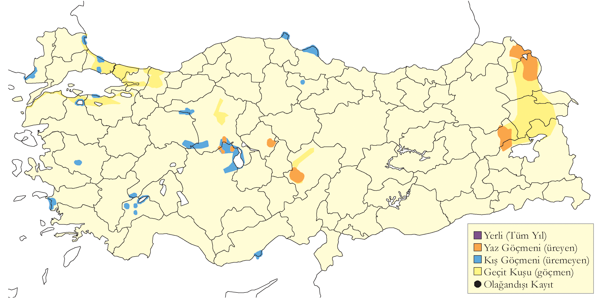
\includegraphics{images/harita_Page_002.png}

\textbf{Üreme}

\textbf{Yuvalama Alanı:} Göllerdeki adalarda genellikle küçük gruplar
halinde ürer.\\
\textbf{Yuvası:} Kulu Gölü'nde gözlenen yuvası kuru toprağa kazılmış sığ
bir çukurdur ve çevredeki bitki örtüsü ile küçük tüylerle
astarlanmıştır. Ereğli Sazlığı'ndaki yuvası ise saz ve diğer sucul
bitkilerden oluşan, su seviyesinin üstünde kalan bir yapının üzerine
kurulmuştur.\\
\textbf{Yumurta Sayısı:} Türkiye'de yumurta sayısına ilişkin güvenilir
gözlem yoktur. Yuvadan ayrılmış beş yavru, en az beş yumurta koyduğunu
gösterir. Diğer ülkelerde genellikle 4-6 yumurta bırakır.\\
\textbf{Üreme Dönemi:} Mart sonunda yumurta koyar. En erken yavrular 23
Nisan 1988'de Kulu Gölü'nde, 27 Nisan 1988'de Sultansazlığı'nda, 30
Nisan 1968'de Mogan Gölü'nde ve 30 Nisan 1973'te Ereğli Sazlıkları'nda
gözlenmiştir. 20 Nisan 1996'da Marmara'da, 14 Mayıs 1969'da
Karadeniz'de, 16 Mayıs 1970'te ve 24 Haziran 1983'te Doğu Anadolu'da
kaydedilen yavrular gecikmiş üremeyi göstermektedir.

\textbf{Alttürler ve Sınıflandırma}

Ülkemizde \emph{rubrirostris} alttürü bulunur. Bu alttür turuncu
gagasıyla Batı ve Orta Avrupa'da bulunan pembe gagalı \emph{anser}
alttüründen ayrılır.

\section{Sakarca}\label{sakarca}

\emph{Anser albifrons}, Greater White-fronted Goose

\textbf{\emph{Lokal olarak bulunan ve zaman zaman kalabalık sürüler
oluşturan bir kış konuğudur.}}

Ekim sonu ile nisan başı arasında lokal olarak görülen bir kış
konuğudur. Genellikle ocak ve şubat aylarında daha yaygın ve yüksek
sayıda olur. Soğuk geçen kışlarda Türkiye'de kışlayan birey sayısı
artar. En kalabalık sürüler Meriç Nehri boyunca, Tuz Gölü çevresinde ve
Konya Ovası'nda yoğunlaşır. Büyük Menderes Deltası ve Doğu Akdeniz'deki
sulakalanlarda da önemli sayılarda toplanabilir. Son zamanlarda
Güneydoğu Anadolu'daki baraj göllerinde küçük sürüler halinde görülmeye
başlanmıştır. Nadiren yaz aylarında sulakalanlarda az sayıda birey
kalabilir.

Kış ortası su kuşu sayımlarında (KOSKS) ülke genelinde en yüksek sayı
1968-69 kışında 98.600 birey olarak kaydedilmiştir. 1987'de ise toplam
84.000 birey sayılmıştır. Ancak daha sonra kışlayan birey sayısında
ciddi bir düşüş yaşanmıştır. 1990'lı yıllarda genellikle 20.000-30.000
arasında değişen sayılar kaydedilmiş 1993'te 11.822 (DHKD 1993), 1999'da
3956 (DHKD 1999) ve 2005'te 3891 birey (Çağlayan et al. 2005) tespit
edilmiştir. Kışın soğuk geçtiği 11 Şubat 2006'da Büyükçekmece'de 15.000
birey sayılmıştır, bu da son yıllardaki en yüksek sayıdır. Dolayısıyla
Türkiye'de kışlayan nüfusun 1970'lerde 100.000'ler seviyesinden
2010'larda 5000 civarına indiği söylenebilir.

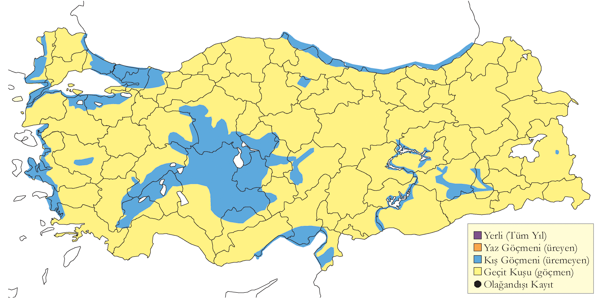
\includegraphics{images/harita_Page_003.png}

\textbf{Üreme}

Türkiye'de yuvalamaz. Avrasya ve Kuzey Amerika'nın tundra bölgelerinde
yuvalar.

\textbf{Alttürler ve Sınıflandırma}

Türkiye'de nominat alttürü bulunur.

\section{Küçük Sakarca}\label{kuxfcuxe7uxfck-sakarca}

\emph{Anser erythropus}, Lesser White-fronted Goose

\textbf{\emph{Az sayıda gelen düzenli kış konuğudur.}}

Her yıl çok az sayıda kaydedilen bir kış konuğudur. Sayıları genellikle
10'dan azdır ve diğer kaz türleriyle karışık olarak görülebilir. Bugüne
kadar Türkiye'ye gelen bireylerin İskandinavya'da üreyen ve Balkan
ülkelerinde kışlayan göç yoluna ait olduğu düşünülmüştür. Yunanistan'da
bir alanda kışlayan ve koruma çalışmaları sayesinde sayıları artan bir
sürünün kış ortasında oradan kaybolması, Marmara ve Ege bölgelerinde bir
kışlama alanı olabileceği ihtimalini doğurmuştur. Ancak yapılan
aramalara rağmen burada düzenli kullanılan bir kışlama alanı
bulunamamıştır.

Doğu Anadolu'da 20 Kasım 2004'te Haçlı Gölü'nde uydudan izlenen bir
birey sinyal verince, doğuda bir kışlama alanı olasılığı gündeme
gelmiştir (Morozov \& Aarvak 2004). Nitekim Van Gölü ve Erçek Gölü
kıyılarında sayıları 340'a ulaşan sürüler düzenli olarak tespit
edilmiştir. Bugün, Türkiye'de kışlayan ana nüfusun Doğu Anadolu'da
bulunduğu söylenebilir ((AOU) 2000).

2000 öncesindeki kayıtlara bakıldığında; 29 Aralık 1997'de Göksu
Deltası'nda bir birey (Kirwan et al. 2003), 23 Ocak 1993'te Göksu
Deltası'nda bir birey (DHKD 1993), 6 Nisan 1990'da Seyfe Gölü'nde 12
birey (Kirwan \& Martins 1994), 24 Aralık 1986'da Bafa Gölü'nde bir
erişkin ve iki genç birey (Kasparek 1988a) ve 16 Şubat 1967'de Kocabaş
Çayı'nın ağzında (Çanakkale) iki birey (OST 1969) kaydedilmiştir. 1945
ile 1965 yılları arasında ve ekim ile ocak aylarında, çoğunluğu
Büyükçekmece ve Küçükçekmece Göllerinden gelen 12 kayıt vardır. Ancak bu
kayıtlar, tür tanımını destekleyecek belgeden yoksundur (Kumerloeve
1970a).

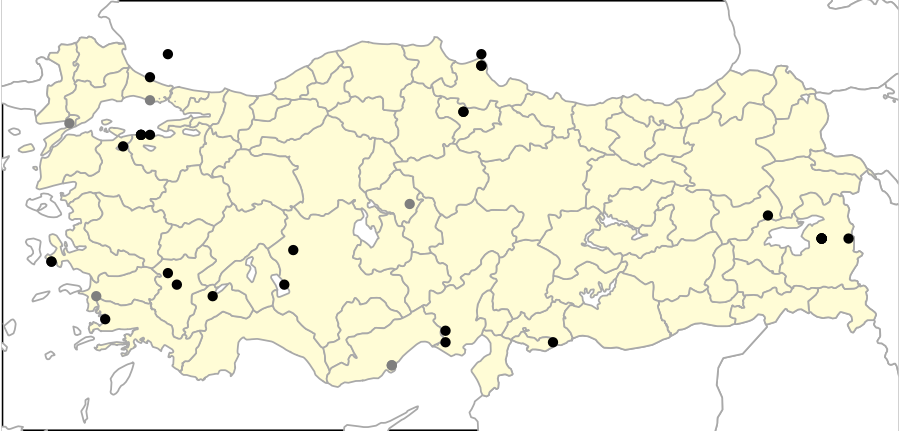
\includegraphics[width=6.25in,height=\textheight]{images/harita_Anser_erythropus.png}

\textbf{Üreme}

Türkiye'de yuvalamaz. Kuzey İskandinavya'dan Doğu Sibirya'ya kadar
uzanan tundra kuşağında ürer.

\textbf{Alttürler ve Sınıflandırma}

Monotipik bir türdür.

\section{Tundra Kazı}\label{tundra-kazux131}

\emph{Anser serrirostris}, Tundra Bean Goose

\textbf{\emph{Nadiren gelen kış konuğudur.}}

2000 yılından sonra 5 kez kaydedilmiştir. 26 Şubat 2013'te Yedikır
Barajı'nda, 4-21 Şubat 2015'te Kızılırmak Deltası'nda birer birey
görülmüştür. 31 Ocak 2016'da Manyas Kuş Gölü'nde 3 birey kaydedilmiş,
aynı alanda 2-24 Ocak 2019'da yine 3 birey gözlenmiştir. Acıgöl'de 24
Aralık 2023 ile 3 Şubat 2024 arasında bir birey gözlenmiştir.

\emph{Tundra Kazı}, önceleri \emph{Tayga Kazı} ile beraber tek bir tür
altında \emph{Tarla Kazı} olarak sınıflandırılıyordu. Dolayısıyla,
taksonomik revizyonun yapıldığı tarihten önceki kayıtlarda \emph{Tarla
Kazı} olarak tanımlanmıştır. 2000 yılından sonra çekilen fotoğraflarda
özellikle gaga renklenmesi incelenmiş ve bu kuşların tamamı \emph{Tundra
Kazı} olarak tanımlanmıştır. Fotoğrafı veya betimlemesi olmayan eski
kayıtların hangi türe ait olduğu ise belirsiz kalacaktır.

\emph{Tarla Kazı} olarak tanımlanmış kuşlar, Ege, Akdeniz ve İç
Anadolu'daki sulakalanlarda ara sıra yüksek sayılarda kaydedilmiştir.
1870'ler ve 1880'lerde Mersin'de toplanan bireyler (Schrader 1891) ilk
kayıtlar arasındadır. 1966-2000 yılları arasında çoğunlukla ocak ile
mart ayları arasında 15 kez kaydedilmiştir. 2 Mart 1965'te Ereğli ve
Karapınar arasında 90 birey (Kumerloeve 1970a), 15-16 Ekim 1969'da
Karamık Sazlıkları'nda 13 birey (OST 1972), 30 Nisan 1988'de Seyfe
Gölü'nde, 30 Ocak 1992'de Marmara Gölü'nde 61 birey, 9 Ocak 1993'te
Büyükçekmece Gölü'nde 64 birey (DHKD 1993) ve 24 Ocak 1993'te Göksu
Deltası'nda bir birey (DHKD 1993) kaydedilmiştir. Türkiye'deki kışlayan
Sakarca sayılarındaki sert düşüş, muhtemelen \emph{Tarla Kazı} olarak
tanımlanmış kuşlar için de geçerlidir.

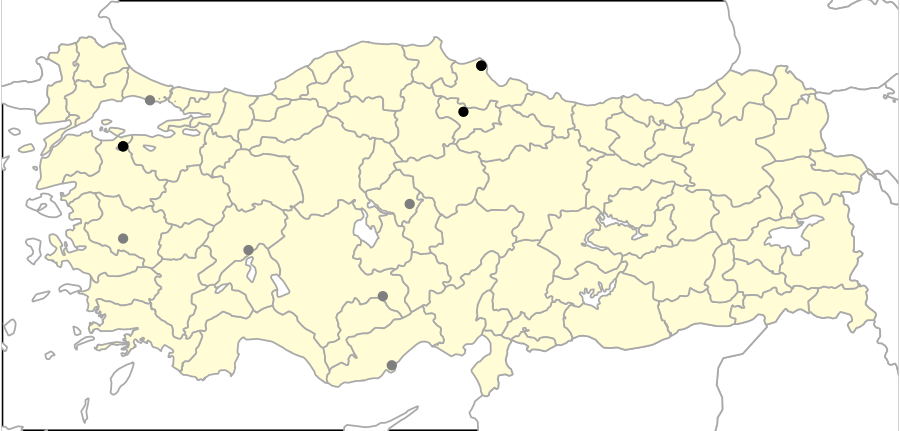
\includegraphics[width=6.25in,height=\textheight]{images/harita_Anser_serrirostris.png}

\textbf{Üreme}

Türkiye'de yuvalamaz. Üreme alanı Kuzey İskandinavya'dan Doğu Sibirya'ya
uzanan tundra kuşağındadır.

\textbf{Alttürler ve Sınıflandırma}

Tayga Kazı, yakın zamana kadar Tarla Kazı olarak bilinen bir türden
ayrılan yeni bir türdür. Beş alttüre sahip olan Tarla Kazı (\emph{Anser
fabalis}), iki gruba ayrılmıştır: \emph{fabalis}, \emph{johanseni} ve
\emph{middendorffii} alttürleri Tayga Kazı (\emph{Anser fabalis}),
\emph{serrirostris} ve \emph{rossicus} alttürleri ise Tundra Kazı
(\emph{Anser serrirostris}) olarak sınıflandırılmıştır.

\section{Yosun Kazı}\label{yosun-kazux131}

\emph{Branta bernicla}, Brant Goose

\textbf{\emph{Rastlantısal konuktur.}}

Batı Avrupa'nın Atlantik kıyılarında kışlayan bir türdür. Türkiye ile
yakın coğrafyasında rastlantısal bir konuktur. 6 Nisan 1981'de Küçük
Menderes Deltası'nda iki birey gözlenmiştir (Beaman 1986). 3-4 Eylül
1973'te Ardeşen açıklarında koyu karınlı \emph{bernicla} alttürüne ait
iki birey kaydedilmiştir (OST 1975). 1969 yılında Acıgöl'den gelen bir
iddia ise kabul edilmemiştir (Dijksen \& Kasparek 1988). 7 Şubat 1945'te
Büyükçekmece'de bir birey Prenses Zeyneb Halim tarafından vurulmuştur,
ancak kuşun gövdesi korunamamıştır (Kumerloeve 1970a). Ocak 1889'da
kışın soğuk geçtiği bir yılda İstanbul Maltepe'de düzenli olarak, Şubat
1891'de ise büyük sürüler halinde İstanbul Kadıköy'de görülmüştür
(Mathey-Dupraz 1920--24).

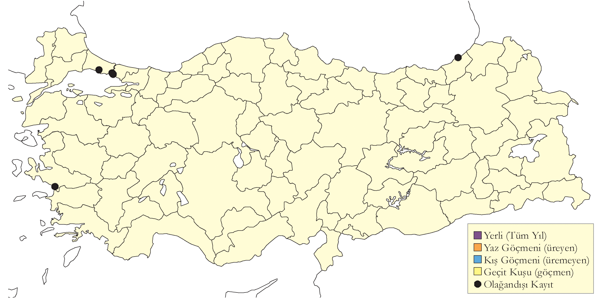
\includegraphics{images/harita_Page_005.png}

\textbf{Üreme}

Türkiye'de yuvalamaz. Orta ve Kuzey Sibirya'nın Kutup Denizi kıyılarında
yuvalar.

\textbf{Alttürler ve Sınıflandırma}

Bir kayıtta kuşun alttürü \emph{bernicla} olarak tanımlanmıştır. Keza,
Kuzeybatı Avrupa'da kışlayan \emph{bernicla} alttürünün Türkiye'de
görülmesi olasıdır. Yunanistan'daki bir kayıt da bu alttüre aittir
(Handrinos \& Akriotis 1997).

\section{Ak Yanaklı Kaz}\label{ak-yanaklux131-kaz}

\emph{Branta leucopsis}, Barnacle Goose

\textbf{\emph{Rastlantısal konuktur.}}

5 Ocak 2003'te Büyükçekmece Gölü'nde bir birey gözlenmiş ve detaylı
olarak belgelenmiştir. 1946/47 kışında Sakarya Deltası'nda bir birey,
1961 sonbahar/kışında ise başka bir birey vurulmuştur. İkinci kuşun
tahniti Eylül 1964'te Ankara'da bulunmuş, ancak sahibi tahniti satmaya
yanaşmamıştır (Kumerloeve 1966). Bu iki kaydın belgeleri yetersizdir
(Kumerloeve 1970a).

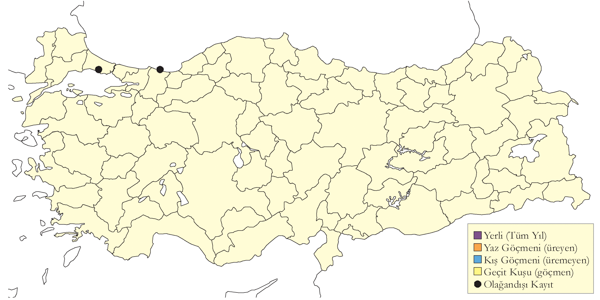
\includegraphics{images/harita_Page_006.png}

\textbf{Üreme}

Türkiye'de yuvalamaz. Grönland, İzlanda, Kuzey Batı Rusya ve Baltık
Denizi kıyılarında yuvalar.

\textbf{Alttürler ve Sınıflandırma}

Monotipik bir türdür.

\section{Sibirya Kazı}\label{sibirya-kazux131}

\emph{Branta ruficollis}, Red-breasted Goose

\textbf{\emph{Az sayıda gelen düzensiz kış konuğudur.}}

Türkiye'de düzenli kışladığı bilinen bir alan yoktur; ana kışlama alanı
Romanya ve Bulgaristan'ın Karadeniz kıyısıdır. Özellikle soğuk kışlarda,
bireyler veya gruplar halinde Türkiye'ye inerler. 1964 ile 2008 yılları
arasında 64 kayda rastlanmıştır. Bu kayıtların 15'i Marmara'da, 12'si İç
Anadolu'da, 8'i Karadeniz'de, 6'sı Akdeniz'de ve 4'ü Ege'de alınmıştır.
Kayıtların çoğu aralık sonu ile şubat başı arasındadır. Çoğunlukla bir
veya birkaç kuş sayılmış, ancak 5 kayıtta 40 ila 100 bireyden oluşan
nispeten kalabalık sürüler de gözlenmiştir. 2001/2002 kışında Türkiye
genelinde 192 birey sayılmıştır.

Ülke genelinde yaygın olarak av mağazaları ve avcılık kulüplerinde
tahnit örneklerine rastlanması ve avcıların gözlem beyanları (Dijksen \&
Kasparek 1985), bu kuşların kayıtlardan daha yaygın olabileceğini
gösterir. İç Anadolu'dan gelen eski kayıtlar, Kış Ortası Su Kuş
Sayımları sırasında kalabalık kaz sürülerinin sistematik incelenmesi ile
ortaya çıkmıştır. Sakarca kazı sürüleri içinde bu türün fark edilmemesi
olasıdır.

1946/47 kışında Küçükçekmece'de Kosswig tarafından gözlenmiştir
(Kumerloeve 1966). 1947 veya 1954 yıllarında kış boyunca (27 Kasım - 6
Mart) Büyükçekmece ve Meriç Nehri civarında düzenli olarak 9 birey ve
Beylik Mandra'da 2 birey kaydedilmiştir (Kumerloeve 1970a). 1959 yılında
belirtilmemiş bir alanda İshakoğlu tarafından sekiz birey gözlenmiş ve
bir birey vurulmuştur (Makatsch 1950). 12 Kasım 1964'te Kuyucuk Gölü'nde
400 boz kazın arasında 2 erişkin ve 1 genç birey kaydedilmiştir
(Kumerloeve 1964). 17 Ocak 1965 tarihinde Çekmece'de E. Hirzel
tarafından 3 birey görülmüştür.

Türkiye'de açıklama gerektiren bir yaz veya üreme kaydı vardır. 5
Ağustos 1982'de Erçek Gölü'nde 14 erişkin ve 8 yavru kaydedilmiştir
(Kasparek \& Ven 1983). Bu kayıt ya hatalı bir gözlem olarak kabul
edilmeli ya da avcılar tarafından yakalanıp evcilleştirilen kuşların
üremesinin bir sonucu olarak yorumlanmalıdır.

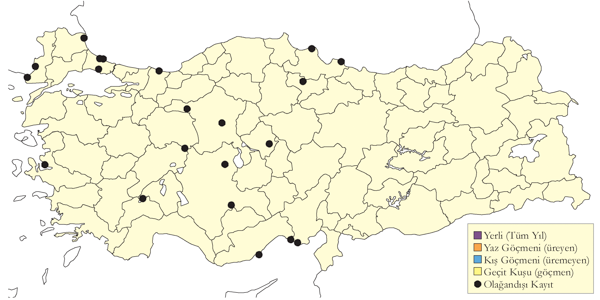
\includegraphics{images/harita_Page_007.png}

\textbf{Üreme}

Türkiye'de yuvalamaz. Doğu Sibirya'da tundra kuşağında yuvalar.

\textbf{Alttürler ve Sınıflandırma}

Monotipik bir türdür.

\section{Sessiz Kuğu}\label{sessiz-kuux11fu}

\emph{Cygnus olor}, Mute Swan

\textbf{\emph{Lokal olarak az sayıda yuvalar. Yaygın olarak ve nispeten
çok sayıda bulunan bir kış konuğudur.}}

Üreme kayıtlarının çoğu üç alandan gelir: Gala Gölü, Gediz Deltası ve
Kızılırmak Deltası. Ulusal üreme popülasyonu muhtemelen 20 çiftten daha
azdır. Kızılırmak Deltası'ndan alınan ilk muhtemel üreme kaydı 1968
yılına aittir (Dijksen \& Kasparek 1985).

Geçmişte, birkaç alanda yüzlerce çiftlik bir üreme nüfusu bulunuyordu.
Marmara Gölü'nde 50 çift, Akşehir Gölü'nde ise 100 çift üremiştir
(Kumerloeve 1961). Ereğli Sazlığı en çok gözlem kaydının alındığı
alandır. Lenz burada 1968'de 11 yuva, 1969'da bir yuva ve 1970'de üç
yuva bulmuştur. Ereğli Sazlığı'nın yok olması ayrıntılı olarak
belgelenmiştir (Kılıç \& Kasparek 1990), bu nedenle üreyen nüfusun
azalışı da gözlenmiştir. Eski üreme alanlarında yok olmasının başlıca
nedeni sulakalanların kurutulmasıdır.

Kış aylarında Karadeniz, Marmara ve Ege Bölgelerinde yaygın olarak en
yüksek sayılarda gözlenir. Toplam kışlama popülasyonu 1000-10000 birey
arasında değişmektedir. Meriç Deltası ve Gala Gölü kışlayan nüfusun
büyük kısmının toplandığı alanlardır. 1993'te 1244, 1999'da 8900 ve
2003'te 2000 birey kaydedilmiştir (DHKD 1993, 1999). Kışın sert geçtiği
yıllarda bu sayı artmakta olup, 1999'da ülke genelinde toplamda 9088
birey kaydedilmiştir.

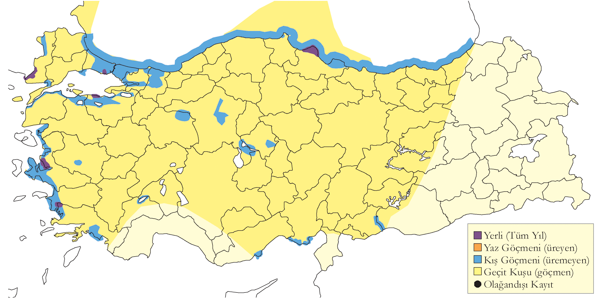
\includegraphics{images/harita_Page_008.png}

\textbf{Üreme}

\textbf{Yuvalama Alanı:} Geniş sazlık alanlar, su aynası bulunan büyük
göller ve bataklıklarda yuvalar.\\
\textbf{Yuvası:} Türkiye'de henüz bir yuva tarifi yapılmamıştır. Diğer
bölgelerde yuva su kıyısındaki zemin üzerinde, küçük bir adacıkta ya da
sığ sudaki sazların üstüne kurulur. Yuva, saz ve diğer sucul bitkilerden
oluşan büyük bir yığının ortasında çukur şekilli bir yapıdır.\\
\textbf{Yumurta Sayısı:} Türkiye'deki yumurta sayısı bilinmez. Ancak
Türkiye dışındaki yuvalarda genellikle 5-7 yumurta bıraktığı
bilinmektedir.\\
\textbf{Üreme Dönemi:} Nisan başında yumurtlamaya başlar, yavrular ise
mayıs ve temmuz ayları arasında görülür. \textbf{EGE.} 13 Mayıs 1899'da
İzmir'de bir sazlıkta yuvalayan bir çift kaydedilmiştir (Selous 1900).
\textbf{İÇA.} 6 Temmuz 1976'da Ereğli Sazlığı'nda bir çift ve 4-5 genç
yavru, 17 Temmuz 1982'de bir çift ve dört genç, 16 Mayıs 1987'de ise
yumurtadan yeni çıkmış yavrular gözlenmiştir.

\textbf{Alttürler ve Sınıflandırma}

Monotipik bir türdür.

\section{Küçük Kuğu}\label{kuxfcuxe7uxfck-kuux11fu}

\emph{Cygnus columbianus}, Tundra Swan

\textbf{\emph{Lokal olarak ve az sayıda bulunan bir kış konuğudur.}}

1993 yılına kadar nadir bir kış konuğu olduğu düşünülmüştür. Ancak daha
sonra, önce Burdur Gölü ve Göller Bölgesi'nde, ardından Meriç
Deltası'nda düzenli olarak bulunduğu tespit edilmiştir. Meriç
Deltası'nda, karışık ve kalabalık kuğu sürüleri içinde sayıları 1000'e
kadar ulaşabilir. İç Anadolu ve Göller Bölgesi'nde ise küçük gruplar
halinde bulunur. Genellikle kasım ve nisan ayları arasında gözlenir.

Türkiye'de kışlayan kuşların üreme alanları ve göç koridorları tespit
edilmiştir (Vangeluwe et al. 2018). 2015-2017 yıllarında GPS ve GMS
vericileriyle yapılan çalışmada, yuvalama alanlarının Yamalo-Nenets
Özerk Bölgesi'ndeki Yamal olduğu belirlenmiştir. Göç sırasında Ob Koyu,
Turgay Ovaları, Kuzey Hazar Kıyıları ve Azov Denizi gibi durak alanları
üzerinden göç ettikleri ortaya çıkmıştır.

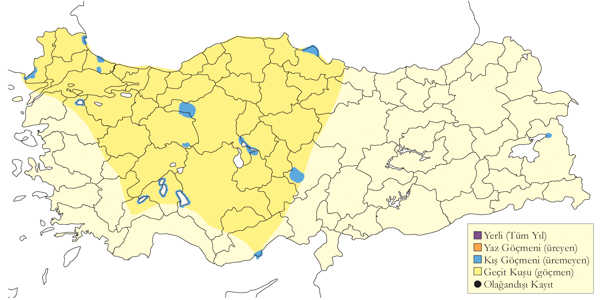
\includegraphics{images/harita_Page_009.png}

\textbf{Üreme}

Türkiye'de yuvalamaz. Sibirya Tundra kuşağında yuvalar.

\textbf{Alttürler ve Sınıflandırma}

Türkiye'de Eski Dünya'da yaşayan \emph{bewickii} alttürü bulunur; bu
alttür, gaga kökü ve yüz derisinin sarı olmasıyla tanınır. Amerika'da
yaşayan \emph{columbianus} alttürü ise siyah gaga ve siyah yüz derisi
ile kolaylıkla ayırt edilebilir.

\section{Ötücü Kuğu}\label{uxf6tuxfccuxfc-kuux11fu}

\emph{Cygnus cygnus}, Whooper Swan

\textbf{\emph{Yaygın olarak ve az sayıda görülen bir kış konuğudur.}}

Ekim sonu ile nisan başı arasında yaygın olarak az sayıda görülen bir
kış konuğudur. Ocak ve şubat aylarında en yüksek sayıya ulaşır.
Trakya'da Meriç Deltası hem Türkiye'deki ana toplama bölgesidir, üstelik
türün Balkanlar'daki en önemli kışlama alanıdır. 25 Ocak 1998'de Meriç
Deltası'nda 1200 birey kaydedilmiş, bu Türkiye'deki en yüksek sayıdır
(Boyla \& Eken 1998). Türkiye'ye gelen kuşlar, Ukrayna ve Kırım ile Batı
Karadeniz Bölgesi arasındaki deniz üzeri göç rotasını kullanır (Brazil
2003). Doğuda, 30 Ekim 1995'te Sodalı Gölü'nde 164 birey (Adızel 1998),
1992'de Diyarbakır Kabaklı Barajı'nda 133 birey kaydedilmiştir (DHKD
1992).

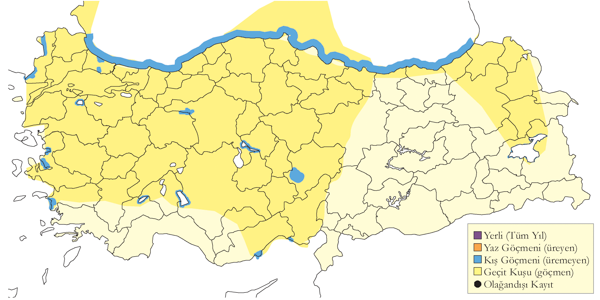
\includegraphics{images/harita_Page_010.png}

\textbf{Üreme}

Türkiye'de yuvalamaz. Üreme bölgesi Kuzey Avrasya'dadır

\textbf{Alttürler ve Sınıflandırma}

Monotipik bir türdür.

\section{Nil Kazı}\label{nil-kazux131}

\emph{Alopochen aegyptiaca}, Egyptian Goose

\textbf{\emph{Durumu belirsizdir. Çoğunlukla egzotik tür kategorisinde
değerlendirilir.}}

28 Nisan 1986'da Kulu Gölü'nde gözlenen bireyin doğal ve rastlantısal
bir konuk olduğu düşünülmüştür. 11 Nisan 1911'de Urfa'nın güneyinde iki
birey gördüğünü söyleyen Weigold'un (1912-13) kaydı kabul edilmemiştir
(Kasparek 1992).

İstanbul ve Ankara'da gözlenen kuşların esaretten kaçmış olabileceği
düşünülmektedir. 6-13 Temmuz 2002'de Ankara'daki bir parkta bir çift
fotoğraflanmış; 31 Mart 2012'de İstanbul Riva'da, 13 Mart 2012'de Ankara
Hacettepe Kampüsü'nde, 5-24 Kasım 2013'de Etimesgut'ta ve 25 Mayıs-13
Haziran 2014'de Eymir Gölü'nde birer birey gözlenmiştir.

1906 ve 1928 yılları arasında Kıbrıs'ta nadir görülen bir kış göçmeni
olarak kaydedilmiş ve 1958, 1962 ve 1989 yıllarında bireyler
gözlenmiştir. Eskiden Suriye ve Filistin'de ürediği düşünülmüş (Vaurie
1965), ancak sonrasında Suriye'de hiçbir güvenilir kaydın olmadığına
karar verilmiştir (Kumerloeve 1967a, Baumgart et al. 1995).

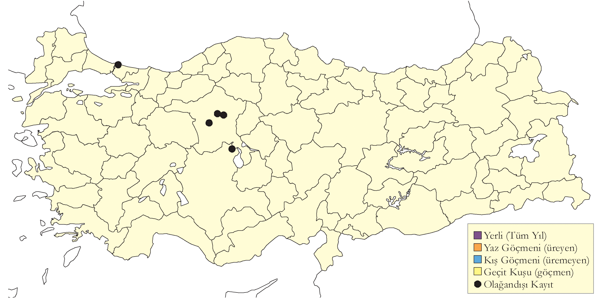
\includegraphics{images/harita_Page_011.png}

\textbf{Üreme}

Türkiye'de yuvalamaz. Üreme alanları çoğunlukla Sahra Altı Afrika'dadır.

\textbf{Alttürler ve Sınıflandırma}

Monotipik bir türdür.

\section{Suna}\label{suna}

\emph{Tadorna tadorna}, Common Shelduck

\textbf{\emph{Lokal olarak az sayıda ürer. Aynı zamanda lokal olarak çok
sayıda bulunabilen bir kış konuğudur.}}

Ege Bölgesi, Göller Bölgesi, İç ve Doğu Anadolu'da geniş ve tuzlu
sulakalanlarda ürer. Başlıca üreme alanları Gediz Deltası, Bolluk Gölü,
Kulu Gölü, Tuz Gölü ve Van Gölü çevresidir. Gediz Deltası'nda 1996
yılında üreyen popülasyonun 8 çift olduğu tahmin edilmiştir (Eken
1997a). 24 Haziran 1992'de Bolluk Gölü'ndeki bir adada 12 yuva tespit
edilmiştir.

Üreme sonrası tüy değiştiren kuşlar, ağustos ile ekim ayları arasında
toplanır. Bu dönemde Erçek Gölü'nde 2500 birey, Kulu Gölü'nde ise 700
birey sayılmıştır.

Kışlayan toplam nüfus genellikle 1000-5000 birey arasında değişir. Ana
kışlama alanı olan Yumurtalık Lagünü'nde, 16 Şubat 2006'da 5390 birey
kaydedilmiştir. Acıgöl'de ise 1969-70 yıllarında 3450 birey, 1968-69
yıllarında 4900 birey, 2004 yılında 1802 birey ve 2005 yılında 2928
birey sayılmıştır. Diğer alanlarda daha küçük gruplar halinde kışlar.

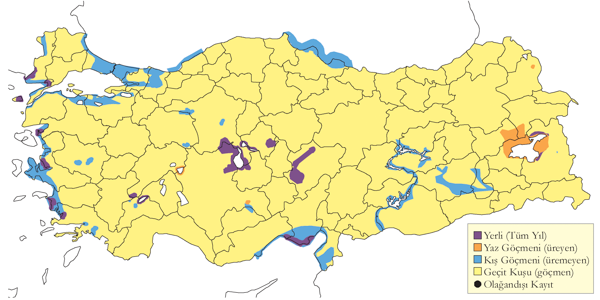
\includegraphics{images/harita_Page_012.png}

\textbf{Üreme}

\textbf{Yuvalama Alanı:} Geniş, sığ ve tuzlu sulakalanlarda, adalar,
sedde duvarları ve çalı altlarında yuvalar.\\
\textbf{Yuvası:} Avrupa'da yuvaların çoğu tavşan oyuklarında, tünelin
1-2 metre içinde bulunur. Ancak Türkiye'deki yuvalar genellikle
yerdedir. Bolluk Gölü'ndeki yuvaların bazıları tamamen açıkta, bazıları
ise kısmen ya da tamamen çalı altında, bir tanesi ise doğal bir oyuğun
içinde bulunmuştur.\\
\textbf{Yumurta Sayısı:} Genellikle 6-9 yumurta bıraktığı gözlenmiştir.
Bolluk Gölü'ndeki yuvalarda gözlenen 10-18 yumurtanın, birden fazla dişi
tarafından bırakılmış olması muhtemeldir.\\
\textbf{Üreme Dönemi:} Gediz Deltası'nda haziran başında yavrular
gözlenmiştir (Eken 1997a). İç Anadolu'da nisan sonu ile haziran başında,
Doğu Anadolu'da ise haziran ortasında yumurtladığı düşünülmektedir.

\textbf{Alttürler ve Sınıflandırma}

Monotipik bir türdür.

\section{Angıt}\label{angux131t}

\emph{Tadorna ferruginea}, Ruddy Shelduck

\textbf{\emph{Yaygın ve çok sayıda bulunan yerli türdür. Kışın göç alır,
sayıları artar.}}

Üremek için genellikle yüksek kesimlerdeki küçük gölcükler, baraj
gölleri, ıslak çayırlar ve dereleri tercih eder; birçok ördek ve kaz
türünün aksine büyük sulakalanlarda yuvalamaz. İlk tahminlere göre
üreyen popülasyonun 4000 ile 8000 çift arasında olduğu öne sürülmüştür
(Tucker \& Heath 1994). Ancak, kış ortası su kuşu sayımlarına dayanarak
popülasyonun azaldığı düşünülmüş ve üreyen popülasyonun 1200-5100 çift
olduğu tahmin edilmiştir (Emirogullari et al.).

Temmuz ve eylül ayları arasında tüy değişimi için bazı sulakalanlarda
büyük sürüler halinde toplanır. Erçek Gölü'nde 20.000, Sultan
Sazlığı'nda 11.000, Kulu Gölü'nde 10.000 ve Eylül 1936'da, bugün
kurutulmuş olan Emir Gölü'nde 10.000-15.000 birey sayılmıştır. Kış
öncesinde Kasım 2004'te Sarıyar Barajı'nda 8.000 birey ve Kuyucuk
Gölü'nde 6.000 birey kaydedilmiştir.

Kış aylarında daha yaygın olarak görülür. En yüksek kış sayımında
Türkiye genelinde 10.115 birey kaydedilmiş olup (Çağlayan et al. 2005),
genellikle 4000-4500 birey sayılmıştır. Ocak-Şubat 1993'te sadece 711
birey, 18 Ocak 2004'te Sarıyar Barajı'nda 5636 birey ve 18 Şubat 2006'da
7641 birey kaydedilmiştir. İç Anadolu'da üreme sonrası toplanan
sürülerde bir azalma gözlenirken, baraj göllerinin sayısında artış
olmuştur. Kış sayımı toplamlarının yaz sonu toplamlarından düşük olması,
türün dağınık şekilde kışladığını veya kış aylarında güneye göç ettiğini
göstermektedir. Toplam kışlayan nüfusun 2600 ile 28.500 birey arasında
değiştiği tahmin edilmektedir (Emirogullari et al.).

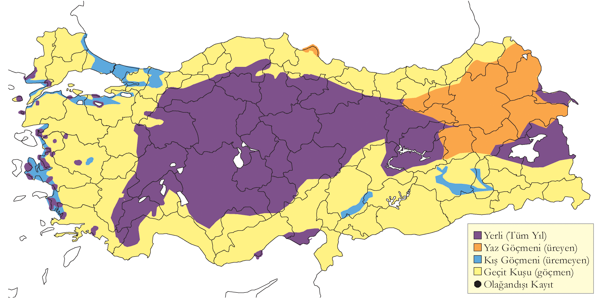
\includegraphics{images/harita_Page_013.png}

\textbf{Üreme}

\textbf{Yuvalama Alanı:} Genellikle göl kenarındaki sarp kayalıklarda,
tepelerde ve yamaçlardaki çukur ve çatlaklarda, açık alanlarda yuvalar.
Sıkça kayalıklarda yuva yaptığı gözlenmiştir. Beyşehir Gölü'ndeki bir
adada, kayaların ve harabelerin taşları arasında ürediği kaydedilmiştir.
22-24 Mayıs 1998'de Ereğli yakınlarındaki bir kayalıkta, muhtemelen eski
bir Kızıl Şahin yuvasında kuluçkaya yattığı gözlenmiştir.\\
\textbf{Yuvası:} Türkiye'de yuvası bitki artıkları, hav tüyleri ve bazı
diğer tüylerle kaplanmış bir oyuk şeklindedir. 30 Nisan 2003'te Akköy
yakınlarındaki dik bir yamaca giren bir dişi, muhtemelen bir tavşan
yuvası olan bir oyuğa girerken gözlenmiş, ancak oyuğun derin olması
nedeniyle yuva incelenememiştir.\\
\textbf{Yumurta Sayısı:} Genellikle 8-12 yumurta bıraktığı
kaydedilmiştir.\\
\textbf{Üreme Dönemi:} Akdeniz ve Ege bölgelerinde mart sonu yumurtlama
başlar. Diğer bölgelerde kuluçka nisan ve mayıs aylarında gerçekleşir.

\textbf{Alttürler ve Sınıflandırma}

Monotipik bir türdür.

\section{Boz Ördek}\label{boz-uxf6rdek}

\emph{Mareca strepera}, Gadwall

\textbf{Lokal olarak birkaç alanda yuvalar. Yaygın olarak nispeten az
sayılarda görülen bir kış konuğudur.}

Kızılırmak Deltası, bu türün Türkiye'deki en önemli üreme alanıdır ve
yaklaşık 200 çift burada ürer. Türkiye'de toplam üreyen popülasyonun 500
ile 5000 çift arasında olduğu düşünülmüştür (Tucker \& Heath 1994).
Ancak, günümüzde bu sayının azaldığı açıktır.

İç Anadolu'daki ilkbahar göçü marttan nisan başına kadar belirgin bir
şekilde gözlenir. Akdeniz'deki kıyısal sulakalanlarda ise nadiren
1000'den fazla birey kaydedilir. Kış ortası sayımlarda 1967'de Manyas
Gölü'nde 5000, 1969'da Akşehir Gölü'nde 7500 ve 1971'de Hotamış
Sazlığı'nda 2490 birey sayılmıştır. 1967-1973 yılları arasında ülke
genelinde çoğunlukla 3000'den fazla birey kaydedilirken, 1986-2005
yılları arasında bu sayı 1000-1500 seviyelerine düşmüştür. Son yıllarda
ise yeniden artış göstermiş ve 2020 kışında Kızılırmak Deltası'nda
10.000'den fazla birey sayılmıştır.

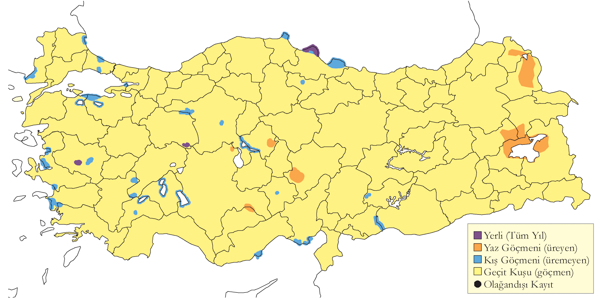
\includegraphics{images/harita_Page_014.png}

\textbf{Üreme}

\textbf{Yuvalama Alanı:} Göl kıyılarında ve adalarındaki yoğun bitki
örtüsü, sazlıklar ve sık bitkilerle kaplı taşkın alanlarda yuvalar.
Kızılırmak Deltası, Karamık Gölü, Kulu Gölü, Bolluk Gölü, Mogan Gölü,
Ahlat Sazlıkları, Haçlı Gölü ve Van Gölü'nde yuvaladığı gözlenmiştir.\\
\textbf{Yuvası:} Yuva, yerde bir çukura kurulur ve bitkisel malzeme ile
dişinin tüyleriyle kaplanır.\\
\textbf{Yumurta Sayısı:} Türkiye'deki yuvalarda yumurta sayısı 6-15
arasında değişir. İç Anadolu'da 7-15 yumurtalı yuvalar gözlenmiş ve bu
yuvaların bir kısmında 1 ila 6 yumurtanın başka ördek türlerine ait
olduğu tespit edilmiştir. Kulu Gölü'ndeki yuvalarda 6 Mayıs 1972'de 3-11
yumurta ve 14 Temmuz 1971'de 7 yumurta sayılmıştır (Kasparek 1987). 17
Mayıs 2004'te Bolluk Gölü'ndeki bir yuvada 8 yumurta bulunmuştur.\\
\textbf{Üreme Dönemi:} Kızılırmak Deltası'nda nisan başında yumurtlamaya
başlar (Hustings \& Dijk 1994). İç Anadolu'da nisan sonu ile temmuz
arasında, Doğu Anadolu'da ise haziran ile eylül arasında yavrulara
rastlanmıştır.

\textbf{Alttürler ve Sınıflandırma}

Türkiye'de nominat alttür görülür. Tür eskiden \emph{Anas} cinsi altında
sınıflandırılıyordu.

\section{Fiyu}\label{fiyu}

\emph{Mareca penelope}, Eurasian Wigeon

\textbf{\emph{Yaygın olarak çok sayıda bulunan kış konuğu ve geçit
türüdür.}}

Ege, Akdeniz ve İç Anadolu'nun sulakalanlarında kalabalık sürüler
halinde kışlar. 1960'lı ve 1970'li yıllarda düzenli olarak ortalama
150.000 birey sayılmıştır. En yüksek sayılar 1968'de 208.600, 1969'da
ise 458.800 birey olarak kaydedilmiştir. Ancak günümüze gelindiğinde
ciddi bir düşüş yaşanmış, 1986 ile 2005 yılları arasındaki düzenli
sayımlarda yalnızca dört yıl 40.000'den fazla birey kaydedilebilmiştir.
Genellikle eylül sonunda gelir ve nisan sonuna kadar kalır.

İç Anadolu'da mart sonu ve nisan başı arasında yüksek sayılarda göç
eder. Bazı göçmen bireyler mayıs sonuna kadar bölgede kalır. Nadiren de
olsa, İç ve Doğu Anadolu'da üremeden yazı geçiren bireyler gözlenebilir.

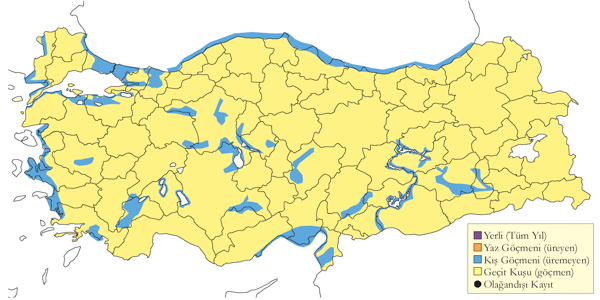
\includegraphics{images/harita_Page_015.png}

\textbf{Üreme}

Türkiye'de yuvalamaz. Kuzey Avrupa'da yuvalar.

\textbf{Alttürler ve Sınıflandırma}

Monotipik bir türdür. Eskiden \emph{Anas} cinsi altında
sınıflandırılırdı.

\section{Yeşilbaş}\label{yeux15filbaux15f}

\emph{Anas platyrhynchos}, Mallard

\textbf{\emph{Yaygın olarak üreyen yerli bir türdür. Kışın göç alır,
yüksek sayılara ulaşabilir.}}

Uygun yaşam alanlarının bulunduğu bölgelerde az sayıda yuvalar. En
yaygın olarak İç Anadolu Bölgesi'ndeki sulakalanlarda görülür, diğer
bölgelerde ise oldukça lokal bir dağılım gösterir. En yüksek yuvalama
sayısı, 400-600 çiftin kaydedildiği Kızılırmak Deltası'nda olmuştur
(Hustings \& Dijk 1994).

Sonbaharda göç alır ve popülasyonu artar. Kışlayan gruplar nisan başına
kadar bölgede kalır. En yüksek sayılarda Karadeniz, Marmara ve Ege
bölgelerinde kaydedilirken, Akdeniz ve İç Anadolu'da nispeten az sayıda,
Güneydoğu Anadolu ve Doğu Anadolu'da ise çok daha az sayıda bulunur.
2000 ve 2020 yılları arasında kışlayan nüfus ortalama 20.000 birey
civarındayken, kışın sert geçtiği 2005 yılında Türkiye genelinde toplam
106.140 birey ve Kızılırmak Deltası'nda 50.000 birey sayılmıştır.

1960'lı ve 1970'li yıllarda kışlayan popülasyonun 100.000'ler
seviyesinde olduğu bildirilmiştir. 1967 yılında Kızılırmak ve Yeşilırmak
Deltası'nda yaklaşık 52.000, Büyük Menderes Deltası'nda 42.000; 1968
yılında Manyas ve Uluabat Gölleri'nde 42.000; 1969 yılında Büyük
Menderes Deltası'nda 80.000, Akyatan Lagünü'nde 40.000 ve Amik Gölü'nde
30.000; 1970 yılında ise Meriç Deltası'nda 34.500 ve Sultansazlığı'nda
30.000 birey kaydedilmiştir.

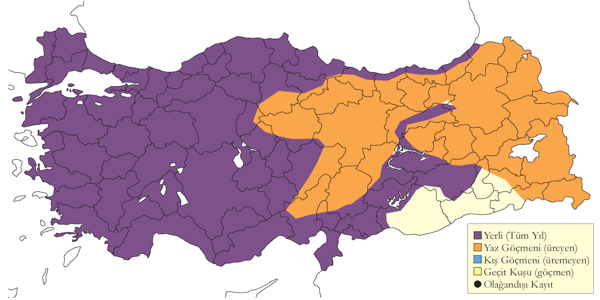
\includegraphics{images/harita_Page_016.png}

\textbf{Üreme}

\textbf{Yuvalama Alanı:} Göl ve nehir adalarında, sazlıklarda veya göl,
sazlık ve subasar çayırların kıyılarındaki sık bitki örtüsü içinde
yuvalar.\\
\textbf{Yuvası:} Yuvasını genellikle bitki örtüsünün altına, topraktaki
bir oyuğa yapar. Diğer bölgelerde ağaç kovuklarına veya karga gibi
kuşların ağaçlardaki eski yuvalarına yuvaladığı bilinir; ancak
Türkiye'de bu tür yuvalara henüz rastlanmamıştır.\\
\textbf{Yumurta Sayısı:} Genellikle 5-9 yumurta bırakır, ancak yumurta
sayısı 2-14 arasında değişebilir. Bir yuvadaki yumurtaların 14'ten fazla
olması, birden fazla dişinin aynı yuvaya yumurtladığını gösterir.\\
\textbf{Üreme Dönemi:} Kıyı bölgelerinde marttan itibaren, diğer
bölgelerde ise nisan veya mayısta yumurtlar. Yavrular mayıs başından
temmuz sonuna kadar görülebilir. \textbf{Marmara:} 18 Nisan 1993'te
Kocaçay Deltası'nda yavrularıyla gözlenen bir dişi, en erken üreme
kaydıdır (Ertan 1996). \textbf{Karadeniz:} 19-20 Mayıs 1992'de Yeniçağa
Gölü'nde yuvalarda hem yumurta hem yavrular gözlenmiştir. 5 Mayıs
1992'de Kızılırmak Deltası'nda sezonun ilk yavruları görülmüştür
(Hustings \& Dijk 1994). 16 Mayıs 1967'de Manyas Gölü'nde dokuz
yumurtalı bir yuva kaydedilmiştir. 20 Haziran 1973'te Trakya'da altı
yavrulu bir dişi gözlenmiştir. \textbf{İç Anadolu:} 1971'de Yarma'daki
birçok yuvada diğer türlerin yumurtalarına rastlanmıştır; örneğin, bir
yuvada 17 Yeşilbaş, üç Boz Ördek ve üç Macar Ördeği yumurtası
tanınmıştır. 13-15 Temmuz 1971'de Kulu Gölü'nde sekiz yuva incelenmiş ve
yuvalarda 2-12 yumurta bulunmuştur (Kasparek 1987). Başka bir tarihte,
mayıs ve haziran aylarında yumurtalı yuvalar ve mayıs ortasından
itibaren yavrular gözlenmiştir. \textbf{Doğu Anadolu:} En erken kayıt,
14 Haziran 1968'de Erçek Gölü'nde kaydedilen yavrulardır. Aynı yerde 28
Haziran 1968'de beş ve sekiz yumurtalı iki yuva bulunmuş, 9 Haziran
2001'de Balık Gölü'nde iki yumurtalı yuva kaydedilmiştir (Kasparek \&
Ven 1983).

\textbf{Alttürler ve Sınıflandırma}

Türkiye'de nominat alttürü bulunur.

\section{Kaşıkgaga}\label{kaux15fux131kgaga}

\emph{Spatula clypeata}, Northern Shoveler

\textbf{\emph{Lokal olarak az sayıda yuvalar. Aynı zamanda yaygın olarak
çok sayıda bulunan bir geçit türü ve kış konuğudur.}}

İç Anadolu ve Doğu Anadolu'daki birkaç büyük sulakalan ile Kızılırmak
Deltası'nda yuvalar (Boyla et al. 2018). 1970'lerde Kulu Gölü ve
Kızılırmak Deltası bilinen üreme alanlarıdır.

Tüm bölgelerde yaygın olarak kaydedilen bir geçit türüdür. Göçmen
gruplar, ilkbaharda mart başından nisan sonuna kadar, sonbaharda ise
eylül ortasından kasım başına kadar zaman zaman yüksek sayılarda
görülür. Eylül ayında Kulu Gölü'nde 7000, Sultansazlığı'nda 9000 ve mart
sonunda Kızılırmak Deltası'nda 4500 birey sayılmıştır.

Ülkenin batı ve orta bölgelerinde kışlar. 2000 ile 2020 yılları arasında
ülke çapında kışlayan kuş sayısı genellikle 5000 bireyin altında
kalmıştır; ancak kışın soğuk geçtiği 2005 yılında 13.576 birey
sayılmıştır. 1990'lı yıllarda daha yüksek sayılar kaydedilirdi; örneğin,
1993'te toplam 7898 birey, 1999'da ise 13.114 birey kaydedilmiştir. Daha
önceki yıllarda yapılan sayımlarda; 1967'de Büyük Menderes Deltası'nda
23.000, Kızılırmak Deltası'nda 8000 birey ve 1993'te 4564 birey
sayılmıştır. 1967-1973 yılları arasında İç Anadolu'daki alanlarda
3000'den fazla bireyden oluşan sürüler olağandı.

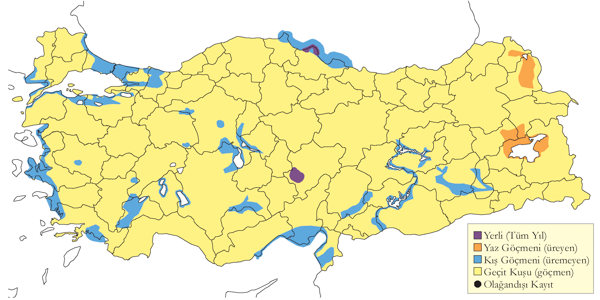
\includegraphics{images/harita_Page_017.png}

\textbf{Üreme}

\textbf{Yuvalama alanı}: Büyük sulakalanlarda yuvalar.\\
\textbf{Yuvası}: Kulu Gölü'nde bir adadaki seyrek bitki örtüsü içinde
yuvalamıştır. Yuvasını çıplak zeminde sığ bir oyuk açarak yapar ve içine
ot, bitki gövdeleri ve tüylerini karıştırarak döşer.\\
\textbf{Yumurta sayısı}: 8-10 yumurta bıraktığı kaydedilmiştir.\\
\textbf{Üreme Dönemi:} Türkiye'deki üreme sezonu hakkında yeterli veri
bulunmamaktadır; diğer ülkelerde ise üreme sezonu genellikle nisan başı
ile mayıs sonu arasındadır.\\
\textbf{Karadeniz:} 6-7 Temmuz 1972'de Kızılırmak Deltası'nda dört ve
beş yavrulu iki dişi kaydedilmiştir (Dijksen \& Kasparek 1985). 1992
yılında üreme kanıtlanamamış ve popülasyonun 0-1 çift olduğu
belirtilmiştir (Hustings \& Dijk 1994). 1971 yılı Temmuz ortasında
kaydedilen yumurtalı yuvalar, başarısız bir üremenin ardından
gerçekleşen ikinci bir üreme denemesi olarak değerlendirilmiştir.\\
\textbf{İç Anadolu:} 14-15 Temmuz 1971'de Kulu Gölü'ndeki bir adada
sekiz ve on yumurtalı iki yuva tespit edilmiştir. 5-6 Ağustos 1972'de
iki ve dört yavrulu iki yavru grubu gözlenmiştir (Kasparek 1987). 31
Mayıs 1987'de Kulu Gölü'nde yavrular gözlenmiş, 19 Haziran 1992'de dokuz
yumurtalı bir yuva bulunmuştur. Haziran 1977'de Eşmekaya'da beş
yavrusuyla birlikte bir dişi gözlenmiştir (Schubert 1979).\\
\textbf{Doğu Anadolu:} 29 Mayıs 1969'da Van Gölü'nde kur davranışı
gözlenmiştir.

\textbf{Alttürler ve Sınıflandırma}

Monotipik bir türdür.

\section{Kılkuyruk}\label{kux131lkuyruk}

\emph{Anas acuta}, Northern Pintail

\textbf{Nispeten yaygın olarak bulunan bir geçit türü ve kış konuğudur.
Nadiren yuvalar.}

Son yıllarda 1998 ve 1999'da, tek bir alanda, Girdev Gölü'nde üremiştir.
İlkbaharda ve yazın İç Anadolu'da birçok erişkin kaydı olsa da,
kanıtlanmış üreme kayıtları az sayıdadır. Üreyen popülasyonun 500 ile
1000 çift olması iddiası tamamen geçersizdir (Tucker \& Heath 1994).

Genellikle eylül ortasından nisan başına kadar batı ve orta bölgelerde
görülür.

Ülke genelinde kışlayan nüfus 10.000 bireyden azdır. 1986'da toplam
25.700 birey, 1992'de 11.070 birey ve 1999'da 13.573 birey kışlamıştır.
Kışlama popülasyonunda çarpıcı bir azalma belgelenmiştir. 60'li yıllarda
düzenli olarak 100.000'in üzerinde sayılırdı. Örneğin, 1967'de Büyük
Menderes Deltası'nda 60.000 birey, Emir Gölü'nde 70.000 birey, 1969'da
Akyatan Gölü'nde 100.000 birey ve Gâvur Gölü'nde 50.000 birey
kaydedilmiştir. Bilhassa ılıman geçen kışlarda daha yüksek sayılarda
kaydedilebilir. Eski tarihlerde bazı alanlardaki sayımların sonuçlarının
güvenilirliği sorgulanabilir, örneğin, 1970'de Sultansazlığı'ndaki
sayılan 160.000 birey muhtemelen abartılı bir tahmindir. Bu ve diğer
ördek türlerinin önemli sayılarda kışladığı birkaç sulakalan kısmen ya
da tamamen kurutulmuş durumdadır. Diğer yandan son yıllarda oluşan baraj
göllerinde kışlamaya başlamıştır.

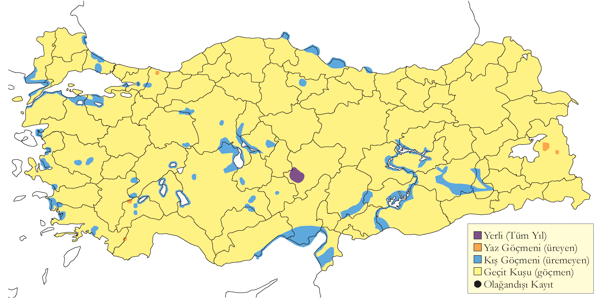
\includegraphics{images/harita_Page_018.png}

\textbf{Üreme}

\textbf{Yuvalama alanı}: Büyük göllerde ve sulakalanlarda yuvalar.\\
\textbf{Yuvası}: Kulu Gölü'ndeki büyük adada kıyı vejetasyonu içinde
yuvalamıştır. Yerdeki bir delikte yaptığı yuvasını bitkisel malzemeler,
hav tüyleri ve kontür tüyleri ile kaplanmıştır.\\
\textbf{Yumurta sayısı}: 6-10 yumurta koyduğu kaydedilmiştir.\\
\textbf{Üreme dönemi}: Görünüşe göre mayıs ayında yumurtlar.
\textbf{KAR.} Kızılırmak Deltası'nda üreme davranışları gözlenmiş,
ürediği kesinleşmemiştir (Hustings \& Dijk 1994). \textbf{AKD.} Haziran
1998 ve 1999'da Girdev Gölü'nde yavrular gözlenmiştir. \textbf{İÇA.} 22
Mayıs 1992'de Kulu Gölü'nde yedi ve on yumurtalı iki yuva, 19 Haziran
1992'de 6 ila 9 yumurtalı beş yuva bulunmuştur. 24 Haziran 1992'de
Bolluk Gölü'ndeki bir çalının altına gizlenen yuvada 11 yumurta
sayılmıştır.

\textbf{Alttürler ve Sınıflandırma}

Türkiye'de nominat alttürü bulunur.

\section{Çıkrıkçın}\label{uxe7ux131krux131kuxe7ux131n}

\emph{Spatula querquedula}, Garganey

\textbf{Yaygın olarak az sayıda üreyen bir yaz göçmenidir. Bunun yanında
göç döneminde daha yaygın ve çok sayıdadır. Nadiren kışlar.}

Ördeklerin arasında esasen yaz göçmen olan tek türdür. Şubat ortasından
itibaren görülmeye başlar, ekim sonuna kadar kalır. Leylekle beraber en
erken gelen göçmen kuşlardandır. Sazlık sulakalanları tercih eder, en
yoğun ürediği alanlar İç ve Doğu Anadolu'dadır. Güneydoğu Anadolu'da iki
alanda üremesi olasıdır.

İlkbahar ve sonbahar boyunca Türkiye'nin tüm bölgelerinde yüzlerce,
hatta binlerce birey sürüler halinde gözlenebilir. İlkbahar geçişi şubat
sonundan mayıs sonuna kadar devam eder. Sonbahar geçişinde ise ağustos
sonu ile eylül başı arasında Karadeniz kıyıları boyunca göçmen sürülere
rastlanabilir.

Nadiren Marmara, Ege ve Akdeniz'de az sayıda kışlar. Olağandışı yumuşak
geçen 1968-69 kışında Göksu Deltası'nda 3000 birey ve Gâvur Gölü'nde
5000 birey sayılmıştır. Güncel tarihlerde; Ocak 2002'de Güllük
Deltası'nda 65 birey, Şubat 2002'de Bafa Gölü'nde 58 birey, Aralık
2002'de Çukurova'da 89 birey, 4 Aralık 2010'de Karkamış Barajı'nda iki
birey kışlamıştır.

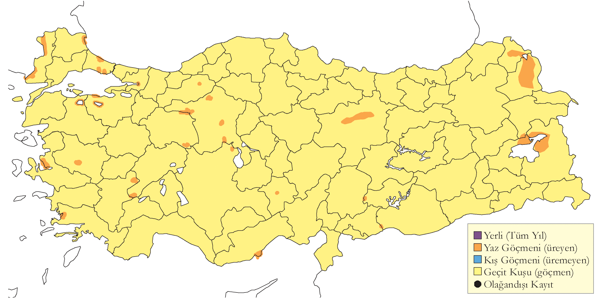
\includegraphics{images/harita_Page_019.png}

\textbf{Üreme}

\textbf{Yuvalama alanı}: Sazlık sulakalanlarda yuvalar.\\
\textbf{Yuvası}: Göl kenarlarındaki ıslak çayırlar, bataklıklar ve
sazlıklarda, ikisinin bir arada olduğu alanlarda ve göl kenarındaki
vejetasyonun içinde ürer.\\
\textbf{Yumurta sayısı}: Türkiye'den veri yoktur, diğer yerlerde olağan
yumurta sayısı 8-11'dir.\\
\textbf{Üreme dönemi}: Nisan ortasından itibaren ürer. Yavrular temmuza
kadar görülebilir. \textbf{KAR.} 19 Mayıs 1992'de Yeniçağa Gölü'nde yeni
bozulmuş ancak yumurtaların taze olduğu açıkça anlaşılan iki yuva, 6
Mayıs 1993'te yakınlardaki ıslak bir çayırlıkta bir yuva bulunmuştur. 13
Mayıs 1986'da Abant Gölü'nde 17 yavru ve bir dişi gözlenmiş, yumurtlama
tarihinin nisan ortası civarında olduğunu hesaplanmıştır. 2 Ağustos
1971'de Kızılırmak Deltası'nda bir çift ve yedi yavru kaydedilmiştir.
\textbf{İÇA.} 10-15 Mayıs 1991'de Hotamış Sazlığı'nda yavrulu birkaç
çift gözlenmiş (Kirwan 1993a), 27 Temmuz 1971'de Kulu Gölü'nde büyük
yavruları olan altı çift kaydedilmiş, Haziran ve Temmuz 1968'de Mogan
Gölü'nde 1-2 kuluçka gözlenmiş, 27 Temmuz 1971'de Yarma'da büyük
yavruları olan en az dört çift tespit edilmiştir.

\textbf{Alttürler ve Sınıflandırma}

Monotipik bir türdür.

\section{Çamurcun}\label{uxe7amurcun}

\emph{Anas crecca}, Eurasian Teal

\textbf{\emph{Lokal olarak az sayıda ürer. Bunun yanında yaygın olarak
ve çok sayıda bulunan kış konuğudur.}}

İç Anadolu, Doğu Anadolu ve Kızılırmak Deltası'nda yuvalar. Kızılırmak
Deltası'nda 1992'de 15-20 çift üremiştir (Hustings \& Dijk 1994), Doğu
Anadolu'dan teyit edilmiş üreme kaydı ise çok azdır.

Geçiş sırasında eylül başından nisan başına kadar ülkenin batı ve orta
bölgelerinde yaygın olarak çok sayıda görülebilir. Marmara ve Karadeniz
bölgelerinde ara sıra yüksek sayılarda kaydedilebilir.

Kışın hem iç bölgelerde hem de kıyısal sulakalanlarda yüksek sayıda
bulunur. Ülke çapında kışlayan nüfus 100.000 birey seviyesindedir. Son
yıllarda kışlayan nüfusta düşüşler yaşanmış, örneğin 1988'de 21.000
birey ve 1989'da 13.400 birey sayılmıştır. Bu düşüş, aslında diğer yüzey
ördeklerinde olduğu gibi 1960'lardan beri süre gelmektedir. 1968-69'da
toplam 270.400 birey ve 1969-70'de 326.700 birey sayılmıştır. Son
sayımda sadece Sultansazlığı'nda 200.000 birey gözlenmiştir. Alanda
sayılan ancak türü tespit edilemeyen 400.000 ördeğin de çamurcun
olabileceği düşünülürse, alandaki kışlayan çamurcun sayısı 600.000 birey
olabilir.

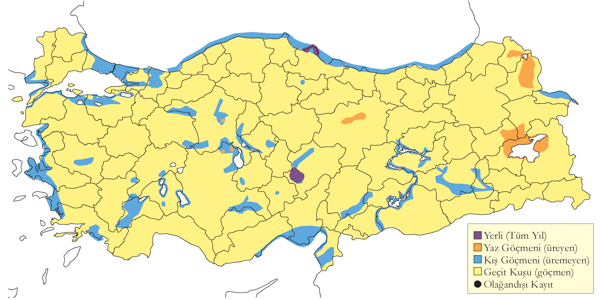
\includegraphics{images/harita_Page_020.png}

\textbf{Üreme}

\textbf{Yuvalama alanı}: Göllerde ve sazlıklarda ürer.\\
\textbf{Yuvası}: Yuva ve yumurta sayısı Türkiye'den bilinmez. Diğer
yerlerde yuvasını yerdeki bir oyuğa yapar ve genellikle yapraklar,
bitkisel malzemeler, hav tüyleri ve kontur tüyleriyle kaplar.
Sulakalanlarda yüksek otların üzerine yuvalar, nadiren sudan uzağa da
yuva yapabilir.\\
\textbf{Yumurta sayısı}: Türkiye'den veri yoktur, ancak diğer yerlerde
olağan yumurta sayısı 8-12'dir.\\
\textbf{Üreme dönemi}: Nisan ortasından itibaren ürer, yavrular temmuza
kadar görülebilir. \textbf{KAR:} 29 Mayıs 1979'da Kızılırmak Deltası'nda
içinde yumurta olan bir yuva bulunmuş, 28 Temmuz 1971'de dokuz yavrulu
bir dişi ve 6 Ağustos 1971'de beş yavrulu bir dişi gözlenmiştir (Dijksen
\& Kasparek 1985). 1992'de popülasyonun 15-20 çift olduğu belirlenmiş, 5
Mayıs'ta dikkati başka yere çekme davranışı gözlenmiş ancak hiçbir yuva
bulunamamıştır (Hustings \& Dijk 1994). \textbf{İÇA}: 14 Mayıs 1991'de
Hotamış Sazlığı'nda yavrularıyla birlikte birkaç erişkin gözlenmiş, bu
da yumurtaların en geç nisan ortasında koyulmuş olduğunu göstermiştir
(Kirwan 1993a). 5-6 Ağustos 1972'de Kulu Gölü'nde iki dişinin 7 ve 10
yavrusu gözlenmiştir (Kasparek 1987). \textbf{DOA}: 24 Haziran 1983'te
Haçlı Gölü'nde tek yavrulu bir dişi kaydedilmiştir.

\textbf{Alttürler ve Sınıflandırma}

Türkiye'de nominat alttürü bulunur.

\section{Yaz Ördeği}\label{yaz-uxf6rdeux11fi}

\emph{Marmaronetta angustirostris}, Marbled Duck

\textbf{\emph{Türkiye'de üreyen nüfus yok olmuştur.}}

Göksu Deltası'nda üreyen popülasyonun 2013 yılından sonra yok olmasıyla,
üreyen tür olarak Türkiye'deki soyunun tükendiği söylenebilir. Tek tük
Doğu Akdeniz, Güneydoğu ve Doğu Anadolu'da görülebilir. Marmara, Ege ve
Karadeniz bölgelerinde eski tarihli kayıtları vardır. En yakın üreme
alanı Irak'taki Mezopotamya Bataklıkları'dır.

Mart başından ekim başına kadar kaydedilen bir yaz konuğu idi. Göksu
Deltası'ndaki üreyen popülasyon, 1989 ile 2013 arasında adım adım
azalmıştır. 1989 ve 1991'de yaklaşık 50 çift tespit edilmiş, 2000'li
yıllarda bu sayı 10 çifte düşmüş, 2010 ile 2013 arasında sadece 1 ila 2
çift kalmış ve 2014 yılından itibaren alanda görülmemeye başlamıştır. Bu
nedenle Türkiye'de üreyen nüfusunun yok olduğu kabul edilmiş (Boyla et
al. 2018) ve Yaz Ördeği, Yılanboyun'dan sonra Türkiye'de soyu tükendiği
belgelenen ilk kuş türü olmuştur.

1987 yılında Çukurova'da, bugün yok edilmiş olan Dipsiz Gölü'nde 32 çift
tespit edilmiştir. İç Anadolu'da Ereğli Sazlığı'nda muhtemelen 1-4 çift,
Hotamış Sazlığı'nda 10-15 çift ve Sultansazlığı'nda 1-4 çift üremiştir.
Van Gölü havzasında ise Erciş Gölü ve Van Sazlığı'nda az sayıda ürediği
teyit edilmiş, bunun yanında Ağrı çevresi, Ahlat Sazlıkları, Bendimahi
Deltası ve Kuyucuk Gölü'nde üreme döneminde görülmüştür. 1987 yılında
ülke nüfusunun 50-100 çift olduğu düşünülmüştür. Üreme sonrasında
Çukurova ve Göksu Deltası'nda 100-200 bireyin toplandığı bilinir.
Nadiren az sayıda kışlamıştır. En son sayımlarda 1993'te Çukurova'da
dört, 1997'de aynı alanda 35 birey sayılmıştır.

Amik Gölü'nün kurutulmasından önce muhtemelen önemli sayılarda
bulunuyordu (Kumerloeve 1963a). Konya havzasındaki Yarma Sazlıkları,
Gönenç Gölü ve Karapınar Ovası'nda (Grimmett \& Jones 1989) muhtemelen
üremiştir. Mogan Gölü ve Eber Gölü gibi diğer birkaç alanda da üremiş
olabilir. Bu alanlar ekolojik özelliklerini kaybettikleri ve türe uygun
üreme habitatları barındırmadıkları için artık üremeye elverişli
değildir. Üreme sonrası toplanan bireyler, o yıllarda toplam ülke nüfusu
hakkında fikir verebilir. Ağustos 1967'de Çukurova'da 2000 birey ve
Göksu Deltası'nda 450 birey sayılmıştır.

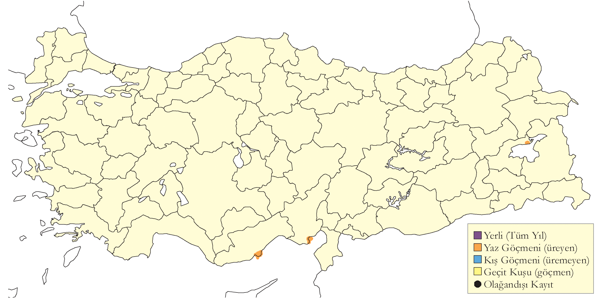
\includegraphics{images/harita_Page_021.png}

\textbf{Üreme}

\textbf{Yuvalama Alanı:} Çukurova ve Göksu Deltası'nda sığ ve ötrofik
göllerde bulunmuştur. Genellikle sazlık adaların, bitişik havuzlar ve
sazlıkların bulunduğu yoğun sualtı vejetasyonuna sahip sığ göllerin
çevresinde ürer ve geniş sulakalanları tercih eder. Sanılanın aksine acı
veya tuzlu sularda değil tatlı suları tercih eder.\\
\textbf{Yuvası:} 9 Haziran 1993'te Göksu'da, kofanın (\emph{Juncus})
baskın olduğu ve yakınlarda sazların (\emph{Phragmites}) da bulunduğu
bataklık bir bölgede sığ gölcüklerin olduğu bir alanda, yaklaşık 1 m
çapındaki bir \emph{Juncus} kümesinin içinde, sudan yaklaşık 0,7 m
yüksekte gizlenmiş iki yumurtalı bir yuva bulunmuştur. Yuva sazlardan ve
bitki gövdelerinden yapılmış dayanıklı bir kâse şeklindedir ve ince
bitkisel malzemeyle kaplanmıştır; hav tüyü kullanılmamıştır.\\
\textbf{Yumurta Sayısı:} Yumurta sayısı 2 ile 12 arasında değişir,
ortalama 6,5 yumurta olarak hesaplanmıştır (Green 1993). Diğer
bölgelerde ise tipik yumurta sayısı 9-13'tür (5-18).\\
\textbf{Üreme Dönemi:} 22 Mayıs 1971'de Çukurova'da kaydedilen altı
yavru, en erken kayıttır ve yumurtlamanın nisanın ikinci yarısında
başladığını gösterir. Ana yumurtlama dönemi, mayısın ikinci yarısıyla
haziran başı arasındadır. Yavrular en erken 7 Haziran'da ortaya çıkar ve
temmuz sonuna kadar küçük yavrular görülebilir. Tamamen palazlanmış
yavrular temmuz başında kaydedilmiştir. \textbf{AKD:} 1991'de Göksu
Deltası'nda yaklaşık 50 çiftten en az 31'i yavru çıkarmıştır. Aynı yıl
Göksu Deltası'nda 11 yuvada 8-13, 5 yuvada 4-6 ve bir yuvada 15 yavru
sayılmıştır. 15 yavrunun, iki dişinin yumurtalarının bir araya
gelmesiyle oluştuğu düşünülmektedir. Benzer şekilde 15-18 Temmuz 1992'de
bir dişi 32 yavruyla görülmüştür (Green 1993). 10 Temmuz 1967'de hem
büyük hem küçük yavrular haziran ve temmuzda az sayıda gözlenmiştir
(Vielliard 1968). \textbf{İÇA:} 4-5 Haziran 1971'de Yarma Sazlığı'nda 6
ve 13 yumurtalı iki yuva bulunmuş, bir yuvada bir Yeşilbaş yumurtası
görülmüştür. 12 Haziran 1998'de Kulu Gölü'nde tek yavrulu bir erişkin
kaydedilmiş ve temmuz ayında üç farklı alanda yavrular gözlenmiştir.
\textbf{DOA:} 22 Temmuz 1987'de Van Sazlığı'nda küçük yavruları olan iki
çift gözlenmiş, bu gözleme dayanarak yumurtlamanın haziran ortasında
olduğu tahmin edilmiştir. Aynı alanda temmuz sonunda ve ağustos başında
genç bireyler kaydedilmiştir.

\textbf{Alttürler ve Sınıflandırma}

Monotipik bir türdür.

\section{Macar Ördeği}\label{macar-uxf6rdeux11fi}

\emph{Netta rufina}, Red-crested Pochard

\textbf{\emph{Lokal olarak nispeten çok sayıda ürer. Kışın daha
yaygındır ve bazı alanlarda yüksek sayılarda toplanır.}}

İç Anadolu'daki geniş sodalı ya da tatlı sazlık sulakalanlarda çok
sayıda ürer. Sultansazlığı'nda yüksek sayılarda bulunur. 1990'larda
Ereğli Sazlığı'nda 500 çift üremişken 1998'de sadece 20 çift üremiş,
alanın kurutulmasıyla buradan tamamen yok olmuştur. Kızılırmak
Deltası'nda 1992'de 50-75 çift üremiştir (Hustings \& Dijk 1994). Diğer
alanlarda nispeten yüksek sayılarda yuvalayanlar yerli veya yarı
göçmendir. Çukurova sulakalanları ve Göksu Deltası'nda üreyen nüfus
1990'dan sonra azalmıştır. Türkiye'de üreyen popülasyon 1000-5000 çift
olarak tahmin edilmiştir (Tucker \& Heath 1994). Son yıllarda İç
Anadolu'da üreyen kuşların sayılarında yaşanan azalma, güncel ulusal
nüfusun çok daha az olduğuna işaret etmektedir.

Ülke genelinde geçiş sırasında doğu bölgeleri dışında daha yaygındır.
Çoğu zaman yüzeyi donmaya daha az eğilimli olan baraj göllerini tercih
eder. Ocak 1967'de 12.000 birey sayılmış, bunun 7000'i bugün kurutulmuş
olan Amik Gölü'ndendir. Türkiye genelinde 1992'de 5249, 1996'da 6522 ve
1999'da 6228 birey sayılmıştır. 2000'li yıllarda toplam sayıda artış
görülmüş, sadece Beyşehir Gölü'nde Şubat 2003'te 10.000 birey ve Ocak
2005'te 20.000 birey sayılmış, son sayımda hem toplam hem de alan rekoru
kırılmıştır.

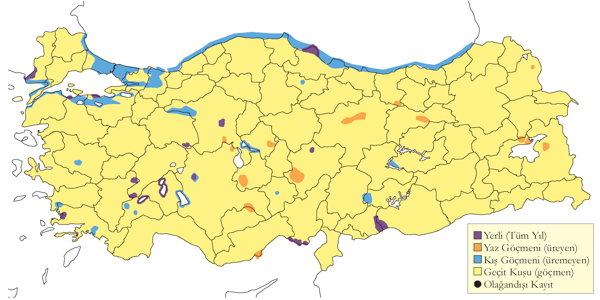
\includegraphics{images/harita_Page_022.png}

\textbf{Üreme}

\textbf{Yuvalama Alanı:} Yoğun sazlıkların ve su kenarı bitkilerinin
bulunduğu tatlı ya da sodalı göllerde ve su aynalarına sahip sazlıklarda
ürer.

\textbf{Yuvası:} Yerdeki bir oyuğa yaptığı yuvasını bitkisel malzeme,
hav tüyleri ve tüylerle kaplar. Çoğunlukla yoğun vejetasyonun içine,
nadiren açıkta (örneğin adalarda) ya da nemli alanlarda su seviyesinin
üzerindeki saz öbeklerinin ya da diğer sucul bitkilerin içine genellikle
iyice gizlenmiş bir yuva yapar.

\textbf{Yumurta Sayısı:} Türkiye'de gözlenen yumurta sayısı 4-12 olup,
ortalama 8,3'tür (18 yuvada). Bir yuvada bulunan 24 yumurta muhtemelen
birden fazla dişiye aittir. Yavru sayısı 2-12 arasında değişir ve 16
yuvada ortalama 6,2'dir. Sadece 2-4 yavru çıkarabilmiş 6 dişi ortalamayı
düşürmüştür.

\textbf{Üreme Dönemi:} Nisan sonu ile temmuz başı arasında yumurtlar.
Yavrular temmuz sonuna kadar görülebilir. \textbf{MAR:} 1 Mayıs 1993'te
Kocaçay Deltası'nda yumurtalı bir yuva bulunmuştur (Ertan 1996).
\textbf{KAR:} Kızılırmak Deltası'nda 27 Mayıs 1992'de beş yumurtalı bir
yuva bulunmuş, 4 Haziran 1992'de yaklaşık bir haftalık ilk tüylü yavru
kaydedilmiş (Hustings \& Dijk 1994) ve 27 Mayıs 1979'da sekiz yavrulu
bir aile gözlenmiştir (Dijksen \& Kasparek 1985). \textbf{AKD:} 18
Temmuz 1992'de Karamık Gölü'nde küçük yavrulardan oluşan bir aile
gözlenmiştir. \textbf{İÇA:} Çoğu mayısta olmak üzere 25 Nisan'da yumurta
kayıtları vardır. En geç kayıt 19 Haziran 1992'de 12 yumurtalı bir
yuvadır. Biri 11 Mayıs'ta, çoğu haziranda olan birçok yavru kaydı
vardır, en geç 8 Temmuz 1967'de (Vielliard 1968) ve 5 Ağustos 1972'de
küçük yavrular gözlenmiştir. \textbf{DOA:} 21-22 Temmuz 1986'da Van
Gölü'nde 7-8 yavrulu üç yavrulu bir aile kaydedilmiştir.

\textbf{Alttürler ve Sınıflandırma}

Monotipik bir türdür.

\section{Elmabaş Patka}\label{elmabaux15f-patka}

\emph{Aythya ferina}, Common Pochard

\textbf{Nispeten yaygın ve çok sayıda bulunan yerli ve yarı göçmen,
yaygın ve çok sayıda bulunan kış konuğudur.}

İç ve Doğu Anadolu'daki sulakalanlarda orta sayılarda üreyen yerli ve
yarı göçmendir. 1992'de Kızılırmak Deltası'nda 300-350 çiftin ürediği
tahmin edilmiştir (Hustings \& Dijk 1994). Uygun habitatların azlığı
nedeniyle Karadeniz, Güneydoğu Anadolu ve diğer bölgelerde lokal olarak
bulunur. Muhtemelen gerçek üreme durumunu çarpıtacak şekilde, hatırı
sayılır sayıda üremeyen birey özellikle İç ve Doğu Anadolu'da yazı
geçirir.

Kışın ve geçiş dönemlerinde ülke genelinde yaygın ve boldur. Son
yıllarda ortalama 67.000 bireyden fazla sayılmaktadır. 1996 yılında
Beyşehir Gölü'nde 47.000, Uluabat Gölü'nde 42.000 ve ülke genelinde
toplamda 250.000 birey sayılmıştır, bu en yüksek kayıtlardandır. 1999'da
Eğirdir Gölü'nde 40.000, ülke genelinde ise 137.000 kuş sayılmıştır. 18
yıllık Kış Ortası Su kuşu sayımlarının ortalaması 93.000 kuştur. İstisna
olarak 1968-69 kışında 355.000 bireyin kışladığı tahmin edilmiştir. Ekim
ortasından itibaren yüksek sayılar gözlemlenir; Göksu Deltası'nda Ekim
1978'de 40.000, Ekim 2002'de Sodalıgöl'de 100-130.000, Kulu Gölü'nde
Kasım 1970'de 45.000 ve Kasım 1971'de 28.000 birey kaydedilmiştir.

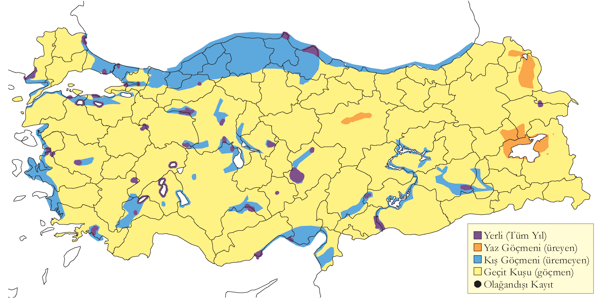
\includegraphics{images/harita_Page_023.png}

\textbf{Üreme}

\textbf{Yuvalama alanı}: Göl kıyılarındaki sazlıklarda ve su aynalarının
bulunduğu sazlık bataklıklarda ürer.\\
\textbf{Yuvası:} 19 Haziran 1984'te Erçek Gölü yakınlarındaki küçük bir
gölde, sık bir örtü içindeki sazların dibine tutturulmuş ve sakarmeke
yuvasına benzer şekilde sudan yükseğe yapılmış bir yuva bulunmuştur.
Yuva, ölü saz gövdeleri ve diğer bitkisel malzemelerle derin ve düzgün
bir kâse şeklinde örülmüş, bol miktarda hav tüyü ve diğer tüylerle
kaplanmış dayanıklı bir yapıya sahiptir. Diğer bölgelerdeki yuvalar da
genellikle benzer alanlarda olup nadiren su kıyısındaki yoğun bitki
örtüsünün içinde kuru zeminde de bulunabilir.\\
\textbf{Yumurta Sayısı:} Türkiye'de yumurta sayısı kaydedilmemiştir,
ancak gözlenen yavru sayısından 8-11 yumurta bırakabileceği
düşünülmektedir. Diğer bölgelerde genellikle 6-9 yumurta bırakır.
Gözlenen yavru sayısı ortalama 6,6'dır.\\
\textbf{Üreme Dönemi:} Nisan başı ile haziran ortasına kadar yumurta
bırakır. Yavrular temmuz ayında gözlenebilir. \textbf{KAR}. Kızılırmak
Deltası'nda 11 Mayıs 1992'de hav tüyleriyle kaplı birkaç günlük yavru,
en erken kayıt olarak görülmüş ve bu da yumurtlamanın nisanın ilk
haftasında olduğunu göstermiştir (Hustings \& Dijk 1994). 14 Haziran
1984'te yaklaşık 5 günlük yavrulardan oluşan bir kuluçka ile yaklaşık üç
haftalık yavrulardan oluşan iki kuluçka gözlenmiştir (Dijksen \&
Kasparek 1985). \textbf{İÇA}. Haziran başlarında iki yumurtalı
(tamamlanmamış) bir yuva bulunmuş, Haziran 1971'de Boz Ördek yuvalarına
iki, dört ve beş yumurta bırakıldığı tespit edilmiştir. 13 Mayıs 1991'de
Hotamış'ta yumurtalı bir yuva bulunmuştur (Kirwan 1993a). 1970 yılının
mayıs ayı sonunda Eşmekaya'da küçük yavrulardan oluşan beş yavru, 1
Haziran 1969'da Sultansazlığı'nda altı yavru ve haziran-temmuz aylarında
diğer alanlarda yavrular gözlenmiştir. \textbf{DOA}. 19 Haziran 1983'te
Van Sazlığı'nda yavrularıyla birlikte sekiz dişi kaydedilmiştir.

\textbf{Alttürler ve Sınıflandırma}

Monotipik bir türdür.

\section{Pasbaş Patka}\label{pasbaux15f-patka}

\emph{Aythya nyroca}, Ferruginous Duck

\textbf{Lokal olarak az sayıda üreyen yaz konuğu, yaygın ve nispeten çok
sayıda bulunan geçit türü, yaygın ancak az sayıda kış konuğudur.}

Tüm bölgelerdeki sulakalanlarda oldukça lokal bir yaz konuğudur. En
yüksek sayılarda İç ve Doğu Anadolu bölgelerinde bulunur. Kızılırmak
Deltası (1992'de tahminen 150-200 çift (Hustings \& Dijk 1994)), Kocaçay
Deltası (1993'te tahminen 70 çift (Ertan 1996)), Uluabat Gölü (1988'de
tahminen 32 çift (Welch \& Welch 1998b)) ve Göksu Deltası (yaklaşık 30
çift) önemli sayılarda ürediği alanlardır. Son yıllarda gerçekleştirilen
çalışmalarda Güneydoğu Anadolu'da üç yeni üreme alanı belirlenmiştir.
Yaz göçmenleri mart ortasından eylül sonuna kadar gözlenir.

Türkiye popülasyonu muhtemelen dünyadaki en önemlilerinden biridir ve
1000 ile 3000 çift arasında olduğu düşünülmüş (Tucker \& Heath 1994),
sonra bu tahmin 500-600 çift olarak güncellenmiştir (Kirwan 1997a).
Avrupa'da yayılış alanının bir kısmında yaşanan sert düşüş dikkate
alındığında, Türkiye popülasyonunun izlenmesine acil ihtiyaç
duyulmaktadır. 1990'ların sonlarında İç Anadolu'daki birkaç alanda da
azalma görülmüştür.

Geçiş sırasında az ve orta sayılarda bulunur ve ülke genelinde biraz
daha yaygındır. Az sayıda kışlar, 1992 yılında 105 birey, diğer yıllarda
50 bireyden az sayılmıştır. 1990'ların ortalarından itibaren kış
kayıtlarında bir artış gözlenmiş, bu durum muhtemelen gözlemci sayısının
artmasına bağlanmıştır. Eskiden batı ve orta bölgelerde daha çok sayıda
kışlamış, 1968-74 yıllarında 50 ile 450 birey arasında kaydedilmiştir.
Marmara Gölü'nde kaydedilen 860 birey en yüksek kayıttır. Doğu ve
Güneydoğu Anadolu'da 2005 yılında sayılan 44 birey bahsedilmeye
değerdir.

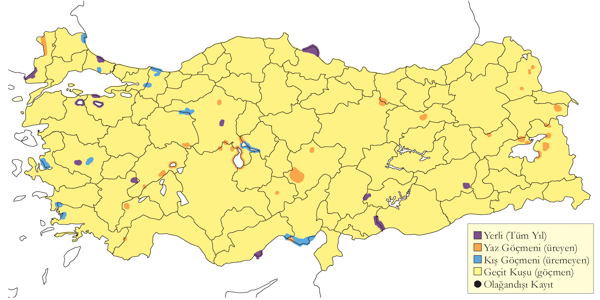
\includegraphics{images/harita_Page_024.png}

\textbf{Üreme}

\textbf{Yuvalama Alanı:} Çevresinde sazlıkların, yoğun su üstü
vejetasyonunun ve çoğunlukla daha geniş sazlıkların ve bataklıkların
bulunduğu tatlı su göllerinde ürer.\\
\textbf{Yuvası:} Su kenarındaki yoğun vejetasyonun içine yuva yapar.
Kulu Gölü'ndeki bir adada, alçak çalıların arasında çıplak zeminde hafif
bir çukurun içine yapılan yuvanın ot ve hav tüyleriyle kaplandığı
gözlenmiştir ((Pforr \& Limbrunner 1982); A. Limbrunner, kişisel
görüşme).\\
\textbf{Yumurta Sayısı:} Türkiye'de gözlenen yumurta sayısı 6-8
arasındadır.\\
\textbf{Üreme Dönemi:} Nisan ile haziran başı arasında yumurta bırakır.
Yavrular ağustos ayına kadar gözlenebilir. \textbf{MAR.} 19 Haziran
1999'da Uluabat Gölü'nde bazıları küçük yavrulardan oluşan birkaç yavru
grubu gözlenmiş, 1966'da Manyas Gölü'nde de yavrular kaydedilmiştir.
\textbf{KAR.} Kızılırmak Deltası'nda çiftlerin çoğu sazlık alanlarda
gözlenmiştir. 5 Mayıs 1992'de altı yumurtalı bir yuva bulunmuş ve 1
Haziran 1992'de yumurtlamanın nisan sonlarından daha geç olmadığını
gösteren üç ve dört yavrulu iki grup kaydedilmiştir (Hustings \& Dijk
1994). 6 Ağustos 1971'de yedi yavrulu bir grup gözlenmiştir.
\textbf{AKD.} 15 Mayıs 1962'de Çukurova'da sekiz yumurtalı bir yuva
(Kirwan 1997a), 8 Mayıs 1953'te Amik Gölü'nde yumurtalı bir yuva (Kirwan
1997a), ve 27 Mayıs 1933'te yumurta kanalında yumurta bulunan bir dişi
vurulmuştur (Meinertzhagen 1935). Göksu Deltası'nda en erken 17
Haziran'da olmak üzere yedi yuva alanında yavrular gözlenmiştir.
\textbf{İÇA.} 28 Nisan 1982'de Sultansazlığı'nda yumurtalı bir yuva
bulunmuştur (Kirwan 1997a). Mayıs 1973'te Kulu Gölü'nde altı yumurtalı
bir yuva bulunmuştur. En erken 20 Haziran'da Eber Gölü'nde olmak üzere
Çöl Gölü, Gönenç Gölü, Sultansazlığı, Mogan Gölü ve Kulu Gölü'nde
yavrular gözlenmiştir. \textbf{DOA.} Yumurtlamanın mayıs sonunda
olduğunu gösteren gözlemler 1985 ve 1987 yıllarında haziran sonunda Van
Gölü'nde ve 29 Haziran 1987'de Edremit Sazlığı'nda yapılmıştır (Kirwan
1997a).

\textbf{Alttürler ve Sınıflandırma}

Monotipik bir türdür.

\section{Tepeli Patka}\label{tepeli-patka}

\emph{Aythya fuligula}, Tufted Duck

\textbf{\emph{Lokal ve az sayıda üreyen yaz konuğu, nispeten yaygın ve
çok sayıda bulunan kış konuğudur.}}

Çok nadir ve lokal olarak üremiştir. Kızılırmak Deltası'nda ve 1967 ile
1981'de Çalı Gölü'nde (Kars) ürediği kanıtlanmış, son alanda 20 çiftlik
bir popülasyon tespit edilmiştir. Başka bölgelerde düzenli olarak yazı
geçirir. Uluabat Gölü ve Uyuz Gölü gibi bazı alanlardaki uygun
habitatlarda çiftler gözlenmiştir. Üreme sonrasında, Temmuz 1982'de Kulu
Gölü'nde tüy değişimi için toplandıkları düşünülen 700 birey (Kasparek
1987), Eylül 1967'de ise Sodalı Gölü'nde çoğu erkek olan 1200 birey
sayılmıştır.

Ülkenin batı ve orta bölgelerinde eylül başından nisan başına kadar
kaydedilen yaygın ve bol bulunan bir geçiş türü ve kış konuğudur.
Karadeniz'de denizde kışlar. Kış ortası sayımlarında; 1968-69 kışında
20.800 birey, 1996'da en yüksek sayı olan 58.271 birey, 1992'de yaklaşık
13.000 birey, 1993'te 16.965 birey (sadece Eğirdir Gölü'nde 10.478
birey) ve 1999'da 18.512 birey kaydedilmiştir. Son yıllarda ise ülke
toplamı genellikle 5000-10.000 birey arasındadır. En önemli kışlama
alanları Sapanca Gölü ve Eğirdir Gölü'dür.

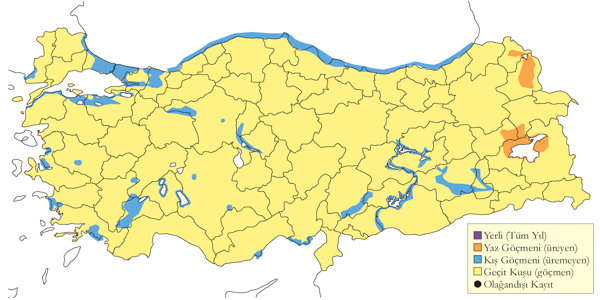
\includegraphics{images/harita_Page_025.png}

\textbf{Üreme}

\textbf{Yuvalama alanı}: Su üstü vejetasyonu olan tatlı su göllerinde
ürer.\\
\textbf{Yuvası}: Yuvasını bir bitki öbeğinin altına kurar.\\
\textbf{Yumurta sayısı}: Türkiye'de 8 yumurtalı bir yuva bulunmuştur.\\
\textbf{Üreme dönemi}: Mayıs ayında yumurta koyar, temmuz sonuna kadar
yavrular görülebilir. \textbf{KAR.} Kızılırmak Deltası'nda, 5 Mayıs
1992'de sazlıkta bir \emph{Juncus acutus} öbeğinin dibinde sekiz
yumurtalı bir yuva bulunmuş (Hustings \& Dijk 1994) ve 28 Mayıs 1968'de
de ürediği kanıtlanmıştır (Dijksen \& Kasparek 1985). \textbf{DOA.} Çalı
Gölü'nde 19 Temmuz 1992'de yavrularıyla birlikte iki dişi gözlenmiştir
(Magnin \& Yarar 1997).

\textbf{Alttürler ve Sınıflandırma}

Monotipik bir türdür.

\section{Karabaş Patka}\label{karabaux15f-patka}

\emph{Aythya marila}, Greater Scaup

\textbf{\emph{Özellikle Karadeniz kıyılarında az sayıda ve düzenli
olarak görülen kış konuğudur.}}

Karadeniz ve Marmara Bölgesi'nde hemen hemen her yıl az sayıda
görülmektedir. Modern kuş tayininin başlaması sonrasında gelen kayıtlar
şöyledir (OST 1969, 1972, 1975, 1978): Ocak-Şubat 1969'da Sakarya
Deltası'nda yedi birey, Manyas ya da Uluabat Gölü'nde dört birey
görülmüştür. Kızılırmak Deltası'ndaki Liman Gölü'nde 1990'ların
başlarında kışlayan 38 birey, 1970'lerde aynı alandan bildirilen şüpheli
kayıtların (Dijksen \& Kasparek 1985) geçerli olabileceğini düşündürür.

Çoğu İstanbul civarından olan geçmiş veriler şöyledir: Şubat 1893'te
Çekmece'de daha çok dişi ve gençlerden oluşan bir grup gözlenmiş ve şu
anda Sofya Doğa Tarihi Müzesi'nde bulunan erkek örnek toplanmıştır
(Alléon 1880). İstanbul Robert Kolej'de bulunan dişi örnek
(Mathey-Dupraz 1920--24), 1998'deki bir ziyarette bulunamamıştır (Kirwan
1997b). 1946-47 ve 1947-48 kışlarında Çatalağzı açıklarında (Zonguldak)
belirsiz sayıda gözlenmiş (Ogilvie 1954), 15 Ocak 1950'de bilinmeyen bir
yerden altı örnek alınmıştır (Kumerloeve 1970a). Büyükçekmece'de Ocak
1963'te bir erkek ve Şubat 1964'te bir dişi kaydedilmiştir (Kumerloeve
1970a).

Türün ilk yaz kaydı 30 Mayıs 1992'de Sodalı Gölü'nde kaydedilen iki
erkektir (Kirwan \& Martins 1994). Öte yandan, 19 Nisan 1981'de Kulu
Gölü'nde gözlenen iki birey, 12 Nisan 1990'da Göksu Deltası'nda gözlenen
yaklaşık 20 birey (Kirwan \& Martins 2000) olağandışı geç kayıtlardır.

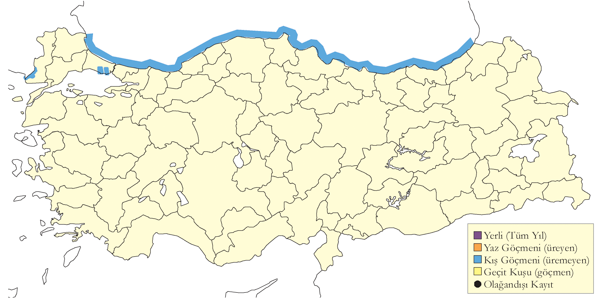
\includegraphics{images/harita_Page_026.png}

\textbf{Üreme}

Türkiye'de yuvalamaz. Avrasya ve Kuzey Amerika'nın kuzeyinde yuvalar.

\textbf{Alttürler ve Sınıflandırma}

Türkiye'de nominat alttürü bulunur.

\section{Pufla}\label{pufla}

\emph{Somateria mollissima}, Common Eider

\textbf{\emph{Karadeniz kıyılarında nadiren az sayıda görülür.}}

İlk üç kayıt şu şekildedir: 20 Eylül 1983'te Çernek Gölü'nde (Kızılırmak
Deltası) bir erkek (Dijksen \& Kasparek 1985), 3 Ocak 1984'te Göksu
Deltası'nda ölü bir dişi (Kasparek 1990), 1 Şubat 1997'de Sakarya Nehri
deltasının batısında, Kefken açıklarında iyi tanımlanmış ilk kışında bir
erkek ve iki dişi (Welch \& Welch 1998a) bulunmuştur. Bundan sonra Riva,
Terkos Gölü kıyıları, İğneada, Kızılırmak Deltası, İzmit Körfezi ve
Sakarya Karasu'da 20'den fazla kayıtta 1-3 birey tespit edilmiştir.

Türkiye'de üremez, en yakın üreme kolonisi Ukrayna kıyılarındadır.
Güvenilir kayıtların tümü, 1975 yılında Ukrayna'nın Karadeniz kıyısında
bir üreme alanının keşfedilmesinden sonra olmuştur. Bu popülasyon
1990'ların ortasına kadar 1000 çifte ulaşmış ve günümüze kadar artmaya
devam etmektedir.

Şubat 1929'un ilk yarısında Tarabya ile Beykoz arasında (İstanbul
Boğazı) gözlenen bir erişkin erkek (Kumerloeve 1970a), tanım olmadığı
için burada kabul edilmemiştir.

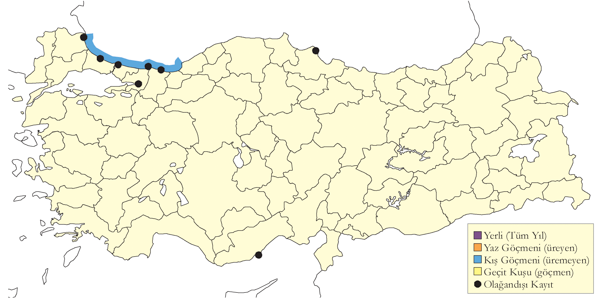
\includegraphics{images/harita_Page_027.png}

\textbf{Üreme}

Türkiye'de yuvalamaz. Ukrayna'daki koloni insan eliyle oluşturulmuş,
kolonideki kuşlar zamanlar doğallaşmıştır. Doğal yuvalama alanı Kuzey
Atlantik, Kuzey Buz Denizi ve Bering Boğazı'dır.

\textbf{Alttürler ve Sınıflandırma}

Ülkede gözlenen alttür nominat \emph{mollissima} (Kuzeybatı Avrupa)
alttürüdür.

\section{Kadife Ördek}\label{kadife-uxf6rdek}

\emph{Melanitta fusca}, Velvet Scoter

\textbf{\emph{Türkiye'de üreyen nüfus yok olmuştur. Karadeniz kıyılarına
az sayıda kışlar.}}

Doğu Anadolu'da az sayılarda kaydedilen çok lokal bir yaz konuğu idi. Az
sayıda yüksek irtifa göllerinde 3000 m'nin üstünde üremiş olduğu
düşünülür. Aktaş Gölü (Ardahan) kesin olarak ürediği tek alandır. 3 Ekim
1980'de 100 birey (Ven 1980) ve 14-15 Temmuz 1994'te aralarında
gençlerin de bulunduğu 725 birey (Yarar 1995) kaydedilmiştir.

Geçmişte Nemrut Dağı'ndaki (Tatvan) krater gölünde 20 çifte ürediği
düşünülmüştür. Ağrı Balık Gölü'nde geçmişte ürediği sanılmış, ancak
görünüşe göre Haziran 2001'de artık üremediğine karar kılınmıştır.
Çıldır Gölü'nde ürediği güçlü şekilde şüphelenilmiş, ancak teyit
edilmemiştir. Kars Aygır Gölü ve Muş Nazik Gölü'nde azami 32 birey yazı
geçirmiştir. Doğu Karadeniz kıyılarında kışlayan bireylerin yaz
aylarında da kaldığı gözlenmiştir.

Gürcistan'da yuvalamaya devam eden bireyler Karadeniz kıyılarına az
sayıda kışlar. Orta ve Doğu Karadeniz boyunca az sayıda kışlar. 1995
Aralık sonunda Yeşilırmak Deltası'nda 870 birey en yüksek kayıttır.
Nadir olarak Batı Karadeniz, Marmara'da ve güneyde Akdeniz kıyısında
kışlamıştır. Ocak 1970'de Burdur Gölü'nde 27 birey, Şubat 1966'da Mogan
Gölü'nde ve Ocak 2005'te Hazar Gölü'nde kaydedilmiştir. Son yıllarda
kaydedilen 50 birey.

4 Şubat 1917'de İstanbul Zeytinburnu açıklarında gözlenen iki birey ülke
için ilk kayıttır.

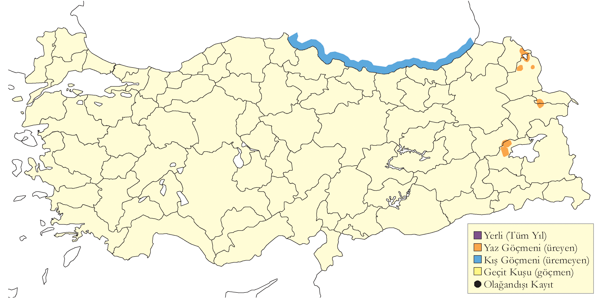
\includegraphics{images/harita_Page_028.png}

\textbf{Üreme}

\textbf{Yuvalama alanı:} Doğu Anadolu'daki iki ya da üç yüksek irtifa
gölünde üremiştir. Tüm çabalara rağmen Türkiye'de yuvası bulunamamıştır.
Şu anda Kafkasya popülasyonu sadece Gürcistan'da bir gölde
yuvalamaktadır.\\
\textbf{Yuvası:} Türkiye'de yuva bulunmamıştır ancak diğer yerlerde
yoğun bitki örtüsünün içine gizlenmiş şekilde yerde ve genellikle
göllerdeki adalarda yuva yapar.\\
\textbf{Yumurta sayısı:} Olağan yumurta sayısı 7-10'dur.\\
\textbf{Üreme dönemi:} Eski gözlemlere göre temmuz ve ağustos ayında
yuvalamıştır. \textbf{DOA}. 10 Temmuz 1967'de Nemrut Dağı'ndaki krater
gölünde iki, yedi ve dokuz hav tüylü küçük yavru ile birlikte üç dişi ve
20 Ağustos 1967'de Balık Gölü'nde dört, beş ve altı yavrulu üç dişi
kaydedilmiştir (Vielliard 1968). Küçük ördeklerin sadece yaklaşık bir
haftalık olduğu varsayılırsa yumurtlamanın haziranın ilk günlerinde
olduğu anlaşılmaktadır. 23 Ağustos 1972'de Nemrut Dağı'nda gözlenen
hemen hemen yarı gelişmiş yedi yavrulu bir dişi, yumurtlamanın haziranın
son haftasında olduğunu göstermektedir. 9 Temmuz 1985'te Nemrut Dağı'nda
beş çift ve iki genç birey gözlenmiştir. Son zamanlara ait bir üreme
kaydı yoktur ve 9 Haziran 2001'de Balık Gölü'ndeki adada yapılan
kapsamlı araştırmada ne yuva bulunmuş ne de erişkin görülmüştür.

\textbf{Alttürler ve Sınıflandırma}

Monotipik bir türdür. Eskiden Amerika ve Doğu Sibirya'da yaşayan Ak
Kanatlı Kadife Ördek \emph{Melanitta deglandi} ile aynı tür olarak kabul
ediliyordu.

\section{Kara Ördek}\label{kara-uxf6rdek}

\emph{Melanitta nigra,} Common Scoter

\textbf{\emph{Nadir kış konuğudur.}}

Karadeniz'de çoğunlukla eylül ve mart arasında çok az sayıda kaydedilen
kış göçmenidir. Düzenli olarak sadece Kızılırmak ve Yeşilırmak
deltalarının açıklarında 20 birey kışlamaktadır. Karadeniz kıyısında
toplam 20'den fazla kaydı vardır. Marmara ve Ege'de çok nadirdir,
Akdeniz'de sadece bir kere kaydedilmiştir.

9 Nisan 1967'de Kocaçay Deltası'nda kaydedilen bir birey ülke için kabul
edilebilir ilk kayıttır (OST 1969). Öncesinde Ege'de nadir bir kış
göçmeni olduğundan (Krüper 1875) ve İstanbul Boğazı ile Ceyhan
Deltası'ndaki şüpheli kayıtlardan (Kumerloeve 1961) bahsedilmiştir.

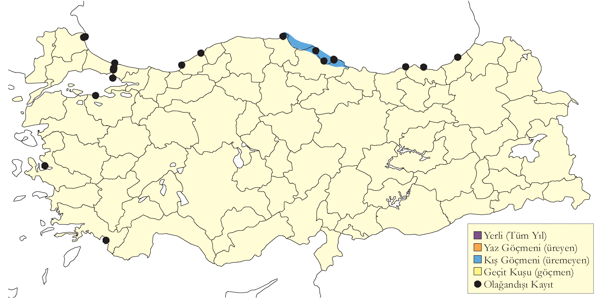
\includegraphics{images/harita_Page_029.png}

\textbf{Üreme}

Türkiye'de yuvalamaz. Avrasya'nın kuzeyinde yuvalar.

\textbf{Alttürler ve Sınıflandırma}

Monotipik bir türdür.

\section{Telkuyruk}\label{telkuyruk}

\emph{Clangula hyemalis}, Long-tailed Duck

\textbf{\emph{Nadir kış konuğudur.}}

Şubat 1893'te İstanbul (Büyük?) Çekmece'de, Alléon tarafından toplanan
genç bir dişi ülke için ilk kayıttır ve bu örnek Sofya Doğa Tarihi
Müzesi'nde görülebilir. Ardından, 13 Kasım 1968'de İzmit'te genç bir
birey kaydedilmiştir (OST 1975). Göksu Deltası Paradeniz Gölü'nde 1-2
Ocak 1986'da bir birey ve 5 Ocak 1989'da bir dişi (Kasparek 1990)
görülmüştür. Sakarya Nehri ağzında 18 Şubat 2004'te (Balmer \& Betton
2004b); 26 Şubat 2006'da Fırtına Nehri'nin ağzında birer birey
fotoğraflanmıştır. En güncel kayıtlara göre; 7-19 Ocak 2008'de
İğneada'da erişkin bir dişi, 13 Şubat 2008'de Kıyıköy'de bir erkek, 10
Aralık 2008'de İğneada'da bir birey (on üçüncü kaydı) ve 28 Mart 2009'da
Enez'de bir birey (on dördüncü kaydı) görülmüştür (Kirwan \& Özen 2014).

İstisnai olarak, Van Gölü'nden 1977 ile 1987 arasında mayıs ve haziran
aylarında yaz kayıtları mevcuttur. 10 Haziran 1977'de Gevaş'ın batısında
Horkum'da iki birey ve Tatvan ile Ahlat arasında üç birey (Beaman 1986),
22 Mayıs 1985'te Van'ın güneybatısında bir erkek (Martins 1989), 9
Haziran 1987'de Van Sazlığı'nda bir erkek ve 22 Haziran 1987'de Van'ın
10 km güneyinde bir birey (Kirwan \& Martins 1994) kaydedilmiştir.

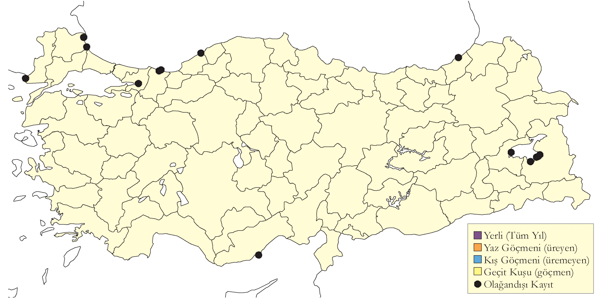
\includegraphics{images/harita_Page_030.png}

\textbf{Üreme}

Türkiye'de yuvalamaz. Kuzey İskandinavya dağlarında ve Rusya ve Kuzey
Amerika'nın tundra kuşağında yuvalar.

\textbf{Alttürler ve Sınıflandırma}

Monotipik bir türdür.

\section{Altıngöz}\label{altux131nguxf6z}

\emph{Bucephala clangula,} Common Goldeneye

\textbf{\emph{Nispeten yaygın ve az sayıda kış konuğudur.}}

Karadeniz, Marmara ve Ege'nin kıyı bölgelerinde ve daha nadir olarak iç
bölgelerdeki sulakalanlarda ekim sonu ve nisan sonu arasında nadir bir
kış konuğudur. En düzenli olarak Marmara ve Karadeniz bölgelerinde
görülür. Kışın ülke çapında görülen kuş sayısı nadiren 100 bireyi geçer.
3 Şubat 1992'de Kızılırmak Deltası'nın açıklarında gözlenen 200 birey,
kaydedilen en yüksek sayıdır. 2005-06 kışında Gediz Deltası'nda 72
birey, 3 Şubat 2002'de Gala Gölü'nde 60 birey sayılmıştır (Demirci
2002). Son yıllarda ilkbahar sonunda Doğu Karadeniz'de kaydedilmiştir.

1977 ile 1993 yılları arasında Doğu Anadolu'da, çoğunluğu Van Gölü'nde
olmak üzere, bir dizi yaz kaydı vardır ve bu kayıtlarda bazen birden
fazla birey gözlenmiştir. Bu kayıtlar, yakınlarda üreyen bir
popülasyonun ihtimalini düşündürmüştür (Kasparek 1992).

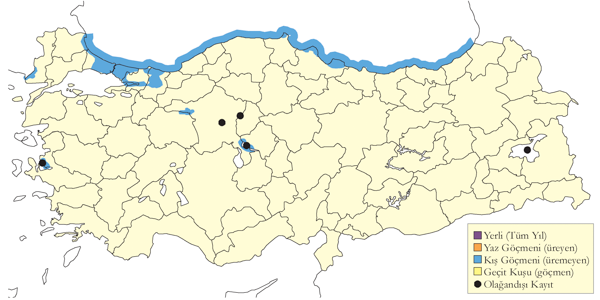
\includegraphics{images/harita_Page_031.png}

\textbf{Üreme}

Türkiye'de yuvalamaz. Avrasya ve Kuzey Amerika'nın kuzeyinde yuvalar.

\textbf{Alttürler ve Sınıflandırma}

Türkiye'de nominat alttürü bulunur.

\section{Sütlabi}\label{suxfctlabi}

\emph{Mergellus albellus,} Smew

\textbf{\emph{Kuzey bölgelerine az sayıda gelen bir kış konuğudur.}}

Kasımdan nisan ortasına kadar ülkenin batı ve orta bölgelerindeki
sulakalanlarda ve kıyılarda tipik olarak nadir ve muhtemelen düzensiz
bir kış konuğudur. En çok Marmara, Karadeniz ve İç Anadolu'da
kaydedilir. Her kış genellikle 100 bireyden daha azdır. Uluabat Gölü'nde
1967'de 300, 1969-70'de 1300, 1973'te 555, 1989'da 111 ve 1995'te 248
birey kaydedilmiştir. 1992'de Manyas Gölü'nde 102 ve 1993'te
Büyükçekmece'de 79 birey kışlamıştır.

Nisan 1987 sonunda Diyarbakır'da kaydedilmiştir. Doğu ve Güneydoğu
Anadolu'da oluşturulan büyük baraj göllerinde gözlenmesi beklenebilir.
Ocak 1979'da Irak Razzaza Gölü'nde gözlenen 1000'den fazla birey (Scott
\& Carp 1982), daha güneyde yüksek sayılarda kaydedilebileceğini
göstermektedir.

Ancak ne tuhaftır ki, türün ilk keşfi Strickland tarafından İzmir'den
alınan iki örnek ile yapılmıştır. Cambridge Üniversitesi Zooloji
Müzesi'ndeki koleksiyonda bulunan bu örnekler, 6 Ocak 1836'da alınan bir
erkek ve aynı yıl şubat ayında alınan bir dişiye aittir. 1946-48
yıllarında Çatalağzı açıklarında (Zonguldak) oldukça bol olduğu
gözlenmiştir (Ogilvie 1954).

11 Haziran 1969'da Eymir Gölü'nde (Ankara) bir erkek (OST 1972), 27
Haziran 1987'de Göründü'de (Van) bir dişi (Kirwan \& Martins 1994) ve 27
Mayıs 1995'te Uluabat Gölü'nde bir erkek ve iki dişi (Kirwan \& Martins
2000) olmak üzere yazın üç defa kaydedilmiştir.

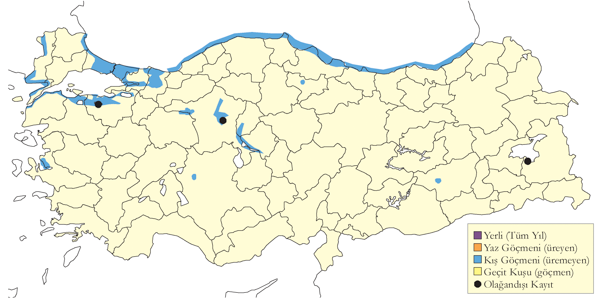
\includegraphics{images/harita_Page_032.png}

\textbf{Üreme}

Türkiye'de yuvalamaz. Avrasya'nın kuzeyinde yuvalar.

\textbf{Alttürler ve Sınıflandırma}

Monotipik bir türdür. Türkiye'de tanımlanmıştır.

\section{Büyük Tarakdiş}\label{buxfcyuxfck-tarakdiux15f}

\emph{Mergus merganser,} Common Merganser

\textbf{\emph{Nadir kış konuğudur.}}

Özellikle Marmara ve Karadeniz bölgelerinde az sayıda kaydedilen nadir
bir kış konuğudur. 1997-2007 arasında artan gözlemci aktivitesine karşın
sadece 10 kere kaydedilmiştir (Kirwan et al. 2003). Genellikle kıyısal
sulakalanlarda görülür ve en düzenli olarak Kızılırmak ve Yeşilırmak
deltalarında kaydedilir. Kızılırmak Deltası'nda görüldüğü en geç tarih
20 Mayıs'tır.

Doğu Anadolu'da şubat ve martta iki defa, yazın ise üç kere
gözlenmiştir; 11 Haziran 1970'de Pasinler ile Horasan arasında Aras
Nehri üzerinde bir çift, 7 Haziran 1986'da Van Gölü'nde bir birey ve 29
Haziran 1988'de Bendimahi Deltası'nda bir dişi ya da genç birey
kaydedilmiştir. Kurutulmadan önce Sevan Gölü (Ermenistan) havzasında
üreyen bir tür olduğu düşünülmüş, ancak ürediğine dair bir kanıt elde
edilmemiştir (Adamian \& Klem 1999).

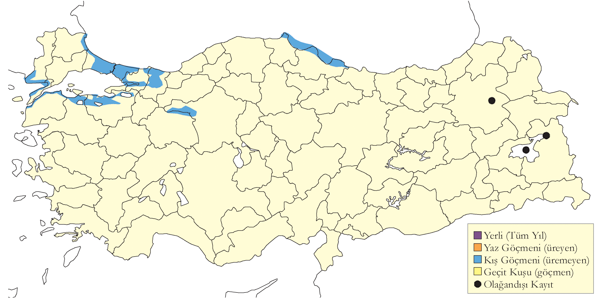
\includegraphics{images/harita_Page_033.png}

\textbf{Üreme}

Türkiye'de yuvalamaz. Avrasya ve Kuzey Amerika'nın kuzeyinde yuvalar.

\textbf{Alttürler ve Sınıflandırma}

Türkiye'de nominat alttürü bulunur.

\section{Tarakdiş}\label{tarakdiux15f}

\emph{Mergus serrator}, Red-breasted Merganser

\textbf{\emph{Nispeten lokal olarak ve orta sayılarda görülen bir kış
konuğudur.}}

Kıyısal alanlarda ekim sonu ve nisan sonu arasında kaydedilen kış
göçmenidir. En çok sayıda Doğu Karadeniz, Marmara ve Ege'de kaydedilir.
Gediz Deltası'nda düzenli olarak yaklaşık 100 birey konaklar; Şubat
1996'da 397 birey sayılmıştır. Büyük Menderes Deltası'nda Şubat 1993'te
67 birey ve Yumurtalık'ta 44 birey kaydedilmiştir. Ege ve Doğu
Akdeniz'deki alanlarda düzenli olarak önemli sayılarda kışlar (Eken
1997d). Akdeniz kıyılarında seyrek olsa da Kıbrıs'ta oldukça düzenli bir
türdür.

20-21 Mayıs 1994'te Göksu Deltası'nda geç kalmış bir birey
kaydedilmiştir (Birdquest Newsletter 23: 59). Tek yaz kaydı 11 Haziran
1964'te Amik Gölü'nde (Antakya) kaydedilen yedi veya sekiz bireydir
(Kumerloeve 1966-67).

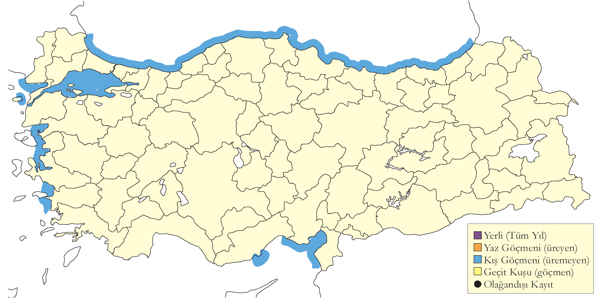
\includegraphics{images/harita_Page_034.png}

\textbf{Üreme}

Türkiye'de yuvalamaz. Avrasya ve Kuzey Amerika'nın kuzeyinde yuvalar.

\textbf{Alttürler ve Sınıflandırma}

Monotipik bir türdür.

\section{Dikkuyruk}\label{dikkuyruk}

\emph{Oxyura leucocephala,} White-headed Duck

\textbf{\emph{Lokal olarak az sayıda üreyen yaz konuğu, nispeten yaygın
ve yüksek sayıda bulunabilen geçit türü ve kış konuğudur.}}

İç Anadolu ve Doğu Anadolu'da tatlı veya acı (sodalı), sığ ve ötrofik
göllerdeki yoğun sazlık sulakalanlarda az ila orta sayıda yuvalar. Van
Gölü çevresinde ve Kars'taki küçük sulakalanlarda ürediği teyit
edilmiştir. Doğu Anadolu'daki diğer alanlardaki üreme durumu
belirsizdir. Niğde Akkaya Barajı'nda üremiştir (Kirwan 1994). Üreme
döneminde kaydedildiği Karadeniz Bölgesi'ndeki bazı alanlarda
yuvalayabilir. Doğu Akdeniz sulakalanlarında yaz kayıtları, üremeyen
bireylere aittir.

1980'lerin sonu ve 1990'ların başı arasında dört kilit alanda (Ereğli
Sazlığı, Hotamış Gölü, Sultansazlığı ve Kulu Gölü) üreyen İç Anadolu
popülasyonu muhtemelen 150 çiftin üzerindeydi (Robinson \& Can 1998).
Ancak 1990'ların ortasında Ereğli Sazlığı ve Hotamış Gölü'nün
kurumasıyla sayıları azalmış, Kulu Gölü'nde üremez olmuştur (Richardson
2003). Kozanlı Gökgöl ve Uyuz Gölü'nde az sayıda üremeye devam
etmektedir.

Mart ile mayıs başı arasında birçok alanda geçiş sırasında gözlenir. 23
Mart 1992'de Kızılırmak Deltası'nda 1246 birey ve Mart 1990'da Ereğli
Sazlığı'nda 508 birey toplanmıştır. Mayıs ve haziran arasında toplanan
sürüler muhtemelen üreme alanlarına dağılacak kuşlardan oluşur. Temmuz
ve eylül arasında toplanan sürüler ise üreme sonrası dağılmaya ve göç
almaya işaret eder. Temmuzda Kulu Gölü'nde 500 birey ve ağustosta Sodalı
Gölü'nde 600-1000 birey kaydedilmiştir.

Kışın Akdeniz'deki birkaç sulak alanda yüksek sayıda, İç Anadolu'da
genellikle daha az sayıda kaydedilir. Batı ve orta bölgelerindeki diğer
yerlerde ise daha nadiren, özellikle sert hava koşullarında kaydedilir.
Karadeniz Bölgesi'nde düzensiz olarak yüksek sayılarda kışlar. Bir dönem
dünya popülasyonunun \%50'sinden fazlasının Burdur Gölü'nde kışladığı
düşünülmüştür; buradaki sayımlarda 1987'de 6400, 1988'de 9230, 1989'da
6700 ve 1991'de 10.927 birey kaydedilmiştir (Green \& Anstey 1992).
Ancak 1992 sonrasında sayılarda azalma görülmüş; 1992'de 3264, 1993'de
3010 ve 1994'de 3337 birey sayılmıştır. Bu sayımlar son derece hassas
olup, eş zamanlı üç ekip tarafından ideal hava koşullarında
gerçekleştirilmiştir. Burdur Gölü'nde 1993'te 1991'e göre daha az genç
bireyin sayılması, daha düşük üreme başarısını gösterebilir. Bir
ihtimal, Kazakistan ve çevre ülkelerdeki üreyen nüfustaki azalış,
Türkiye'deki kışlama nüfusunun azalmasını açıklayabilir. Bu azalmada
şüphesiz kaçak avcılığın da payı vardır; 1992-93 kışında Burdur Gölü'nde
1000'den fazlasının vurulduğu tahmin edilmiştir. Ayrıca son yıllarda
Burdur Gölü'nün kuruma sürecinin başlaması ve tuzluluğun artması da bir
etken olabilir.

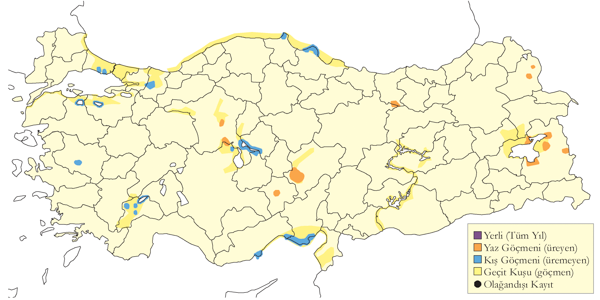
\includegraphics{images/harita_Page_035.png}

\textbf{Üreme}

\textbf{Yuvalama alanı:} Çoğunlukla büyük sulak alanların yakınlarında
genellikle 10 hektardan küçük ve 2 metreden sığ, sualtı vejetasyonu bol
ve su aynalarının bulunduğu geniş sazlıklara sahip tatlı su göllerinde
ya da sodalı göllerde ürer (Anstey 1989). Aynı alanda birkaç çift
üreyebilir.\\
\textbf{Yuvası:} Yuva, ölü saz gövdeleri ile diğer sucul bitkilerin
düzgün bir kâse oluşturacak şekilde örülmesi ile oluşturulmuş, birkaç
tutam açık gri tüy ile astarlanmış dayanıklı bir yapıdır.\\
\textbf{Yumurta sayısı:} Bir yuvada en fazla 10 yumurta kaydedilmiştir.
19 Haziran 2004'te aynı gölde diz boyu derinliğindeki suda yoğun bir
sazlığın içinde iyice gizlenmiş bir şekilde suyun üzerinde dikey
sazların dibine tutturularak yapılmış bir yuvada on yumurtalı
tamamlanmış bir kuluçka bulunmuştur. Diğer yerlerde olağan yumurta
sayısı 5-12'dir. Dikkuyruk, vücut ölçülerine göre son derece büyük ve
ağır yumurtalar koyar; yuva bu ağırlık nedeniyle suya batabilir.\\
\textbf{Üreme dönemi:} Mayıs başı ve temmuz başı arasında yumurta koyar.
Eylül sonuna kadar yavrular görülebilir. \textbf{İÇA.} 13 Temmuz 1987'de
Kulu Gölü'ndeki sazlıkların içindeki yuvada yedi yumurta gözlenmiştir;
muhtemelen dişinin kuluçkaya ara vermesi nedeniyle yuva ve yumurtalar
kısmen su altında kalmıştır (Anstey 1989). Üreme kayıtlarının çoğu 3-10
yavrudan oluşan gruplardır: İç Anadolu'daki en erken kayıt, 5 Haziran
1975'te Kulu Gölü'nde gözlenen üç büyük ve üç hav tüylü yavrudur; bu
durum yumurtlamanın mayıs başında olduğunu gösterir. 6 Ağustos 1972'de
(kurutulmuş) Gönenç Gölü'nde 20 günlük beşer yavrularıyla iki dişi ve
dört günlük altı yavrulu bir dişi gözlenmiştir; bu kayıtlar
yumurtlamanın haziran ortası ile temmuz başında olduğunu göstermektedir.
İç Anadolu'da, temmuz ve ağustosta birçok yavrulu aile kaydedilmiştir.
\textbf{DOA.} Haziran-eylül ayları arasında Van Gölü'nde 9 Haziran 1987
ve 14 Haziran 1990'da gözlenen genç bireyler, yumurtlamanın mayıs
ortasında olduğunu göstermektedir. Temmuz-ağustos arasındaki diğer
kayıtlar, yumurtlamanın haziran ortasında başladığını düşündürmektedir.
Erçek Gölü yakınlarındaki küçük bir gölün ortasında dikey sazlardan
oluşan bir adada bir yuva bulunmuştur; sucul bitkiler kullanılarak
sazların dibine yapılmış olan yuvada 11 Haziran 2001'de iki yumurta
olduğu, kuluçkanın henüz tamamlanmadığı gözlenmiştir; alanda sekiz erkek
ve yedi dişi birey kaydedilmiştir. Ancak oldukça kapsamlı bir araştırma
yapılmasına rağmen başka bir yuva bulunmaması, üremenin henüz tam
anlamıyla başlamadığını göstermektedir.

\textbf{Alttürler ve Sınıflandırma}

Monotipik bir türdür.

\bookmarksetup{startatroot}

\chapter{Tavukgiller}\label{tavukgiller}

\section{Orman Horozu}\label{orman-horozu}

\emph{Lyrurus tetrix}, Black Grouse

\textbf{\emph{Türkiye'de soyu tükenmiştir. Eskiden lokal olarak az
sayıda bulunan yerli türdü.}}

Relikt bir popülasyon, 19. yüzyılın sonuna kadar İstanbul çevresinde
devam etmiştir (Kasparek 1990), ancak anlaşıldığı kadarıyla avlanma
sonucunda soyu tükenmiştir. Türkiye'de yaşadığı ilk iki bilim insanı
tarafından tespit edilmiştir (Rigler 1852, Tchihatchef 1864). Son olarak
İstanbul Alemdağ çevresinde bulunduğu düşünülmüş (Reiser 1904) ve
şehirde satılan, nereden geldiği bilinmeyen ölü erkek bireyler tespit
edilmiştir (Mathey-Dupraz 1920--24). Aynı dönemde Bulgaristan
popülasyonunun da ciddi oranda azaldığı kaydedilmiştir (Elwes \& Buckley
1870); bu durum muhtemelen avcılığa bağlanmaktadır. Tür burada da uzun
süreden beri tükenmiş durumdadır. Genel olarak türün küresel yayılış
alanı kuzey ve batıya doğru daralmıştır (Hagemeijer \& Blair 1997,
Handrinos \& Akriotis 1997, Madge \& McGowan 2002). Yunanistan'da 1935
yılından bu yana Selanik ve Rodop Dağları çevresinden dört kayıt
bulunmaktadır.

\textbf{Üreme}

Türkiye'de yuvalamaz. Kuzey Avrasya'daki orman kuşağında yuvalayan yerli
bir türdür.

\textbf{Alttürler ve Sınıflandırma}

Türkiye'de yaşamış popülasyon muhtemelen nominat \emph{tetrix} alttürüne
aittir. Literatürde \emph{Tetrao} cinsi altında da sınıflandırılmıştır.

\section{Dağ Horozu}\label{daux11f-horozu}

\emph{Lyrurus mlokosiewiczi}, Caucasian Grouse

\textbf{\emph{Lokal olarak az sayıda bulunan yerli bir türdür.}}

Doğu Karadeniz Dağları'nın kuzey yamaçlarında bulunur. Ağaç sınırının
üstündeki 1800-3000 metre arasındaki ormangülü (\emph{Rhododendron})
örtüsünde yaşar. 3000 metre üzerinden gelen üreme kayıtları (Başkaya
2003) doğrulama gerektirir; ancak, neredeyse yerleşim yerlerine yakın
(muhtemelen 15 kilometreye kadar) ve sonbahar ile kış mevsimlerinde
düşük yüksekliklerde, ağaç sınırının altında ve muhtemelen özellikle
şiddetli soğuklarda daha da düşük yüksekliklerde bulunurlar. Yayılış,
bodur ormangülü \emph{Rhododendron} ile alpin çayır kuşağının altındaki
huş (\emph{Betula}) içeren yamaçlar üzerine yoğunlaşmıştır (Atkinson et
al. 1995).

Artvin'in güneydoğusundan Gürcistan sınırı üzerinde Posof'a kadar
Yalnızçam Dağları'nda dar bir alanda bulunurlar. Yerel halktan alınan
bilgiler ışığında Gümüşhane'nin batısında, Giresun çevresinde ve
muhtemelen Bingöl'e kadar güneyde, Cilo Dağları'nda bulunması olasıdır.

Türün lokal olarak nadir ya da Doğu Karadeniz kıyı şeridi boyunca yaygın
yerli olduğu gösterilene kadar, geçtiğimiz yıllar içerisindeki
kayıtlarda görülen aşırı düzeydeki yetersizlik ile özellikle 1980 öncesi
kayıtlardaki eksiklik, türün Türkiye'de çok az bilinmesine neden
olmuştur. G. Neuhäuser, Eylül 1943 tarihinde yüksek olasılıkla Türkiye
için ilk kayıt olan bir çift huş tavuğunu Rize ve Erzurum arasındaki
dağlardan toplamıştır (Kumerloeve 1961).

Türkiye popülasyonunun muhtemelen \%90'ının görüldüğü Kaçkar
Dağları'nda, özellikle Sivrikaya çevresinde, 1993 yılında
gerçekleştirilen gözlem çalışmalarında kur yapma amacıyla bir araya
toplanan (lek poligini) 134 erkek gözlenmiştir. O tarihlerde yapılan
tümevarımla toplam popülasyonun 2000 bireyden fazla olduğu tahmin
edilmiştir (Magnin \& Yarar 1997). Türkiye popülasyon büyüklüğü, son
zamanlardaki çalışmalara göre 1508-2675 birey arasında ölçülmüş ve tür
45 coğrafi yerde kaydedilmiştir (Isfendiyaroğlu et al. 2007). Bu coğrafi
yerlerin 29 tanesi yakın bir zaman dilimi içerisinde keşfedilmiştir.
Bunlardan 4 tanesi nispeten ayrık popülasyonlardır. Türün yayılış
sınırlarını ve popülasyon büyüklüğünü tam olarak belirlemek için
bilgisayar modellemesi kullanılmıştır (Gottschalk et al. 2007). Ancak,
modellemenin sonuçları bilinen ve yayılış haritasında gösterilen alanı
genişletilememiştir. Bununla birlikte 4900 bireylik popülasyon tahmini,
önceki en iyimser tahminlerden bile çok yüksek olmuştur.

Türkiye popülasyonu, yaylaların tatil konutlarına dönüşmesi sonucunda
artan yol inşaatları nedeniyle yaşam alanlarının terkedilmesinden
etkilenmekte ve nesli tehlike altına girmektedir. Daha az ölçüde avlanma
baskısından (özellikle sonbahar döneminde görülen bir problem) ve tür
için bir tehdit kaynağı olarak listelenen aşırı otlatma bugün kaydedilir
ölçekte değildir; ancak, bu durumun izlenmesi gereklidir. Türün
popülasyonlarının dengede ya da azalmakta olup olmadığını ortaya koymak
için türün popülasyonu ve yayılışı ile ilgili tarihsel bilgiler yetersiz
düzeydedir; ancak, popülasyonların azalmasından şüphelenilmektedir.

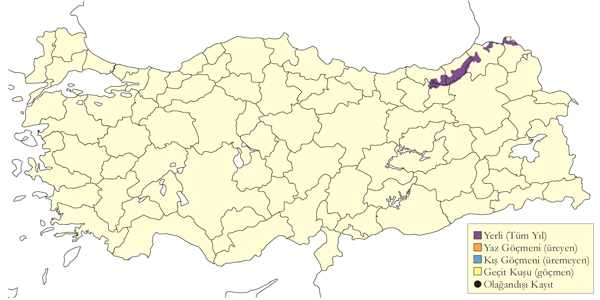
\includegraphics{images/harita_Page_037.png}

\textbf{Üreme}

\textbf{Yuvalama alanı:} Türkiye'de sadece iki yuvanın en iyi bilindiği
lokalite, Sivrikaya'da (Rize) bulunmuştur. İlk yuva 2800-3000 metrede,
bodur \emph{Rhododendron} çalılarının bulunduğu 3 hektarlık bir alanda
yer almıştır.\\
\textbf{Yuvası:} Yuva, yoğun, kısa (1 metre) ve çok dallı çallılarda
iyice gizlenmiş olup, kökten çıkan dalların arasında, zeminde sığ bir
çanak şeklinde yapılmış, kuru dallar ve birkaç kuru \emph{Rhododendron}
yaprağıyla astarlanmıştır.\\
\textbf{Yumurta sayısı:} Bu yuvada 6 Temmuz 1991 tarihinde 5 yumurta
kaydedilmiştir (Temple-Lang \& Cocker 1991).\\
\textbf{Üreme dönemi:} Erkekler, özellikle şafak ve gün batımında,
eşeylerin çiftleşme amaçlı karşılaştığı alanlarda bir araya gelerek kur
gösterileri (nümayiş) yaparlar. Diğer kayıtlarda dişinin uçarak
uzaklaştığı bir yuvada 12 Temmuz 1993 tarihinde 4 yumurta görülmüş ve
bir yumurta kabuğu 11 Haziran 1997 tarihinde bulunmuştur. Bir erişkin
dişi ile tam gelişmemiş iki genç, 12 Haziran 2003 tarihinde Ardahan,
Posof'da gözlenmiş ve yumurtlama zamanının mayıs başında başladığını
göstermiştir. Başka yerlerde, yaygın kuluçka küme büyüklüğü 5-6 (2-10)
adettir. Ermenistan'da, 30 Mayıs 1984'de bulunan bir yuva 8 yumurta
içermiş ve bu yuvada ilk yumurtanın 21-23 Mayıs 1984 tarihinde
bırakıldığı belirlenmiştir. Bir diğer yuva 20 Mayıs 1985 tarihinde
yumurta içermekte olup, ilk yumurta 13-16 Mayıs 1985 tarihinde
bırakılmıştır. Bir dişi üç genç bireyle (ergin büyüklüğünün \%25'ine
ulaşmış) birlikte 5 Haziran 1980 tarihinde ve bir diğeri 26 Temmuz 1980
tarihinde tamamiyle büyümüş 5 genç içermektedir (Adamian ve Klem 1999).
Ermenistan'dan üreme döneminin daha erken gösteren kayıtlar, Türkiye
kayıtlarının normal üreme dönemini yansıtıp yansıtmadığı hakkında bazı
şüpheleri ortaya koymuştur.

\textbf{Alttürler ve Sınıflandırma}

Monotipik bir türdür. Rusca literatürde çoğunlukla \emph{Lyrurus} cinsi
altında, Batı Avrupa'da \emph{Tetrao} altında sınıflandırılmıştır.
Farklı uygulamaların özeti için bkz. (Gokhelashvili et al. 2003).

\section{Çilkeklik}\label{uxe7ilkeklik}

\emph{Perdix perdix}, Grey Partridge

\textbf{\emph{Lokal olarak az sayıda bulunan bir yerli türdür.}}

Özellikle ovalardaki tarım alanlarında, uzun boylu ot topluluklarının
kenarlarında ve 2250 metreye kadar birincil yarı step alanlarda ürer.
Özellikle İç Anadolu ve Doğu Anadolu'nun kuzey kısımlarında ve Karadeniz
Bölgesi'nin iç kısımlarında yuvalar. Güney Anadolu'daki yayılış alanının
çoğunda ise çok nadir ve lokaldir.

Geçtiğimiz 20 yıl içerisinde tarımın yoğunlaşması, aşırı otlatma ve
avlanma nedeniyle popülasyonu önemli derecede azalmıştır. Trakya'da
yabani nesli tükenmiş olup, çeşitli kurum ve kuruluşlar tarafından
nüfusu takviye amaçlı genetik yapısı farklı olan yetiştirilmiş kuşlar
salınmış, ancak bu kuşlar yeni bir nüfus oluşturamamıştır. Belki de
Bulgaristan'daki yabani kuşların Türkiye'ye kendiliğinden gelmesi
beklenmelidir.

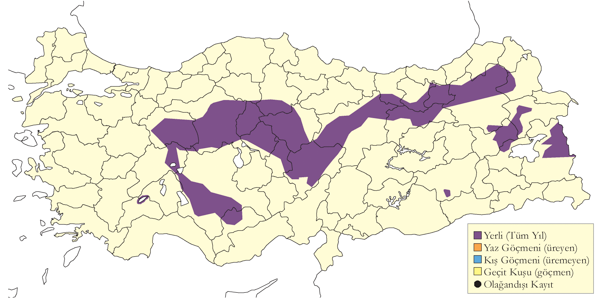
\includegraphics{images/harita_Page_042.png}

\textbf{Üreme}

\textbf{Yuvalama alanı:} Genellikle açık tarım alanlarında ürer.\\
\textbf{Yuvası:} Türkiye'deki bir yuvası betimlenmemiştir, ancak diğer
yerlerden gelen bilgilere göre yuva, ot ve ölü yapraklarla astarlanmış,
genellikle vejetasyon içerisine iyi bir şekilde gizlenmiş ve zeminde yer
alan sığ oyuklar şeklindedir.\\
\textbf{Yumurta sayısı:} 19 yumurta koyabilir. Diğer yerlerdeki yaygın
kuluçka küme büyüklüğü 9-20 (23) arasındadır. Bazen iki dişinin aynı
kuluçkayı paylaşması nedeniyle büyük kuluçkalar da kaydedilebilir.\\
\textbf{Üreme dönemi:} Mayıs ayında yumurtlamaya başlar. Yavrular:
\textbf{İÇA.} 11 Haziran 1977 tarihinde bir genç ile bir ergin Mogan
Gölü'nde, 16 Temmuz 1977 tarihinde 8 genç Emir Gölü'nde ve 28 Ağustos
1984 tarihinde 7 bireylik bir aile Çavuşcu Gölü'nde kaydedilmiştir.
\textbf{GDA.} Diyarbakır yakınlarında, 16 Mayıs 1999 tarihinde gevenle
(\emph{Astragalus sp.}) örtülü bir yamaçta on yumurta içeren bir yuva 27
Mayıs'ta 19 yumurta içermiştir (Karakaş \& Kılıç 2002).

\textbf{Alttürler ve Sınıflandırma}

Trakya'da nominat \emph{perdix} alttürü, Anadolu'da ise \emph{canescens}
alttürü bulunmaktadır. Doğaya salınan farklı orijinden bireylerin yerel
kuşlarla karışması nedeniyle türün yayılış alanı içindeki coğrafi
varyasyonu oldukça karışıktır (Madge \& McGowan 2002).

\section{Sülün}\label{suxfcluxfcn}

\emph{Phasianus colchicus}, Common Pheasant

\textbf{\emph{Lokal olarak az sayıda bulunan yerli türdür.}}

Türkiye'deki yerli popülasyonun yayılış alanı büyük ihtimalle Batı ve
Orta Karadeniz kıyısındaki kıyısal ormanlar, ``psödomaki'' olarak
bilinen Akdeniz bitki örtüsü ve fundalıklarla sınırlıydı. Tüm bilinen
tarihi ve güncel lokaliteler haritalanmıştır (Kasparek 1988b), bu
yayılış noktalarının çoğu Güney Marmara ve Orta Karadeniz'de yoğunlaşmış
olup, en batıda Trabzon'a kadar doğuya ulaşır. Türkiye'deki yerli bir
popülasyonun varlığı bir dönem şüpheyle karşılanmışsa da (Madge \&
McGowan 2002), İstanbul bölgesinden 1792'den sonra gelen kayıtlar yerli
popülasyonun varlığını desteklemiştir (Kasparek 1988b).

Doğal nüfusu neredeyse tamamen kaybolmuştur; yabani kuşların çoğunun
soyu av için salınan kuşlara dayanır. Toplam stoktaki yerli kuşların
varlığı çok sınırlıdır ve saf yerli kan, devamlı olarak av için salınan
yabancı ve karışık kuşların içinde eriyip gitmiştir. Bugün doğal
popülasyondan geriye kalanların Sinop bölgesinde ve yakın zamana kadar
Kızılırmak Deltası ve çevresinde bulunması olasıdır. İç Anadolu, Ege ve
Akdeniz'de görülen sülünler, şüphesiz doğaya salınan kuşlardan
türemiştir.

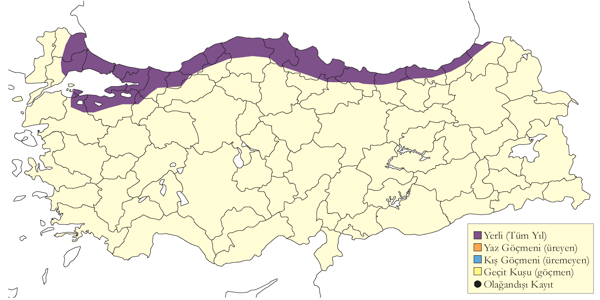
\includegraphics{images/harita_Page_044.png}

\textbf{Üreme}

\textbf{Yuvalama alanı:} Kıyısal ormanlar, ``psödomaki'' olarak bilinen
Karadeniz bitki örtüsü ve fundalıklar.\\
\textbf{Yuvası:} Bu konuda Türkiye'den bir bilgi yoktur. Zemine
yuvalar.\\
\textbf{Yumurta sayısı:} Diğer yerlerde 6-11 yumurta koyar.\\
\textbf{Üreme dönemi:} Diğer yerlerde mayıs ve haziran arasında yumurta
koyar.

\textbf{Alttürler ve Sınıflandırma}

Yerli popülasyon, nominat \emph{colchicus} alttürü altında
sınıflandırılmıştır (Dement'ev \& Gladkov 1967, Roselaar 1995). Hatalı
olarak Kuzey Kafkasya'da bulunan \emph{septentrionalis} alttürüne dahil
edilmiştir (Kumerloeve 1961).

\section{Turaç}\label{turauxe7}

\emph{Francolinus francolinus}, Black Francolin

\textbf{\emph{Güneydoğu Anadolu ve Doğu Akdeniz'de yaygın olarak çok
sayıda bulunan yerli türdür.}}

Çukurova ve Göksu Deltaları çevresinde, ayrıca Suriye sınırında Fırat ve
Dicle nehirleri boyunca ürer. Doğu Akdeniz popülasyonu en iyi
izlenendir. Çukurova popülasyonunun 75 çiftinin Akyatan Gölü çevresinde
yoğunlaştığı, toplamda 85 çifte ulaştığı kaydedilmiştir (Magnin \& Yarar
1997). Göksu Deltası'nda, çoğu kumullarda olmak üzere 50 üreme çifti
kaydedilmiştir (Magnin \& Yarar 1997). En yaygın bulunduğu bölge olan
Güneydoğu Anadolu'da yaklaşık 15 lokaliteden kaydı vardır (Welch 2004).

Doğu Akdeniz'deki popülasyonu dikkate alınarak mevcut durumu ve
ekolojisi derlenmiştir (Berk 1988). Doğu Akdeniz'deki bazı yerlerde tür
için koruma tedbirleri uygulanmıştır. Güneydoğu Anadolu'da ise tarımsal
faaliyetlerin artması sonucu hem sayılarının arttığı hem de yayılış
alanının genişlediği düşünülmektedir.

Eskiden Güneydoğu Marmara ile Ege Bölgesi'nin güney kıyılarının bazı
bölümlerinde yerli olarak kaydedilmiştir (Kumerloeve 1963b). Ancak, her
iki bölgede 19. yüzyıl içinde ortadan kalkmıştır. İstanbul Boğazı
çevresinden 1850'li yıllardan gelen tek bir kayıt vardır. Göller Bölgesi
ile Anti-Toroslara kadar kuzeyde, 600 metreye kadar oldukça lokal olarak
kaydedilmiştir (Kumerloeve 1961). Ekim 2003 tarihinde Tavas, Denizli
çevresinden muhtemelen tutsak bir bireyin kaçması sonucu güncel bir
kayıt gelmiştir. 1960'lı yıllarda Köyceğiz Gölü'ndeki kayıtlar, Batı
Akdeniz'deki son kayıtlardır. 1990'lı yıllara kadar Akdeniz bölgesindeki
yayılışı İçel, Adana, Osmaniye ile sınırlıydı. Sayıları artan kuşların
yavaş yavaş Batı Akdeniz'e doğru ilerlediği kaydedilmiştir. Örneğin
Antalya Havaalanı arazisinde 2010'dan beri kaydedilmektedir.

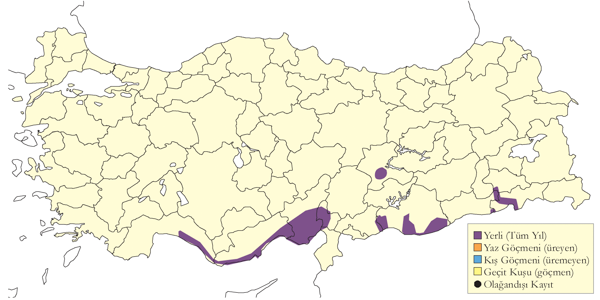
\includegraphics{images/harita_Page_041.png}

\textbf{Üreme}

\textbf{Yuvalama alanı:} Çalı ve çalı dışındaki bitki örtüsüne sahip
kumullar ile ot, çalı ve bodur bitkilerin arasındaki oyuklarda yaşarlar.
Ayrıca, olgunlaşmamış çalıların bulunduğu nemli (ıslak olmayan) alanlar,
nehir kıyıları ve sık ılgın (\emph{Tamarix}) çalılarından oluşmuş sık
topak şeklindeki çalılık alanlarda ve mısır tarlalarında ürerler. Kum
tepelerinde (her 2-5 hektarda bir erkek) ve tarım alanlarında (15-30
hektarda bir erkek) yüksek yoğunluktadırlar (Berk 1988).\\
\textbf{Yuvası:} Göksu Deltası'ndaki kum tepelerinde 17 Haziran 1992
tarihinde bulunan eski yuva, astarlanmamış, kum içerisinde birkaç bitki
parçasıyla çevrelenmiş sığ bir oyuk şeklindedir ve zemininde bir tutam
ot içermektedir.\\
\textbf{Yumurta sayısı:} Türkiye dışında yumurta sayısının genellikle
8-12 arasında olduğu bilinir.\\
\textbf{Üreme dönemi:} Mart sonu ve nisan arasında yumurta bırakır.
Yavrular mayıs ortasında dolaşmaya başlar ve temmuz ortasına kadar
görülebilir. Manchester Müzesi'ndeki üç yumurta (tamamlanmamış bir
kuluçkadan) İzmir yakılarından 10 Mayıs 1899 tarihinde alınmıştır. Tring
Doğa Tarihi Müzesi'ndeki dört yumurtanın ikisi Mersin'den 7 Mayıs 1884
tarihinde ve diğer ikisi 15 Mayıs 1899 tarihinde Anadolu'da bilinmeyen
bir lokaliteden alınmıştır. \textbf{AKD.} Göksu Deltası'ndaki kum
tepelerinde, 17 Haziran 1992 tarihinde muhtemelen bir önceki yıldan
kalmış bir yuva kaydedilmiştir. Yuvada güneşten etkilenmiş ve solgun
renklere sahip yumurta kabukları bulunmuştur. Yuva, astarlanmamış, kum
içerisinde birkaç bitki parçasıyla çevrelenmiş sığ bir oyuk şeklindedir
ve zemininde bir tutam ot içermektedir. Göksu'da, en azından 1-2 günlük
7 genç ile bir dişi 5 Mayıs 2004 tarihinde kaydedilmiştir. Bu kayıt, ilk
yumurtanın 9 Nisan'da bırakıldığını göstermektedir. Bir ergin ile bir
genç kuş 20 Temmuz 1986 tarihinde gözlenmiştir. Çukurova'da, yerel halk
yavruları 10 Mayıs 1986 tarihinde yakalamıştır (yaygın oldukları
bildirilmiştir). Bu tarih, yumurta bırakma zamanının yaklaşık nisan
ortasında olduğunu göstermektedir. Ötüşteki artış ise nisan ayının
ikinci yarısı ile mayıs ayının ilk yarısında tepe yapmaktadır (Berk
1988). Eski avcıların kayıtlarına göre ``dişi kuşlar mart sonu ile nisan
ayı içerisinde yuvaları ve yumurtaları ile meşguldürler'' (Banoğlu \&
Burr 1953). Yumurtalar, keklik (kınalı keklik) yumurtaları büyüklüğünde
ve açık yeşil renktedir; Seyhan ve Ceyhan kıyılarındaki sık örtüşe sahip
bodur ağaçlıklar arasında zemine bırakılır. Dörtyol ve Alik civarında,
dik ve derin vadilerdeki kayalıkların sınırlarına ya da adalar
arasındaki saz yatakları araları ile bodur ağaçlıklar ve çalı topakları
içine yuvalanırlar. Eskiden Adana civarındaki düzlüklerde çok sayıda
görülürlermiş. \textbf{GDA.} Birecik'in güneyindeki geniş mısır
tarlalarında erginlerin sesleri duyulmuş, üredikleri kesin olarak
kaydedilmiştir.

\textbf{Alttürler ve Sınıflandırma}

Türkiye'de nominat alttürü bulunur. Meinertzhagen tarafından Amik Gölü
bölgesinden tanımlanmış \emph{billypayni} alttürü sinonim olarak kabul
edilmektedir.

\section{Urkeklik}\label{urkeklik}

\emph{Tetraogallus caspius}, Caspian Snowcock

\textbf{\emph{Yüksek dağlarda lokal olarak az sayıda bulunan yerli
türdür.}}

Yüksek dağların yerlisidir. Üç önemli popülasyon Doğu Karadeniz Bölgesi,
Yüksekova ile Hakkari'ye ve İran sınırına kadar uzanan Doğu Anadolu'nun
dağlık kısımları ve en batı sınırını oluşturan Toroslar olarak
belirtilebilir. En batıda Toros silsilesinde Bolkar ve Melendiz
dağlarında kaydedilmiştir. Yaz aylarında genellikle 2400 metrenin
üzerinde kaydedilir. Ancak yazın Mersin'in kuzeyindeki dağlarda 2000
metrenin altında da görülmüştür. Ara sıra sonbahar döneminde 60 bireye
kadar büyük gruplar oluştururlar; bu grupların bazıları kış ortasında
alçak bölgelere inenler olabilir.

Eski kayıtlarda, en batıda Geyik Dağı, Alanya'nın kuzeyi ve Antalya'nın
dağlık alanlarında gözlenmiştir (Kumerloeve 1961). Daha batıda Akdağlar
ve Beydağları'ndaki sürekli kar örtüsüne sahip zirveler de uygun
yüksekliğe sahip alanlardır.

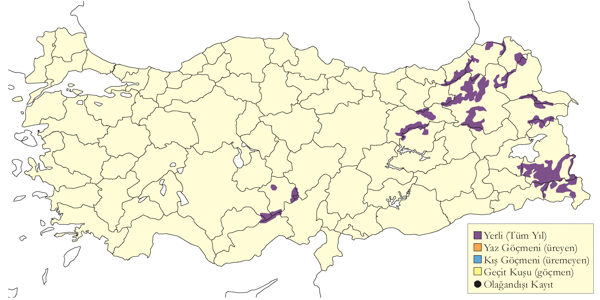
\includegraphics{images/harita_Page_038.png}

\textbf{Üreme}

\textbf{Yuvalama alanı:} Özellikle 2400 metre üzerinde, alpine
çayırlarla kaplı, dik kayalıkların ve yarların olduğu, yıl boyunca karlı
bölgelerde ürerler.\\
\textbf{Yuvası:} Karanfil Dağı'nda 2100 metre yükseklikte 23 Nisan 1876
tarihinde, bir dişi çıkıntılı bir kaya ve ardıç kökü ile sarılmış bir
yuvanın bulunduğu dik bir su yolundaki küçük bir kaya üzerinden
uçmuştur. Yuva, taşlı toprak üzerinde derin yuvarlak bir oyuk olup
yetersiz düzeyde kuru otlar ve birkaç kuş tüyüyle astarlıdır. Bu yuvada
altı yumurta kaydedilmiştir. 25 Nisan 1876 tarihinde Bolkar
Dağları'ndaki iki yuva benzer özelliklerde kaydedilmiştir. Ancak bir
tanesi yeşil köknar ibreleri ile astarlanmıştır.\\
\textbf{Yumurta sayısı:} Yukarıdaki üç yuvada altı ve dört yumurta
kaydedilmiştir. İki yumurta Manchester Müzesi'nde, diğerleri ise Tring
Doğa Tarihi Müzesi'nde saklanmaktadır.\\
\textbf{Üreme dönemi:} \textbf{KAR.} Sivrikaya'da (Rize) beş genç ile
bir ergin 12 Haziran 1989 tarihinde küçük karlı alanları geçerken
kaydedilmiştir. \textbf{AKD.} Nisan 1876 tarihinde Toroslar Aladağlar
bölgesindeki yuvaları araştırmıştır (Danford 1877-78) . 8 Temmuz 1986
tarihinde Aladağlar'da 1-2 haftalık 5 genç ile bir ergin gözlenmiştir.
İlk yumurta 21 Mayıs tarihinde bırakılmış olmalıdır. Çil Keklik
büyüklüğünde 5-6 ferik ile bir dişi 3-5 Ağustos 1967 tarihinde
kaydedilmiştir (Vielliard 1968). 19 Ağustos 2000 tarihinde, bazıları
erginlerden belirgin derecede küçük 3-4 ferikli en azından üç aile grubu
kaydedilmiştir.

Ermenistan'da ortalama yumurtlama dönemi 10-15 Mayıs, kuluçka dönemi ise
20-30 Mayıs arasındadır. Yavrular 13 Haziran tarihinde kaydedilmiştir
(Adamian \& Klem 1999). Gençlere ait bazı erken kayıtlar ilk yumurtanın
23 Nisan veya öncesinde bırakıldığını ortaya koymaktadır. Nisan sonu ile
mayıs başını içeren iki kayıt Danford'un Türkiye'de kaydettiği yuva
tarihleri ile kabaca uyum göstermektedir.

\textbf{Alttürler ve Sınıflandırma}

Monotipik bir türdür. Eskiden Hakkari ve Zagros Dağları'ndaki kuşların
\emph{semenowtianschanskii} (Zarudny, 1908), Toros Dağları'ndaki
kuşların \emph{tauricus} (Dresser, 1876) ve Erzurum bölgesindeki
kuşların \emph{challayei} isimli ayrı alttürler olduğu düşünülmüştür.

\section{Kum Kekliği}\label{kum-kekliux11fi}

\emph{Ammoperdix griseogularis}, See-see Partridge

\textbf{\emph{Güneydoğu Anadolu'da yaygın olarak çok sayıda bulunan
yerli türdür.}}

İlk zamanlarda çoğunlukla Suriye sınırına 50 km mesafedeki 15
lokaliteden bilinirdi. Ancak, Güneydoğu Anadolu'da yürütülen kapsamlı
bir biyoçeşitlilik araştırması, uygun habitatların bulunduğu alanlarla
birlikte türün hemen hemen 50 coğrafi yerde bulunduğunu göstermiştir
(Zeydanlı et al. 2005). Çoğunlukla az sayıda gözlenir, ancak sonbaharda
40 bireylik gruplar kaydedilmiştir.

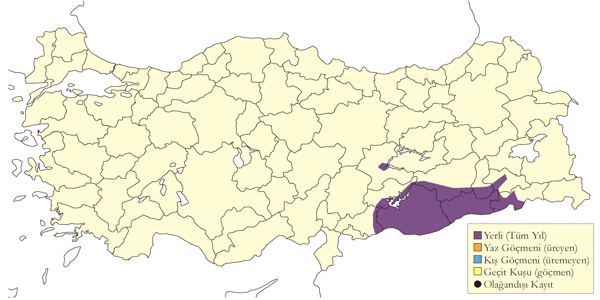
\includegraphics{images/harita_Page_040.png}

\textbf{Üreme}

\textbf{Yuvalama alanı:} Güneydoğu Anadolu'da zayıf vejetasyon örtüsüne
sahip kurak kayalık alanlarda üremektedir.\\
\textbf{Yuvası:} Türkiye içerisinde yuva ve yumurta tanımlaması
yapılmamıştır; ancak, diğer yerlerde yuvalar, yuvanın bulunduğu yere
yakın bitki materyalleri ve otlarla astarlanmış, genellikle taş ya da
bir tutam bitki ile çevrelenmiş şekilde zeminde, toprağa kazılmış halde
bulunur.\\
\textbf{Yumurta sayısı:} Kuluçka küme büyüklüğü genellikle 8-12
arasındadır, bazen yumurta sayısı 16'ya kadar çıkabilmektedir.\\
\textbf{Üreme dönemi:} Nisan ayında çiftler kaydedilmiştir. 5-7 Haziran
1973 tarihinde Halfeti'de kaydedilen üç haftalık üç genç birey ile bir
ergin, diğer yerlerde kaydedilen ilk yumurtayı koyma tarihiyle
çelişmeyecek şekilde ilk yumurtaların nisan ortasında bırakıldığını
göstermektedir. 2004-05 yıllarında Birecik'te birkaç genç birey
kaydedilmiştir. 11 Ağustos 2001 tarihinde Cizre'de bir aile kaydedilmiş,
gençlerin boyu hakkında detaylar verilmemiştir.

\textbf{Alttürler ve Sınıflandırma}

Monotipik bir türdür.

\section{Bıldırcın}\label{bux131ldux131rcux131n}

\emph{Coturnix coturnix}, Common Quail

\textbf{\emph{Yaygın olarak çok sayıda bulunan bir yaz konuğu ve geçit
türüdür. Nadiren az sayıda kışlar.}}

Çoğunlukla tahıl ekilen kurak tarlalar, bozkırlar, çayırlar ve yüksek
otların bulunduğu dağlık bölgelerin yanında yoğun vejetasyonlu kumullar
gibi alanlarda bulunur. Özellikle İç Anadolu'da oldukça yaygın olarak
ürer, ancak hububat tarımının nispeten az olduğu kıyısal bölgelerde
oldukça azdır. Doğu kesimlerinden en azından 2300 metreye kadar
üreyebilir. Üreme ve geçit sırasında özellikle tahıl ekilen arazilerde
bulunur.

Üreme dışında, geçit sırasında tüm ülkede bol sayıda bulunur. İlkbahar
geçişi mart sonu ve nisan arasında, sonbahar geçişi ise ağustos sonu ve
eylül boyunca, hatta kuzey bölgelerinde daha erken gerçekleşir. İlkbahar
göçünde kuzey bölgelere mart sonu itibariyle ulaşır. Sonbahar göçünde
Karadeniz kıyılarında kasıma kadar göçünün sürdüğü bilinir (Albrecht
1986). Kasım sonunda, 26 Kasım 2003'te Seyfe Gölü'nde ve 20 Kasım
2010'da Nallıhan Kuş Cenneti'nde kaydedilmiştir (Balmer \& Betton
2004a). Az sayıda Ege ve Akdeniz kıyılarında kışlar, bu durum geçişin
sonunun tespitini zorlaştırır.

Tarım arazilerinde yaşayan diğer kuşlar gibi, tarımın yoğunlaşması,
tahıl dışındaki ürünlerin çoğalması ve yasadışı avcılık sonucunda
sayıları ülke çapında azalmıştır. Göçmen kuşlar aşırı av baskısı
altındadır ve özellikle Karadeniz bölgesinde yasadışı teyp kullanarak
yakalama faaliyetleri devam etmektedir.

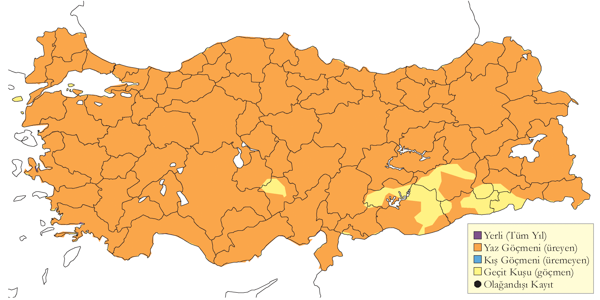
\includegraphics{images/harita_Page_043.png}

\textbf{Üreme}

\textbf{Yuvalama alanı:} Özellikle hububat tarlalarında yuvalar.\\
\textbf{Yuvası:} Ürediğini kanıtlamak son derece zordur ve Türkiye'de
henüz bir yuvası tespit edilmemiştir. Türkiye dışında, yerdeki düzce bir
çukuru ot ve yakındaki bitkisel materyal ile astarlar.\\
\textbf{Yumurta sayısı:} Genellikle 7-12, istisnai olarak 6-18 arasında
yumurta koyar.\\
\textbf{Üreme dönemi:} Genellikle nisan sonu ile mayıs ortası arasında
yumurta koyar. \textbf{MAR.} Uluabat Gölü'nde 22 Mayıs 1966'da yavrular
gözlenmiştir. Çoğu bölgeye ilkbaharda nisan ortasından gelir ve tüm
yavru gözlemleri üremenin alana varıştan hemen sonra başladığını
gösterir. Ağustos'ta duyulan kuşlar gecikmiş bir üremenin göstergesi
olabilir. \textbf{GDA.} Birecik'te 4 Haziran 1993'de tamamen palazlanmış
3 haftalık 9 yavru, hasat döneminde biçilmiş mısırın altında saklanırken
görülmüş ve köylüler tarafından yenmek üzere yakalanmıştır. 5 Haziran
1993'de görülen başka 6 kuş, yumurtlama tarihinin yaklaşık 20 Nisan'da
olduğunu gösterir. Suriye'de yavrularıyla dolaşan bir çift temmuz ayında
gözlenmiştir (Baumgart et al. 1995).

\textbf{Alttürler ve Sınıflandırma}

Türkiye'de nominat alttürü bulunur.

\section{Kınalı Keklik}\label{kux131nalux131-keklik}

\emph{Alectoris chukar}, Chukar Partridge

\textbf{\emph{Yaygın olarak çok sayıda bulunabilen bir yerli türdür.}}

Yaygın, Trakya ve Batı Karadeniz kıyı şeridinde nadir, Türkiye genelinde
ise oldukça bol bulunan yerli bir kuş türüdür. İç bölgelerde genellikle
700-2000 metre arasında görülür ve genellikle kurak, kayalık tepe ve
dağlık alanlarda, en az 2800 metreye kadar kaydedilmiştir. Hemen hemen
40 bireye kadar çıkabilen ve gençleri de içeren oldukça büyük sürüler
gözlenmiştir.

Geçmişte özellikle Hatay ve Doğu Karadeniz kıyı şeridi gibi bölgelerde
oldukça bol olarak kaydedilmiş, ancak son zamanlarda belirgin bir azalma
göstermiştir.

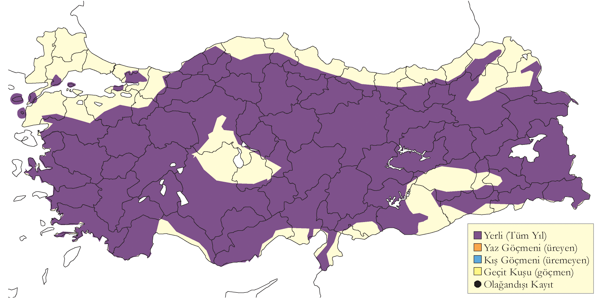
\includegraphics{images/harita_Page_039.png}

\textbf{Üreme}

\textbf{Yuvalama alanı:} Bodur çalılar ile kurumuş tarım alanlarının
bulunduğu kayalık ve taşlık tepelerle oldukça kurak ve çorak alanlarda
ürer.\\
\textbf{Yuvası:} Yerde yuvasını bir çalı ya da bitki dibine gizler.\\
\textbf{Yumurta sayısı:} Genellikle 5-22 arasında değişmekle birlikte,
bazı bölgelerde daha düşük ya da yüksek sayılarda yumurta
kaydedilmiştir.\\
\textbf{Üreme dönemi:} Genellikle mayıs sonu ile haziran başı arasında
yumurtlamaya başlar. Yavrular, temmuz ayı ortasına kadar
gözlemlenebilir. Farklı bölgelerde kaydedilen üreme dönemleri, ortam
koşullarına bağlı olarak değişiklik gösterebilir. \textbf{EGE.}
Kuluçkadaki bir ergin birey, İzmir yakınlarında 14 yumurta içeren bir
yuvadan (Ramsay 1914) 7 Mayıs 1951 tarihinde alınmıştır. Yuva, yuvanın
sahibi olan kuşun çok sayıda tüyü ile birlikte çalı benzeri bitkilerle
astarlanmış ve dikenli meşe ile de korunmuştur. Yumurtalar krem ile
kırmızı arasında bir renklenme ile kırmızımsı küçük beneklenmeler
gösterir (McNeile 1950, 1951, 1954, 1967, 1968, 1970, 1972, 1973).
\textbf{AKD.} 11 Mayıs 1899 tarihinde Acıgöl'de 5 yumurtalı bir yuva
kaydedilmiştir; dişinin yumurtlamaya devam edeceği düşünülmüştür (Selous
1900). Karadağ'da, taze yumurtalar içeren iki yuva 1907 yılının Mayıs
sonunda kaydedilmiştir. Bu yuvada taze yumurtalar haziran ayında da
bulunmuştur. Bir ergin ile 5-6 iyi gelişmiş genç birey, Burdur ve Bucak
arasındaki geçitte 13 Temmuz 1968 tarihinde kaydedilmiştir (Rokitansky
\& Schifter 1971). \textbf{İÇA.} 22 yumurta içeren bir yuva, 24 Mayıs
1998 tarihinde Ereğli yakınlarındaki bir kraterin, bir çalı ile sarılmış
kaya çıkıntısı üzerinde kaydedilmiştir. 20 yumurtadan 9 tanesi nisan ayı
sonunda bırakılmıştır (Banoğlu ve Burr 1953). \textbf{DOA.} Nemrut
Dağı'nda (Bitlis), 9 Haziran 2004 tarihinde sabah saatlerinde 15
yumurtalı bir yuva kaydedilmiştir. Ancak, günün ilerleyen saatlerinde,
ergin bir birey yuva üzerine oturmuştur. Muhtemelen bu tarih
inkübasyonun ilk günü olarak belirtilebilir. Yuva, kısmen yaprak döken
ormandaki bodur çalılar altında bulunur. Zemine derin bir şekilde
kazılmış ve birkaç adet ergin kuş tüyü ve otların kökleri ile
astarlanmıştır. \textbf{GDA.} Kuluçka kayıtları 2 Haziran 2001 tarihinde
Işıklı'da (Gaziantep) gençleri içermektedir ve 22 Haziran 1966 tarihinde
Menemen (İzmir) yakınlarında 6, 7 ve 8 yavrulu bireyleri içermektedir.
Akdeniz Bölgesi'nde 22 Mayıs 1989 tarihinde bir kuluçka ve 30 Haziran
1966'da Aladağlar'da birkaç günlük genç bir birey kaydedilmiştir. Birkaç
kuluçkanın birleşmesi sonucunda oluşan ve yaygın olarak gözlemlenmeyen
büyük kuluçkalar, tek bir ergin ile birlikte 13 Ağustos 1967 tarihinde
Kızılcahamam'da (Ankara) kaydedilmiştir (Barış et al. 1984).

\textbf{Alttürler ve Sınıflandırma}

Türkiye'nin güneyi boyunca \emph{cypriotes} alttürü görülmektedir.
Kuzeyde \emph{kleini} ve Doğu Akdeniz bölgesine özgü \emph{sinaica}
alttürünün etkili olduğu bölgede, Güneydoğu Anadolu'da
\emph{kurdestanica} alttürü bulunmaktadır. Tür içerisindeki coğrafi
varyasyon konusu ile ilgili kesin bir çıkarım yapılamamıştır; ancak
gözlemlenen formların tamamı, güçlü bir şekilde gradient ile birlikte
belirgin klinal yapı göstermektedir (Madge \& McGowan 2002).

\bookmarksetup{startatroot}

\chapter{Deniz ve Göl Kuşları}\label{deniz-ve-guxf6l-kuux15flarux131}

\section{Flamingo}\label{flamingo}

\emph{Phoenicopterus roseus}, Greater Flamingo, {[}Vinyet: Sulakalan{]}

\textbf{\emph{Lokal olarak iki alanda büyük koloniler kuran yerli bir
türdür. Kış aylarında çok daha geniş bir alana yayılır ve göçmen
kuşlarla birlikte sayıları artar.}}

Tuz Gölü ve Gediz Deltası, flamingoların Türkiye'deki iki önemli üreme
alanıdır. Tuz Gölü, onlarca yıl boyunca 10.000-20.000 çift flamingoya ev
sahipliği yaparak en önemli üreme sahası olmuştur. 1969'da Tuz Gölü'nde
ilk kez flamingoların ürediği şüphelenmiş ve yapılan araştırmalarda
gölün ortasındaki küçük bir adada yumurta kabukları bulunmuştur. Aynı
yıl 14.000 birey tespit edilmiş ve yaklaşık 1500-2000 kuşun ürediği
tahmin edilmiştir. 1970'te 5000 çiftin ürediği bir koloni bulunmuş,
ancak 1971'de su seviyesinin yüksekliği nedeniyle sadece 83 yuva
sayılmıştır. 1972'de 3500 çift, 1973'te 3700 çift, 1974'te yaklaşık 1000
yavru ve yavrularla ilgilenen 2000 erişkin birey tespit edilmiştir.
1978'de ise yaklaşık 5000 çift üreme kaydedilmiştir.

Araştırmalar 1978-1991 yılları arasında duraksamış, 1991'den itibaren
düzenli gözlemler ve hava uçuşlarıyla flamingo sayımları yapılmıştır.
1991'de yapılan bir hava gözleminde yeni bir üreme alanı bulunmuş ve
toplamda 11.000 yuva ve 4100 yavru sayılmıştır. 1992'de ise 14.000 yavru
kaydedilmiştir. Sonraki yıllarda yapılan sayımlarda 1997'de 4000,
1998'de 11.400, 1999'da 1200, 2000'de 8000-10.000, 2002'de 4750, 2003'te
3059 ve 2004'te 7312 yavru sayılmıştır. 2005'te 11.499 çift ve 3309
yavru, 2006'da 13.302 yavru, 2007'de ise 4382 yavru kaydedilmiştir.
Ancak 2007'de yaşanan kuraklık nedeniyle yüzlerce yavrunun palazlanmadan
öldüğü belirlenmiştir. 2008'de 1610 yavru, 2009'da 14.644 yavru, 2010'da
ise 5070 yavru sayılmıştır.

2011 ve 2013 yılları arasında yapılan gözlemler, Tuz Gölü'nde bugüne
kadar gözlemlenen en yüksek yavru sayısına ulaşıldığını göstermiştir:
sırasıyla 18.418, 20.274 ve 20.292 yavru. Ancak 2014 yılında bu sayı
2893'e düşmüştür. Bu düşüşün, 2007'de olduğu gibi kuraklık nedeniyle
gerçekleştiği düşünülmektedir.

Gediz Deltası'ndaki Çamaltı Tuzlası'nda flamingolar, ilk kez 1982'de
100-150 çift olarak üremeye başlamış, 1987'ye kadar üreme denemeleri
devam etmiş ancak başarı oranı çok düşük olmuştur. 1987-1991 yılları
arasında 100-200 çift düzenli olarak üremiş ve bu süreçte üreme başarısı
artmıştır. Sonraki yıllarda üreyen çiftlerin sayısı artmış, 1995 yılında
toplam 1752 çift yuvalamıştır (Sıkı 1988, Magnin \& Yarar 1997). 2000'li
yıllarda gerçekleştirilen koruma çalışmaları sonucunda flamingo kolonisi
hızla büyümüştür; 2003'te 3100 yavru, 2004'te 3000-3500 yavru, 2005'te
4025 yavru, 2006'da ise 7140 yavru yetişmiştir (Sıkı 2002, (Onmuş et al.
2011)). Ancak, üreme adalarının erozyona uğraması nedeniyle koloni
küçülmeye başlamış, 2007'de 3000-4000 yavru, 2008'de 3200 yavru, 2009'da
3000-3500 yavru ve 2010'da 2071 yavru sayılmıştır (Onmuş ve Sıkı 2011).
2011 yılında 2500-3000 çiftin üremesi, koloniye giren köpekler nedeniyle
başarısız olmuştur. Aynı yıl, deltada ilk kez Homa Lagünü'nde başarılı
bir şekilde yaklaşık 1000 yavru yetiştirilmiştir.

2012 yılında Çamaltı Tuzlası'ndaki üreme adasının kıyı erozyonuyla yok
olması üzerine bir proje başlatılmış ve 6400 m² büyüklüğünde yeni bir
üreme adası inşa edilmiştir. Flamingolar 2012 ve 2013 yıllarında bu
adayı kullanmamış, Homa Dalyanı'nda üremeye devam etmişlerdir. 2012
yılında burada 1600 yavru sayılmış, 2013 yılında 3000 çift üremeye
başlamış ancak fırtınalar nedeniyle yalnızca 130-140 yavru hayatta
kalmıştır. 2014 yılında yeni kurulan üreme adası ilk kez başarıyla
kullanılmış ve deltada bugüne kadarki en büyük koloni oluşmuştur; 10.812
çift ve 7000 yavru sayılmıştır.

1969'dan bu yana Türkiye'de toplam dokuz farklı alandan flamingoların
üreme kaydı alınmıştır. Acıgöl'de 1964 ve 1968 yıllarında üreme tespit
edilmiş (Dijksen \& Kasparek 1988), 1993'te ise en fazla 100 çiftlik bir
koloni bulunmuş ve 2006'da 100 yavru flamingo gözlenmiştir. Akşehir
Gölü, 2008 yılında tamamen kuruduğunda, kolonide 100 ölü yavru flamingo
tespit edilmiştir. 2013'te 2950-3200 çiftin ürediği gözlenmiş ancak
üreme sezonunun ilerleyen döneminde koloninin dağıldığı tespit
edilmiştir. 1960'larda, az sayıda flamingonun Ceyhan Deltası'nda
(muhtemelen Yumurtalık Lagünleri) ürediği düşünülmüştür (Warncke
1964-\/-65). Akyatan Gölü'nde 2009 yılında 163 yuvadan oluşan bir üreme
adası tespit edilmiş ancak yavru çıkarılıp çıkarılmadığı
belirlenememiştir.

Sultansazlığı'ndaki Yay Gölü'nde, 1970'te 1500-2000 çiftin ürediği
kaydedilmiş (Warncke 1971), Haziran 1974'te 8000 birey sayılmış ve 200
çiftin yuva yaptığı gözlenmiştir. Geçmişte Türkiye'deki flamingo üreme
popülasyonunun büyük bir kısmı Sultansazlığı'nda yoğunlaşmaktaydı;
bölgede ortalama 20.000-30.000 birey sayılmış, Ekim 1980'de ise istisnai
olarak 60.000-80.000 birey gözlenmiştir. Seyfe Gölü'nde 1970'te iki
küçük aktif yuva tespit edilmiş (Turan 1990), 1992'de ise 1947 yuva
sayılmış, 1993'te birkaç yüz yuva ve 1994'te 240 yavru gözlenmiştir.
Karapınar Ovası'nda 1976 ve 1977'de 500 çiftlik bir koloninin bulunduğu
düşünülmüş, ancak bu üremenin başarıyla gerçekleştiği hiçbir zaman
doğrulanmamıştır.

Ereğli Sazlığı'nda 1987'de 35-40 yuva bulunmuş, 1991'de ise 217 yuva
tespit edilmiş ancak hava gözlemlerinde koloninin terk edildiği
görülmüştür. 1993'te 300 üreyen çift ve birçok yavru gözlenmiş ancak
1991 yılından sonra en fazla 20 çiftin ürediği rapor edilmiştir.
Sazlığın 80'ler ve 90'lardaki cazibesinin artmasının, bölgenin kuruma
sürecinde tuzluluğun yükselmesinden kaynaklandığı düşünülmektedir.
Flamingoların üreme alanlarını düzensiz mesken tutması, biyolojilerinin
iyi bilinen bir özelliğidir ve bu alanlara ulaşımın zorluğu, gözlem
verilerinin düzensiz olmasına yol açmaktadır.

Erçek Gölü'nde yaz sonunda ve sonbahar başında çoğunlukla erişkinlerden
oluşan ve sayıları binleri bulan topluluklar görülür. Erçek Gölü, Sodalı
Gölü ve Van Gölü havzasındaki diğer sulakalanlarda görülen
flamingoların, muhtemelen İran'daki Urumiye Gölü'nden geldikleri
düşünülmektedir. İran'daki üreme kolonilerinde halkalanan yavru
bireyler, Türkiye'de en az 22 kez gözlenmiştir (Johnson 1989,
Behrouzi-Rad 1992).

Kış aylarında, eylül sonu ile nisan başı arasında Marmara, Ege ve
Akdeniz'deki sulakalanlarda flamingolar oldukça yaygın ve yüksek sayıda
gözlenir. Büyük çoğunluğu Gediz Deltası, Büyük Menderes Deltası, Seyhan
ve Ceyhan deltalarında toplanır. Kış Ortası Su Kuşu Sayımları'nda 1972
yılında toplam 25.900 kuş sayılmış, bunun 19.000'i Akyatan Gölü'nde
tespit edilmiştir. 1999'da toplam 51.755 kuş sayılmış, bu kuşların
18.930'u Akyatan Gölü'nde, 14.889'u Büyük Menderes Deltası'nda ve
15.413'ü Gediz Deltası'nda görülmüştür (DHKD 1999). 2002'de ise Ege
Bölgesi'ndeki Büyük Menderes ve Gediz deltalarında toplam 29.000
flamingo kaydedilmiştir (Balmer \& Betton 2003a). Flamingo kışlama
popülasyonu 2014'e kadar artış göstermiş ve ortalama popülasyon
büyüklüğü 55.000 ± 20.000 kuş olarak hesaplanmıştır. Bazı kuşlar, ılıman
kışlarda İç ve Doğu Anadolu'daki sulakalanlarda da kalabilmektedir. Ocak
1969'da Tuz Gölü'nde 1700, Sultansazlığı'nda ise 2000 flamingo
sayılmıştır.

Türkiye'de üreyen flamingoların çoğunun ülke sınırlarında kaldığı, kışın
gelen göçmen kuşlarla sayılarının arttığı düşünülse de, Türkiye'de
üreyen kuşların bir kısmı da başka ülkelere gitmektedir. 2003-2009
yılları arasında Gediz Deltası'nda yavru olarak halkalanan flamingolar,
Batı Akdeniz, Kuzey Afrika, Doğu Akdeniz ve Arap Yarımadası'nda toplam
16 farklı ülkede tespit edilmiştir. Bu kuşlardan bazıları, Gediz Deltası
dışında Fransa, İtalya ve Cezayir'deki kolonilerde başarıyla üremiştir.
Aynı şekilde, Fransa, İspanya ve İtalya'da doğan flamingolar da
Türkiye'de yıl boyunca gözlemlenmiş ve Gediz Deltası'nda başarılı
şekilde üremiştir (Johnson 1989, Balkız et al. 2009).

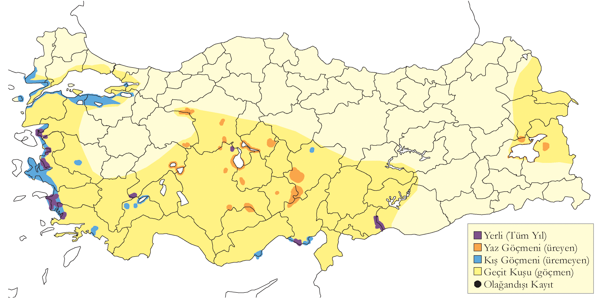
\includegraphics{images/harita_Page_056.png}

\textbf{Üreme}

\textbf{Yuvalama alanı:} Tuzlu veya aşırı tuzlu sığ göllerde koloniler
halinde yuvalar. Yuva alanları deniz seviyesinden 1100 metre rakıma
kadar çıkabilir. Türkiye'deki kolonilerdeki kuş sayısı 100 ile 23.000
arasında değişmektedir.\\
\textbf{Yuvası:} Koloni, sığ suda, alçak bir adaya veya kurumuş bir
çamur düzlüğüne kurulur. Yuva, çamurdan yapılmış kesik bir koni
şeklindedir; genellikle 25-40 cm, nadiren 10 cm yüksekliğinde olur ve
ters çevrilmiş bir saksıya benzer. Zamanla kuruyarak son derece sert bir
hal alır. Yuvanın ortası çukurdur ve zeminine tüyler eklenebilir.\\
\textbf{Yumurta sayısı:} Tek bir yumurta bırakır.\\
\textbf{Üreme dönemi:} Yumurtlama dönemi nisan başı ile haziran ortası
arasındadır. Yumurtlama tarihi, alandaki su seviyesiyle ilişkili
olabilir. Kuşlar, üreme döneminde oldukça hassastır ve rahatsızlık
nedeniyle tüm koloniyi terk edebilirler. Yuvayı terk eden kuşlar o yıl
başka bir yerde tekrar yuva kurmaz ve yumurta bırakmaz. \textbf{EGE}.
Gediz Deltası'ndaki tuzlalarda 1995 yılında 1450 çift flamingonun
ürediği gözlenmiş, koloni 15 Mart'ta oluşmaya başlamış ancak mayıs
sonunda terkedilmiştir (Eken 1997a). \textbf{İÇA}. Tuz Gölü,
flamingoların en düzenli ürediği ve en büyük kolonilere ev sahipliği
yapan aşırı tuzlu bir göldür. Burada 31 Mart 1969'da kur ve çiftleşme
davranışları kaydedilmiştir (Warncke 1971). 18 Mayıs 1970'te bulunan
5000 yuvanın \%70'inde yumurta, 20'sinde yavru, 10'unda ise boş yuvalar
gözlenmiştir. Bu, üremenin nisan başında başladığını gösterir (Warncke
1971). 24 Mayıs 1972'de neredeyse her yuvada bir haftalık yavrular
görülmüştür. 15 Haziran 1973'te 1-3 haftalık yavrular kaydedilmiş, bu da
yumurtlamanın nisan ortasında başladığını göstermiştir. 11 Haziran
1974'te 30-40 günlük yavrular gözlemlenmiş, yumurtlamanın nisan başında
başladığını doğrulamıştır (Kahl 1975). 6 Temmuz 1992'de gözlenen
1000-2000 yavrunun yaklaşık 4 haftalık olduğu tahmin edilmiştir. Haziran
1992'de yapılan havadan sayımda gölün güneyindeki koloninin yeri tespit
edilmiş ve yürüyen yavruların koloniden 2-5 kilometre uzakta olduğu
görülmüştür (Magnin \& Yarar 1997). Seyfe Gölü'nde 18-22 Haziran 1992
tarihleri arasında en büyüğü 15 günlük yavrular gözlenmiş, bu da
yumurtlamanın mayıs başında başladığını göstermektedir. 1993'te 13
Mayıs'ta yapılan gözlemde kolonideki yuvaların çoğunun eski olduğu, 14
Haziran'da ise 200-500 yeni yuvanın yapıldığı ve çoğunun çamurunun henüz
kurumadığı tespit edilmiştir. Bu yuvalardan yaklaşık 20 tanesinde
yumurta bulunmuş ve üremenin yeni başladığı anlaşılmıştır. Aynı yıl,
70-80 flamingo yuvası üzerine bir ak pelikan kolonisinin yerleştiği
gözlenmiştir. Ereğli Sazlığı'nda 10 Mayıs 1987'de önceki yıla ait olduğu
düşünülen 35-40 yuva bulunmuş, 1 Haziran 1991'de üç küçük adada 1100
erişkin ve 227 yuva sayılmış, bunlardan sadece 68'inde yumurta tespit
edilmiştir (Kirwan 1992a). 16-17 Haziran 1993'te yapılan sayımda dört
adada 300 çiftin ürediği, 17'sinin boş, 54'ünün yumurtalı ve 33'ünün ise
en büyüğü bir haftalık yavrulara sahip olduğu belirlenmiştir (Magnin \&
Yarar 1994). Yumurtlama en erken 10 Mayıs'ta başlamıştır.
Sultansazlığı'nda 8-10 Haziran 1974'te 200 çiftin yuvalamaya henüz
başladığı gözlenmiştir (Kahl 1975).

\textbf{Alttürler ve Sınıflandırma}

Monotipik bir türdür.

\section{Küçük Flamingo}\label{kuxfcuxe7uxfck-flamingo}

\emph{Phoeniconaias minor}, Lesser Flamingo, {[}Vinyet: Sulakalan{]}
{[}Vinyet: Rastlantısal{]}

\textbf{\emph{Rastlantısal konuktur.}}

10-16 Nisan 2006'da Ereğli Sazlığı'nda bir flamingo grubunun içinde
tespit edilen kuş, Türkiye'deki ilk kaydı oluşturmuştur. Benzer
tarihlerde İsrail'de de kaydedilmesi, bu kuşun yabani olduğu iddiasını
desteklemiştir. Ardından 30 Ocak - 30 Nisan 2009'da Gediz Deltası'nda, 3
Haziran 2009'da Kulu Gölü'nde, 22 Nisan 2011'de Kulu Gölü'nde, 21 Ocak
2012'de Enez Lagünleri'nde, 15 Nisan ve 18 Haziran'da ve sonrasında 24
Ekim - 2 Kasım 2012 arasında Kulu Gölü'nde, 26 Nisan ve 11 Mayıs 2014'te
ve 2015 yılında yine Kulu Gölü'nde görülmüştür.

İspanya ve Fransa'da yabani olduğu düşünülen kuşlar defalarca gözlenmiş,
Güneybatı Moritanya'da en az bir kez üremiştir. Avrupa'daki bazı
kayıtlar doğal yaşam parklarından kaçan kuşlara ait olabilir.

\textbf{Üreme}

Türkiye'de ürememektedir. Yayılış alanı Sahra altı Afrika'dır.

\textbf{Alttürler ve Sınıflandırma}

Monotipik bir türdür. Bu tür bazen Phoenicopterus cinsi altına
yerleştirilir.

\section{Küçük Batağan}\label{kuxfcuxe7uxfck-bataux11fan}

\emph{Tachybaptus ruficollis}, Little Grebe, {[}Vinyet: Sulakalan{]}

\textbf{Yaygın ve çok sayıda bulunan yerli bir türdür. Kışın ve göç
döneminde sayıları artar.}

Bataklık sulakalanlarda nispeten az sayıda ürer. Üreme sonrası
toplanmalara temmuzdan itibaren tüm bölgelerde rastlanır. Genellikle
300-500 kuşluk sürüler gözlenirken, Manyas, Erçek ve Van göllerinde
1000'den fazlası toplanabilir. En yüksek sayı Eylül 2000'de Sarıyar
Barajı'nda kaydedilen 2625 kuştur.

Kışın çoğunlukla batı ve orta kesimlerdeki tatlı su gölleri,
bataklıklar, göletler, kıyısal sulakalanlar ve az sayıda denizde
görülür. En yüksek sayılara batı ve güney bölgelerinde, özellikle Bafa
Gölü, Büyük Menderes Deltası, Köyceğiz Gölü ve Göksu Deltası'nda
rastlanır. Marmara Bölgesi'nde kışın yaygındır. 3 Şubat 1991'de
Küçükçekmece Gölü'nde 1120 birey sayılmıştır. Zonguldak Ereğli'de,
kuşların ekim ayının ikinci yarısında gelip mart sonuna kadar kaldıkları
gözlenmiştir. İç Anadolu ve Doğu Anadolu'dakiler kışın Ege ve Akdeniz
bölgelerine iner, mart ayında üreme bölgelerine geri dönerler. İç
Anadolu ve Göller Bölgesi'nde ılıman geçen kışlarda yüksek sayılarda
toplanır. 11 Şubat 2005'te Sarıyar Barajı'nda 538, 20 Ocak 2005'te
Eğirdir Gölü'nde 1155 birey sayılmıştır.

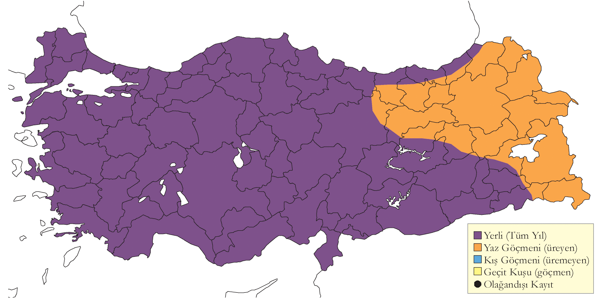
\includegraphics{images/harita_Page_051.png}

\textbf{Üreme}

\textbf{Yuvalama alanı:} Sık bitkilerle kaplı tatlı ve acı göller,
bataklıklar, aynası olan sazlıklar ve eski nehir yataklarında ürer.
Üremesi ve yuvalaması için yeterli bitki örtüsü olduğu sürece çok küçük
göletleri bile kullanabilir.\\
\textbf{Yuvası:} Genellikle canlı bitkilere tutunan yüzer yuva yapar.
Yuva, sucul bitkiler öbeğinden oluşur ve ortasında hafif bir çukur
vardır.\\
\textbf{Yumurta sayısı:} Türkiye'de gözlenen yumurta sayısı 4-5
arasındadır. Türkiye dışında ise yumurta sayısı çoğunlukla 4-6, istisnai
olarak 2-7 olur. Gözlenen yavru sayısı dağılımı şu şekildedir: 2 yuvada
1, 4 yuvada 2, 2 yuvada 3, 2 yuvada 4, 1 yuvada 5 yavru. Daha düşük
yavru sayıları, kayıplardan kaynaklanır.\\
\textbf{Üreme dönemi:} Üreme dönemi mart ayında başlar ve bölgeye göre
değişiklik gösterir. İlk yumurtalar genellikle nisan başında ortaya
çıkar ve üreme ağustos ayına kadar devam eder. \textbf{MAR}. En erken
yavru 4 Haziran 1996'da İstanbul Belgrad Ormanı'nda görülmüştür. 2
Haziran 2006'da Uluabat Gölü'nde bir yuvada beş yumurta bulunmuştur.
\textbf{KAR}. Kızılırmak Deltası, tür için en önemli üreme alanıdır.
1992 yılında üreme popülasyonunun 350-500 çift olduğu tahmin edilmiş ve
seyrek koloniler halinde ürediği, üreme sıklığının 100 hektarda 25-45
çift olduğu belirlenmiştir (Hustings \& Dijk 1994). İki yetişmiş yavru
10 Haziran 1995'te, dört yavru ise 15 Temmuz 1971'de görülmüş, 1992
yılındaki kapsamlı araştırmada ilk yavruya 26 Mayıs'ta rastlanmıştır
(Dijksen \& Kasparek 1985, Hustings \& Dijk 1994). \textbf{EGE}. 5 Mayıs
1995'te Bafa Gölü'nde gözlenen dört yavru, yumurtlama tarihinin nisan
başı olduğuna işaret eder. \textbf{AKD}. Çukurova'da en erken gözlem, 4
Mayıs 1987'de hav tüyleri bulunan bir yavru olmuştur (Van der Have vd.,
1988). 18 Mayıs 1970'te Antalya çevresinde büyümüş yavrular
gözlenmiştir. \textbf{İÇA}. 18 Mayıs 1998'de Uyuz Gölü'nde ve 19 Mayıs
1998'de Eşmekaya'da dörder yumurtalı yuvalar tespit edilmiştir.
Sultansazlığı'nda karayoluna paralel uzanan kanal boyunca erişkinlerin
kuluçkaya yattıkları gözlenmiş, 14 Mayıs 2004'te bir yuvada beş yumurta
görülmüştür. 8 Ağustos 1971'de Akşehir Gölü'nde kuluçkada erişkinler
gözlenmiştir. Sultansazlığı'nda en erken yavru 7 Haziran 1982'de
kaydedilmiştir (Kasparek 1985). \textbf{DOA}. 19 Haziran 2004'te Erçek
Gölü'nde yumurtlama süreci devam eden bir yuvada iki yumurta bulunmuş,
bir başka yuvada ise yeni çıkmış iki yavru gözlenmiştir. 18 Ağustos
1972'de Sodalı Göl'de hala kuluçkada olan bir erişkin gözlenmiş ve 25
Haziran'dan itibaren yedi farklı yavru gözlemi kaydedilmiştir. Geç
tarihli kayıtların muhtemelen ikinci kuluçka ile ilgili olduğu
düşünülmektedir. \textbf{GDA}. 7 Haziran 2006'da Birecik'te yumurtadan
yeni çıkmış bir yavru görülmüştür.

\textbf{Alttürler ve Sınıflandırma}

Batı Anadolu'da nominat \emph{ruficollis} alttürü bulunur. Doğu
Anadolu'da \emph{capensis} alttürü olabileceği iddia edilmiştir
(Roselaar 1995). Avrupalı ruficollis ve Afro-Asyalı \emph{capensis} ve
\emph{albescens} alttürlerinin göz renginin farkıyla rahatlıkla tespit
edilebileceğini belirtmiştir (Swelm 2001). Dolayısıyla Roselaar'ın
varsaydığı alttür, \emph{albescens}, hatta Irak'ta bulunan
\emph{iraquensis} olabilir. Doğu Anadolu'daki kuşların hangi alttüre ait
olduğu kesinleştirilmelidir.

\section{Kulaklı Batağan}\label{kulaklux131-bataux11fan}

\emph{Podiceps auritus}, Horned Grebe (Slavonian Grebe), {[}Vinyet:
Sulakalan{]} {[}Vinyet: VU (2016){]}

\textbf{\emph{Nadir bir kış konuğudur.}}

Karadeniz ve Marmara kıyılarında eylül sonu ile mayıs başı arasında
nadiren rastlanır. 2008'e kadar 21 bilinen kaydı vardır. 2 Ekim 1972'de
Küçükçekmece açıklarında görülen 6 kuş en kalabalık gruptur. Zonguldak
Çatalağzı açıklarında, bir kara boyunlu batağanla birlikte görülen kuş,
şubat sonundan 11 Mart 1948'e kadar konaklamıştır.

Karadeniz ve Marmara kıyıları dışında çok nadir görülür. 29 Ocak 1997'de
Balıkesir Ören'de dört kuş, şubat 1989'da Göksu Deltası'nda bir kuş, 22
Nisan 1999'da Diyarbakır Çınar-Göksu Barajı'nda bir kuş, 27 Ocak 2008'de
Sarıyar Barajı'nda ve 27 Ocak 2014'te Sapanca Gölü'nde birer kuş
gözlenmiştir.

Tek bir yaz kaydı vardır: Üreme giysisindeki bir kuş, 1 Temmuz 1985'te
Çaldıran'da gözlenmiştir.

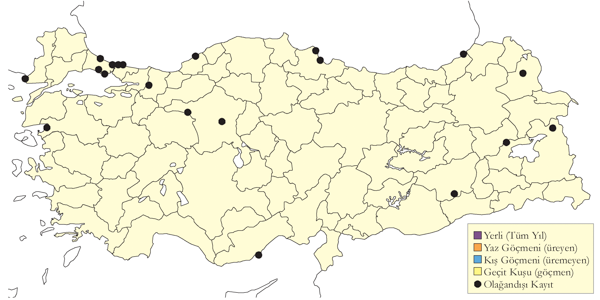
\includegraphics{images/harita_Page_054.png}

\textbf{Üreme}

Türkiye'de ürememektedir. Üreme dönemindeki yayılış alanı K. Avrasya,
Kanada ve K. ABD'dir.

\textbf{Alttürler ve Sınıflandırma}

Monotipik bir türdür.

\section{Kızıl Boyunlu Batağan}\label{kux131zux131l-boyunlu-bataux11fan}

\emph{Podiceps grisegena}, Red-necked Grebe, {[}Vinyet: Sulakalan{]}

\textbf{\emph{Lokal olarak ve az sayıda bulunan bir yaz konuğu, yaygın
ancak nadir bulunan bir geçit türü ve kış konuğudur.}}

İç Anadolu'da Ereğli Sazlığı ve Sultansazlığı gibi büyük sulakalanlarda,
Doğu Anadolu'da ise küçük ve bataklık sulakalanlarda yuvalar, deniz
seviyesinden 2250 metre yüksekliğe kadar çıkar. Bu tip küçük
sulakalanlar nadiren ziyaret edildiğinden, gözlem kayıtlarının
oluşturduğu izlenimden daha yaygın olabilir. Üreme alanlarına martın
üçüncü haftasında gelir ve ekim sonuna kadar kalır. Üremeyen veya
üremesi başarısız olan bireyler yazın küçük topluluklar oluşturabilir.
Temmuz 2001'de Sodalı Göl'de 40 birey, 9 Haziran 1998'de Eşmekaya
Sazlığı'nda 73 kuş (Eken \& Magnin 1999) toplanmıştır.

Kışın Marmara ve Karadeniz bölgelerinde az sayıda, nadiren içsularda
görülür. Ocak 1970'de 10, 1-3 Eylül 1980'de Burdur Gölü'nde 150 birey
sayılmıştır.

Yirminci yüzyılın ilk yarısından gelen kayıtlar, bu türün eskiden daha
yaygın olduğunu göstermektedir. 1945-46 yıllarında Mogan Gölü'nde
yaklaşık 20 çift üremiştir. Ancak Mogan Gölü'ndeki son üreme 1998
yılında kaydedilmiştir. Son yıllarda sulakalanların kurutulması
nedeniyle İç Anadolu'da sayıları azalmıştır.

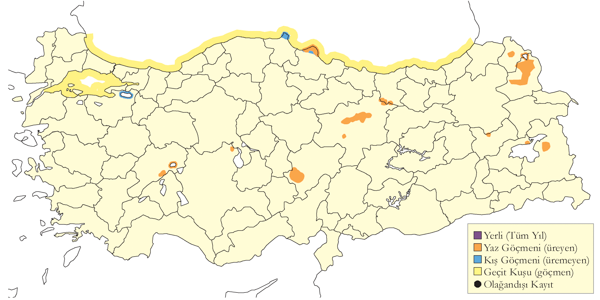
\includegraphics{images/harita_Page_052.png}

\textbf{Üreme}

\textbf{Yuvalama alanı:} Kenarları sazlık göller, bataklıklar ve göl
aynası olan sazlıklarda ürer.\\
\textbf{Yuvası:} Çoğunlukla büyüyen bir bitkiye tutturulmuş yüzer
yuvası, çürümüş su bitkilerinden oluşur ve ortasında çukur olan alçak
bir yapıdır.\\
\textbf{Yumurta sayısı:} Türkiye'de tek bir yuvada 3 yumurta görülmüş,
Türkiye dışında yumurta sayısı genellikle 4-5 arasındadır. Gözlenen
yavru sayısı çoğunlukla 1, nadiren 3'tür.\\
\textbf{Üreme dönemi:} Üreme nisan sonu ile mayıs başında başlar,
yumurtlama mayıs ayında gerçekleşir. Yavrular haziran ayında çıkar ve
temmuz ile ağustos aylarında gelişimlerini tamamlayarak yuvadan ayrılır.
\textbf{AKD}. 12 Nisan 1973'te Karamık Gölü'nde kur davranışı
gözlenmiştir. \textbf{İÇA}. Çeşitli alanlarda nisan sonu ile mayıs
başında kur davranışı gözlenmiştir. 27 Mayıs 1993'te Eşmekaya'da bir
yumurtalı bir yuva, 20 Mayıs 1998'de ise iki yumurtalı bir yuva görülmüş
ve yumurtlama sürecinin devam ettiği düşünülmüştür. Aynı alanda 21
Haziran 1998'de gelişmiş bir yavru gözlenmiştir. Ereğli Sazlığı'nda 19
Mayıs 1971'de 3 yumurtalı bir yuva bulunmuştur. 13 Temmuz 1977'de
Akşehir Gölü'nde, 17 Temmuz 1986'da Kulu Gölü'nde yavrular
kaydedilmiştir. Sultansazlığı'nda 1982'nin ağustos sonunda yavrulara
rastlanmıştır (Kasparek 1985). \textbf{DOA}. 29 Mayıs 1969'da Van
yakınında ve 1 Haziran 1990'da Çaldıran Gölü'nde yuva yapımına
rastlanmıştır. Kars yakınlarındaki bir alanda 18 Temmuz 1992'de yuva
yapımı gözlenmiş ve 27 Haziran itibarıyla toplam 6 yavru kaydedilmiştir.

\textbf{Alttürler ve Sınıflandırma}

Türkiye'de nominat alttürü bulunur.

\section{Bahri}\label{bahri}

\emph{Podiceps cristatus}, Great Crested Grebe, {[}Vinyet: Sulakalan{]}

\textbf{Yaygın olarak ve çok sayıda bulunan bir yerli tür ve kış
konuğudur.}

Ülke genelinde yaygın olsa da, İç Anadolu'nun geniş bataklık
sulakalanlarında ve Doğu Anadolu'da en çok sayıda miktarda bulunur.
Uluabat Gölü'nde 400 çift, Kızılırmak Deltası'nda 250-300 çift
üremektedir. Küçük batağanın tercih ettiği küçük gölet ve bataklıkları
kullanmaz ancak baraj göllerini sıkça kullanır.

Üreme dönemi sonrasında ve kışın daha yaygındır, yüksek sayılarda
görülür. Kışlayan bireyler ekim başında gelir ve nisan sonuna kadar
kalırlar. Kıyısal bölgelerde, Kızılırmak ve Yeşilırmak deltaları,
Küçükçekmece Gölü, Büyük Menderes Deltası'nda yoğunlaşır. Bu alanlarda
sert geçen kışlarda binlercesine rastlanabilir. Karadeniz kıyılarında
yüksek sayılarda gözlenmiştir. Büyük baraj gölleri önemli sayılar
barındırır; Sarıyar'da 5500, Karakaya'da 12.000 ve Keban'da 10.000 kuş
sayılmıştır. Kış Ortası Su Kuşu Sayımları'nda, 2005 yılında sayılan
yaklaşık 31.000 kuş en yüksek değerdir.

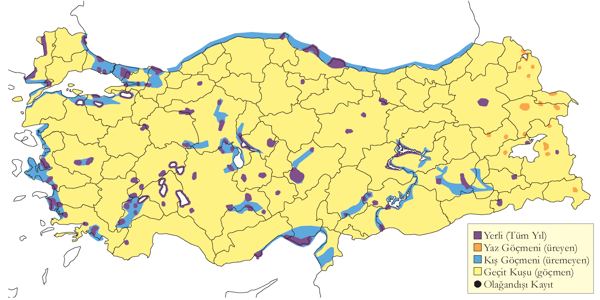
\includegraphics{images/harita_Page_053.png}

\textbf{Üreme}

\textbf{Yuvalama alanı:} Kıyılarında sazlar olan göllerde yuvalar.
Genellikle sazlara, nilüferlere ve su altındaki dallara yuvalarını
kurar. Sığ sularda yuva su tabanına oturtulurken, daha derin sularda
yüzer yuva bir bitkiye iliştirilir.\\
\textbf{Yuvası:} Yuva, sucul bitkilerden oluşan alçak bir öbek
şeklindedir ve ortasında sığ bir çukur bulunur. Nilüferler veya sazlar
gibi bitkilere tutturulmuş yüzer yuvalar yaygındır.\\
\textbf{Yumurta sayısı:} Türkiye'de gözlenen yumurta sayısı 4-5 arasında
değişir. Gözlenen yavru sayısı ise 1 ila 5 arasında kaydedilmiştir.\\
\textbf{Üreme dönemi:} Yumurtlama mart sonunda başlar ve haziran sonuna
kadar yavrular yuvadan ayrılabilir. Yuva yapımı nisan sonuna kadar devam
edebilir (Welch \& Welch 1998b). \textbf{MAR}. Uluabat Gölü'nde ortalama
yavru sayısı 2,6 (231 yuvada) olarak tespit edilmiştir (Welch \& Welch
1998b). 25 Nisan 2003'te kuluçkaya yatan birçok çift ve 19 Haziran
1999'da yetişmiş yavruyla dolaşan çiftler gözlenmiştir. 13 Mayıs 2007'de
yaklaşık 3 haftalık yavrulara rastlanmış ve yumurtlamanın mart sonunda
gerçekleştiği düşünülmüştür. Yuva yapımı 25 Nisan 1970'te gözlenmiş, 2
Haziran 1967'de biri dört, diğeri beş yumurtalı iki yuva bulunmuştur. 23
Nisan 1966'da yumurtlama süreci devam eden üç yuva tespit edilmiş, 24
Mayıs 1966'da sezonun ilk yavrusu gözlenmiştir. İznik Gölü'nde 6 Haziran
1966'da çok küçük yavrusu olan dört çift gözlenmiştir. \textbf{EGE}. 13
Mayıs 1899'da yaklaşık 20 yuva tespit edilmiş ve 21 Mayıs ile 21 Eylül
arasındaki geniş dönemde yavrular gözlenmiştir (Selous 1900).
\textbf{KAR}. Kızılırmak Deltası'nda 27 Nisan 1992'de yumurtalı yuvalar
tespit edilmiş ve ilk yavrular 20 Mayıs'ta gözlenmiştir (Hustings \&
Dijk 1994). \textbf{AKD}. Beyşehir Gölü'nde 1 Mayıs 1967'de yuva yapımı
tespit edilmiş, 10 Haziran'dan itibaren yavrular görülmüştür. Göksu
Deltası'nda 14 Eylül 1972'de sekiz uçamayan iri yavru gözlenmiştir.
\textbf{İÇA}. Hotamış Gölü'nde nisan sonundan itibaren kuluçkaya
yatılmıştır (Kirwan 1993a). Diğer alanlarda en erken yavru 6 Haziran'da
gözlenmiştir. \textbf{DOA}. Van Gölü'nde temmuz ortasında kuluçkaya
yatan erişkinler ve 8 Haziran 1975'te ilk yavrular tespit edilmiştir. Bu
durum, yumurtlamanın mayıs başında gerçekleştiğini göstermektedir.

\textbf{Alttürler ve Sınıflandırma}

Türkiye'de nominat alttürü bulunur.

\section{Kara Boyunlu Batağan}\label{kara-boyunlu-bataux11fan}

\emph{Podiceps nigricollis}, Black-necked Grebe (Eared Grebe),
{[}Vinyet: Sulakalan{]}

\textbf{\emph{Lokal olarak bulunan bir yaz konuğu, yaygın ve nispeten
çok sayıda görülen bir geçit türü ve kış konuğudur.}}

Üreme alanlarında nisan ortasından ağustos ayına kadar bulunur.
Koloniler halinde ürer, yüzlerce çift bir arada görülebilir. İç
Anadolu'da oldukça nadirdir. Son zamanlarda, örneğin Kulu Gölü'nde
(Richardson 2003), sayıları ciddi şekilde azalmıştır. Doğu Anadolu'da
2500 metre rakıma kadar olan, genellikle küçük, ötrofik ve bataklık
sulakalanlarda ürer. Kars Kuyucuk Gölü'nde 330 çift bulunur. Üremede
başarısız olan bireyler temmuz ayında gözde sulakalanlarda toplanır. Bu
topluluklara sonraki iki ay boyunca üremeyi bitiren bireyler ve ülke
dışından gelenler katılır. Bu gruplar birkaç bini bulabilir. Örneğin
Acıgöl'de 1800, Kulu Gölü'nde 2000, Erçek Gölü'nde 9 Eylül 2000'de
10.000 kuş (Birding World 1998) ve Sodalı Göl'de 4000-5000 kuş
kaydedilmiştir. Doğu Anadolu'da bu tüy döküm alanlarında aralık başına
kadar kalabilirler.

Önemli sayılarda kışlar. Karadeniz ve Marmara kıyılarında, lokal olarak
korunaklı koylar ve limanlarda ekim ortası ile nisan ortası arasında
düzenli olarak görülür (Albrecht 1986). Kışlama bölgelerinde mayıs
başına kadar kalabilir. Yüksek sayılarda Göller Bölgesi'nde bulunabilir.
Burdur Gölü'nde düzenli olarak 5000 birey, Ocak 1970'de ise 18.662 birey
sayılmıştır. İç Anadolu'da az sayıda kışlar. Son yıllarda yapılan Kış
Ortası Su Kuşu Sayımlarında, ülke toplamı 2000 kuşun altına inmiştir.

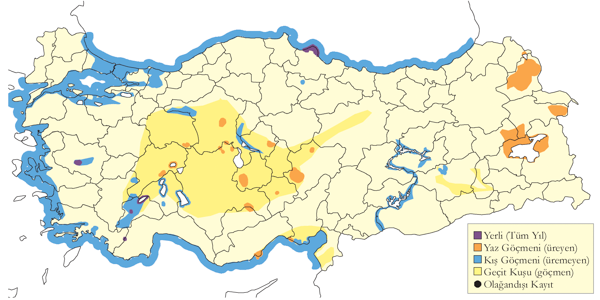
\includegraphics{images/harita_Page_055.png}

\textbf{Üreme}

\textbf{Yuvalama alanı:} Sazlıkların ve sualtı bitkilerinin bulunduğu
sığ tatlı veya acı göllerde yuvalar. Genellikle küçük koloniler
oluşturur, ara sıra tek başına da ürer.\\
\textbf{Yuvası:} Yüzer yuvası bir sucul bitkiye iliştirilir. Yuva, sucul
bitkilerden oluşan alçak bir öbektir ve ortasında sığ bir çukur
bulunur.\\
\textbf{Yumurta sayısı:} Türkiye'de gözlenen yumurta sayısı 1 ile 6
arasında değişir. Yumurta sayısının dağılımı, 16 yuvada 1, 11 yuvada 2,
8 yuvada 3, 5 yuvada 4, 1 yuvada 5 ve 1 yuvada 6 adet olarak
kaydedilmiştir.\\
\textbf{Üreme dönemi:} Üreme nisan ortasında başlar. Yavruların çıkışı
genellikle mayıs sonu ile haziran ayı arasında gerçekleşir, büyümüş
yavrular ise temmuz ayında gözlenir. \textbf{MAR}. Uluabat Gölü'nde 20
Haziran 1999'da 1-2 haftalık yavrularını gezdiren birkaç çift gözlenmiş
ve yumurtlama tarihinin 21 Mayıs civarında olduğu tahmin edilmiştir.
\textbf{KAR}. Kızılırmak Deltası'nda Mayıs 1992'de kur davranışı tespit
edilmiş, 11 Mayıs'ta bir kuşun, muhtemel bir yuvadan kalkan düşmanı
alandan uzaklaştırma davranışı gösterdiği gözlenmiştir (Hustings \& Dijk
1994). \textbf{AKD}. Çukurova sulakalanlarında 14 Nisan 1987'de kur
davranışı görülmüş, Karamık Gölü'nde 18 Temmuz 1972'de yavrusu olan iki
çift ve 29 Temmuz 1972'de Seyhan Barajı'nda üç yavrulu bir erişkin
gözlenmiştir. \textbf{İÇA}. Kulu Gölü'nde 13-15 Temmuz 1971'de yüzen su
bitkilerinden oluşan bir adanın kenarında 120 yuva tespit edilmiş, 42
yuvada yumurta bulunmuş, geri kalan yuvalardaki yavruların yuvayı terk
ettiği düşünülmüştür. 22 Temmuz 1971'de Kulu Gölü'nde 13 yuvada 1-4
yumurta sayılmış, bir yanda yüzen yavrular, diğer yanda yuva yapan
erişkinler gözlenmiştir (Kasparek 1987). Mogan Gölü'nde nisan başından
itibaren yaz konuğu olup, nisan ortasında çiftleşme ve kur davranışları
gözlenmiştir (Wadley 1951). Hotamış Gölü'nde iki koloni toplam 20-25
çiftten oluşmuştur (Kirwan 1993a). Çöl ve Uyuz Gölleri'nde 5 çiftin kur
yaptıkları 1 Haziran 1991'de gözlenmiş, 5 Temmuz 1991'de iki yavrulu bir
çift tespit edilmiştir. En erken yavru kaydı ise 31 Temmuz'dadır.
\textbf{DOA}. Kuyucuk Gölü'nde 18 Temmuz 1992'de 196 yuva sayılmış,
2000'li yıllarda bu sayı 330 çift olmuştur. Diğer alanlarda en erken
yavru kaydı 19 Temmuz'dadır.

\textbf{Alttürler ve Sınıflandırma}

Türkiye'de nominat alttürü bulunur.

\section{Kızıl Gerdanlı
Dalgıç}\label{kux131zux131l-gerdanlux131-dalgux131uxe7}

\emph{Gavia stellata}, Red-throated Loon, {[}Vinyet: Deniz{]}

\textbf{\emph{Nispeten yaygın ancak az sayıda bulunan bir kış
konuğudur.}}

Ekim sonu ile haziran başı arasında az sayılarda Orta ve Doğu Karadeniz
kıyılarında görülür. İstisnai olarak kalabalık gruplar oluşturabilir. 20
birey 9 Ocak 1969'da Yeşilırmak ağzında ve 24 birey 23 Şubat 2008'de
Kızılırmak Deltası açıklarında gözlenmiştir.

Üremeyen bireyler ilkbahar sonunda ve yazın genellikle Karadeniz
kıyılarında, daha nadir olarak iç bölgelerde bulunur. Bir birey 14
Haziran 1977'de Van Gölü kıyısında, Ahlat'ta (Beaman 1986), yaz
giysisinden tüyleri kalmış bir birey ise 16 Temmuz 2003'te Tödürge
Gölü'nde (Sivas) gözlenmiştir.

Büyük ihtimalle İstanbul çevresinden toplanmış iki tahnit, İstanbul'da
Saint Joseph Müzesi'nde sergilenmektedir (Kirwan 1997b).

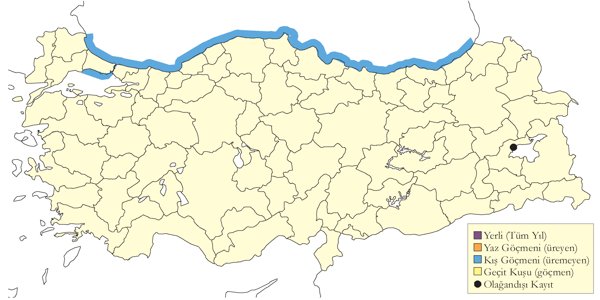
\includegraphics{images/harita_Page_045.png}

\textbf{Üreme}

Türkiye'de ürememektedir. Üreme dönemindeki yayılış alanı K. Kuzey
Amerika ve K. Avrasya'dır.

\textbf{Alttürler ve Sınıflandırma}

Monotipik bir türdür.

\section{Kara Gerdanlı Dalgıç}\label{kara-gerdanlux131-dalgux131uxe7}

\emph{Gavia arctica}, Black-throated Loon, {[}Vinyet: Deniz{]}

\textbf{\emph{Karadeniz'de çok sayıda, diğer denizlerde az sayıda
bulunan bir kış konuğudur.}}

Karadeniz ve Marmara kıyılarında eylül başı ile nisan arasında yaygın ve
bol bulunan bir kış konuğudur. Özellikle Orta ve Doğu Karadeniz'de en
yüksek sayılarda rastlanır. Kışlama döneminin sonlarına doğru Karadeniz
kıyısındaki kuşların sayısı, güneyden gelenlerin toplanmasıyla artar ve
şubat sonu ile nisan başı arasında zirve yapar. Artvin açıklarında 25-27
Ocak 1967'de 1500, 26 Şubat 2006'da 2100 birey kaydedilmiştir.
Yeşilırmak Deltası açıklarında 9-10 Ocak 1969'da saatte 50 bireyin
batıya uçtuğu görülmüştür. Ege ve Akdeniz kıyılarında oldukça seyrektir,
Göksu Deltası, Çukurova sulakalanları ve Hatay'da ise nadir görülür.
İçsularda nadiren rastlanır; 1996'da Ankara Bayındır Barajı, Haziran
1965'te Burdur Gölü, Haziran 2005'te Aygır Gölü ve Akdeniz kıyısında
rastlanmıştır.

Üremeyen kuşlar nadiren Orta ve Doğu Karadeniz kıyılarında yaz aylarında
görülebilir, bazı bireylerde kur davranışı bile gözlenmiştir. Van
Gölü'nde Haziran 1978, Haziran 1983, Temmuz 1987 ve Temmuz 1995'te
görülmüş, son kayıt suyun sodalı özelliği nedeniyle tüyleri beyazlaşmış
bir bireye aittir.

\includegraphics{images/harita_Page_046.png}

\textbf{Üreme}

Türkiye'de ürememektedir. Üreme dönemindeki yayılış alanı K. Avrasya ve
B. Alaska'dır.

\textbf{Alttürler ve Sınıflandırma}

Türkiye'de nominat alttürü bulunur.

\section{Buz Dalgıcı}\label{buz-dalgux131cux131}

\emph{Gavia immer}, Great Northern Loon, {[}Vinyet: Deniz{]} {[}Vinyet:
Rastlantısal{]}

\textbf{\emph{Rastlantısal konuktur.}}

Dört güncel kaydı bulunmaktadır. Yaz giysisinde bir kuş, 13 Mayıs
1964'te İstanbul Büyükçekmece açıklarında gözlenmiştir (Warncke
1964-\/-65). 29 Nisan 1968'de aynı bölgede, bazıları üreme giysisine
girmeye başlamış toplam 8 kuş kaydedilmiştir (Groh 1968). 27 Mart
1981'de Tekirdağ Şerefli Deresi ağzında bir birey görülmüş (Goriup \&
Parr 1983), 13 Mayıs 1989'da Göksu Deltası'nda ölü bir kuş bulunmuştur
(Kirwan \& Martins 1994).

İstanbul Robert Kolej'de bulunduğu söylenen bir tahnitin (Mathey-Dupraz
1920--24, Kasparek 1990), 1996'daki envanter çalışmasında bulunamadığı
belirtilmiştir (Kirwan 1997b). Ancak, Robert Kolej'deki birçok tahnitin
1992'den sonra zarar gördüğü veya yok olduğu bilinmektedir. Şans eseri,
Kasparek 1986'daki ziyaretinde bu tahnitin bir fotoğrafını çekmeyi
başarmıştır.

\includegraphics{images/harita_Page_047.png}

\textbf{Üreme}

Türkiye'de ürememektedir. Üreme dönemindeki yayılış alanı K. Kuzey
Amerika ve K. Avrasya'dır.

\textbf{Alttürler ve Sınıflandırma}

Monotipik bir türdür.

\section{Fırtınakırlangıcı}\label{fux131rtux131nakux131rlangux131cux131}

\emph{Hydrobates pelagicus}, European Storm Petrel, {[}Vinyet: Deniz{]}

\textbf{\emph{Ege ve Akdeniz sularında nadir rastlanan bir yaz
konuğudur.}}

Yakın zamana kadar yalnızca birkaç kaydı bulunan nadir bir konuk olduğu
düşünülmekteydi. Ancak, 6 Ağustos 2010'da Didim açıklarında iki kuş
fotoğraflanmış (Balmer \& Betton 2001) ve üremeyen bir popülasyonun
varlığı tespit edilmiştir (Onmuş et al. 2022). Bunu takiben ağustos ve
ekim ayları arasında bu sularda düzenli olarak ve Bozcaada ile Kaş
arasında az sayıda kaydedilmiştir.

2010 yılı öncesi kayıtlar şu şekildedir: 15 Mart 1972'de İzmir Karaada
açıklarında 6 birey, 3 Mart 1972'de Kaş açıklarında 1 birey, 29 Nisan
1988'de Kaş'ın 10 km batısında 3 birey (Haaß 1990), ve 17 Mart 1992'de
aynı bölgede 7 birey tespit edilmiştir (Eken 1997c). Karadeniz'den de
kayıtlarının bulunduğuna değinilmiştir (Hollom et al. 1988).

\includegraphics{images/harita_Page_050.png}

\textbf{Üreme}

Türkiye'de ürediği bilinmez. Yunanistan'ın Ege Adalarında daha önce iki
kez ürediği ispatlanmıştır. Orada muhtemelen düzenli olarak üremektedir
(Handrinos ve Akriotis 1997).

\textbf{Alttürler ve Sınıflandırma}

Akdeniz popülasyonu (Lalanne et al. 2001) tarafından tanımlanan
\emph{melitensis} alttürüne aittir. Bu alttür kanat ölçüleri ve ağırlığı
ile nominat alttürden ayrılır.

\section{Atlantik Boz Yelkovanı}\label{atlantik-boz-yelkovanux131}

\emph{Calonectris borealis}, Cory's Shearwater, {[}Vinyet: Deniz{]}

\textbf{\emph{Rastlantısal konuktur.}}

Bir kaydı bulunur. 1 birey ``Milleyha ve sahil şeridi'' alanında (Hatay)
13 Ocak 22 tarihinde \emph{A. Gümüş, A. Ilbeyi, E. Yogurtcuoglu}
tarafından kaydedildi.

\textbf{Üreme}

Türkiye'de ürememektedir. {[}EKLENECEK{]}

\textbf{Alttürler ve Sınıflandırma}

Boz Yelkovan'dan kısa zaman önce ayrılmıştır.

\section{Boz Yelkovan}\label{boz-yelkovan}

\emph{Calonectris diomedea}, Scopoli's Shearwater, {[}Vinyet: Deniz{]}

\textbf{Nispeten yaygın ve nispeten az sayılarda bulunan yerli ve yarı
göçmen bir türdür.}

Krüper zamanından bu yana birçok araştırmacı, Ege ve Akdeniz kıyılarında
ürediğini düşünmüştür. Birkaç noktada çok az sayıda ürediği tahmin
edilmektedir.

Mart başından ekim ortasına kadar oldukça yaygın bir yaz konuğudur ve
sayıları orta düzeydedir. Eylül sonunda daha kalabalık gruplar
oluşturur. Çanakkale Bademli ile Midilli arasında ağustos ayında bir
saatte batıya uçan 65 kuş sayılmış, İzmir'in güneyinde eylül ayında ve
Bodrum Yarımadası'nda haziran ile temmuz aylarında 50'lik gruplar
gözlenmiştir. Çanakkale Boğazı'nda 10 Mart 2001'de 100 kuş sayılmıştır.
Marmara Denizi'nde düzensizdir; İstanbul Boğazı'nda sonbaharda iki kez,
Rize'de yelkovanlarla beraber bir kez tespit edilmiştir.

Kışın, mevcut kayıtlara kıyasla sanıldığından daha yaygın olabilir.
İzmir ve Mersin açıklarında yapılan araştırmalarda teknelerde bulunan
kuş gözlemcisi bilim insanları tarafından yüzlercesi gözlenmiştir. Kışı
çoğunlukla Batı Afrika kıyılarında geçirir.

\includegraphics{images/harita_Page_048.png}

\textbf{Üreme}

\textbf{Yuvalama alanı:} Ege ve Akdeniz'de kıyıdan uzak adalarda ve
kıyıdaki dik yarlarda ürediği varsayılmıştır.\\
\textbf{Yuvası:} Türkiye dışında denize bakan dik yarlarda koloniler
halinde ürer.\\
\textbf{Yumurta sayısı:} Nisan ve mayıs ayları arasında tek yumurta
bırakır.\\
\textbf{Üreme dönemi:} Üreme dönemi, nisan ve ağustos arasındadır.
\textbf{EGE.} 2013 yılında İzmir Seferihisar açıklarındaki bir adada
üredikleri konusunda şüpheler doğmuştur. Ancak bu yıla kadar ürediği
ispatlanamamıştır. \textbf{AKD.} Kalkan ve Kaş arasındaki Heybeliada'da
2010 Ağustos ortasında akşamüstü kıyıya yakın gözlenen sürüler, adada
bir üreme kolonisi olduğunu düşündürmüştür.

\textbf{Alttürler ve Sınıflandırma}

Monotipik bir türdür. Cabo Verde adalarında üreyen \emph{edwardsii} ve
Azorlar, Madeira, Kanarya Adaları ve Portekiz açıklarındaki Berlenga
Adaları'nda üreyen \emph{borealis} taksonları, yakın zamanda tür
seviyesine yükseltilmiştir. Bu çalışmadan önce çıkan birçok kaynakta
İngilizce ismi Cory's Shearwater olarak geçmektedir. Bu İngilizce isim
artık sadece Kuzey Atlantik kuşları için kullanılmaktadır.

\section{Külrengi Yelkovan}\label{kuxfclrengi-yelkovan}

Ardenna grisea, Sooty Shearwater

\textbf{\emph{Rastlantısal konuktur.}}

Bir kaydı bulunur. 1 birey ``Milleyha ve sahil şeridi'' alanında (Hatay)
13 Ocak 22 tarihinde \emph{A. Gümüş, A. Ilbeyi, E. Yogurtcuoglu}
tarafından kaydedildi.

\textbf{Üreme}

Türkiye'de ürememektedir. {[}EKLENECEK{]}

\textbf{Alttürler ve Sınıflandırma}

Türkiye'de görülen birey Kızıldeniz ve Hint Okyanusunda bulunan/Atlantik
kıyılarında bulunan \emph{leucogaster} alttürüne aittir.

\section{Yelkovan}\label{yelkovan}

\emph{Puffinus yelkouan}, Yelkouan Shearwater, {[}Vinyet: Deniz{]}
{[}Vinyet: VU (2016){]}

\textbf{\emph{Bütün kıyılarda yaygın ve çok sayıda bulunan bir yerli
türdür.}}

Karadeniz, Ege ve Akdeniz kıyılarında yıl boyunca görülse de sayıları
mevsimsel olarak değişiklik gösterir. Kış sonunda ve ilkbahar başında
Karadeniz ve İstanbul Boğazı'nda on binlercesi bir arada bulunur.
İstanbul Boğazı'ndan geçen kalabalık sürüler, uzun zamandır araştırma
konusu olmuştur. 18-22 Nisan 1966'da İstanbul Boğazı'nda saatte 6800,
Çanakkale Boğazı'nda ise saatte 8200 kuşun her iki yöne uçtuğu
kaydedilmiştir. 3 Şubat 2011'de İstanbul Boğazı'nda dört saatlik
gözlemde toplam 55.683 birey sayılmıştır. Aynı yazarlar tarafından Şubat
2012'de dört saatte 75.000, Şubat 2014'te ise 90.000 kuş sayılmıştır.
Ege kıyılarında kışın daha az sayıda olduğu düşünülmektedir (Eken
1997d). Akdeniz'de ise nispeten seyrek olarak görülür ve daha çok mart
ile ekim ayları arasında gözlenir.

\includegraphics{images/harita_Page_049.png}

\textbf{Üreme}

\textbf{Yuvalama alanı:} Ege ve Akdeniz'de kıyıdan uzak adalarda ve
kıyıdaki dik yarlarda ürediği varsayılmış, ancak şu ana kadar
ispatlanamamıştır.\\
\textbf{Yuvası:} Türkiye dışında denize bakan dik yarlarda koloniler
halinde ürer. Yuvaları yaklaşık 1 metre derinliğindeki oyuklarda veya
kaya yığınlarının arasındaki doğal boşluklarda bulunur. Yuva yatağı, az
ve değişen miktarda bitkisel materyalle döşenir.\\
\textbf{Yumurta sayısı:} Nisan ve mayıs ayları arasında tek yumurta
bırakır.\\
\textbf{Üreme dönemi:} Üreme dönemi, nisan ve mayıs aylarında yumurtlama
ile başlar.

\textbf{Alttürler ve Sınıflandırma}

Monotipik bir türdür. Yakın zamana kadar Batı Akdeniz'de üreyen
allopatrik Balear yelkovanı~P. \emph{mauretanicus}~ile aynı tür altında,
30 yıl öncesine kadar Atlantik Yelkovanı'nın \emph{P. puffinus} bir
alttürü olarak değerlendirilmiştir.

\section{Kara Leylek}\label{kara-leylek}

\emph{Ciconia nigra}, Black Stork

\textbf{Yaygın olarak nispeten az sayılardaki bir yaz konuğudur. Yaygın
ve çok sık rastlanan bir geçit türü, lokal ve az sayıda bulunan bir kış
konuğudur.}

Ormanlık ve tepelik arazilerde lokal olarak görülen bir yaz konuğudur.
İki farklı habitatta ürer: Birincisi, su kaynakları açısından zengin,
akarsu, göl veya sulakalanların yakınındaki ormanlık alanlardır.
İkincisi, kurak bölgelerde akarsu boylarındaki dik kayalık yarlardır.
Kocaçay Deltası ve Kızılırmak Deltası gibi alanlarda yüksek yoğunlukta
üreyebilir. Kızılırmak Deltası'nda 50'den fazla çift bulunur. Bilinen
üreme alanlarının dışında temmuz ortasında görülmeye başlanır.

İlkbahar göçü mart ortasından haziran başına kadar sürer ve batı ile
orta bölgelerde daha sık rastlanır. İstanbul Boğazı'nda Sarıyer
tepelerinde yapılan gözlemlerde, mart ortasından mayıs sonuna kadar
2006'da 1118, 2010'da 1197 ve 2011'de 1246 kuş sayılmıştır (Üner et
al.~2007, İKGT 2010 ve 2011).

Sonbahar göçü ağustos başından kasım başına kadar devam eder, en yoğun
dönem eylül başından ekim başına kadardır. İstanbul Boğazı'nda 1973
yılında yapılan sonbahar sayımında toplam 8318 kuş sayılmıştır; 18 Eylül
1978'de ise bir günde 5333 kuş gözlenmiştir. Son yıllarda bir günde tek
noktada sayılan en yüksek değer, 20 Eylül 1995'te 2588 kuş olmuştur.
2008 yılında, 22 Eylül ile 10 Ekim arasında 6 farklı noktada yapılan
kapsamlı bir çalışmada toplam 16.647 kuş sayılmış, bu sayı önceki rekoru
ikiye katlamıştır. Ekim başında Çukurova'da da gözlenir. Borçka'da ise
nadir olarak görülür.

Kızılırmak Deltası, Gediz Deltası ve Çukurova sulakalanlarında, ortalama
20 kuşluk küçük gruplar halinde kışlar (Eken 1997d, Kirwan 1993b,
Demirci 2002, 2003).

\includegraphics{images/harita_Page_059.png}

\textbf{Üreme}

\textbf{Yuvalama alanı:} Ormanlık bölgelerde ağaçlarda ve kurak
bölgelerde kayalık yarlarda yuvalar. Hem yaprak döken hem ibreli yaşlı
ağaçları kullanır.\\
\textbf{Yuvası:} Yuva, yerden 2,5-6,0 metre yükseklikte dal ve
sopalardan yapılmış sığ çanak şekilli bir yapıdır. Çerçevesi yosun ve
çimenlerle kaplanır. Yeni yuvalar küçük olabilirken, yıllar içinde
kullanılan yuvalar büyür ve dikkat çeken bir hale gelir.\\
\textbf{Yumurta sayısı:} Türkiye'de gözlemlenen 29 yuvada yumurta sayısı
3 veya 4 olmuştur.\\
\textbf{Yavru sayısı:} Yavru sayısı 2-4 arasında değişmiş, 10 yuvada
ortalama yavru sayısı 2,9 olarak kaydedilmiştir. Yerden yapılan
gözlemlerde daha çok büyük yavruların görülebildiği, döllenmemiş
yumurtaların ve ölmüş yavruların genellikle fark edilmediği hesaba
katılmalıdır.\\
\textbf{Üreme dönemi:} Yumurtlama mart sonunda başlar, yavruların çıkışı
mayıs sonuna kadar devam eder ve yavrular haziran sonu ile temmuz ayında
palazlanarak yuvadan uçar. \textbf{KAR}. 13 Temmuz 1972'de Kızılırmak
Deltası'nda iki yavru gözlenmiş, 23 Temmuz'da yapılan gözlemde kuşların
yuvadan uçmuş olduğu düşünülmüştür (Dijksen \& Kasparek 1985).
Yumurtlama tarihinin nisanın üçüncü haftası olduğu tahmin edilmiştir.
1992'de 17 Mart'tan itibaren iskan edilmiş yuvalar görülmüş, nisan
sonunda ilk yumurtalar ve 26 Mayıs'tan itibaren yavrular ve genç kuşlar
gözlenmiş, toplam üreyen popülasyonun 30-35 çift olduğu belirlenmiştir
(Hustings \& Dijk 1994). \textbf{İÇA}. Ürgüp'te 22 Nisan 1971'de yuvada
yumurtalar tespit edilmiş, 3 Haziran'da yuvada üç yavru gözlenmiştir.
Kızılcahamam'da üç yumurtalı bir yuva bulunmuş ve ilk yumurtanın 6 Mayıs
1993'te koyulduğu tahmin edilmiştir. 29 Nisan 2007'de Aksaray'da içinde
yumurta ve küçük bir yavru olan iki yuva bulunmuş, yumurtlamanın mart
sonunda başladığı düşünülmüştür.

\textbf{Alttürler ve Sınıflandırma}

Monotipik bir türdür.

\section{Leylek}\label{leylek}

\emph{Ciconia ciconia}, White Stork

\textbf{Yaygın olarak çok bulunan bir yaz konuğu ve geçit türüdür.}

Yaygın ve bilinen bir yaz göçmenidir, en azından 2200 metre rakıma kadar
üreyebilir. Üreyen popülasyonun 7000 ile 30.000 çift arasında olduğu
tahmin edilmiştir (Kasparek 1992), başka bir tahmine göre ise 15.000 ile
35.000 çift arasında olduğu belirtilmiştir (Tucker \& Heath 1994). 1993
baharında İç Anadolu'daki popülasyonun 1000 ile 3000 arasında olduğu
tahmin edilmiştir (Parr et al. 1996). 1960'ların sonlarından itibaren
üreme popülasyonunun \%60 oranında azaldığı iddia edilmiştir (Kılıç \&
Kasparek 1990). Ancak, bazı kıyı bölgelerinde popülasyonun sabit
kaldığı, hatta bazılarında arttığı düşünülmektedir (Berk 1994). 2011 ile
2013 yılları arasında 14 Nisan - 15 Haziran tarihleri arasında Doğa
Koruma ve Milli Parklar Genel Müdürlüğü, Ege Üniversitesi, kuş
gözlemcileri, avcılar ve diğer gönüllülerin iş birliğiyle ulusal çapta
bir sayım gerçekleştirildi. gerçekleştirildi ve toplam 9.709 yuva tespit
edildi. En yüksek yoğunluklar Samsun, Edirne ve Iğdır'da gözlendi(Onmuş
et al. 2016).

Leyleğin doğu nüfusunun büyük çoğunluğu Türkiye üzerinden göç eder.
İlkbahar ve sonbahar göçü, İstanbul Boğazı, Bursa, Eskişehir, Akşehir
Gölü, Konya, Ereğli, Pozantı ve Adana hattındaki dar bir koridorda
gerçekleşir. Zaman zaman bu hattın batısına kayabilir, Göksu Deltası'nda
25.000 kuşluk sürüler görülebilir.

İlkbahar göçü, Akdeniz Bölgesi'nde şubat sonunda başlar, göç martın
ikinci yarısında yoğunlaşır ve mayıs sonuna kadar devam eder. Doğu
Anadolu'da ise nisan başına kadar görülmez. 15 Mart ile 31 Mayıs 2010
arasında İstanbul Boğazı'nda yapılan gözlemde tek bir istasyondan toplam
105.204 kuş sayılmıştır (Topluluğu 2010). Muhtemelen üremeyen genç
bireylerin geçişleri haziran ortasına kadar devam eder.

Temmuz ortasında üreme sonrası toplanmalar başlar. Dönüş göçü temmuz
sonunda başlar, ağustos ortasından itibaren yoğunlaşır ve eylül başına
kadar devam eder. Ekim sonu, hatta kasım ayına kadar küçük göçmen
sürüleri görülebilir. İstanbul Boğazı'nda yoğun göç günleri genellikle
13 ile 31 Ağustos arasında gerçekleşir. 1972 yılında toplam 338.353 kuş
sayılmış, en yüksek günlük sayı ise 29 Ağustos'ta 52.954 kuş olarak
kaydedilmiştir. Dört ayrı günde toplam 35.000'den fazla kuş sayılmıştır.
Borçka-Hopa bölgesinde az sayıda geçer, 21 Mart-14 Mayıs 1994'te Hopa'da
sadece 50 kuş kaydedilmiştir. Amik Gölü'nde yüksek sayılarda gözlemler
yapılmıştır (Kumerloeve 1967a). Belen Geçidi'nde 1976 sonbaharında
103.576 kuş kaydedilmiş (Sutherland \& Brooks 1981). Bu çalışmada geçiş
koridorunun çok daha geniş olduğu ve Akıntı Burnu'ndan Dörtyol'a kadar
uzandığı belirlenmiş, daha güncel gözlemler bu bulguyu teyit etmiştir.

Az sayıda birey, ılıman bölgelerde kışlayabilir.

\includegraphics{images/harita_Page_060.png}

\textbf{Üreme}

\textbf{Yuvalama alanı:} Genellikle küçük ve orta boylu yerleşimlerde,
bazen de yerleşim yakınlarındaki ağaçlıklar veya terkedilmiş çiftlik ve
binalarda yuvalar. En yaygın bulunan yuva destek yapıları (NSS) düşük
voltajlı elektrik direkleri (\%41.5, n=4032), ağaçlar (\%18.8, n=1827),
çatılar (\%10.7, n=1042), telefon direkleri (\%7.7, n=746), bacalar
(\%5.8, n=566), camiler (\%4.7, n=452) ve yüksek voltajlı elektrik
direkleri (\%3.5, n=340) oldu. Belirlenen yuva destek yapılarının
\%5.9'u (n=576) yapay yuva platformları üzerinde bulundu (Onmuş et al.
2016).\\
\textbf{Yuvası:} Yuvası, çatı, baca, telefon direği veya elektrik
direğine kurulur. Yuvalaması için yerleştirilen platformları kullanır.
En sık yuvaladığı ağaçlar kavak, söğüt, çam, zeytin ve ardıçdır.
Balıkçıl kolonilerinde yuvaladığı da gözlenmiştir. Yuva, dal ve
sopalardan yapılmış olup, çim ve toprakla sıvanmış, çukuru ise çöp, tüy
ve çim ile kaplanmış sığ bir çukurdur. Uzun yıllar kullanılan yuvalar
çok büyük hale gelebilir. Yuvaların alt kısmına serçe ve söğüt serçesi
yerleşebilir, tek bir leylek yuvasında 50'ye yakın serçe yuvası
sayılabilir.\\
\textbf{Yumurta sayısı:} Türkiye'de tek bir yuvada gözlenen en yüksek
yumurta sayısı 5'tir. Gözlenen yavru sayısı 5 gözlemde 2, 7 gözlemde 3,
4 gözlemde 4, bir gözlemde ise 5 olmuştur. Üreme biyolojisi Batı ve İç
Anadolu'da ayrıntılı olarak çalışılmıştır (GöCEk et al. 2010).\\
\textbf{Üreme dönemi:} Yuvalama mart sonunda başlar, yumurtlama nisan
ortasında olur ve yavruların çıkışı mayıs sonu ile haziran ayı arasında
görülür. Büyümüş yavrular haziran sonu ve temmuz başında gözlenir. Üreme
dönemi bazı bölgelerde ağustos başına kadar uzayabilir. \textbf{MAR}.
Marmara ve Ege'deki bir çalışmada, köylerin içindeki yaklaşık 170 yuva
tespit edilmiştir. Uluabat Gölü'nde 25 Nisan 2003'te kuluçkada
gözlenmiş, büyümüş yavrular temmuz sonunda görülmüştür. \textbf{KAR}.
Kızılırmak Deltası'nda 26 Temmuz 1971'de 22 yuvada 55 yavru sayılmıştır.
1975 yılında 3 Mayıs'ta kuluçkada ilk erişkin ve 7 Haziran'da ilk yavru
gözlenmiştir. 1992'de yuvaların bir kısmı evlere yakın ağaçlara, bir
kısmı da dağınık koloniler halinde korulara yerleşmiştir. İlk yavrular
21 Mayıs'ta görülmüş ve yumurtlama tarihinin 20 Nisan olduğu
hesaplanmıştır (Hustings \& Dijk 1994). Daha sonra yapılan kapsamlı bir
çalışmada Bafra Ovası'ndaki popülasyonun en az 900 çiftten oluştuğu
belirlenmiştir. 12 Haziran 2004'te İspir yakınlarında elektrik
direklerindeki yuvalarda yaklaşık 3-4 haftalık yavrular görülmüş,
yumurtlama tarihinin 15-22 Nisan arasında olduğu düşünülmüştür.
\textbf{EGE}. Milet'te 19 Mayıs 1970'te 30 yuvanın çoğunda küçük
yavrular gözlenmiş ve yumurtlama tarihinin nisan ortası olduğu
hesaplanmıştır. Söke yakınlarındaki bir köyde, 13 Mayıs 1899'da 50'den
fazla yuvanın çoğunda yumurtalar, bazılarında küçük yavrular görülmüş ve
yumurtlamanın 11 Nisan'da başladığı tahmin edilmiştir (Selous 1900).
\textbf{AKD}. 27 Mart 2000'de Ceyhan'da kuluçkaya yatan erişkinler
tespit edilmiştir. Çukurova'daki yuvalarda, 7 Mayıs 1987'de kuluçkadaki
kuşlar gözlenmiş, haziran sonu ve temmuz başında iri yavrulara
rastlanmıştır. 1998'de Beyşehir Gölü Yeşildağ köyünde en az 21 yuva
yapan çift, Dalyan'da ise çam ağaçlarındaki kolonide 10-19 çift
gözlenmiştir (Kasparek et al. 1989). \textbf{İÇA}. Çayır veya
bataklıklara yakın yerleşim yerlerini tercih eder (Parr et al. 1996).
1983-84'te Kızılcahamam'da kayalık bir yarda ve 1992'de Amasya ile
Osmancık arasında bir kayada yuvalamıştır. Erişkinler 15 Mart ile 4
Ağustos arasında yuvada gözlenmiştir. 1993'te Eşmekaya'da 12 çift tespit
edilmiştir (Parr et al. 1996). 14 Mayıs 2004'te bir erişkin küçük
yavrusunu beslerken, yumurtlamanın nisan ortasında olduğu tahmin
edilmiştir. 16 Temmuz 1986'da Kızılcahamam'daki bazı yuvalarda hala
yavrular bulunmuş, bu durum yumurtlamanın nisan sonrası gerçekleştiğini
göstermektedir. 1992'de Kızılcahamam'da budanmış bir ağaçta, yerden
sadece 3 metre yüksekte bir yuva gözlenmiştir. 1 Haziran 1975'te
İncesu'da tek bir iğde ağacında 18 yuva sayılmıştır. Çoğu yuva 5
metreden yüksektedir. \textbf{GDA}. 17 Mayıs 1989'da Birecik ile Cizre
arasında beş yuvada yavrular görülmüş ve yumurtlamanın nisan ortasında
başladığı düşünülmüştür. 1 Ağustos 1992'de Şanlıurfa ile Diyarbakır
arasında bazı yuvalarda yavrular gözlenmiş ve yumurtlamanın mayıs
başında başladığı hesaplanmıştır. \textbf{DOA}. Van Gölü yakınlarındaki
bir yuvada ilk yavru 30 Mayıs 1969'da, son yavru ise 4 Ağustos 1974'te
görülmüştür.

\textbf{Alttürler ve Sınıflandırma}

Türkiye'de nominat alttürü bulunur.

\section{Sarı Gagalı Leylek}\label{sarux131-gagalux131-leylek}

\emph{Mycteria ibis}, Yellow-billed Stork, {[}Vinyet: Rastlantısal{]}

\textbf{\emph{Rastlantısal konuktur.}}

Türkiye'de üç kez gözlemlenmiş bir Afrika göçmenidir. 7-20 Mayıs 1962'de
Amik Gölü'nde (Kumerloeve 1963a), 28 Mayıs 1986'da Göksu Deltası'nda
(Martins 1989) ve 18-24 Haziran 2012'de Mogan Gölü'nde bir genç birey
gözlenmiştir.

1996'dan önce İsrail'de 18 kayıt bulunmaktadır (Shirihai 1996). Abu
Simbel, Nasır Gölü ve Güney Mısır'da düzenli bir kış ziyaretçisidir
(Goodman \& Meininger 1989). Bir genç birey, Ağustos-Eylül 1995'te Sharm
el Sheikh'te fotoğraflanmıştır (Birding World 8: 292, 335).
Haziran-Temmuz 2002'de Bulgaristan'da da gözlenmiştir (Ragyov et al.
2003).

\includegraphics{images/harita_Page_058.png}

\textbf{Üreme}

Türkiye'de ürememektedir. Yayılış alanı Sahra altı Afrika'dır.

\textbf{Alttürler ve Sınıflandırma}

Monotipik bir türdür.

\section{Sümsük}\label{suxfcmsuxfck}

\emph{Morus bassanus}, Northern Gannet, {[}Vinyet: Deniz{]}

\textbf{Akdeniz kıyılarında az sayıda bulunan bir kış konuğudur.}

Özellikle Doğu Akdeniz kıyılarında seyrek görülen, muhtemelen açık
denizlerde daha yüksek sayılarda bulunan bir kış konuğudur. Gözlemlerin
çoğu, sık gözlem yapılan Göksu Deltası ve Çukurova kıyılarından
gelmektedir. Nadiren ve az sayıda ağustos ile kasım arasında, daha sık
olarak aralık ve nisan ayları arasında gözlenir. Kaydedilen en kalabalık
grup 10 kuşluktur. Bir kez aralık ayında Rize'de gözlenmiştir (Kirwan et
al. 2003). Türkiye'deki ilk kayıt, 5 Mart 1965'te İskenderun Körfezi'nde
ölü bulunan bir bireye aittir. Bu kuş, Temmuz 1964'te İskoçya'da Bass
Kayalıkları'nda yavru iken halkalanmıştır (OST 1969).

\includegraphics{images/harita_Page_076.png}

\textbf{Üreme}

Türkiye'de ürememektedir. Üreme dönemindeki yayılış alanı Kuzey
Atlantik'tir.

\textbf{Alttürler ve Sınıflandırma}

Monotipik bir türdür. Geçmişte tüm sümsükler hep beraber Sula cinsi
altında sınıflandırılmış, daha sonra Sümsük, Kap sümsüğü ve Avustralya
sümsüğünün tropikal Sula sümsüklerinden farklı kemik yapısı ortaya
çıkınca (Tets \& Davidson 1988), Morus cinsi altına alınmıştır (Sangster
\& Roselaar 1997).

\section{Kara Sümsük}\label{kara-suxfcmsuxfck}

\emph{Sula leucogaster}, Brown Booby

\textbf{\emph{Rastlantısal konuktur.}}

Bir kaydı bulunur. 1 birey Üsküdar Harem Otogarı'nda (İstanbul) 27 Nisan
24 tarihinde \emph{Andre Yarborough} tarafından kaydedildi.

\textbf{Üreme}

Türkiye'de ürememektedir. Yayılış alanı tropikal denizlerdir.

\textbf{Alttürler ve Sınıflandırma}

Türkiye'de görülen birey Atlantik Okyanus'unda bulunan
\emph{leucogaster} alttürüne aittir.

\section{Afrika Yılanboyunu}\label{afrika-yux131lanboyunu}

\emph{Anhinga rufa}, African Darter, {[}Vinyet: Sulakalan{]}

\textbf{Türkiye'de soyu tükenmiştir.}

Türkiye'deki varlığı ilk kez (Tristram 1882) ve (Chantre 1883)
tarafından Amik Gölü'nde toplanan örneklerle ortaya çıkmıştır. O
dönemde, Amik Gölü ve Basra Bataklıkları kuşun Batı Paleartik'teki tek
üreme alanıydı. 1910'da Ahoroni, Batı Avrupa'daki iki müze için 21 örnek
toplamak üzere göle gelmiştir. 1933'e kadar birçok koleksiyoncu alanda
detaylı gözlemler yapmış ve 1933'te Meinertzhagen kolonide 55 çift
saymıştır.

1950'li yıllarda Türkiye popülasyonunun azalmaya başladığı
anlaşılmıştır, bu durum İsrail'de kışlayan kuşların azalmasıyla
eşzamanlıdır (Kumerloeve 1966-67). 1956'da mekanize kurutma çalışmaları
başlamış, 1960'ta gölden yalnızca 40-50 km² kalmış ve son kuş 9 Mayıs
1962'de belgelenmiştir (Kumerloeve 1963a). 1975'te göl tamamen
kurutulmuştur. Avrupalı koleksiyoncuların yoğun avcılığıyla, kuşlar göl
kurutulmadan önce, 1960'lı yıllarda zaten tükenme noktasına gelmiştir.

Bu kuşların büyük çoğunluğu İsrail'de, kuzeyde Hula Bataklıkları ve
Ürdün Nehri Vadisi boyunca Yermük Nehri'nin ağzına kadar olan bölgede
eylül ortasından nisan başına kadar kışlamaktaydı.

İsrail'de bu popülasyona ait son birey 1957'de gözlenmiştir (Shirihai
1996). 31 Mayıs 2004'te Taberiya Gölü'nde (Celile Denizi) gözlenen birey
(Ottens 2006), son güncel kayıt olsa da Afrika'dan veya Irak'tan gelen
bir konuk olarak değerlendirilmektedir.

\includegraphics{images/harita_Page_080.png}

\textbf{Üreme}

\textbf{Yuvalama alanı:} İç göllerdeki çok geniş sazlıklarda, bazen saf,
genellikle diğer balıkçıl ve kaşıkçılarla karışık koloniler halinde
ağaçlara veya sazlara yuvalar.\\
\textbf{Yuvası:} Yuvasını çoğunlukla sazlardan yapar, yuva sudan en
fazla 1,5 metre yükseklikte olur. Küçük karabatakla karışık kolonilerde
birbirine çok yakın yuvalar kurar.\\
\textbf{Yumurta sayısı:} Genellikle 3-5 yumurta görülür.\\
\textbf{Üreme dönemi:} Yuvalama mart sonunda başlar ve haziran sonunda
biter. \textbf{AKD}. 27 Mart'ta yuvalamanın başladığı ve haziran sonunda
bittiği düşünülmüştür (Aharoni 1930). Bu topluluktaki kuşların küçük bir
kısmının yerli olduğu, Şubat 1948 ve 1950'de azami 50 kuşun kışladığı
belirtilmiştir. Buna karşın Tristram, yerel halkla konuşarak
yumurtaların hazirandan önce çıkmadığını, koloninin yavrular uçar uçmaz
dağıldığını ve kuşların bir sonraki nisana kadar görülmediğini
bildirmiştir. 26 Mayıs 1933'te incelenen birçok yuvada 3-5 yumurta ve
çeşitli boylarda yavrular gözlenmiştir. Bu yavruların bazıları
yumurtadan yeni çıkmış, bazıları ise küçük karga boyunda olup yuvadan
suya atlayabilecek güçtedir (Meinertzhagen 1935). Bu gelişmiş yavruların
görüldüğü tarihe göre ilk yumurtaların nisan başında koyulduğu,
yuvaların ise mart ayında yapıldığı söylenebilir.

\textbf{Alttürler ve Sınıflandırma}

Daha gri kanat üstü örtüler ve açık boyun önü ile ayrılan
\emph{chantrei} alttürü tanımlanmış (Oustalet 1882) ve bu alttürün
varlığı destek ve kabul görmüştür (Vaurie 1965). Ardından güncel
kaynaklar bu taksonu geçersiz (sinomim) saymıştır (Cramp \& Simmons
1977). İngiltere Tring Doğa Tarihi Müzesi'nde Irak'tan gelen ve
Meinertzhagen tarafından toplanan Amik Gölü tahnitlerini iddianın
geçersizliğini teyit eder. Türkiye ve Irak popülasyonunu Asya
Yılanboyunu \emph{A. melanogaster} olarak sınıflandırmış (Sibley \&
Monroe 1990) olsa da, bunun tamamen bir yanlışlık olduğunu
varsayabiliriz. Nitekim incelenen tahnitler bu kuşların (Afrika)
Yılanboyunu \emph{A. rufa} olduğuna şüphe bırakmaktadır.

\section{Küçük Karabatak}\label{kuxfcuxe7uxfck-karabatak}

\emph{Microcarbo pygmeus}, Pygmy Cormorant, {[}Vinyet: Sulakalan{]}

\textbf{Nispeten lokal olarak üreyen bir yerli tür, yaygın ve çok sayıda
gözlenen bir geçit türü ve kış konuğudur.}

Uluabat Gölü'nde 1998'de tespit edilen 823 çift, ülkedeki en önemli
koloniyi oluşturur. Diğer önemli üreme alanlarından biri olan Karkamış
Barajı'nda 6 Temmuz 2001'de 550 kuş sayılmıştır. Bu bölgede, kalabalık
grupların düzenli olarak Fırat boyunca Birecik ile Suriye arasında gidip
geldikleri gözlenmiştir. Çok yüksek sayılarının tespit edildiği
Kızılırmak ve Yeşilırmak Deltalarında üreme henüz kanıtlanmamıştır. Batı
bölgelerindeki bazı sulakalanda az sayıda üreyebilir. Bulanık Ovası'nda
üredikleri uzun süre tahmin edilmiş ve nihayet ilkbahar 2002'de
kanıtlanmıştır (Balmer \& Kirwan 2003). Bendimahi Deltası ve birkaç
diğer alanda ürediği henüz kesinleşmemiştir. Çıldır Gölü'nde üreme
döneminde ciddi sayılarda gözlenmeye başlamıştır. Iğdır'da, Aras boyunca
ve sınırın ötesinde Ermenistan'da yüksek sayılarda bulunur.

Batı ve orta kesimlerdeki birçok küçük koloni son yıllarda küçülmüş ya
da yok olmuştur. Geçmişte İç Anadolu'da önemli koloniler 150 çift ile
Akşehir ve Eber gölleri, 600 çift ile Ereğli Sazlığı ve 200-250 çift ile
Sultansazlığı'nda üremiştir. Hotamış Gölü'nde de üremekteydiler, ancak
bu alan kurutulmuştur. 1990'larda Ereğli topluluğu sadece 20 çifte inmiş
(Eken \& Magnin 1999) ve bugün tamamen yok olmuştur.

Sonbahar ve kış döneminde daha yaygın ve boldur. Azami 250 kuşluk küçük
gruplar birçok alanda gözlenebilir. Önemli kışlama alanları ve azami
sayıları şu şekildedir: Gediz Deltası'nda 1000 birey, Marmara Gölü'nde
300 birey, Meriç Deltası'nda 20.000 birey, Uluabat Gölü'nde 2000 birey
ve Kızılırmak Deltası'nda 1000 birey sayılmıştır. İç Anadolu'da da kayda
değer sayılarda kışlayabilir. Diğer üreme alanlarındaki sayılar, bu
bölgelerdeki kuşlar veya dışarıdan gelen bireylerle artar.

\includegraphics{images/harita_Page_077.png}

\textbf{Üreme}

\textbf{Yuvalama alanı:} İç göllerdeki çok geniş sazlıklarda, bazen saf,
genellikle diğer balıkçıl ve kaşıkçılarla karışık koloniler halinde
ağaçlara veya sazlara yuvalar.\\
\textbf{Yuvası:} Yuvalar, söğüt dallarından yapılmış sığ fincan
şeklindedir. Uluabat Gölü'nde, çoğu yuva su seviyesinden azami 3 metre
yukarıya kurulmuş, seyrek aralıklı söğüt gruplarında yer almıştır.\\
\textbf{Yumurta sayısı:} Türkiye'de gözlenen yuva sayısı çoğunlukla 4-6
yumurta arasında değişir.\\
\textbf{Üreme dönemi:} Üreme dönemi nisan ayında başlar, yavruların
yumurtadan çıkışı mayıs ayı ortalarında görülür ve üreme süreci haziran
başına kadar devam eder. \textbf{MAR}. Uluabat Gölü'ndeki koloni 1998'de
ziyaret edilmiştir. Yuvaların çok geniş bir sazlığın ortasındaki seyrek
söğüt gruplarında yer aldığı, çoğunun su seviyesinden azami 3 metre
yukarıda kurulduğu tespit edilmiştir. 26 Nisan 2003'te büyük bir saz
adasının ortasında, su basmış söğütlüklerde sudan 1,5-5 metre yüksekte
yaklaşık 200 yuva bulunmuş ve üremenin yeni başladığı belirlenmiştir. 3
Haziran 2006'da 100 yuvada incelenen yavruların en küçüğünün 2 haftalık,
çoğunun ise tamamen palazlanmış olduğu gözlenmiştir. 7 Haziran 1998'de
hem tamamen palazlanmış yavrular hem küçük yavrular hem de yumurtalar
tespit edilmiştir (Welch \& Welch 1998b). Manyas Gölü'nde 20 yuva
incelenmiş, 2 Nisan 1967'de kuluçkaya yatan erişkinler ve 15 Mayıs'ta
yavrular gözlenmiştir. \textbf{EGE}. Marmara Gölü'nde 30 Nisan 1951'de
birçok yuvada yumurta gözlenmiş, ancak karışık kolonideki diğer türlerin
yuvalarının boş olduğu belirlenmiştir (McNeile 1950, 1951, 1954, 1967,
1968, 1970, 1972, 1973). Bafa Gölü'ndeki bir yuvada 13 Mayıs 1980'de üç
yavru gözlenmiştir (Kasparek 1988a). \textbf{AKD}. Kurutulan Amik
Gölü'nde 26 Mayıs 1933'te iki koloni bulunmuş, ölü sazlardan yapılmış
yuvaların genellikle 4-6 yumurta içerdiği ve çoğunda en büyüğü bir
haftalık olan yavrular olduğu tespit edilmiştir (Meinertzhagen 1935).
\textbf{İÇA}. Ereğli Sazlığı'nda 500-600 çiftin ürediği belirlenmiş, 16
Mayıs 1987'de incelenen yuvalarda sadece yumurtalar gözlenmiş, 18
Mayıs'ta ise bazı yuvalarda yavrular tespit edilmiştir. 25 Mayıs 1998'de
karışık bir kolonide 20 yuvada yumurta tespit edilmiştir.
Sultansazlığı'nda 1982'de yapılan incelemede, 13 Nisan'da yumurtalar
görülmeye başlanmış, 28 Nisan'da üç yuvada dörder, dokuz yuvada beşer ve
on yuvada altışar yumurta gözlenmiştir (Kasparek 1985). Yarma
Bataklığı'nda 9 Haziran 1971'de 15 çiftlik bir kolonide palazlanmış
yavrular bulunmuştur.

\textbf{Alttürler ve Sınıflandırma}

Monotipik bir türdür. Küçük karabatak diğer üç küçük boylu karabatakla
beraber \emph{Microcarbo} cinsi altına alınmıştır (Siegel-Causey 1988).

\section{Karabatak}\label{karabatak}

\emph{Phalacrocorax carbo}, Great Cormorant, {[}Vinyet: Sulakalan{]}
{[}Vinyet: Deniz{]}

\textbf{Lokal olarak üreyen, yaygın ve çok sayıda bulunan bir yerli tür
ve kış konuğudur.}

Hem deniz kıyısında hem de tatlısu göllerinde bulunur. Büyük göller,
baraj gölleri ve Karadeniz kıyısında yüksek sayılarda yuvalar. Manyas
Gölü'nde, kısmen resmi koruma sayesinde, 1960'larda en fazla 544 çift
üremişken, günümüzde en az 2650 çiftin ürediği bilinmektedir (Heath \&
Evans 2000). Ayrıca, Sarıyar Baraj Gölü ve Manyas Gölü'ndeki
popülasyonlarda da ciddi artışlar gözlenmiştir.

Demirköprü Barajı'nda 1966 yılında yaklaşık 300 çiftlik bir koloni
üremiş ancak zamanla yok olmuştur. Karadeniz kıyısı boyunca birçok küçük
koloninin bulunduğu bilinmektedir. İç Anadolu'da, geçmişte Akşehir Gölü,
Beyşehir Gölü ve Ereğli Sazlığı'nda kayda değer sayılarda üreyen
topluluklar ya tamamen yok olmuş ya da birkaç çifte kadar azalmıştır.
Doğu Anadolu'da ise Van ve Hazar göllerinde geçmişte ürediği
kaydedilmiştir.

Sonbahar ve kış döneminde çok daha yaygın olarak gözlenir. Küçükçekmece
Gölü, İstanbul Boğazı ve Meriç Deltası'nda 10 bine yakın gruplar
görülür. Ege Bölgesi'nde Marmara Gölü, Köyceğiz Gölü, Büyük Menderes
Deltası ve İç Anadolu'da Sarıyar Barajı'nda binlerce birey
gözlemlenebilir. Bu alanlarda, üremeyen bireylerin yazı geçirdiği de
bilinmektedir.

\includegraphics{images/harita_Page_079.png}

\textbf{Üreme}

\textbf{Yuvalama alanı:} Bazen saf koloniler oluştururken, Bafa Gölü'nde
olduğu gibi gri balıkçıl veya küçük ak balıkçıl ile karışık koloniler de
oluşturabilir. Daha kalabalık koloniler su basmış veya kuru zemindeki
ağaçlara ya da iç göllerdeki adalara kurulur. Ayrıca deniz kenarındaki
yamaçlarda, açıktaki adalarda ve hatta sazlıklarda yuvalar.\\
\textbf{Yuvası:} Ağaçtaki yuvası, dal parçalarından oluşan iri bir
yapıdır ve otlar, yapraklar ve sucul bitkilerle astarlanır. Türkiye'deki
deniz kıyısındaki yuvalar ve sazlıklardaki yuvalar henüz
incelenmemiştir. Türkiye dışında, deniz kıyısındaki yuvalar başlıca
yosunlar ve dal parçalarından, sazlıklardaki yuvalar ise başlıca
sazlardan örülür. Kolonilerdeki kuş sayısı Trabzon kıyılarında 20 kuştan
oluşurken, Manyas Gölü'nde 2000 çifti geçebilir.\\
\textbf{Yumurta sayısı:} Yumurta sayısı 1-5 arasında değişir, ortalama 3
yumurta gözlenmiştir.\\
\textbf{Üreme dönemi:} Üreme dönemi genel olarak şubat sonu ile temmuz
arasında gerçekleşir. Yuva kurma şubat ve mart aylarında, yumurtlama
mart sonu ile nisan ayında, yavruların çıkışı nisan sonu ile haziran
başında olur. Yavruların palazlanması ve uçması ise haziran ve temmuz
aylarında gerçekleşir. \textbf{MAR}. Manyas Gölü'nde 6 Nisan 1967'de
çoğu yuvada yavrular, 26 Nisan 1970'te neredeyse palazlanmış yavrular
gözlenmiştir. Bu gözlem yumurtlama tarihinin şubat sonu olduğunu
gösterir. Manyas'taki koloninin Temmuz 1966'da hala aktif olması ve ilk
yavruların 5 Haziran'dan önce görülmemesi, üreme faaliyetinin bazı
yıllar uzatılabileceğini göstermektedir. Uluabat Gölü'ndeki karışık
kolonide 3 Haziran 2006'da karabatak yuvalarında iri yavrular gözlenmiş,
bu yuvaların diğer 6 türün yuvalarından daha yukarıda olduğu tespit
edilmiştir. \textbf{KAR}. Perşembe'deki kolonide 2-14 Mayıs 1970
arasında 80-100 kuş sayılmış, 10 Haziran 1975'te 79 yuvada yavrular
gözlenmiş, diğer deniz kenarındaki kolonilerde ise haziran ve temmuzda
yavrular gözlenmiştir. \textbf{EGE}. Bafa Gölü'nde, 1 Mayıs 2003'te göl
içindeki bir adada ağaçlarda bulunan koloni ziyaret edilmiş ve yaklaşık
200 yuva sayılmıştır. Yuvalar yerde 1-5 metre yükseklikte olup, yumurta
sayısının 1-5 arasında değiştiği, ortalama 3 yumurta bulunduğu, yavru
sayısının 3-5 arasında değiştiği ve ortalama 3 yavru bulunduğu
gözlenmiştir. Yavruların çoğunun yumurtadan yeni çıktığı, en yaşlısının
1 haftalık olduğu göz önüne alındığında yumurtlamanın mart sonunda
başladığı tahmin edilmiştir. Büyük Menderes Deltası Karina Lagünü'nde
tek bir çift, 26 Mayıs 2004'te tepeli pelikan ve gri balıkçıl ile
beraber yerde yuvalamıştır. \textbf{İÇA}. Ereğli Sazlığı'nda 8 Haziran
1971'de 13 yuvada palazlanmış yavrular gözlenmiştir.

\textbf{Alttürler ve Sınıflandırma}

Türkiye'de \emph{sinensis} alttürü bulunur.

\section{Tepeli Karabatak}\label{tepeli-karabatak}

\emph{Gulosus aristotelis}, European Shag, {[}Vinyet: Deniz{]}

\textbf{Lokal olarak üreyen, yaygın ve çok sayıda bulunan yerlidir.}

Küçük kayalık adalarda, deniz mağaralarında ve deniz yarlarında
Karabatak ve Gümüş Martı ile karışık kolonilerde ürer. Doğu Karadeniz
kıyılarında bilindiğinden daha yaygın olabilir. Toplamda 12 alanda
ürediği tespit edilmiştir. Şile Adaları'nda 175 çift, Ayvalık
Adaları'nda 100-150 çift, Foça Adaları'nda 59 çift, Ildır Adaları'nda 84
çift ve Akkuş Adası'nda 90 çift bulunmaktadır (Eken 1997c). Eken'in
çalışmasında Türkiye popülasyonu 600-2500 çift olarak tahmin edilmiştir,
bu da önceki 50-350 çiftlik tahminin (Kasparek \& Bilgin 1996) çok
üzerindedir. Üreme dönemi dışında daha yaygındır ve yer yer kalabalık
sürüler oluşturur. Aliağa'da 29 Aralık 2001'de 97, Kadıköy'de 1979-80
kışında 300'den fazla, 2003 sonbaharında ise İstanbul Riva açıklarında
600 kuşluk sürüler görülmüştür. İstanbul Haydarpaşa Mendirekleri'nde
2005 yılından itibaren yuvalamaya başlamıştır. Üreme sonrası dağılma çok
geniş çaplı değildir. Daha önceki iddiaların aksine (Vielliard 1968)
içsu kaydı bulunmamaktadır.

\includegraphics{images/harita_Page_078.png}

\textbf{Üreme}

\textbf{Yuvalama alanı:} Küçük, çıplak veya seyrek bitkili, genellikle
kıyıya yakın adalarda, dolgu alanlarında veya deniz yarlarında yuvalar.
Genellikle koloni halinde yuvalar.\\
\textbf{Yuvası:} Türkiye'deki yuva tarifi henüz yayımlanmamıştır.
Türkiye dışında yuva, yosun ve bitki köklerinden oluşan bir yığın
şeklindedir, ortası biraz çukur olup, kenarları daha ince maddelerle
astarlanmıştır.\\
\textbf{Yumurta sayısı:} Türkiye'de tek gözlemden bilinen yumurta sayısı
3'tür. Diğer yerlerde yumurta sayısı 3-4 arasında olup, ara sıra 2-5
arasında değişir.\\
\textbf{Üreme dönemi:} Yuva kurma işlemi genellikle mart ayında başlar.
Yumurtlama çoğunlukla mart ortası ile mayıs ayı arasında gerçekleşir.
Yavrular mayıs sonu ve haziran aylarında uçmaya hazır hale gelir.
\textbf{MAR}. Şile'de karadan 50 metre uzaktaki dört adanın ikisindeki
175 çift, kaya çatlaklarında veya çıplak yerlere yuvalamıştır (Magnin \&
Yarar 1997). \textbf{KAR}. Sinop yakınlarındaki bir dolgu alanında 7
Haziran 1996'da 20 çift, Akkuş Adası'nda 90 çift yuvalamıştır. Bu adalar
Ordu'nun batısında karaya 100 metreden yakın olup, kaya çatlaklarında
yuva yapmışlardır. Perşembe yakınlarındaki bir kolonide, 10 Haziran
1975'te kuluçkada veya yeni çıkmış yavruların üzerine yatan iki erişkin
ve 2-3 yavrunun olduğu bir yuva gözlenmiştir. \textbf{AKD}. Aydıncık
Adaları'nda 1973 ve 1974'te yapılan çalışmalar sonucunda, 5 Mayıs
1973'te iki yavrulu bir yuva, 20 Mayıs 1973'te üç yavrulu yuva tespit
edilmiştir (Witt 1976). 1 Haziran 1974'te üç yuvada toplam altı yavru,
başka bir yuvada üç yumurta sayılmıştır. 13 Nisan 1974'te ziyaret
sırasında görülen 9 günlük yavrular, yumurtlamanın mart başında
gerçekleştiğini göstermektedir. 1992-93 yıllarında küçük bir adada
birkaç dağınık çift gözlenmiş, 13 Haziran 1992'de kayalık yarların
altlarında yeni palazlanmış yavrular görülmüştür. Yumurtlama tarihi mart
ortası olarak tahmin edilmiştir.

\textbf{Alttürler ve Sınıflandırma}

Türkiye'de desmarestii alttürü bulunur.

\section{Ak Pelikan}\label{ak-pelikan}

\emph{Pelecanus onocrotalus}, Great White Pelican, {[}Vinyet:
Sulakalan{]}

\textbf{Çok lokal olarak az sayıda üreyen bir yaz konuğu, nispeten
yaygın ve çok sayıda bulunan bir geçit türü, az sayıda bulunan bir kış
konuğudur.}

Eskiden İç Anadolu'da kalabalık koloniler oluşturmuşsa da, günümüzde
düzensiz aralıklarla az sayıda İç ve Doğu Anadolu'da yuvalamaktadır. Son
zamanlarda düzenli ürediği tek alan, Gürcistan sınırındaki Aktaş
Gölü'dür. Burada, ilk olarak Nihat Turan tarafından türü belirsiz
pelikanların ürediği belirtilmiş (Türkiye Çevre Vakfı, 1993), ardından
1995'te tepeli pelikanlarla karışık bir kolonide 50 çiftin ürediği
saptanmıştır (Magnin \& Yarar 1997). Yazın Çıldır Gölü'nde sıkça görülen
sürülerin muhtemelen Aktaş Gölü'nden veya İran'daki üreme kolonilerinden
geldiği düşünülmektedir. İkinci güncel koloni, 2012 yılında Amasya
Yedikır Baraj Gölü'nde bulunmuş, en az 35 çiftin ürediği tespit
edilmiştir. 1986 ile 1991 yılları arasında burada üreme
kaydedilmemiştir. Göç rotası üzerindeki Eber Gölü'nde yazın binlercesi
toplanır ve bu alanda üreme olasılığı yüksektir.

Kurutulana kadar, Amik Gölü'nde binlerce çift, Ereğli Sazlığı'nda
1968-71 yılları arasında 1500-2000 çift gözlenmiş, Mayıs 1970'te 2000
çift ve 8 Haziran 1971'de geniş bir sazlık içindeki bir adada 420
çiftlik bir koloni tespit edilmiştir. 1993'te 23 çift ve 1998'de ise
yaklaşık 10 çift üremiştir. Karapınar Ovası'nda 1985'te 30-50 çift,
Seyfe Gölü'nde 1992'de azami 80 çift, 1993'te 65 çift, Van Gölü'nde
1967'de 40 çift ve Tuz Gölü'nde 1998'de iki çift başarılı şekilde
üremiştir. Seyfe Gölü ve Tuz Gölü'nde yuvalayan kuşların, günlük 50 km
uçarak Hirfanlı Barajı'nda beslendikleri düşünülmektedir. Bu alanların
dışında, Hotamış'ta 1971'de bir yumurta, Sultansazlığı'nda 1970'te küçük
bir koloni bulunmuş, Yarma Bataklıkları, Akşehir ve Eber Gölleri'nde
1980'lerin sonunda ürediği düşünülmüştür. Ereğli Sazlığı'nda yüzlerce
bireyden oluşan sürüler, 1973 ve 1992 yılları arasında yaz boyunca
gözlenmiştir.

Avrupa ile Afrika arasındaki göçmen popülasyon dar bir göç koridorunu
takip eder. Göç sırasında Meriç Deltası, Gala Gölü, Manyas Gölü, Kütahya
Porsuk Barajı, Eber ve Akşehir Gölü, Ilgın Çavuşçu Gölü, Ereğli Sazlığı,
Göksu Deltası ve Yumurtalık Lagünleri üzerinden geçer. Genellikle 300
kuştan az sürüler oluşturur, ancak Manyas Gölü'nde eylülde binlerce
kuşluk sürüler sıkça gözlenir. Doğu Anadolu popülasyonu Bendimahi
Deltası'ndan geçer. İlkbahar göçü mart ortasında başlar, yurt genelinde
mayıs sonu, Doğu Anadolu'da ise haziran ortasına kadar devam eder. Ana
kafileler nisan ayında geçişini tamamlar, daha sonra gelenler ise
üremeyen ve genç kuşlardır. Kapıdağ Yarımadası'nda yapılan bir ilkbahar
sayımında, 15 Mart ile 18 Mayıs arasında tek noktadan 39.734 kuş
sayılmıştır (Tuncalı 2010). Sonbahar göçü temmuz ortasında başlar ve
kasım sonuna kadar devam eder. Yumurtalık Lagünleri, İskenderun Körfezi
ve Belen Geçidi'nde yoğun geçişler eylül sonu ile ekim ortasında
gözlenmiştir. Belen Geçidi'nde yapılan kapsamlı bir çalışmada, 2 Ağustos
ile 23 Eylül 1976 arasında toplam 8000 kuş sayılmıştır (Sutherland \&
Brooks 1981).

Kışın nadirdir, ara sıra batı ve orta bölgelerde, genellikle kıyısal
sulakalanlarda kaydedilir. En yüksek kış sayımı Ocak 1974 ve Aralık
1975'te Göksu Deltası'nda 14 birey, Ocak 1995'te ise 16 bireydir. İç
bölgelerden altı kışlama kaydı bulunmaktadır.

\includegraphics{images/harita_Page_073.png}

\textbf{Üreme}

\textbf{Yuvalama alanı:} Üreme hakkındaki bilgiler Seyfe Gölü, Ereğli
Sazlığı ve Aktaş Gölü'nden gelir. Bu üç göl birbirinden çok farklıdır:
Seyfe Gölü büyük, sığ ve acı bir göl; Ereğli Sazlığı, kurutulmadan önce
sığ bataklıklar, sazlıklar ve tatlı su göllerinin bulunduğu çok geniş
bir kompleks; Aktaş Gölü ise 1800 metre rakımda sığ bir göldür.\\
\textbf{Yuvası:} Seyfe Gölü'nde yuvalar, eski flamingo yuvalarının
üzerine kurulmuş ve ince saz gövdeleri, otlar ve sucul bitkilerden
oluşmuştur. Ereğli Sazlığı'nda yuvalar, \emph{Phragmites} gövdelerinden
yapılmış ve sudan yaklaşık 40 cm yükseklikte bir adanın üstünde yer
almıştır.\\
\textbf{Yumurta sayısı:} Seyfe Gölü'nde 13 Mayıs 1993'te incelenen
yaklaşık 50 yuvanın çoğunda iki, bazılarında tek yumurta ve birinde üç
yumurta tespit edilmiştir. Ereğli Sazlığı'nda gözlenen yuvaların çoğunda
iki yumurta bulunmuştur.\\
\textbf{Üreme dönemi:} Üreme dönemi mayıs başında başlayıp haziran
ortasına kadar devam eder. Yumurtlama nisan ayında başlar ve yavrular
haziran ayında çıkmaya başlar, bazı bölgelerde ağustosa kadar süren
yavru gelişimleri gözlenmiştir. \textbf{İÇA.} Seyfe Gölü'nde 18 Haziran
1992'de bu kolonide 55 yavru (Kirwan 1992b) 26 Haziran 1992 ise 155
yavru sayılmıştır (Magnin \& Yarar 1994). 1993'te 70-80 çiftlik bir
koloni çamur adasında üremiş, yuvalar saz gövdeleri ve sucul bitkilerden
yapılmıştır. 13 Mayıs'ta iki, bazılarında tek, birinde üç yumurta
görülmüş, 28 Mayıs'ta 65 yuvada yumurtalar ve azami 14 günlük yavrular
gözlenmiştir. 14 Haziran'da yavrular 15-31 günlükken iki yuvada yeni
yumurtalar bulunmuş, bu yuvalar telafi denemesi olarak yorumlanmıştır
(Magnin \& Yarar 1994). Ereğli Sazlığı'nda en erken yumurtlama 18
Nisan'da gerçekleşmiş, 16 ve 17 Haziran 1993'te 250 erişkin ve 23 yuva
tespit edilmiştir (Magnin \& Yarar 1994). \textbf{DOA}. Van Gölü'ndeki
üç adada, 1967'nin Ağustos ortasında yaşları farklı olan, bazıları
küçük, bazıları uçmaya hazır 85 yavru sayılmıştır (Vielliard 1968).

\textbf{Alttürler ve Sınıflandırma}

Monotipik bir türdür.

\section{Küçük Pelikan}\label{kuxfcuxe7uxfck-pelikan}

\emph{Pelecanus rufescens}, Pink-backed Pelican, {[}Vinyet:
Rastlantısal{]}

\textbf{Rastlantısal konuktur.}

İki genç birey, 11 Mayıs 2011'de Göksu Deltası'nda bir leylek sürüsü
içinde fotoğraflanmıştır. Bu tür, İsrail'de 1939 ile 1989 yılları
arasında 5 kez kaydedilmiştir. Mısır-Sudan sınırındaki Nasır Gölü'nde
ise düzenli olarak gözlenir.

\includegraphics{images/harita_Pelecanus_rufescens.png}

\textbf{Üreme}

Türkiye'de ürememektedir. Yayılış alanı Sahra Altı Afrika'dır.

\textbf{Alttürler ve Sınıflandırma}

Monotipik bir türdür.

\section{Tepeli Pelikan}\label{tepeli-pelikan}

\emph{Pelecanus crispus}, Dalmatian Pelican, {[}Vinyet: Sulakalan{]}
{[}Vinyet: VU (2016){]}

\textbf{Lokal olarak nispeten az sayıda üreyen yerli türdür. Kışın göç
alır, sayıları artar ve daha geniş yayılış gösterir.}

Ülkemizdeki dört sulakalanda düzenli olarak ürer. Manyas Gölü'nde
1975'te 60 çift, 1990'da 20 çift ve 2010'da 130 çift; Gediz Deltası'nda
1982'de 10 çift ve 2010'da 104 çift; Büyük Menderes Deltası'nda 1980'de
16 çift, 1990'da 42 çift ve 2010'da 56 çift; Aktaş Gölü'nde ise 1995'te
20 çift ve 2003'te 45 çift üremiştir. Işıklı Gölü'nde 2010 yılında 6
çiftin ürediği kaydedilmiş (Onmuş et al. 2011) ve Kızılırmak Deltası'nda
da az sayıda düzensiz olarak ürediği bilinmektedir. Son 20 yılda üreyen
çift sayısında ciddi bir artış gözlenmiştir. Üremeyen bireyler Marmara,
Ege, Akdeniz ve İç Anadolu'daki bazı sulakalanlarda konaklar. Doğu
Anadolu'da Aktaş Gölü'ndeki üreme kolonisi Çıldır Gölü'ne düzenli olarak
gider.

Geçmiş kayıtlara göre 25 sulakalanda ürediği görülmüştür; bunların
17'sinde kesin, 4'ünde kuvvetle olası ve 4'ünde olasıdır. 1960'lardan
itibaren sulakalanlarda yaşanan sorunlar nedeniyle birçok alanda
kaybolmuştur (Onmuş et al. 2011). Kızılırmak Deltası'nda 1970-1973
yıllarında 60-70 çift, Marmara Gölü'nde 30-50 çift, Ereğli Sazlığı'nda
1968-71 yıllarında 20-25 çift ve Beyşehir Gölü'nde 1964 yılında 83
çiftin ürediği kaydedilmiştir. Konya Yarma Bataklıkları'nda 1970'lerde
10 terkedilmiş yuva bulunmuş, Hazar Gölü'nde ise üreme kaydedilmiştir.
Ayrıca Akşehir Gölü'nde 1992'de 3-5 çift ve Hotamış Gölü'nde bir çiftin
ürediği muhtemeldir. Ağyatan Gölü'nde 1950'li yıllarda üremiş olabilir.
Amik Gölü'nde Haziran 1966'da 1000 ak pelikanın arasında görülen 50-100
tepeli pelikanın bölgede ürediği düşünülmektedir. Meinertzhagen 1933'te,
Aharoni ise 1910'da üreme olasılığını bildirmiştir.

Kışın batı ve orta kesimlerde yaygın olup, kışlayan popülasyonun büyük
kısmı kıyısal sulakalanlarda yoğunlaşır (Crivelli et al. 1991). Kışlayan
popülasyon, 1970 ile 2000 yılları arasında artmıştır (Sarıgül 2001).
Kışlayan tepeli pelikanlar, Yunanistan ve Romanya popülasyonlarından göç
almaktadır. Toplam kışlayan nüfus yaklaşık 2500 bireye ulaşmıştır (Onmuş
et al. 2011). Ana kışlama alanları Bafa Gölü, Büyük Menderes Deltası,
Gediz Deltası, Marmara Gölü, Manyas Gölü ve Ulubat Gölü'dür. Bu
alanlarda her yıl 200 ila 600 kuş kışlar. Diğer sulakalanlarda ise 20-50
birey sayılabilir. Eskiden Kızılırmak Deltası'nda 90, Göksu Deltası'nda
ise 375 birey sayılmıştır.

\includegraphics{images/harita_Page_075.png}

\textbf{Üreme}

\textbf{Yuvalama alanı:} Üreme bilgileri yedi alandan gelmektedir.
Çoğunlukla 5 ila 50 çiftten oluşan kolonilerde ürer. İncelenen üç koloni
kıyısal sulakalanlarda, dört koloni iç sularda ve bataklıklarda
bulunmaktadır.\\
\textbf{Yuvası:} Yuvalar, kıyısal sulakalanlarda çıplak ve alçak
adalarda zemine, göllerde çamur adalarına veya yüzen saz kümelerine,
sazlıklarda ise bodur ağaçlara kurulur. Manyas Gölü'nde tür için özel
yapılmış yuva platformlarını kullanır. Sazlıklardaki yuvalar, genellikle
ölü sazlardan oluşan büyük platformlar olup ortası hafif çukurdur
(McNeile 1950, 1951, 1954, 1967, 1968, 1970, 1972, 1973).\\
\textbf{Yumurta sayısı:} Türkiye'de bilinen yumurta sayısı 1-3 arasında
değişir, çoğunlukla 2'dir.\\
\textbf{Üreme dönemi:} Üreme dönemi genellikle mart ayında başlar,
yumurtlama nisan ve mayıs aylarında yoğunlaşır. Yavrular haziran
başından itibaren çıkmaya başlar ve temmuz ayına kadar palazlanarak
uçmaya hazır hale gelirler. Bazı bölgelerde başarısız üreme
denemelerinin telafisi olarak üreme süreci ağustos ayına kadar
uzayabilir. \textbf{MAR}. Manyas Gölü'nde 1966'da iki kolonide 13 yuva
sayılmış, beşinin tek bir ağaçta olduğu saptanmıştır. 29 Nisan'da
erişkinlerin kuluçkada olduğu gözlenmiştir. 15 Mayıs 1969'da 25 çiftin
yeni kurulan platformlarda ürediği, 26 Nisan 1970'te ise platformda 30
çift sayıldığı kaydedilmiştir. Kuluçkaya yatışın 6 Nisan 1970'te
başladığı, 29 Haziran'da besili yavruların görüldüğü tespit edilmiştir.
22 Ağustos 1980'de bir erişkin ve yanındaki iki yavru, büyük olasılıkla
başarısız bir üreme denemesinin telafisi olarak gözlenmiştir. 3 Haziran
1991'de alanda 51 erişkin ve 47 yüzen yavru sayılmıştır. 20 Nisan
1996'da beş çiftin yanında 2-3 haftalık yavrular gözlenmiş, yumurtlama
döneminin mart başında olduğu hesaplanmıştır. \textbf{KAR}. Kızılırmak
Deltası'nda 1992'de bulunan koloni, çok geniş bir sazlığın ortasındaki
40 metrekarelik bir çamur adasında yer almıştır. 18 Mart'ta bir erişkin
yuva malzemesi taşırken gözlenmiş, 5 Nisan'da altı yuvada toplam 7
yumurta, 10 Mayıs'ta altı yumurta ve 2-3 haftalık 4 yavru görülmüş,
yumurtlamanın 20-30 Mart'ta başladığı hesaplanmıştır (Hustings \& Dijk
1994). 1966'da 25 çiftin ürediği düşünülmüş, 6 Ağustos 1971'de
delta'daki iki mevkide 12 erişkin ve 33 palazlanmamış yavru sayılmıştır
(Dijksen \& Kasparek 1985). 7 Temmuz 1972'de yaklaşık 4 haftalık 34
yavru görülmüş, 1984'te 30-50 çiftin ürediği tahmin edilmiştir.
\textbf{EGE}. Gediz Deltası'nda 1995'te üç küçük kolonide 35 çift
üremiş, üreme faaliyeti 15 Ocak ile 15 Nisan arasında gerçekleşmiştir.
Çift başına üreme başarısı 0,83 yavru olmuştur. 1996'da 31 çift
yuvalamış, koloninin oluşmasının ilk işaretleri mart sonunda
gözlenmiştir (Eken 1997a). 30 Nisan 1995'te on erişkinin yuva üzerinde
oturduğu gözlenmiştir. Gediz Deltası ve Büyük Menderes Deltası'nda
vejetasyonsuz adalarda yuvalarını düz zemin üzerine kurmuşlardır.
Genellikle balıkçıların dalyancılık için kullandığı ve dalgalarla adaya
vuran kesilmiş saz, kargı veya ince dallardan yapılmıştır. Yuvalar üreme
dönemi boyunca biriken dışkılarla sağlamlaştırılmıştır. Yuvanın ortası
sığ bir çukur olup, kenarları otlar, teller ve tüylerle astarlanmıştır.
Her adada genellikle 10-12 çift yuva yapar, ancak bazı adalarda tek bir
yuva da bulunabilir. Grup içindeki daha büyük yuvalar, ortada yerden
azami 80 cm yükseklikte, daha küçük yuvalar ise kitlenin kenarında
ortalama 30 cm yükseklikte bulunur. Büyük Menderes Deltası Karina
Dalyanı'nda 23 Nisan 2003'te 60-80 çift gözlemlenmiş, en az 20 yuvada
iki yumurta, birkaçında tek yumurta ve birinde üç yumurta bulunmuştur.
Toplam 30-40 yavrunun bir kısmı 5 haftalık, bir kısmı ise yumurtadan
yeni çıkmış olarak kaydedilmiştir. Bazı yuvalarda ise yeni konmuş
yumurtalar görülmüştür. Yumurtalar beyaz olup, zaman içinde sararmıştır.
3 Mayıs 2001'de bazı yavrular yeni çıkmış, bazıları ise 5-6 haftalık
olup, toplam 6 yuvada hala yumurtaların olduğu kaydedilmiştir. 3 Haziran
1991'de 56 erişkin ve 38 iri yavru gözlenmiştir. Bu kayıtlar, bazı
erişkinlerin nisan sonunda yumurtladığını göstermektedir. Marmara
Gölü'nde sık bir sazlıkta yüksek sayılarda üremiştir. 13 Mayıs 1950'de
sazların arasındaki dar bir su yolunda ``37 metre boyunca peşi sıra
dizilmiş yuvalar'' tespit edilmiştir. Bu yuvaların bazılarında
yumurtalar, yeni çıkmış yavrular ve yumurtadan çıkmak üzere olan
yavrular gözlenmiştir (McNeile 1950, 1951, 1954, 1967, 1968, 1970, 1972,
1973). \textbf{İÇA}. Ereğli Sazlığı'nda düzensiz üreme faaliyetleri
kaydedilmiştir. 8 Haziran 1971'de 50 çiftin yanı sıra 7-8 tanesinin iri
yavruları gözlenmiştir. 1987'de üç çift yuvalamış, 20 Nisan 1988'de yuva
malzemesi taşıyan iki erişkin gözlenmiştir. 13 Haziran 1991'de 19
erişkin ve bir kum adası üzerindeki yuvada iki yavru kaydedilmiştir.

\textbf{Alttürler ve Sınıflandırma}

Monotipik bir türdür.

\section{Balaban}\label{balaban}

\emph{Botaurus stellaris}, Eurasian Bittern, {[}Vinyet: Sulakalan{]}

\textbf{Lokal olarak ve az sayıda ürer. Aynı zamanda yaygın ve nispeten
az sayıda bulunan bir geçit türü ve kış konuğudur.}

Kızılırmak Deltası'nda 240 çifte yakın bir popülasyonun ürediği
belirlenmiştir (Hustings \& Dijk 1994). Yeşilırmak Deltası'ndaki geriye
kalan bataklık alanlarda da bolca bulunduğu bilinir. Bu iki alan
dışında, az sayıda alanda ürediği düşünülmektedir (Kasparek 1986). İç
Anadolu'daki çeşitli sulakalanlarda yaz aylarında düzenli olarak görülse
de, geniş alanlara ihtiyaç duyan bu türün üremesi pek olası değildir.
Türkiye popülasyonu, daha önce tahmin edilenden daha yüksek olup, Avrupa
ve dünya çapında öneme sahiptir.

Geçit döneminde ve kışın batı ve orta kesimlerde az sayıda rastlanır.
Soğuk geçen kış aylarında bile İç Anadolu'da kışlayabilir. Üreme
alanlarında sayıları, göç yoluyla gelen bireylerle artış gösterir.

\includegraphics{images/harita_Page_064.png}

\textbf{Üreme}

\textbf{Yuvalama alanı:} Geniş sazlık alanlarda yuvalar.\\
\textbf{Yuvası:} Türkiye dışında, su seviyesindeki yuvasını sığ suda
toprak tabana oturtur. Alçak yuvası, saz ve diğer sucul bitki
yığınlarından oluşur ve ince malzemeyle astarlanır.\\
\textbf{Yumurta sayısı:} Ortalama yumurta sayısı 4-6 arasındadır.\\
\textbf{Üreme dönemi:} Nisan ve haziran ayları arasında seslenen
erkekler üreme ihtimalini gösterir. \textbf{KAR}. 7 Nisan 2005'te
Kızılırmak Deltası'nda geniş bir alanda yuva malzemesi taşıyan bir
erişkin gözlenmiştir. \textbf{DOA}. Hafik Gölü'nde 22 Mayıs 2005'te
içinde uçmaya hazır 3 yavru bulunmuştur.

\textbf{Alttürler ve Sınıflandırma}

Türkiye'de nominat alttürü bulunur.

\section{Küçük Balaban}\label{kuxfcuxe7uxfck-balaban}

\emph{Ixobrychus minutus}, Little Bittern, {[}Vinyet: Sulakalan{]}

\textbf{Yaygın olarak ve çok sayıda bulunan bir yaz konuğu ve geçit
türüdür.}

Bataklık sulakalanlarda ürer, hatta çok küçük alanları bile
kullanabilir. Büyük sulakalanlarda ciddi sayılarda bulunur. Meriç
Deltası'nda 200 çift, Uluabat Gölü'nde 150 çift üremektedir. Kızılırmak
Deltası'nda 15-30 çift tespit edilmiştir (Hustings \& Dijk 1994).
1980'lerde Sultansazlığı'nda 300 çiftin ürediği kaydedilmiştir (Kasparek
1985).

Mart sonu itibariyle az sayıda birey görülmeye başlar. Ana göç dalgası
mayısın ilk yarısında gerçekleşir ve mayıs sonuna kadar devam eder, bu
sırada 2100 metre irtifaya kadar çıkar. İç bölgelerdeki varış tarihi,
kıyısal alanlara göre 10-14 gün gecikir. Dönüşü ağustos ortasında
başlar, eylül ortasında zirve yapar ve ekim boyunca devam eder. İstisnai
olarak kasım ayında da görülebilir.

\includegraphics{images/harita_Page_065.png}

\textbf{Üreme}

\textbf{Yuvalama alanı:} Sazlıklar, kenarı sazlık kanallar, nehirlerin
menderesleri ve göllerde ürer.\\
\textbf{Yuvası:} Tek başına yuvalar, ancak verimli alanlarda birkaç çift
birbirine yakın olarak serbest bir birliktelikte yaşayabilir. Başka
ülkelerde alçak bir çalı veya ağaçta yuvaladığı da kaydedilmiştir.\\
\textbf{Yumurta sayısı:} Türkiye'de gözlenen yumurta sayısı genellikle 5
veya 6, nadiren 4-10'dur.\\
\textbf{Üreme dönemi:} Üreme dönemi genellikle nisan ayında başlar,
yumurtlama mayıs ayı boyunca devam eder. Yavrular haziran ayında çıkmaya
başlar ve temmuz ayına kadar palazlanarak uçmaya hazır hale gelirler.
\textbf{MAR}. Uluabat Gölü'nde 1998'de sık bir sazlıkta 122 alan savunan
erkek gözlenmiştir (Welch \& Welch 1998b). \textbf{KAR}. Kızılırmak
Deltası'nda 10 Haziran 1992'de geniş bir sazlıkta erguvani balıkçıl
kolonisinin yakında, sudan 10-20 cm yükseklikte bir yuva bulunmuş ve
içinde üç yumurta gözlenmiştir (Hustings \& Dijk 1994). \textbf{AKD}.
Antakya'da 8 Mayıs 1962'de yuva yapımı gözlenmiştir. \textbf{İÇA}. Mogan
Gölü'nde Temmuz 1968 sonunda genç kuşlar görülmüştür.

\textbf{Alttürler ve Sınıflandırma}

Türkiye'de nominat alttürü bulunur.

\section{Gece Balıkçılı}\label{gece-balux131kuxe7ux131lux131}

\emph{Nycticorax nycticorax}, Black-crowned Night Heron, {[}Vinyet:
Sulakalan{]}

\textbf{Yaygın ve nispeten çok sayıda bulunan bir yaz konuğu, yaygın ve
bol miktarda rastlanan bir geçit türü, lokal olarak düzensiz ve az
sayıda bulunan bir kış konuğudur.}

Tüm bölgelerde en az 10 sulakalanda ürediği bilinmektedir. Manyas
Gölü'nde 1967'de 500 çift, 1990'larda ise 150 çift üremiştir. Meriç
Deltası'nda 200 çift, İznik Gölü'nde 250 çift, Göksu Deltası'nda 150
çiftin ürediği kaydedilmiştir. Ayrıca Yeşilırmak Deltası'nda 9 çiftin
ürediği tespit edilmiştir. Son yıllarda, İç Anadolu'daki bazı üreme
kolonilerinin ortadan kalktığı belirlenmiştir (Eken \& Magnin 1999).

Geçit döneminde daha bol ve yaygın olarak gözlenir. İlkbahar geçişi mart
başından mayıs ortasına kadar sürer, sonbahar geçişi ise ağustos
ortasından ekim sonuna kadar devam eder ve eylül ayında zirve yapar.
Temmuz ortasında genç kuşların dağılmaya başladığı görülür.

Kışın düzensiz aralıklarla kaydedilir. Önemli kışlama kayıtları
şöyledir: 3 Ocak 1999'da Iğdır Ovası'nda 113 birey (DHKD 1999), 3 Şubat
2002'de Manyas Gölü'nde 83 birey (Demirci 2002) ve 20 Ocak 1997'de
Yeşilırmak Deltası'nda 31 birey (Welch \& Welch 1998a) gözlenmiştir.
Karakaya Barajı'nda üreyen koloninin kışın alanda kaldığı ve kışlayan en
kalabalık topluluğu oluşturduğu düşünülmektedir. Ocak 2005 ve Ocak
2006'da en az 210 kuş sayılmıştır.

\includegraphics{images/harita_Page_066.png}

\textbf{Üreme}

\textbf{Yuvalama alanı:} Çoğunlukla diğer su kuşlarıyla beraber büyük
içsu göllerinde, nehir deltalarında ve nehir boylarında ürer. Kolonideki
yuva sayısı 500'e kadar çıkabilir, nadiren tek başına yuvalar. Büyük
koloniler sıkça kavaklarda, küçük koloniler ise sazlıklarda bulunur.\\
\textbf{Yuvası:} Yuva basık bir yapıdır. Ağaçtaki yuvalar dallardan,
sazlıklardaki yuvalar ise saz gövdelerinden oluşur.\\
\textbf{Yumurta sayısı:} Türkiye'de gözlenen yumurta sayısı 3 veya 4,
nadiren 5'tir.\\
\textbf{Üreme dönemi:} Üreme döneminde yumurtlama genellikle nisan ayı
ortasında başlar, yavrular haziran ayında çıkmaya başlar ve temmuz ayına
kadar palazlanarak uçmaya hazır hale gelirler. \textbf{MAR.} Manyas
Gölü'nde 1967'de 500 çift balıkçı, kaşıkçı ve karabataklarla beraber
yuvalamıştır. 5 Nisan 1967'de subasar bir söğütlükteki kolonide yuva
başında erişkinler gözlenmiş, fotoğraflarına göre (Pforr \& Limbrunner
1982) Mayıs 1971'de içinde 2-3 haftalık üç yavru, 30 Haziran 1970'te 1-2
haftalık iki yavru görülmüş, yumurtlama tarihinin mayıs sonu olduğu
hesaplanmıştır. Uluabat Gölü'nde 1998 yılında bir sazlığın ortasında
seyrek dağılmış söğüt kümelerinde 6 türün bulunduğu karışık bir kolonide
105 yuva sayılmış, 7 Haziran 1998'de çoğu yuvada yumurta, bazılarında
ise palazlanmaya yakın yavrular tespit edilmiş (Welch \& Welch 1998b),
yumurtlama tarihinin nisan ortasında olduğu hesaplanmıştır. 3 Haziran
2006'da aynı kolonide 7 türün karışık ürediği tespit edilmiş, bunların
arasında farklı yaşlardan yavrulu ve 3-5 yumurtalı yaklaşık 40 yuva
sayılmıştır. \textbf{EGE.} Bilinmeyen bir sazlıkta çeltikçi, alaca
balıkçıl, küçük ak balıkçıl, büyük ak balıkçıl ve küçük karabatak ile
beraber yuvalayan kalabalık bir koloni bulunmuş, 13 Mayıs 1899'da gece
balıkçılı yuvalarının sudan biraz yüksekte bulunduğu, çoğunun boş,
bazılarının 1 veya 2 yumurtalı olduğunu gözlenmiştir (Selous 1900).
\textbf{İÇA.} Ereğli Sazlığı'nda 25 Mayıs 1998'de 20 çiftin, 20 çift
küçük karabatak, birkaç çift büyük ak balıkçıl ve gri balıkçıl ile
beraber yuvaladığı tespit edilmiş, çoğu yuvada 3-4 yumurta, bazılarında
ise yumurtadan yeni çıkmış yavrular görülmüş, yumurtlama tarihinin nisan
sonunda olduğu tahmin edilmiştir. Ankara yakınlarında, tahminen Nallıhan
Kuş Cenneti'nde, 7 Mayıs 1981'de 50 çiftin gri balıkçıllarla beraber
yuvaladığı görülmüştür. Burada küçük ak balıkçıl, karabatak ve gri
balıkçılla beraber yuvaladığı bilinir. Eber Gölü'nde Haziran 1994'de
sonunda ve Konya yakınlarında 4 Temmuz 1986'da palazlanmış yavrular
görülmüştür. Bu kayıtlar yumurtlama tarihinin en genç nisan sonunda
olduğunu gösterir. \textbf{DOA.} Temmuz 1970'de Erzurum Pasinler'deki
tek bir çift yaklaşık 100 yuvalı bir ekin kargası kolonisinde
yuvalamıştır (OST 1972, 1975). Ahtamar Adası'nda 3 Haziran 1972'de
yaklaşık 20 çiftlik kolonideki on yuvada 1-4 yavru sayılmış, 8 Ağustos
1974'de palazlanmış yavrular gözlenmiştir. 1969'da Ağrı yakınlarındaki
söğütler üzerinde iki küçük kolonide toplam 12 çiftin yuvaladığı
görülmüştür.

\textbf{Alttürler ve Sınıflandırma}

Türkiye'de nominat alttürü bulunur.

\section{Küçük Ak Balıkçıl}\label{kuxfcuxe7uxfck-ak-balux131kuxe7ux131l}

\emph{Egretta garzetta}, Little Egret, {[}Vinyet: Sulakalan{]}

\textbf{Lokal olarak çok sayıda bulunan bir yerli veya yarı göçmen,
yaygın ve çok sayıda bulunan bir geçit türü ve kış konuğudur.}

Özellikle büyük içsu gölleri ve kıyısal nehir deltalarında ürer. Meriç
Deltası'nda 470 çift üremektedir. Kızılırmak Deltası'nda ise en az 230
çiftin ürediği düşünülmektedir. İç Anadolu'da son yıllarda bazı
alanlarda sayıları azalmış, buna karşılık bazı kıyı bölgelerinde
artışlar olduğu düşünülmüştür.

İlkbahar geçişi mart ortası ile mayıs sonu arasında gerçekleşir, nisan
ortası ile mayıs başı arasında yoğunlaşır. Sonbahar geçişi ise temmuz
sonu ile eylül sonu arasında gözlenir. Bu dönemde, Doğu Karadeniz ve
Trakya'da yüksek sayılarda görülebilir.

Orta sayılarda, ağırlıklı olarak Ege ve Akdeniz bölgelerinde kışlar.
Marmara ve Karadeniz bölgelerinde ise kışın daha seyrek gözlenir. Ilıman
kışlarda İç Anadolu'daki sulakalanlarda az ve orta sayılarda kalabilir.
3 Mayıs 1997'de Mogan Gölü'nde fotoğraflanan koyu renkli birey,
Türkiye'deki ilk kaydıdır (Boyla \& Eken 1998).

\includegraphics{images/harita_Page_072.png}

\textbf{Üreme}

\textbf{Yuvalama alanı:} Çok sık ve karışık kolonilerde, genellikle 30
ila 200 çift olarak bulunur. Yuvalar, bir ağaç veya çalıya kurulur ve
yuvalama ağaçları subasar alanlarda yer alabilir.\\
\textbf{Yuvası:} Ağaç veya çalıdaki yuvalar ince dallardan, aksi
takdirde sazlardan oluşan sığ bir yapıdır.\\
\textbf{Yumurta sayısı:} Türkiye'de gözlenen yumurta sayısı 4-6
arasındadır.\\
\textbf{Üreme dönemi:} Üreme dönemi genellikle nisan sonunda başlar ve
yumurtlama mayıs ayı boyunca devam eder. Yavrular haziran ayında
yumurtadan çıkar ve temmuz ayına kadar palazlanıp uçmaya hazır hale
gelir. \textbf{MAR}. Uluabat Gölü'nde 7 Haziran 1998'de geniş bir
sazlığın ortasındaki söğüt kümeleri içindeki karışık bir kolonide 76
yuva sayılmış, yavruların çoğunun uçmaya hazır olduğu, ancak içinde
yumurta olan yuvaların da bulunduğu tespit edilmiştir (Welch \& Welch
1998b). Buna göre en erken yumurtlama tarihinin nisan sonu olduğu,
içinde yumurta olan yuvaların ise başarısız ilk denemenin ardından
telafi çabası olduğu düşünülmüştür. Manyas Gölü'nde yaşlı bir söğütte
yaklaşık 6 metre yukarıda iki yuva görülmüş, bu yuvalarda 2 Mayıs
1966'da dört ve beş yumurta sayılmıştır. Ertesi yıl, 29 Mart 1967'de
erişkinlerin yuvaya döndükleri ve 12 Nisan'da yuvayı tekrar kullanmak
için tamir ettikleri gözlenmiştir. \textbf{EGE}. Bafa Gölü'ndeki bir
adada yaklaşık 100 çift karabatak, gri balıkçıl ile beraber yuvalamış, 1
Mayıs 2003'te yaklaşık 20 yuva incelenmiş, çoğunda 4, bazılarında 5-6
yumurta sayılmış, yumurtaların çok yakın zamanda konulduğu
düşünülmüştür. Marmara Gölü'nde 30 Nisan'da çeltikçi, küçük karabatak ve
kaşıkçı bulunan sık sazların içindeki karışık kolonide yeni yumurtalı
birkaç yuva bulunmuştur (McNeile 1950, 1951, 1954, 1967, 1968, 1970,
1972, 1973). \textbf{KAR}. Kızılırmak Deltası'nda ağaçlarda yuvalar 27
Ağustos 1984'te çoğu yavrunun yuvadan ayrılmış olduğu görülmüştür
(Dijksen \& Kasparek 1985). 1992 yılında 2 ve 5 Mayıs'ta yuva yapımı
gözlenmiş, bazılarının kuluçkaya yattıkları, bazılarının ise 3
Haziran'da yuva yapımına devam ettikleri izlenmiştir (Hustings \& Dijk
1994). \textbf{İÇA}. Bolluk Gölü'nde 23 Nisan 2004'te ada üzerindeki iki
yuvada 3 ve 4 yumurta ve boş yuvalar görülmüş, 16 Mayıs 2004'te bir
adanın çıplak toprağında yaklaşık 10 yuva tespit edilmiş, yaklaşık 10
yuvada 4-5 yumurta, birinde 4 yumurta ve yumurtadan yeni çıkmış bir
yavru gözlenmiş, yumurtlama tarihinin 19 Nisan olduğu hesaplanmıştır.
\textbf{DOA}. Van Gölü Ahtamar Adası'nda gece balıkçılları arasında bir
çift yuvalamıştır. Aras boyunca Ermenistan sınırında nehir adalarında da
yuvalamıştır.

\textbf{Alttürler ve Sınıflandırma}

Türkiye'de nominat alttürü bulunur.

\section{Kıyı Balıkçılı}\label{kux131yux131-balux131kuxe7ux131lux131}

\emph{Egretta gularis}, Western Reef Heron

\textbf{\emph{Rastlantısal konuktur.}}

1 birey, Amik Baraj Gölü (Hatay) alanında 17 Ekim 2020 tarihinde A.
Atahan ve M. Atahan tarafından kaydedildi. Bir diğer birey, aynı alanda
13 Mayıs 2021 tarihinde E. Yoğurtçuoğlu tarafından gözlendi. Suvla Tuz
Gölü (Çanakkale) alanında 1 birey, 15 Haziran 2024 tarihinde Ç.
Abbasoğlu, E. Cengiz, H. Değirmenci, O. Değirmenci, R. Hamdi, İ. Uysal,
A. Yılmaz ve K. Öğreten tarafından kaydedildi.

\textbf{Üreme}

Türkiye'de ürememektedir. {[}EKLENECEK{]}

\textbf{Alttürler ve Sınıflandırma}

Türkiye'de görülen bireyin hangi alttüre ait olduğu henüz
değerlendirilmemiştir.

\section{Yeşil Sırtlı
Balıkçıl}\label{yeux15fil-sux131rtlux131-balux131kuxe7ux131l}

\emph{Butorides striata}, Striated Heron

\textbf{\emph{Rastlantısal konuktur.}}

1 birey, \textbf{Tilmen Höyük/İslahiye} (Gaziantep) alanında 5 Temmuz
2024 tarihinde S. Toprak tarafından kaydedildi.

\textbf{Üreme}

Türkiye'de yuvalamaz. Yayılış alanı Afrika, Asya ve Güney Amerika'nın
tropikal kuşağıdır.

\textbf{Alttürler ve Sınıflandırma}

Türkiye'de görülen bireyin hangi alttüre ait olduğu henüz
değerlendirilmemiştir.

\section{Alaca Balıkçıl}\label{alaca-balux131kuxe7ux131l}

\emph{Ardeola ralloides}, Squacco Heron, {[}Vinyet: Sulakalan{]}

\textbf{Lokal ve nispeten çok sayıda bulunan bir yaz konuğu, yaygın ve
çok sayıda bulunan bir geçit türüdür.}

Bataklık sulakalanlarda yuvalar. Bilinen önemli üreme alanları arasında;
Meriç Deltası'nda 300 çift, Uluabat Gölü'nde 110 çift, Manyas Gölü'nde
100 çift, Marmara Gölü'nde 200 çift, Akşehir ve Eber göllerinde 70 çift,
Sultansazlığı'nda 70 çift ve Göksu Deltası'nda 70 çift bulunmaktadır. Bu
kolonilerin çoğu ağaçlarda, bazıları ise sazlıklarda yuvalar. Özellikle
ağaçsız İç ve Doğu Anadolu'daki sulakalanlarda sazlıklarda üreyenlerin
oranı dünya ortalamasının üzerindedir. Uygun alanlarda sıklıkla
gözlenir, bu yüzden henüz keşfedilmemiş birçok koloni olabilir.

İlkbaharda kuşlar mart ortasında gelmeye başlar, yoğun geçiş nisan sonu
ile mayıs ortası arasında gerçekleşir. İç Anadolu'ya varış genellikle
nisan ortası, daha kuzeyde ise nisan sonuna denk gelir. Başıboş kuşlar
mayıs sonu, hatta haziran ortasına kadar gözlenebilir. Üreme
alanlarından ayrılışları temmuz sonu ile ağustos başında başlar ve eylül
sonu ile ekim başına kadar devam eder. Bu dönemde 150 bireylik gruplar
görülebilir. Karadeniz kıyısındaki sulakalanlarda rastlanan sürüler,
kuzeyden göç aldığını gösterir. Kasım ortasına kadar geç kalan bireyler
de gözlenebilir.

\includegraphics{images/harita_Page_067.png}

\textbf{Üreme}

\textbf{Yuvalama alanı:} Büyük göller, nehir deltaları ve kıyısal
sulakalanlarda çok yoğun ve karışık kolonilerde yuvalar. Genellikle
sayıları azdır; 10-30 çift, koloni içindeki diğer türlerin arasında
küçük bir payı oluşturur.\\
\textbf{Yuvası:} Yuva, genellikle çok geniş bir sazlığın ortasındaki
ağaçlar, çalılar veya sazlara kurulur. Ağaçta ince dallardan, sazlıkta
ise saz gövdelerinden örülmüş sığ bir yapıdır. Ağaç ve çalıdaki yuvalar,
gece balıkçılı ve küçük ak balıkçıl yuvalarından belirgin şekilde
küçüktür.\\
\textbf{Yumurta sayısı:} Türkiye'de gözlenen yumurta sayısı 3-5 arasında
değişir, Türkiye dışında ise 4-6'dır. Tek gözlemdeki yavru sayısı 4
olarak kaydedilmiştir.\\
\textbf{Üreme dönemi:} Mayıs ayında yuva yapmaya başlar, haziran ayından
itibaren yavrular çıkar ve üreme ağustosa kadar devam eder.
\textbf{MAR}. Manyas Gölü'nde 4 Haziran 1970'te ağaçtaki bir kolonide
yumurta ve yavrular bulunmuş, bir yuvada dört yumurta, diğer yuvada ise
1-2 haftalık dört yavru görülmüştür (Pforr \& Limbrunner 1982).
Yumurtlama tarihinin mayıs başı olduğu hesaplanmıştır. Uluabat Gölü'nde
7 Haziran 1998'de bir söğütlükte çoğunluğunu küçük karabatağın
oluşturduğu 1180 çiftlik karışık bir kolonide 109 yuva sayılmış, bu
yuvaların çoğunda palazlanmak üzere olan yavrular, bazılarında ise
yumurtalar tespit edilmiştir (Welch \& Welch 1998b). 3 Haziran 2006'da
yaklaşık 50 yuva incelenmiş, çoğunda 3-5 yumurta, bazıları yumurtadan
yeni çıkmış, bazıları palazlanma evresinin yarısında olan çeşitli boyda
yavrular görülmüş ve yumurtlamanın nisan sonunda başladığı, yoğun olarak
mayıs ayında gerçekleştiği hesaplanmıştır. \textbf{KAR}. Kızılırmak
Deltası'nda 5 Mayıs 1992'de yedi erişkin yuva malzemesi taşırken
gözlenmiş (Hustings \& Dijk 1994). 27 Ağustos 1984'te gri ve küçük ak
balıkçılla karışık bir ağaç kolonisinde 10 çift sayılmış, ağaçların
altında birçok ölü yavruya rastlanmıştır (Dijksen \& Kasparek 1985).
\textbf{EGE}. İzmir yakınındaki bir gölde 13 Mayıs 1899'da içinde
yumurtalar olan iki yuva bulunmuş, yuvaların su seviyesine yakın,
sazlıkların dibinde olduğu tespit edilmiştir (Selous 1900). Bu
kolonideki diğer türler büyük ak balıkçıl, küçük ak balıkçıl, gece
balıkçılı, çeltikçi ve küçük karabatak olmuştur. \textbf{AKD}. Amik
Gölü'nde yılanboyun ve küçük karabataklarla beraber bulunan kolonide 26
Mayıs 1933'te yumurtlamaya başladıkları gözlenmiştir (Meinertzhagen
1935). \textbf{İÇA}. Sultansazlığı'nda 15 Mayıs 1979'da yuva malzemesi
taşıyan erişkinlere rastlanmış ve haziran ayında yuvaladığı görülmüştür
(Kasparek 1985).

\textbf{Alttürler ve Sınıflandırma}

Monotipik bir türdür.

\section{Sığır
Balıkçılı}\label{sux131ux11fux131r-balux131kuxe7ux131lux131}

\emph{Bubulcus ibis}, Western Cattle Egret

\textbf{Lokal olarak az sayıda bulunan yerli ve yarı göçmen bir türdür.}

Çukurova'da Seyhan Nehri boyunca büyük kolonilerde önemli sayılarda
ürediği tespit edilmiştir. Osmaniye'de, Ceyhan Nehri üzerinde söğüt
ağaçlarıyla kaplı bir adada gece balıkçıllarıyla beraber ürediği
bilinirken, 2013 yılında iş makinelerinin bu adayı yok etmesiyle koloni
ortadan kalkmıştır. Göksu Deltası'nda düzenli olarak yerli bireyler
gözlenmekte ve 1992'de 25 çiftin ürediği belirlenmiştir (Magnin \& Yarar
1997). Iğdır'daki Aras Ovası'nda üreme giysili 150 birey gözlenmesine
rağmen, bir üreme kolonisi tespit edilememiştir. Yeşilırmak Deltası'nda
düzenli görülmesi üreme olasılığını artırırken, Sultansazlığı'nda da az
sayılarda üreme ihtimali mevcuttur.

Geçmişte birkaç landa düzensiz olarak üremiştir. Amik Gölü'nde 1881
yılında üç yumurta toplanmış (Tristram 1882), 1933 yılında yılanboyun ve
küçük karabataklarla karışık bir kolonide yüksek sayılarda ürediği
kaydedilmiştir (Meinertzhagen 1935). 1965-1970 yılları arasında sıkça
gözlenmiş; 1965 Eylül'de 150, Eylül 1967'de 94, Ekim 1968'de 130 ve
Mayıs 1970'te 30 birey sayılmış, o dönem ürediği düşünülmüştür. En son
1981'de ürediği tespit edilmiştir. Ereğli Sazlığı'nda 1968 yılında 30
çiftlik bir koloni bulunmuş, 1969'da tek bir çift gözlenmiş ve daha
sonra kayda değer bir gözlem yapılmamıştır. Ancak 1993 Temmuz'da 60
bireyden oluşan bir grup görülmesine rağmen, ürediklerine dair kanıt
bulunamamıştır.

Diğer alanlarda düzensiz ziyaretçi ve az sayıda üreyen yerli ya da yaz
göçmeni olma ihtimali vardır. Kızılırmak Deltası'nda 1977'den itibaren
az sayıda görülmüş, Manyas ve Uluabat göllerinde düzenli olarak
rastlanmıştır. İstanbul'da Karadeniz kıyısında da düzenli gözlemler
yapılmıştır. Bu kayıtların mart ile mayıs ortasında yoğunlaşması, bir
geçit hareketine işaret eder.

Kışlayan bireylerin çoğu güney kıyılarında bulunur. Kış Ortası Su Kuşu
Sayımları (KOSKS) sırasında, Ocak 1996'da toplam 9, Ocak 1999'da ise
toplam 13 birey sayılmıştır. Ancak KOSKS'un bu türün gerçek sayılarını
yansıtmadığı, çünkü bu türün sulakalanlara bağlı olmadığı söylenebilir.
Ortalama kış sıcaklıklarının düşük olması, bu türün yayılması ve
yerleşmesine engel olabilir.

\includegraphics{images/harita_Page_068.png}

\textbf{Üreme}

\textbf{Yuvalama alanı:} Amik Gölü'nde ``birçoğunun'' yılanboyun ve
karabataklarla beraber sazlıklarda ürediği, yuvaların farklı türlerin
bir arada bulunduğu blokların en üst katında olduğu tespit edilmiştir
(Meinertzhagen 1935).\\
\textbf{Yuvası:} Düzleştirilmiş sazların üzerinde yassı bir yapı
üzerinde kuluçkaya yattığı gözlenmiştir. Türkiye dışında yuva,
sazlıklarda ölü sazlarla, ağaçta veya çalıda ise çalı çırpı ile
örülür.\\
\textbf{Yumurta sayısı:} Türkiye'de yumurta sayısı hakkında ayrıntılı
bilgi yoktur. Türkiye dışında olağan yumurta sayısı 4-6 arasındadır.\\
\textbf{Üreme dönemi:} Amik Gölü'nde 26 Mayıs 1933'te yumurtlamaya
başladıkları tespit edilmiştir (Meinertzhagen 1935).

\textbf{Alttürler ve Sınıflandırma}

Monotipik bir türdür. (Rasmussen \& Anderton 2005) batılı nominat ibis
ve doğulu coromandus alttürlerini tür seviyesine çıkarmış, bunları
``batılı sığır balıkçılı'' ve ``doğulu sığır balıkçılı'' olarak
isimlendirmiştir. Dolayısıyla türün Türkçe ismi Batılı Sığır Balıkçılı
olmalıdır.

\section{Büyük Ak Balıkçıl}\label{buxfcyuxfck-ak-balux131kuxe7ux131l}

\emph{Ardea alba}, Great Egret, {[}Vinyet: Sulakalan{]}

\textbf{Çok lokal olarak az sayıda yuvalar. Yaygın ve çok sayıda bulunan
bir geçit türü ve kış konuğudur.}

Kızılırmak Deltası'nda 1992 yılında 11-15 çift yuvalamıştır. Birkaç
sulakalanda az sayıda, örneğin Kocaçay Deltası'nda 1-2 çift yuvaladığı
kaydedilmiştir. 1991'de Hotamış Sazlığı'nda 50 çift yuvalamıştır (Kirwan
1993a). Ancak Hotamış ve Ereğli Sazlıkları ile Akşehir Gölü'nde üreyen
nüfus ortadan kalkmıştır.

Geçit sırasında ülke genelinde yaygın ve bol miktarda gözlenir. İlkbahar
geçişi mart başı ile mayıs ortası arasında, İç Anadolu'da ise en yoğun
nisan başında gerçekleşir. Sonbahar geçişi ise ağustos ile ekim başı
arasındadır.

Kışın büyük topluluklar halinde kaydedilir. Özellikle orta ve batıdaki
kıyı bölgelerinde yüksek sayılarda bulunur, yerli topluluklar kuzeyden
gelen göçlerle desteklenir. Kızılırmak Deltası, Meriç Deltası, Marmara
Gölü, Büyük Menderes Deltası ve Akyatan Gölü'nde 200-400 kuşluk gruplar
kışlar. İç bölgelerde daha az görülür, ılıman kışlarda genellikle 100
kuşluk gruplar sayılabilir.

\includegraphics{images/harita_Page_071.png}

\textbf{Üreme}

\textbf{Yuvalama alanı:} Çok geniş sazlıklarda, büyük koloniler kurmak
yerine, birkaç çift mesafeli bir birliktelik oluşturur. Yuvaları geniş
bir alana yayılır ve çoğunlukla başka büyük balıkçıl yuvalarının
yakınındadır.\\
\textbf{Yuvası:} Üremesi için yüksek ve yaşlı sazların olması
gereklidir. Bu sazlar kuşlar tarafından kırılıp yatırılır ve su
seviyesinden yaklaşık 1 metre yüksek bir platform oluşturur.\\
\textbf{Yumurta sayısı:} Türkiye'de gözlenen yumurta sayısı 2-4 arasında
değişir, 9 yuvada ortalama 3,2 olmuştur. Gözlenen yavru sayısı 1-3
arasında olup, çoğunlukla 3 yavru gözlenmiştir.\\
\textbf{Üreme dönemi:} Üreme dönemi genellikle mart ayında başlar,
yumurtlama nisan sonuna kadar devam eder. Yavrular mayıs başında
yumurtadan çıkar ve haziran ortasına kadar palazlanır, temmuz ayına
kadar uçmaya hazır hale gelirler. \textbf{KAR}. Kızılırmak Deltası'nda
1992'de çok daha fazla sayıdaki erguvani balıkçılın arasında sazlıklarda
yuvalamış, 2-10 Haziran'da incelenen sekiz yuvanın çoğunda yumurtalar
tespit edilmiş, kalanlarında ise bazıları yumurtadan yeni çıkmış,
bazıları ise 2-3 haftalık olan yavrular gözlenmiştir. Buradaki üç
yuvadaki yavruların yaşından yumurtlama tarihleri hesaplanmış, bir
yumurtanın nisanın son haftasında, diğerinin mayısın ilk haftasında ve
sonuncusunun da 17 Mayıs'tan sonra konduğu düşünülmüştür (Hustings \&
Dijk 1994). Bu durum, Ereğli Sazlığı'ndan daha erken yumurtladığını
ortaya koymaktadır. \textbf{EGE}. 13 Mayıs 1899'da Ege'de içinde iki ve
dört yumurta bulunan iki yuva bulunmuştur (Selous 1900). 28 Mayıs
1895'te ``Anadolu'da bir yerde'' dört yumurtalı bir yuvaya
rastlanmıştır. \textbf{İÇA}. Ereğli Sazlığı'nda 23 Mayıs 1998'de iki
ayrı grupta iki veya üç çift gri balıkçılların yakınında yuvalamış, her
bir yuvada yaklaşık 2 haftalık üç yavru görülmüş, yumurtlamanın nisanın
ilk haftasında olduğu hesaplanmıştır.

\textbf{Alttürler ve Sınıflandırma}

Türkiye'de nominat alttürü bulunur.

\section{Gri Balıkçıl}\label{gri-balux131kuxe7ux131l}

\emph{Ardea cinerea}, Grey Heron, {[}Vinyet: Sulakalan{]}

\textbf{Yaygın ve çok sayıda bulunan bir yerli tür, geçit türü ve kış
konuğudur.}

Genellikle ormanlık alanlarda, sulakalanların çevresinde ve nehir
boylarında küçük koloniler halinde yuvalar. Sulakalanlara bağımlı bir
tür olmadığı için bilindiğinden daha yaygın olabilir. En kalabalık
koloniler Manyas Gölü, Bafa Gölü ve 190-200 çiftin bulunduğu Kızılırmak
Deltası'nda bilinir.

İlkbahar geçişi mart ortası ile mayıs sonu arasında gerçekleşir
(Albrecht 1986), sonbahar geçişi ise ağustos ile ekim ortasında
gözlenir. Göç sırasında Karadeniz kıyısında göçmen sürüler sıkça
görülür. 1971 Eylül'ünde İstanbul Boğazı'nda güneye uçan 550 birey
sayılmıştır. Orta ve batı bölgelerinde, özellikle kıyısal alanlarda
kayda değer sayılarda kışlar.

\includegraphics{images/harita_Page_069.png}

\textbf{Üreme}

\textbf{Yuvalama alanı:} Suya yakın, özellikle ağaç ve sazlıklarda
birkaç çift ile birkaç yüz çift arasında değişen kolonilerde yuvalar.
Hem saf koloni, hem de leylek, karabataklar ve diğer balıkçıllarla
beraber karışık koloniler oluşturur. Göllerdeki toprak adalarda yerde de
yuvalar.\\
\textbf{Yuvası:} Ağaçtaki yuvası dallardan, sazlıktaki yuvası sazlardan
örülür.\\
\textbf{Yumurta sayısı:} Türkiye'de gözlenen yumurta sayısı 3-5
arasındadır.\\
\textbf{Üreme dönemi:} Türkiye genelinde yumurtlama genellikle mart
ayında başlar ve nisan sonuna kadar devam eder. Yavruların yumurtadan
çıkışı çoğunlukla mayıs başında gerçekleşir. Yavrular haziran ortasından
itibaren palazlanmaya başlar ve temmuz ayına kadar uçmaya hazır hale
gelirler. Bazı kolonilerde telafi çabaları nedeniyle üreme süreci daha
geç tarihlere uzayabilir. \textbf{MAR}. Trakya'da bir yerde yuvaların
marttan itibaren tutulduğu gözlenmiş, 25 Nisan 1970'te çoğunda yavru
bulunan 30 yuva sayılmıştır. \textbf{KAR}. Kızılırmak Deltası'nda 14-21
Haziran 1984'te palazlanmak üzere yavrular bulunan 30 yuva, Temmuz
1971'de 48 yuva, Temmuz 1972'de ise 25 yuva sayılmıştır (Dijksen \&
Kasparek 1985). 3 Haziran 1992'de ağaçlarda bazıları palazlanmak üzere
olan yavrularla dolu 111 yuva görülmüş, üremenin 20 Mart'ta başladığı
hesaplanmıştır. Sazlıklarda ise 7 Haziran 1992'de hem yumurta hem de her
yaşta yavru bulunan 47 yuva tespit edilmiştir (Hustings \& Dijk 1994).
\textbf{EGE}. En erken üreme kayıtları Ege Bölgesi'ndendir. Büyük
Menderes Deltası Karina Gölü'nde 23 Nisan 2003'te tamamen palazlanmış
bir yavru ve Bafa Gölü'nde 1 Mayıs 2003'te uçmaya başlamış iri yavrular
görülmüş, yumurtlama tarihinin şubat ortası olduğu hesaplanmıştır. Bafa
Gölü'nde 13 Mayıs 1980'de 13 yuvanın bazılarında iri yavrular gözlenmiş
(Kasparek 1988a). 3 Mayıs 2001'de her yaşta yavrular ve hatta
yumurtalar, 27 Haziran 1999'da ise yumurta ve farklı yaşlarda yavrular
tespit edilmiş, yumurtaların kayıpları telafi etmek amacıyla geciktiği
düşünülmüştür. \textbf{İÇA}. Ereğli Sazlığı'nda 23 Mayıs 1998'de ziyaret
edilen yuvalarda iri yavrular görülmüştür. Kızılcahamam'da 18 Mart
1984'te 19 yuvada kuluçkaya yatan kuşlar görülmüş (Barış et al. 1984),
Eskişehir'de 19 Mayıs 1907'de bir ağaçta çoğunda yavru görülen 20 yuva
sayılmıştır (Ramsay 1914).

\textbf{Alttürler ve Sınıflandırma}

Türkiye'de nominat alttürü bulunur.

\section{Erguvani Balıkçıl}\label{erguvani-balux131kuxe7ux131l}

\emph{Ardea purpurea}, Purple Heron, {[}Vinyet: Sulakalan{]}

\textbf{\emph{Nispeten lokal olarak üreyen, göç döneminde daha yaygın
bir alanda yayılış gösteren yaz konuğudur.}}

Kızılırmak Deltası'nda 1992 yılında 475-500 çiftin yuvaladığı tespit
edilmiş, bu alanın ülkedeki en önemli üreme bölgesi olduğu
belirlenmiştir (Hustings \& Dijk 1994). Doğu Anadolu'da uygun yaşam
alanlarının azlığı nedeniyle üremediği düşünülmektedir. Son yıllarda
birçok sulakalanda sayılarında azalma olduğuna dair bulgular vardır.

İlkbahar geçişinde, güney bölgelerinde mart ortasından itibaren, iç
bölgelerde ve Karadeniz Bölgesi'nde ise yaklaşık 2-3 hafta sonra
görülmeye başlanır. En yoğun dönem mayıs başı olup, geçişi mayıs
ortasına kadar devam eder. Sonbaharda ülke genelinde daha yaygın ve
kalabalık gruplar halinde gözlenir. Yoğun olarak ağustos sonu ile eylül
başı arasında geçiş yapar, geç kalan bireyler ise kasım ortasına kadar
görülebilir. Sonbahar göçü sırasında Güneydoğu Anadolu'da nehir
vadilerini takip eder. İstisnai olarak, Kızılırmak Deltası'nda 30
Ağustos 1982'de 1400 birey gözlenmiştir.

\includegraphics{images/harita_Page_070.png}

\textbf{Üreme}

\textbf{Yuvalama alanı:} Genellikle çok geniş ve yaşlı sazlar
(\emph{Phragmites}) içinde yuvalar. Bazen kalabalık kolonilerde, bazen
de Kocaçay Deltası'nda olduğu gibi 3-5 çiftlik seyrek birliktelikler
oluşturur (Ertan 1996).\\
\textbf{Yuvası:} Yuva, eski sazların kırılmasından oluşan sudan yüksekte
bir platformun üzerine kurulur. Hatırı sayılır bir kütle oluşturur ve
içi derin değildir. Ağaç veya çalıdaki yuvaları ise dallarla örülür.
Çoğu koloni, sazlık alanlarda veya suya yakın ağaçlarda yuvalarını
kurar. Yuvalar genellikle sudan birkaç metre yukarıda sazlar ya da
dallarla inşa edilir.\\
\textbf{Yumurta sayısı:} Genellikle 3-5 yumurta koyar.\\
\textbf{Üreme dönemi:} Çoğu bölgede yumurtlama nisan ayının sonlarına
doğru başlar ve mayıs başına kadar devam eder. Yavrular, mayıs ortasında
yumurtadan çıkar ve ilk yavrular genellikle mayıs sonuna doğru görülmeye
başlanır. Yumurtlama ve yavruların çıkışı, koloniler arasında farklılık
gösterebilir. Yavrular haziran başına kadar palazlanmaya devam eder.
\textbf{MAR}. Manyas Gölü'nde karabataklar, diğer balıkçıllar ve
kaşıkçılarla beraber karışık bir kolonide ağaçta yuvalamıştır. Uluabat
Gölü'nde 9 Mayıs 1970'te sudan yaklaşık 2 metre yukarıda sazlara
kurulmuş yuvalar bulunmuş, çoğu yuvada iki yumurtanın olduğu tespit
edilmiştir. Yumurtlamanın henüz sonlanmadığı fikrine varılmıştır. Manyas
Gölü'nde 1966'da bir sazlığın içindeki sudan 1-3 metre yukarıdaki
söğütlerde altı yuva bulunmuş, bu yuvalardan birinin sadece söğüt
dallarıyla, diğerlerinin hem dallar hem de saz gövdeleriyle örülmüş
olduğu not edilmiştir. 27 Nisan'da boş olan yuvada 28 Nisan'da bir, 3
Mayıs'ta ise üç yumurta sayılmıştır. Diğer bir yuvada 28 Nisan'da bir
yumurta, 3 Mayıs'ta üç yumurta tespit edilmiştir. Diğerlerinde 29
Nisan'da bir yuvada beş yumurta, 3 Mayıs'taki üç yuvada ise dörder
yumurta görülmüştür. Terkos Gölü'nde 24 Nisan 1981'de bir adadaki küçük
ağaçlarda 15 erişkin yuva yaparken gözlenmiştir. \textbf{KAR}.
Kızılırmak Deltası'nda yuvalayan 475-500 çift, dört grup veya koloni
halinde dağılmıştır. Kızılırmak Deltası'ndaki 1992 yılındaki detaylı
çalışmada çok geniş ve kesilmemiş bir sazlıkta dört koloni bulunmuş,
yuvaların sudan 50 ila 80 cm yukarıda olduğu saptanmıştır. 153 yuvada üç
yumurta, 158 yuvada dört yumurta sayılmış, bir kolonide ilk yumurtlama
tarihinin 21 Nisan, diğer bir kolonide ise bir hafta sonra başladığı,
ilk yavruların 17 Mayıs'ta görüldüğü ve çoğunlukla bundan yaklaşık bir
hafta sonra çıktığı tespit edilmiştir (Hustings \& Dijk 1994).

\textbf{Alttürler ve Sınıflandırma}

Türkiye'de nominat alttürü bulunur.

\section{Çeltikçi}\label{uxe7eltikuxe7i}

\emph{Plegadis falcinellus}, Glossy Ibis, {[}Vinyet: Sulakalan{]}

\textbf{Lokal ve az sayıda bulunan bir yaz konuğudur. Göç döneminde
yaygın ve çok sayıda rastlanır.}

Geniş bataklık sulakalanlarda genellikle küçük koloniler halinde ürer.
Çoğu kolonide 50 çiftten az sayıda üreme kaydedilirken, Meriç
Deltası'nda yaklaşık 100 çiftin ürediği tespit edilmiştir. 1968'de
Marmara Gölü'nde 200-300 kuşun ürediği bilinmektedir. İç Anadolu'daki
popülasyonu ciddi bir düşüş yaşamıştır. 20. yüzyılın başlarında
Antakya'daki Amik Gölü ve 1800'lerde Büyük Menderes Deltası'nda ürediği
kaydedilmiştir. Uzun süren ilkbahar göçleri, bu türün üreme durumunun
anlaşılmasını zorlaştırır. Özellikle Karadeniz Bölgesi'nde küçük gruplar
yazı üremeden geçirebilmektedir.

1950'ler ve 1960'larda 16-24 farklı alanda yaklaşık 2.500-2.795 çiftin
ürediği tahmin edilir. Bu dönemde Meriç Deltası, Manyas Gölü ve Amik
Gölü en büyük üreme popülasyonlarını barındırıyordu ve sadece bu üç
bölgede bilinen toplam üreme popülasyonu 2.000 çifte kadar ulaşmıştı.
2000'lerde Türkiye üreme popülasyonunun sadece 500 ile 1.000 çift
arasında tahmin edildi. 2010'lı yıllarda düzenli olarak sekiz alanda
üremektedir. Mevcut üreme popülasyonu 282-421 çift arasında tahmin
edilmektedir (Onmuş \& Karauz 2019).

Göç sırasında bazı bölgelerde yüksek sayılarda gözlenir. 26 Temmuz
2004'te Meriç Deltası'nda 1200, 27 Nisan 1992'de Kızılırmak Deltası'nda
590 birey sayılmıştır. İlkbahar göçü mart ortasından haziran başına
kadar sürer ve nisanın ikinci yarısında zirve yapar. Sonbahar göçü ise
ağustos başından ekim başına kadar devam eder ve çoğu birey eylül
ortasında ülkeyi terk eder. Kış aylarında ise nadiren az sayıda
görülebilir.

\includegraphics{images/harita_Page_062.png}

\textbf{Üreme}

\textbf{Yuvalama alanı:} Diğer türlerle karışık koloniler halinde iç su
gölleri, sazlıklar ve kıyısal alanlarda ürer. Koloniler bazen yüzlerce
kuştan oluşur, ancak genellikle 10-30 çift bulunur ve diğer türlerin
arasında azınlıkta kalır.\\
\textbf{Yuvası:} Ağaç ve çalılıklarda, bazen subasar alanlarda veya
geniş sazlıklarda yuvalar. Yuva, ince dallardan oluşan sığ bir yapıdır;
eğer ağaç veya çalılıkta yapılmışsa çimen ve yapraklarla, sazlıklarda
ise sazlarla çevrelenir.\\
\textbf{Yumurta sayısı:} Türkiye'de gözlenen yumurta sayısı 3-5 arasında
olup, çoğunlukla 4'tür. Gözlenen yavru sayısı 3 veya 4'tür.\\
\textbf{Üreme dönemi:} Yumurtlama genellikle mayıs başında gerçekleşir.
Yavruların yumurtadan çıkışı haziran başında gözlenmiştir. Palazlanmış
yavrular, haziran ortasından itibaren yuvalarda görülmeye başlanır ve
temmuz ayına kadar gelişim süreçleri devam eder. Bazı bölgelerde
yumurtlamanın devam ettiği gözlenmiştir, bu da üreme döneminin zamana
yayıldığını göstermektedir. \textbf{MAR}. Manyas Gölü'nde ağaçtaki bir
yuvada 3 Haziran 1970'te yumurtadan yeni çıkmış bir yavru ve 4-6 Haziran
1970'te de yaklaşık 2 haftalık üç yavru bulunmuştur (Pforr \& Limbrunner
1982). Bu tarihlere göre yumurtlamanın 1-10 Mayıs arasında gerçekleştiği
düşünülmüştür. Uluabat Gölü'ndeki bir ağaçlıkta 6 türün karışık kolonisi
içinde 14 çeltikçi yuvası tespit edilmiş, 7 Haziran 1998'de bazı
yuvalarda palazlanmış yavrular, diğerlerinde ise yumurtalar gözlenmiştir
(Welch \& Welch 1998b). 3 Haziran 2006'da yine aynı kolonide en az 40
çeltikçi yuvası sayılmış, yuvaların çoğunun subasar bir bölgedeki söğüt
ağaçlarının alt dallarında olduğu, bazılarının suda yüzen sazlardan
yapıldığı tespit edilmiştir. Çoğu yuvada yumurtadan yeni çıkmış yavrular
gözlenmiş, yumurtaların en geç mayıs başında koyulduğuna karar
verilmiştir. \textbf{EGE}. Marmara Gölü'nde kaşıkçı, küçük karabatak ve
küçük ak balıkçıl ile karışık bir kolonide diğer türlerin yuvalarında
yumurtalar gözlenirken, çeltikçi yuvalarının henüz boş olduğu tespit
edilmiştir (McNeile 1950, 1951, 1954, 1967, 1968, 1970, 1972, 1973). 13
Mayıs 1899'da İzmir yakınlarındaki karışık bir kolonide hem çeltikçinin,
hem diğer türlerin yuvalarında yumurtlamanın başladığı kaydedilmiştir
(Selous 1900). \textbf{AKD}. Amik Gölü'nde sazlıklarda yılanboyun ve
diğer türlerle karışık bir kolonide birkaç çeltikçi çifti bulunmuştur
(Meinertzhagen 1935). Buradaki çeltikçi yuvalarının sazların dibinde
olduğu ve 26 Mayıs 1933'te yumurtaların yeni koyulmuş olduğu tespit
edilmiştir. \textbf{İÇA}. 18 Mayıs 1987'de Ereğli Sazlığı'nda balıkçıl
ve küçük karabatakla karışık bir kolonide 12 yuva sayılmıştır. Çoğu
yuvada 4, iki yuvada 3 yumurta tespit edilmiştir. Yuvaların bazılarında
yumurtlamanın devam ettiği düşünülmüştür. 22-25 Temmuz 1971'de Yarma
Bataklığı'nda tüyleri çıkmış birçok yavru gözlenmiştir.

\textbf{Alttürler ve Sınıflandırma}

Monotipik bir türdür.

\section{Kelaynak}\label{kelaynak}

\emph{Geronticus eremita,} Northern Bald Ibis, {[}Vinyet: CR (2016){]}

\textbf{Yabani soyu tükenmiş, doğal olarak bulunduğu son alanda kafese
alınan kuşların soyundan gelen lokal ve yerli bir popülasyonu vardır.}

Bugünkü kuşların tamamı, yabani popülasyonun yaşadığı yerde esarete
alınmış kuşların soyundan gelmektedir. Yarı yabani bu kuşlar, yıl
boyunca Birecik'te bulunmaktadır. Yabani olan yaz konuğu kuşlar, şubat
ayında gelir ve temmuz başında üreme alanlarını terk ederdi. 1879'da ilk
çift 16 Şubat'ta, ilk büyük sürü ise 18 Şubat'ta gözlenmiştir (Danford
1880).

Birecik kolonisi, ilk kez Haziran 1839'da Ainsworth tarafından
bahsedilmiş, bu koloninin yaşı ise tam olarak bilinmemektedir. Ainsworth
ayrıca Birecik'in 70 km kuzeydoğusunda, Yaylak'ta bir örnek toplamıştır.
1879'da Danford, bu koloninin kalabalık olduğundan söz ederken, Tristram
iki yıl sonra bu koloni hakkında yazmıştır. 1911'de Weigold, 1000'den
fazla birey saymış, 1950'lerde yapılan ziyaretlerde ise 400-500 kuş
tespit edilmiştir. Haziran 1953'te Kumerloeve, yaklaşık 1300 birey
saymış, ancak bu rakama muhtemelen yavrular da dahil edilmiştir.

1956-1959 yılları arasında Fırat Nehri boyunca sıtma ile mücadele
kapsamında DDT ve Dieldrin içeren kimyasallar kullanılmıştır. Aynı
dönemde, Tarım Bakanlığı da tarımsal üretimi çekirge istilasından
korumak için bu kimyasalları kullanmıştır. Bu kimyasal müdahaleler,
kelaynak popülasyonu üzerinde felaket derecesinde bir etki yapmış,
kuşların \%70'ine denk gelen 600-700 birey zehirlenerek ölmüş, sonraki
10-12 yıl boyunca üreme başarıları neredeyse sıfıra inmiştir. 1965'te
70-75, 1970'te 30, 1972-1973'te ise yalnızca 26 kullanılan yuva
sayılmıştır.

1972-1973 yıllarında WWF (Doğal Hayatı Koruma Vakfı), koloniyi koruma
altına almak için bir program başlatmıştır. Bu programın amacı,
koloninin yaşadığı alanı avcılıktan korumak, bölgeyi temizlemek ve
kuşların uzman gözetiminde üremelerini sağlamaktı. 1982'de koloni kuzeye
taşınmış ve esarette beslenip üretilen kuşlar doğaya salınmaya
başlanmıştır. Ancak, Kelaynak Üretme İstasyonu'ndaki yetersiz bilgi ve
uzman eksikliği nedeniyle üretme çalışmaları beklenen başarıyı
sağlayamamış, hatta yabani kuşların üreme oranı esaretteki kuşlardan
daha yüksek kalmıştır.

1977-1983 yılları arasında esarette üretilen 23-34 sağlıklı yavru doğaya
bırakılmış, fakat çoğu, vahşi kuşlarla göç edememiş ve dağılmış, büyük
olasılıkla soğuk kış koşullarında ölmüştür. Sonuç olarak, 1982'de üreyen
çift sayısı 6'ya düşmüş, 1989'da koloniye yalnızca 3 birey geri
dönmüştür. Bunlardan ikisi ya öldürülmüş ya da fırtına sırasında
kaybolmuştur. Böylece, Türkiye'deki yabani popülasyonun 1989'da tükenmiş
olduğu kabul edilmiştir (Peter 1990).

1996-2000 yılları arasında Biyolog Okan Arıhan'ın Bakanlık bünyesindeki
çalışmaları sonucunda, yarı yabani kolonide hala göç eden bir bireyin
olabileceği ihtimali ortaya çıktı. 1990-2000 yılları arasında koloni,
tüm olumsuz koşullara rağmen yılda ortalama 25 yavru üretti; ancak bu
yavruların çoğu zamanında kafese alınmadığı için koloniden ayrılarak
muhtemelen kayboldu. 2000 yılında popülasyon 42 kuşa düşmesine rağmen,
koloniyi izleme ve üreme başarılarını artırmaya yönelik çalışmalar
başarılı olmuş ve 2002'de 17 genç kuşun başarıyla palazlandığı
kaydedilmiştir.

Fas'taki son yabani kolonideki kuşların sayısının azalması ve 2002'de
Suriye Palmyra'da küçük bir yabani koloninin keşfedilmesiyle (Serra \&
Assaed 2005), Birecik'teki yarı yabani kuşlar yeniden koruma
programlarının odağına alınmıştır. 2013'te göçe salınan beş kuşun
vericiler aracılığıyla Palmyra'ya ulaştığı tespit edilmiş, ancak
Ürdün'de bir su kaynağında zehirlenerek öldükleri anlaşılmıştır. 2016
itibariyle Birecik kolonisi başarılı bir şekilde üremeye devam etse de,
Ortadoğu'daki savaş ve kaçak avcılık baskısı nedeniyle kuşlar göçe
salınamamaktadır.

Birecik dışında, Amik Gölü (Antakya) bölgesinde de iki örnek
toplanmıştır (Chantre 1883). Bu kuşlar muhtemelen Suriye veya
Birecik'ten göç eden bireylerdir. Ayrıca, 22 Ağustos 1995'te Uludağ'da
kökeni belirsiz bir genç birey kaydedilmiştir (Jetz 1995). Bu kuşun,
Avusturya'dan gelen yarı evcil bir kuş veya Birecik'ten dağılmış yarı
yabani bir birey olabileceği düşünülmektedir.

\includegraphics{images/harita_Page_061.png}

\textbf{Üreme}

\textbf{Yuvalama alanı:} Birecik'teki koloni, Fırat kıyısındaki dik
kayalık yarlarda, tür koruma çalışmaları kapsamında yapılmış suni
çıkıntılar ve oyuklarda üremektedir. Kuşların çoğu Kelaynak Üretme
İstasyonu'nda yuvalarken, bazıları yan vadide, bazı sıradışı çiftler ise
şehre yakın yarlarda yuva yapmaktadırlar.\\
\textbf{Yuvası:} Yuva, bitki gövdeleri ve köklerinden oluşan sığ bir
yığındır.\\
\textbf{Yumurta sayısı:} Genellikle 3-4 yumurtaya yatar. 1973'te toplam
23 yuvada 80 yumurta koyulmuş, ortalama yumurta sayısı 3,5 olmuştur.\\
\textbf{Üreme dönemi:} 1969'da yumurtlama döneminin mart sonunda
başlayıp nisan ortasına kadar sürdüğü gözlenmiştir (Warncke 1972). 5
Mayıs 1870'te 36 yuva gözlenmiş ve ayrıntılı olarak incelenen 11 yuvadan
dördünde üçer yavru, dördünde ikişer yavru, üçünde ise birer yavru
tespit edilmiştir. 1971 yılında Mart sonu ile 10 Nisan arasında
kuluçkaya başladıkları gözlenmiştir (Warncke 1972). Yuvalarda gözlenen
yavruların büyüklüğüne göre 1993, 2001 ve 2004'te üreme döneminin
zamanlaması çok benzerdir.

\textbf{Alttürler ve Sınıflandırma}

Monotipik bir türdür. Türkiye-Suriye popülasyonu ile Fas popülasyonu
arasında genetik farklılıklar vardır.

\section{Kaşıkçı}\label{kaux15fux131kuxe7ux131}

\emph{Platalea leucorodia}, Eurasian Spoonbill, {[}Vinyet: Sulakalan{]}

\textbf{Lokal olarak ve az sayıda ürer. Göç sırasında ve kışın yaygın ve
çok sayıda bulunur.}

Düzenli olarak ürediği başlıca alanlar Manyas Gölü, Uluabat Gölü,
Kızılırmak Deltası (76 çift) ve Bolluk Gölü'dür. Murat Nehri çevresinde,
Bulanık ve Muş'taki Haçlı Gölü'nde 1980'lerden bu yana üreme kayıtları
olmasına rağmen, Doğu Anadolu'dan son yıllarda kesin üreme kaydı
alınmamıştır. Göller Bölgesi ve İç Anadolu'nun güneyindeki
sulakalanlarda üremesi olasıdır. Son yıllarda hem sayıları hem de üreme
başarıları giderek azalmaktadır. Manyas Gölü'nde izlenen koloninin uzun
süreli bir düşüş yaşadığı belirlenmiş; 1966'da 835 çift olan popülasyon,
1995'te yaklaşık 200 çifte kadar gerilemiştir. Eskiden sadece yaz
göçmeni olan bu popülasyon, bazı kuşların kışlamaya başlamasıyla yarı
göçmen nitelik kazanmıştır. Antakya'daki Amik Gölü'nde en azından
1960'ların sonuna kadar ürediği kaydedilmiştir (Vielliard 1968). 1839'da
Erzurum yakınlarındaki Karasu Nehri'nde ve muhtemelen 19. yüzyılda İzmir
çevresinde de ürediği bilinmektedir (Gonzenbach 1852).

Göç sırasında genellikle küçük gruplar halinde görülür. İlkbahar göçü
nisan başı ile mayıs sonu arasında yoğunlaşırken, sonbahar göçü ağustos
başından ekim başına kadar sürer. İstanbul Boğazı'nda nadiren
gözlenirken, Belen Boğazı'nda 6 Ağustos-21 Eylül 1976 tarihleri arasında
toplam 816 kuş kaydedilmiştir (Sutherland \& Brooks 1981). İç
Anadolu'daki bazı sulak alanlarda sonbaharda kalabalık sürüler
görülebilir. Kışın Ege ve Akdeniz kıyı bölgelerinde en fazla 60 bireylik
gruplar kaydedilmiştir.

\includegraphics{images/harita_Page_063.png}

\textbf{Üreme}

\textbf{Yuvalama alanı:} Genellikle balıkçıllar ve karabataklar ile
karışık kolonilerde yuvalar. Yuvalar, yoğun sazlıklarda sudan yüksekte
yapılır. Çoğunlukla birkaç çift halinde, bazen yüzlerce çiftten oluşan
kolonilerde yuvalar.\\
\textbf{Yuvası:} ve yuvalar sudan yüksekte, sazlıkların üzerinde
bulunur.\\
\textbf{Yumurta sayısı:} Türkiye'de gözlenen yumurta sayısı 3 ile 4
arasında değişir. 31 gözlemde 3, 49 gözlemde 4 yumurta görülmüştür.
Gözlenen yavru sayısı genellikle 4'tür.\\
\textbf{Üreme dönemi:} Yuva yapmaya mart ayında başlar. Yuvalama dönemi
geniş bir zamana yayılır. Aynı kolonide haziran sonuna kadar hem
palazlanmış yavrular hem de yumurta görülebilir. Farklı kolonilerde
yumurtlama tarihi değişkenlik gösterir. \textbf{MAR}. Manyas Gölü'nde 2
Mayıs 1966'da dört yuvada 3-4 yumurta, iki yuvada ise 1-2 yumurta tespit
edilmiştir. Yuvaların tamamı genç söğüt ağaçlarına kurulmuş olup, üç
yuva yerden 6 metre yükseğe inşa edilmiştir. 15 Nisan 1970'te yumurtadan
çıkan yavrular yumurtlamanın mart ortasında başladığını göstermektedir.
9 Mayıs'ta büyümüş yavrular kaydedilmiştir. 28 Haziran 1972'de koloninin
tekrar ziyaret edilmesiyle yavruların çoğunun palazlandığı, ancak bir
kısmının hala yuvada olduğu gözlenmiştir. Mayıs 1969'da aynı kolonide
500 çift sayılmış, 14 Mayıs'ta uçabilen en az 10 yavru tespit
edilmiştir. 2006'da Uluabat Gölü'nde, güney sazlığındaki karışık bir
kolonide birkaç çift yuvalamış, iki yuva subasar söğütlerde sudan 4
metre yukarıda bulunmuştur. 3 Haziran'da bu yuvalardan birinde 4
yumurta, diğerinde ise iki büyümüş yavru tespit edilmiştir.
\textbf{KAR}. Kızılırmak Deltası'nda 1992'de iki koloni tespit edilmiş,
yayılmış söğüt kümelerinde bulunan kuşlar mart sonunda yumurtlamaya
başlamıştır. Diğer kolonide yumurtlama 12-27 Nisan tarihleri arasında
gerçekleşmiştir (Hustings \& Dijk 1994). \textbf{EGE}. Marmara Gölü'nde
13 Mayıs 1950'de kolonideki yuvaların çoğunun boş, bazılarının ise
yumurtalı olduğu gözlenmiş, 30 Nisan 1951'de koloni tekrar ziyaret
edilmiştir. Bu ziyarette birkaç yuvada yeni bırakılmış yumurtalar tespit
edilmiştir (McNeile 1950, 1951, 1954, 1967, 1968, 1970, 1972, 1973).
\textbf{İÇA}. Bolluk Gölü'ndeki yuvalar, gölün ortasındaki adacıklarda
çamur zemin üzerinde bulunur. İnce dallar ve atıklardan örülmüş yuvalar
yerden en fazla 0,6 metre yükseklikte inşa edilmiştir. 7 Mayıs 1993'te
yuvalarda hem yumurta hem de yeni çıkmış yavrular gözlenmiş,
yumurtlamanın nisan başında başladığı hesaplanmıştır. 24 Haziran 1993'te
yavruların çoğunun palazlandığı, ancak bazı yuvalarda hala yumurta
olduğu görülmüştür. 23 Nisan 2004'te 25 yuvada ortalama 3-4 yumurta
tespit edilmiş, bir yuvada iki yumurtanın yanında yumurtadan yeni çıkmış
bir yavru gözlenmiştir. Buna göre, yumurtlamanın mart sonunda başladığı
hesaplanmıştır.

\textbf{Alttürler ve Sınıflandırma}

Türkiye'de nominat alttürü bulunur.

\bookmarksetup{startatroot}

\chapter{Yırtıcılar}\label{yux131rtux131cux131lar}

\section{Balık Kartalı}\label{balux131k-kartalux131}

\emph{Pandion haliaetus}, Western Osprey

\textbf{Türkiye'de üreyen nüfusu yok olmuştur. Yaygın olarak az sayıda
görülen geçit türüdür. Ege ve Akdeniz kıyılarında az sayıda kışlar.}

Geçmişte birkaç alanda üremiştir: Terkos Gölü ve Belgrad Ormanı'nda 1860
ve 1964 yıllarında (Alléon 1880, Kumerloeve 1964) ve Kızılırmak
Deltası'nda 1966'da (Dijksen \& Kasparek 1985) yuvalamıştır. Ancak bu
alanlarda veya başka bir yerde tekrar ürediğine dair kanıt
bulunmamaktadır. 1992 yılında Kızılırmak Deltası'nda yapılan çok
kapsamlı bir üreyen kuş çalışmasında rastlanmamıştır (Dijksen \&
Kasparek 1985). Türkiye'de azami 20 çiftin üreyebileceği ve dört yeni
alanda üreme döneminde kuşların bulunduğu düşünülmüştür (Kasparek 1989).
Bu alanlar: 1962'de Amasya Merzifon Alıcık, 1966'da Giresun kıyıları,
Temmuz 1966'da ``yuva yakınındaymışçasına öten'' bir kuşun görüldüğü
Tatvan ve 1983'de Yeniçağa Gölü'dür. Ardından 1995'te Edirne Küplü,
Mayıs-Haziran 2004'te İğneada ve 1990'larda Sinop kıyılarında üreme
dönemi boyunca gözlemler yapılmıştır.

Geçmişte iki alanda üremiştir. Terkos Gölü ve Belgrad Ormanı'nda 1860 ve
1964 yıllarında (Alléon 1880, Kumerloeve 1964) ve Kızılırmak Deltası'nda
1966'da (Dijksen \& Kasparek 1985) yuvalamıştır. Ancak tekrar her iki
alanda veya herhangi başka bir alanda ürediğine dair kanıt yoktur ki
1992 yılında Kızılırmak Deltası'nda çok kapsamlı bir üreyen kuş
çalışması yapılmıştır. Türkiye'de azami 20 çiftin üreyebileceğini ve
dört yeni alanda üreme zamanı kuşların bulunduğunu bilinir (Kasparek
1989) . Bunlar 1962'de Amasya Merzifon Alıcık, 1966'da Giresun kıyıları,
Temmuz 1966'da ``yuva yakınındaymışçasına öten'' bir kuşun görüldüğü
Tatvan ve 1983'de Yeniçağa Gölü'dür. Ardından 1995'de Edirne Küplü ve
Mayıs Haziran 2004'de İğneada'da ve 1990'larda Sinop kıyılarında üreme
dönemi boyunca görülmüştür.

Geçit sırasında daha yaygın olmakla birlikte seyrek olarak görülür. 240
kayda göre ilkbahar göçü mart ortası ile haziranın ilk haftasında
gerçekleşir. Göçün tepe noktası nisan ortası ve sonundadır, medyan tarih
22 Nisan'dır (Kasparek 1989). Sonbahar göçü ise ağustos ortasından kasım
başına kadar devam eder, eylül ortası ile ekim ortasında tepe yapar,
medyan tarih 25 Eylül'dür. Sonbahar döneminde daha yaygın olarak
görülür. Yırtıcı kuş gözlem noktalarında az sayılarda gözlemlenir.
Sonbahar 1976'da Borçka'da kayda değer şekilde toplam 24 birey
sayılmıştır (Andrews et al. 1977).

Batıda Gediz ve Büyük Menderes Deltası, Fethiye bölgesi, Göksu Deltası
ve Çukurova sulakalanlarında az sayılarda kışlayabilir. 6 Şubat 1917'de
Kırklareli Alpullu'da görülmüştür (Gengler 1920).

\includegraphics{images/harita_Page_081.png}

\textbf{Üreme}

\textbf{Yuvalama Alanı:} Türkiye'de bu konuda bilgi bulunmamaktadır.\\
\textbf{Yuvası:} Türkiye'de bu konuda bilgi bulunmamaktadır.\\
\textbf{Yumurta Sayısı:} Türkiye'de bu konuda bilgi bulunmamaktadır.\\
\textbf{Üreme Dönemi:} \textbf{KAR:} Kızılırmak Deltası'nda Temmuz
1966'da kullanılan bir yuva bulunmuş, mayıs ortasından eylül ortasına
kadar düzenli gözlenmiştir. \textbf{MAR:} Terkos Gölü'nde Acar ve
diğerleri (1977) tarafından kaydedilmiştir.

\textbf{Alttürler ve Sınıflandırma}

Türkiye'de nominat alttürü bulunur.

\section{Ak Çaylak}\label{ak-uxe7aylak}

\emph{Elanus caeruleus}, Black-winged Kite

\textbf{Güneydoğu Anadolu'da ve Doğu Akdeniz'de lokal olarak az sayıda
görülen, ancak sayıları artan bir türdür. Diğer bölgelerde ise
rastlantısal bir konuktur.}

Güneydoğu Anadolu'ya yeni yerleşen bir yaz konuğudur. 1999 yılından
itibaren her yıl Osmaniye ve Hatay ile Diyarbakır ve Mardin arasında
kaydedilmiş, 2013 yılında Bozova'da yuvaladığı tespit edilmiştir.
Güneydoğu dışındaki kayıtlar ise şu şekildedir: 24 Eylül 2009'da
İstanbul Boğazı, 25 Aralık 2010'da Göksu Deltası, 16 Şubat 2010'da
Küçükdere (Denizli), 27 Mayıs 2010'da Çaldıran ve Soğuksu arasında, 7
Eylül 2012'de Rize, 13-28 Temmuz 2013'te Mogan Gölü'nde gözlenmiştir.

Ocak 1876'da (Danford 1877-78), Mersin Zebil'de (şimdiki adıyla Sebil)
muhtemelen bir çift olan iki birey kaydedilmiştir. 11 Nisan 1935'te
Adana'da iki birey (Bird 1937) tarafından gözlemlenmiştir. İstanbul
Boğazı'nda 14 ve 21 Ekim 1931'de, Mart ve 6 Nisan 1933'te birer birey,
17 Nisan 1953'te ise iki birey kaydedilmiştir (Kumerloeve 1958). 17
Nisan 1968'de bir birey Uluabat Gölü'nde gözlenmiştir (OST 1972). 1
Ağustos 1984'te Niğde'nin 20 km batısında bir erişkin (Martins 1989), 28
Mart 1998'de bir birey Diyarbakır'da kaydedilmiş (Kirwan et al. 2003),
24-25 Nisan 2006'da iki yaşında bir birey Göksu Deltası'nda
fotoğraflanmıştır (Berg \& Haas 2006). Ayrıca, iki birey 12 Nisan
1998'de Yamansız (Antalya) bölgesinde gözlenmiştir (A. Erdoğan).

\includegraphics{images/harita_Page_082.png}

\textbf{Üreme}

\textbf{Yuvalama Alanı:} Bozova'da arada bazı ağaç ve çalı bulunan
buğday tarlalarında yuvalamıştı..\\
\textbf{Yuvası:} Bozova'daki yuva, bir elektrik direğinin üzerine
kurulmuştu.\\
\textbf{Yumurta Sayısı:} Türkiye'de bu konuda bilgi bulunmamaktadır.\\
\textbf{Üreme Dönemi:} \textbf{GDA:} Bozova'da Mayıs ve Haziran 2013'te
yuvada kuş görülmüştür.

\textbf{Alttürler ve Sınıflandırma}

Türkiye'de Hindistan kökenli vociferus nominat alttürü olduğu iddia
edilmiştir.

\section{Sakallı Akbaba}\label{sakallux131-akbaba}

\emph{Gypaetus barbatus}, Bearded Vulture

\textbf{Lokal olarak az sayıda bulunan yerli türdür.}

Genellikle 1500-4000 metre yüksekliklerde dağlık alanlarda oldukça
yaygın yerli bir türdür. Üremeyen ve genellikle ergen bireyler, düzensiz
bir şekilde düşük rakımlarda da görülür ya da üreme mevsimi dışında
gözlenir. Uygun habitatların olmadığı yerlerde bile görülebilir. Tür
eskiden daha yaygındı. ``Toros Dağları'nda bu tür o kadar yaygındı ki
görmediğimiz tek bir gün bile olmadı'' (Danford 1877-78). Bugün artık
kayıtların gelmediği eski üreme alanlarına referans verilmektedir
(Kumerloeve 1961). Muhtemelen batıdaki en önemli üreme alanı olan
Uludağ'ın doğu yamacında 2000 metrenin üzerinde 1-3 çift (Jetz 1995),
Doğu Karadeniz Dağları'nda 20 çift üremektedir (Magnin \& Yarar 1997).

\includegraphics{images/harita_Page_083.png}

\textbf{Üreme}

\textbf{Yuvalama Alanı:} Yüksek dağlardaki büyük yarlarda ürer. En uygun
yarlar, İç Anadolu'da Köroğlu Dağları ve Sündiken Dağları üzerinde
bulunur (Heredia et al. 1997).\\
\textbf{Yuvası:} Yüksek yarlarda bulunan oyuklarda yuvalar. Yuva, hayvan
kemikleriyle çevrili, büyük ve çubuk ile dallardan oluşan nispeten sığ
bir yapıdır. Yuvanın bulunduğu yer, dışkı izleri nedeniyle kolayca
tespit edilebilir (Harrison \& Castell 2002). Pozantı yakınlarında bir
yuvanın, bez parçaları ve kadın saçlarıyla çevrildiği gözlenmiştir
(Danford 1877-78).\\
\textbf{Yumurta Sayısı:} 2 yuvada 1, 1 yuvada 2 yumurta.\\
\textbf{Üreme Dönemi:} Yumurtlama ocak sonunda başlar, yavrular haziran
ortasından sonra uçar. Üreme süresi toplamda 5,5 ay sürmektedir.
\textbf{AKD:} Toros Dağları'nda üreme ocak sonlarında başlar (Danford
1877-78). 2 Şubat 1876'da Pozantı'da bir yuvada iki yumurta, yine 1876
Şubat sonunda başka bir yumurta kaydedilmiştir (Danford 1877-78).
\textbf{EGE:} 8 Şubat 1902'de Denizli Beşparmak Dağları'nda F. C. Selous
tarafından toplanan bir yumurta, Tring Doğa Tarihi Müzesi'nde
sergilenmektedir. Yumurtalar 1 Ocak gibi bırakılmış olsa da yavrular
haziran ortasına kadar uçamaz, bu nedenle 15 Nisan 1996'da Demirkazık'ta
önceki yılın genç bir bireyi kaydedilmiştir. \textbf{KAR:} Rize
Çiçekli'de 6 Mayıs 1970'te tek yavrulu bir yuva bulunmuş, Merzifon'un
güneybatısındaki Alıcık'ta ise 25 Temmuz 1974'te bir erişkin ve genç
birey gözlenmiştir.

\textbf{Alttürler ve Sınıflandırma}

Roselaar (1995) Türkiye'nin \emph{aureus} alttürünün yayılış alanında
olduğunu doğrular. Ancak birçok yazar Kuzey Afrika'da tanımlanmış
nominat alttürler \emph{aureus} arasında çok fark olmadığını ve
\emph{aureus} formunu alttür olarak değerlendirmemeyi tercih eder.

\section{Küçük Akbaba}\label{kuxfcuxe7uxfck-akbaba}

\emph{Neophron percnopterus}, Egyptian Vulture

\textbf{İç ve Doğu Anadolu'da nispeten yaygın ve sayıda görülen bir yaz
konuğu ve geçit türüdür.}

Çeşitli dağlık ve açık alanlarda bulunur, genellikle 1000-1200 metre
yüksekliklerde ürer. Bazen yaz aylarında nehir deltaları gibi alçak
ovalara indiği görülür. Türkiye'ye mart başında gelir ve eylül sonunda
ayrılmış olur.

İlkbahar göçü haziran ayının ilk haftasına kadar devam edebilir.
İstanbul Boğazı ve Belen Geçidi'nde yaygın şekilde görülür. Ağustos
ortasından ekim başına kadar, göç döneminde ülkenin her yerinde sıkça
gözlenir. Eylül ayında en yüksek sayılara ulaşır. 1971'de Boğaziçi'nde
544, 1976'da Belen geçişinde 874 birey kaydedilmiştir (Sutherland \&
Brooks 1981). Boğaziçi'nde bir günde gözlenen maksimum birey sayısı 13
Eylül 1974'te 152, Belen'de ise 12 Eylül 1976'da 124 bireydir. Borçka'da
düzensiz ve az sayıda gözenir. 26 Ocak 1993'te Kocaçay Deltası'nda bir
kış kaydı da mevcuttur.

Türün eskiden daha yaygın olduğu bilinmektedir. İstanbul'da bir
defasında yuvaladığı kaydedilmiştir: her yıl İstanbul ve çevresinde 1000
civarında yavrunun büyütüldüğünü tahmin etmiş (Alléon \& Vian 1869--70)
ve 20. yüzyılda türün güney Anadolu'da şehirlerin çevresinde yaygın
olduğunu belirtmişlerdir Hollom (1955). Türün popülasyonunun 20.
yüzyılın başlarında azalmaya başladığı ve 1960'ların başında bugünkü
düşük seviyeye ulaştığı iddia edilmiştir (Kasparek 1992).

\includegraphics{images/harita_Page_084.png}

\textbf{Üreme}

\textbf{Yuvalama Alanı:} Çoğunlukla yar ve geçitlerle kaplı tepelik ve
dağlık alanlarda, aynı zamanda küçük mağaralar ve iç tarafları uygun
yuvalama alanları olan açık arazilerde ürer. Van Kalesi'nde de yuva
yapımı kaydedilmiştir. Dışkıyla kaplanmış üreme alanları genellikle her
yıl yeniden kullanılır.\\
\textbf{Yuvası:} Yün gibi çeşitli malzemeler ve dallardan yapılmış bir
yuva, Karadağ'da kaydedilmiştir. Yuvanın bulunduğu mağaranın tabanı
kaplumbağa kabuklarıyla kaplanmıştır (Ramsay 1914).\\
\textbf{Yumurta Sayısı:} Türkiye'de gözlenen yumurta sayısı: 5 yuvada 2
yumurta.\\
\textbf{Üreme Dönemi:} Genellikle nisan sonu ile mayıs başında
yumurtalarını bırakır, yavrular haziran sonu itibarıyla çıkmaya başlar
ve yavrular temmuz-ağustos aylarında uçurulur. \textbf{EGE:} Selous, 7-8
Mayıs 1899'da Aydın yakınlarında 6 yuva bulmuştur. İki yuvada kuluçkaya
yatmış iki yumurta (muhtemelen ilk yumurta nisan sonunda bırakılmış)
bulunmuş, bir yuvanın yumurta bırakmaya hazır olduğu tespit edilmiştir.
Geri kalan ve ulaşılamayan diğer 3 yuvada da erişkinlerin kuluçkada
oldukları gözlemlenmiştir. \textbf{İÇA:} 21 Nisan 2004'te Ereğli
Sazlıkları yakınlarında bir erişkin bireyin kuluçkada olduğu ve 6 yuvada
6 Mayıs'tan itibaren yumurtalarının olduğu tespit edilmiştir.
\textbf{AKD:} 10 ve 26 Mayıs tarihlerinde iki yuvada yumurta görülmüş,
haziran ayında iki erişkin bireyin muhtemelen yavruların da olduğu
yuvalarda oturduğu gözlenmiştir. \textbf{DOA:} 2 Haziran 2001'de Van
yakınlarında bir erişkin bireyin kuluçkada veya yavrularının üzerinde
oturduğu gözlenmiştir. Kağızman'da haziran sonlarında muhtemelen
yavrularıyla beraber yuvada iki çift görülmüş, 16 Ağustos 1972'de ise
bir yuvada büyümüş bir yavrunun ebeveynleri tarafından beslendiği
kaydedilmiştir. Bu durum, yumurtaların mayıs başında bırakıldığını
göstermektedir.

\textbf{Alttürler ve Sınıflandırma}

Türkiye'de nominat alttürü bulunur.

\section{Arı Şahini}\label{arux131-ux15fahini}

\emph{Pernis apivorus}, European Honey Buzzard

\textbf{Nispeten lokal ve seyrek yaz konuğu, yaygın ve çok sayıda
bulunan geçit türüdür.}

Ormanlık alanlarında ürerler. Üreme ve yayılış durumunun anlaşılması geç
göç eden bireylerden dolayı oldukça zordur.

Göç döneminde ana üç darboğaz bölgesi olan İstanbul Boğazı, Çoruh Vadisi
ve Belen Geçidi'nde başta olmak üzere ülke çapında yaygın ve yüksek
sayılarda görülürler. Bahar göçü hemen hemen her yerde nisan ortası ile
haziran başına kadar sürer. Mayıs başı ve mayıs ortası geçişin en yoğun
olduğu dönemdir. Bahar göçü İstanbul Boğazı'nda nadiren birkaç yüzü
geçer. Her ne kadar 2006 yılının mart ortası ile mayıs ortası arasında
8981 adet sayılmıştır (Topluluğu 2010). 23 Mart 1695 ve 6 Nisan 1965
tarihleri arasında yapılan sayımda 1104 birey kaydedilmiş olup (Collman
\& Croxall 1967), ancak bu kayıt diğer kayıtlarla karşılaştırıldığında
geçersiz konumdadır. Rize'de Fırtına Deresi ağzında 27 Nisan ve 10
Haziran 1993 tarihleri arasında 29.237 birey sayılmıştır (4 Mayıs'ta
10.471 birey), yine bu sayımlarda tanımlanamayan 6855 yırtıcının da
muhtemelen arı şahini olduğu düşünülmektedir (Faldborg 1994). Artvin'in
Hopa ilçesinde 21 Mart - 14 Mayıs tarihleri arasında 25.813 birey
sayılırken, 21 Nisan - 5 Mayıs 1995 tarihleri arasında 1964 birey
sayılmıştır (Pesˇke 1995). 16 Nisan ve Haziran başı 1992 tarihleri
arasında Kızılırmak Deltası'nda 1868 birey kaydedilmiştir (Hustings \&
Dijk 1994).

Sonbahar göçünde ilk bireyler ağustos ayının ilk yarısında gelmeye
başlar, eylül başında en çok geçiş yaşanır, geçiş ekim ortasına kadar
devam eder. Sonbaharda İstanbul Boğazı'nda en yoğun geçiş ağustos sonu
ve eylül başı olur ve 1971'de toplam 25.571 birey sayılmıştır. Bir günde
geçen maksimum birey sayısı 29 Ağustos 1968 tarihinde sayılan 6655
bireydir. Bunun dışında 19 Eylül 2014'de Bursa şehir merkezine sabah
hepsi genç bireyler olan toplam 150 birey sayılmış, aynı gün İstanbul
Boğazı'nda tek bir arı şahini görülmemiştir. Bu sayı İsveç Falstebro'dan
bilindiği gibi gençlerin daha geç geçtiklerini ve İstanbul Boğazı'nı
kullanmayabileceklerini gösterir.

Borçka'da detaylı sayımların yapıldığı ve yayınladığı tek yıl 1976 olup
(Andrews et al. 1977), sayılan birey sayısı toplamda 138.000 ve tek
günde 4 Eylül 1976 tarihinde 37.000 bireydir. Buradaki geçiş ağustos
sonunda en yüksek seviyeye ulaşır ve kısmen eylüle sarkmıştır. 5 Eylül
1988'de Hopa üzerinde 20.000 birey kaydedilmiştir. Belen Geçidi,
özellikle de son yıllarda, sistematik olarak çok az sayılmıştır. 15.791
bireyin sayıldığı 1976 yılı sonbaharında en kapsamlı sayımlar
yapılmıştır. Bu alanda en çok geçişin olduğu dönem ise şüphesiz ki eylül
ortasıdır. Bir günde sayılan azami birey sayısı ise 5170'dir (Sutherland
\& Brooks 1981). 31 Aralık 2000 tarihine ait Hatay'dan bir kış raporu
mevcuttur.

\includegraphics{images/harita_Page_085.png}

\textbf{Üreme}

\textbf{Yuvalama Alanı:} Mayıs ve ağustos aylarında (tahmin edilen üreme
mevsimi) uygun orman ve koruluk alanlarda üredikleri düşünülse de henüz
teyit edilmiş üreme kayıtları mevcut değildir.\\
\textbf{Yuvası:} Başka bölgelerde yuva, çöplerden oluşmuş büyük bir yapı
olup, kenarı yapraklarla astarlanmıştır.\\
\textbf{Yumurta Sayısı:} Genellikle haziran ayında iki yumurta
bırakılır.\\
\textbf{Üreme Dönemi:} Mayıs sonu ile haziran başında yumurtalarını
bırakır, yavrular ise temmuz sonu ile ağustos başında çıkar.
\textbf{KAR:} Kızılırmak Deltası'nda Yörükler Ormanı'nda 12-20 çiftin
ürediği tahmin edilmiştir. Üreme göstergesi olarak erişkin bireylerin
kur davranışı sergilediği, orman alt örtüsü ve üst kısımlarında uçuşlar
yaptığı gözlenmiş, birçok çiftin yumurtlamaya başladığı 10 Haziran
civarında biten araştırmalarda herhangi bir yuvaya rastlanamamıştır
(Hustings \& Dijk 1994).

\textbf{Alttürler ve Sınıflandırma}

Monotipik bir türdür.

\section{Tepeli Arı Şahini}\label{tepeli-arux131-ux15fahini}

\emph{Pernis ptilorhynchus}, Crested Honey Buzzard

\textbf{Çok nadir ve lokal geçit türüdür.}

İlk kayıt Doğu Karadeniz dağlarından gelir. 27 Eylül 1979'da bir erişkin
dişi ve 25 Eylül 1996'da bir erişkin erkek birey Artvin Borçka'da
fotoğraflanmıştır (Kirwan \& Martins 2000). Batum'da yapılan kapsamlı
çalışmalarda, 2014 sonbaharında 25, 2013 sonbaharında ise 47 bireyin
geçtiği sayılmış ve türün bölgeden düzenli geçtiği tespit edilmiştir
(Wehrmann et al. 2020).

Son yıllarda türün çeşitli bölgelerde gözlemleri artarak devam etmiştir.
16 Eylül 2013 tarihinde Artvin Borçka'da \emph{E. Yoğurtçuoğlu}
tarafından bir birey kaydedilmiştir. 27 Ağustos 2020 tarihinde Hatay
Subaşı'nda \emph{M. Atahan} tarafından bir birey daha gözlenmiştir.
İstanbul Yeniköy'de 23 Nisan 2021 tarihinde \emph{M. E. Yalman}
tarafından bir birey kaydedilmiş, aynı yılın 12 Mayıs tarihinde yine
Hatay Subaşı'nda \emph{M. Atahan} bir birey daha gözlemlemiştir. Artvin
Borçka'daki Heba Yaylası'nda 28 Ağustos 2021 tarihinde \emph{S. Bilgin}
ve \emph{B. Ebrem} bir birey kaydetmiştir. Iğdır'daki Aras Kuş Halkalama
İstasyonu'nda 26 Eylül 2021 tarihinde \emph{B. Demir} ve \emph{N.
Hohenthal} bir birey kaydetmiş, bu birey 27 Eylül 2021 tarihinde son kez
görülmüştür. Hatay Subaşı'nda 2 Eylül 2022'de \emph{A. Atahan}
tarafından gözlenen bir birey, 5 Ekim 2022 tarihine kadar alanda
kalmıştır. 9 Haziran 2023 tarihinde Mardin Girnavas Nusaybin'de \emph{Ö.
F. Durdu} tarafından bir birey kaydedilmiştir. Son olarak, 1 Haziran
2024 tarihinde Samsun Yörükler Köyü'nde \emph{A. Bayer} ve \emph{Ö. F.
Durdu} tarafından bir birey daha gözlenmiştir.

Orta Doğu'da yaygın olduğunun ortaya çıkması, son yıllarda bölgedeki
önemli ornitolojik keşiflerden biridir (Shirihai \& Spaar 2000). 21.
yüzyıl öncesine ait tüm kayıtlar özetlenmiştir: Mısır'da bir birey
kaydedilmiş olup, bu bireylerin çoğunun Afrika'da kışladığını
göstermektedir. İsrail'de 17, Umman'da 1, Suudi Arabistan'da 2, Birleşik
Arap Emirlikleri'nde ise çoğu kışın olmak üzere en az 12 birey
kaydedilmiştir. Ayrıca Lübnan'dan iki yeni kayıt mevcuttur
(Ramadan-Jaradi et al. 2008). Türle ilgili farkındalığın artmasıyla,
2002'den bu yana birçok yeni kayıt ortaya çıkmıştır. İsrail'de 2002
ilkbaharında maksimum sayıda birey gözlemlenmiş, Ürdün'den ilk kayıtlar
alınmış ve Birleşik Arap Emirlikleri'nde yaklaşık 18 kayıt
kaydedilmiştir (Balmer \& Betton 2002b).

\includegraphics{images/harita_Page_086.png}

\textbf{Üreme}

Türkiye'de yuvalamaz. Yayılış alanı Doğu Asya'dır.

\textbf{Alttürler ve Sınıflandırma}

Tahnit verisi bulunmamaktadır, fakat yayılış gösterdiği alanlarda alttür
\emph{orientalis} olmalıdır.

\section{Kara Akbaba}\label{kara-akbaba}

\emph{Aegypius monachus}, Cinereous Vulture

\textbf{Nispeten yaygın olarak az sayıda bulunan bir yerlidir.}

Genellikle 900 metre üzerinde, orta yüksekliklerdeki dağlık ormanlarda
ürer. Batı ve kuzeydeki düşük rakımlı kurak dağlık alanlarda ve
çevresindeki ovalarda da kaydedilmiştir. Her ne kadar tür, Orta ve Doğu
Karadeniz Bölgesi ile Doğu Anadolu'dan düzenli olarak kaydediliyor olsa
da, Türkiye'de ürediği ana bölge İç Anadolu'nun batı ve kuzey
kesimleridir. Temmuz 2007'de Kızılcahamam ve Bolu civarında 60 birey
kaydedilmiştir. Orta ve Doğu Toroslar'da, örneğin Konya il sınırlarında
küçük bir popülasyon bulunabilir.

Bazen Çanakkale ve İstanbul Boğazı'nda, sonbahar göçü sırasında ağustos
sonundan eylül sonuna kadar düzensiz şekilde kaydedilir. İlkbaharda
İstanbul Boğazı'nda az sayıda görülür; 15 Mart ve 31 Mayıs 2010'da
toplamda 4 birey kaydedilmiş (Topluluğu 2010), 2006'da yapılan benzer
bir çalışmada ise sadece bir birey geçmiştir (Üner et al. 2006).
İlkbahar aylarında Borçka'da çok nadirdir. Eskiden Marmara Bölgesi'nde
göç döneminde yaygın şekilde görüldükleri belirtilmiştir (Alléon \& Vian
1869--70).

Türkiye'de üreyen popülasyonunun 20. yüzyılda ciddi oranda azaldığı ve
muhtemelen azalmaya devam ettiği düşünülmektedir. Dolaylı kanıtlara
göre, Toroslar ve 1970'lerin başında ufak bir popülasyona sahip olan
Ankara Beynam Ormanı'nda türün yok olduğu düşünülmektedir. Beynam
civarındaki yok oluşun sebebi avcılık ve zirai ilaç kullanımıdır.
Türkiye'de üreyen çift sayısının 50'den az olduğu tahmin edilse de
(Kasparek 1992), 9 Ekim 2005'te İç Anadolu'nun kuzeydoğusunda Beypazarı
ve Kıbrısçık arasında görülen 40 çift bu tahminin düşük olduğunu
göstermektedir. Son yıllarda Doğu Anadolu'daki üreme yayılışı daha iyi
anlaşılmıştır. Eskiden bulunduğu Ilgaz Dağları ise son zamanlarda az
ziyaret edilmiştir. Bu gibi sağlıklı alanlarda türün güçlü
popülasyonları bulunabilir.

\includegraphics{images/harita_Page_088.png}

\textbf{Üreme}

\textbf{Yuvalama Alanı:} Genellikle iğne yapraklı ormanlarda, dağlık
alanların ulaşılması zor vadilerinin eğimli yamaçlarında bulunan yaşlı
çam ağaçlarına yuva yaparlar. Aynı vadide birkaç çiftin birbirine yakın
yuvalarda ürediği görülmüşse de, genelde koloni halinde üremezler.\\
\textbf{Yuvası:} Tür, yuvasını yaşlı çam ağaçlarının genellikle en
tepesine, büyük dal parçalarından yapar ve çevresini yapraklı dallar,
kabuklar ve çeşitli birikintilerle astarlar. Yeni yuvalar büyüktür,
fakat yıllardır kullanılan eski yuvalar daha da büyüktür.\\
\textbf{Yumurta Sayısı:} Türkiye'de gözlenen yumurta sayısı: 3 yuvada 1
yumurta.\\
\textbf{Üreme Dönemi:} Mart başında yumurtalarını bırakır, yavrular
temmuz sonunda yuvadan uçar. Kuluçka süresi 54 gün, yavruların yuvada
kalma süresi ise yaklaşık 100 gündür. \textbf{EGE:} Beşparmak Dağı'ndan
(Denizli) F. C. Selous tarafından 8 Mart, 10 Mart ve 25 Mart 1897'de
toplanan 3 yumurta, Tring Doğa Tarihi Müzesi'nde sergilenmektedir.
\textbf{İÇA:} Kızılcahamam'da 15 Haziran 1983'te bulunan bir yuvada
``yaklaşık bir ördek büyüklüğünde'' bir yavru kaydedilmiştir (Barış et
al. 1984). Temmuz 1994'te Soğuksu Milli Parkı'nda 4 yuvada tamamen
tüylenmiş 4 yavru bulunmuş; 1995 yılında (7-21 Mayıs 1995) bu yuvaların
yeniden kullanıldığı, bu 4 yuvaya ek olarak 2 yuva daha tespit
edilmiştir. Bu 6 yuvadan 5'i, 1500 metre yüksekliğinde bir vadide,
akarsu yakınında yer almaktadır. 11 Mayıs 1995'te Hamam Dağı'ndaki bir
vadide 1300 metre irtifadaki çam ağaçlarında bulunan iki yuvada yaklaşık
14 günlük yavrular tespit edilmiştir. Muhtemelen bu yuvalara yumurtalar
5 Mart civarında bırakılmıştır. Murat Dağı'nda (Afyon ve Kütahya) 1-2
Mayıs 1996 tarihlerinde, ormancılık faaliyetleri yürütülen bir vadide,
1400 ve 1600 metre yüksekliklerde kullanılan iki yuva tespit edilmiştir.

\textbf{Alttürler ve Sınıflandırma}

Monotipik bir türdür.

\section{Kızıl Akbaba}\label{kux131zux131l-akbaba}

\emph{Gyps fulvus}, Griffon Vulture

\textbf{Lokal ve az sayıda yerli ve yarı göçmendir.}

Genellikle yüksek dağlık bölgelerde, bazen de iyi orman örtüsüne sahip
alanlarda, 1500-4500 metre yükseklikler arasında kaydedilirler. Üreyen
kuşlar iki noktada yoğunlaşır: Orta Toroslar'da, Antalya, Isparta ve
Mersin yakınında küçük koloniler halinde yuvalar. Orta Toroslar
Dağlarında, özellikle Sütçüler civarıyla Göksu Nehri kanyonunda 35-50
çiftin ürediği ve 2-3 çiftten oluşan başka ufak kolonilerin bulunduğu
tahmin edilmektedir (Vaassen 2000). Popülasyonun çoğunluğu, Kuzeydoğu
Anadolu'daki Çoruh Vadisi ve çevresinde yoğunlaşır. Van, Hakkari, Şırnak
ve Siirt çevresinde de sağlıklı bir popülasyon olabilir. İç Anadolu'nun
kuzeybatısında görülen kuşlar, muhtemelen üremeyen yaz konuklarıdır.
Ülkedeki toplam popülasyonun 100-1000 çift olduğu tahmin edilse de
(Tucker \& Heath 1994), daha sonra gerçekleşen azalmalar bu sayıyı 35-50
çift ile Orta Toroslar'da, toplamda ise 150-500 çifte kadar düşürmüştür
(Vaassen 2001).

Eskiden türün, bugün az sayıda bulundukları ya da tamamen tükendikleri
bölgelerde daha yaygın olduğu bilinmektedir, örneğin Gaziantep ve
Bürücek (Rize) (Kumerloeve 1961). 19. yüzyılın ikinci yarısında İzmir
civarı ve Büyük Menderes Deltası gibi alçak düzlüklerde bile yayılım
gösterdiği biliniyor (Gonzenbach 1852, Kasparek 1988a). 1950'ler gibi
yakın bir tarihte bile Adana şehir merkezinde kaydedilmiş (Hollom 1955)
ve Bergama'da ürediği bildirilmiştir (Kumerloeve 1957a). Bugünkü
popülasyon, 1960'lı yıllarda mevcut düşük seviyelere inmiştir (Kasparek
1992).

Balkanlar ve İsrail'de yuvalayan kuşlar, ülke üzerinden
kuzeybatı-güneydoğu ekseninde göç ederler. Bu nedenle, göç dönemlerinde
daha yaygındırlar. 1931'de İstanbul Boğazı'nda 165 birey (Steinfatt
1932) ve Belen Geçidinde 1976'da sadece 6 günde 125 birey sayılmıştır
(Sutherland \& Brooks 1981). 22 Eylül - 10 Ekim 2008 tarihleri arasında
İstanbul Boğazı üzerinden toplam 57 birey sayılmıştır (Fülöp et al.
2014), bu son yıllardaki en yüksek sayıdır. Ancak, yakın tarihlerde
sayılar azalmış, 19 Eylül - 2 Ekim 2002 arasında sadece 13 birey
sayılmıştır (Birding World 15: 423). Sonbahar göçü genelde eylül
ortasından ekim başına kadar sürer. İlkbahar göçü ise nadirdir (Mauve
1938, Beaman 1977). 1977 Ekim ortasında Borçka'da 30 birey
kaydedilmiştir.

Batı ve orta bölgelerde az sayıda kışlayan bireyler bulunur. Türün çoğu,
kışın daha yüksek yerlerden alçak kesimlere iner. Hala bazen İzmir
çevresinde kış aylarında gözlenirler.

\includegraphics{images/harita_Page_087.png}

\textbf{Üreme}

\textbf{Yuvalama Alanı:} Yüksek yarların, kayalık geçitlerin ve kayalık
çıkıntıların olduğu dağlık bölgelerde, genellikle 2-8 çift civarında
küçük koloniler halinde ürerler. 1993'te İspir'de bir noktada 15 yuva
tespit edilmiştir (Faldborg 1994), Doğu Anadolu'da Nemrut Dağı'nda ise
sadece tek bir yuva görülmüştür (Magnin \& Yarar 1997).\\
\textbf{Yuvası:} Yarların kaya oyukları ya da çıkıntılarında, yapraklı
dallar ve birikintilerle astarlanmış düz, ufak bir yuva yapar.\\
\textbf{Yumurta Sayısı:} Türkiye'de gözlenen yumurta sayısı: 6 yuvada 1
yumurta.\\
\textbf{Üreme Dönemi:} Şubat başında yumurtalarını bırakır, yavrular
nisan başında çıkar ve haziran ayında uçmaya hazır hale gelirler.
\textbf{AKD:} Toroslar'ın güney yamaçlarında şubat sonu - mart başı gibi
yuva yapar (Danford 1877-78). 13 Nisan 1971'de Alanya ve Silifke
arasında bir yuvada bir yumurta, başka bir yuvada muhtemelen bir yavru
ve 5 günlük başka bir yavru tespit edilmiştir. Aynı bölgede 4 Haziran
1971'de uçmaya hazır yavruların bulunduğu 8 yuva kaydedilmiştir (Warncke
1972). 5 günlük yavrular, bu yumurtaların şubat ortasında bırakıldığını
gösterir. Ancak 4 Haziran'da 8 yuvada bulunan yavruların uçmaya hazır
olduğu kaydında bir hata olabilir; geriye dönük hesaplama, yumurtaların
aralık sonunda bırakılmış olması gerektiğini gösterir. \textbf{EGE:}
Denizli yakınlarında Akdağ'da 3 çift, Kızılcahamam'da 2 çift gibi ufak
koloniler mevcuttur. Tring Doğa Tarihi Müzesi'nde bulunan birer yumurta,
F. C. Selous tarafından 25 Mart 1897'de Beşparmak Dağı'ndaki (Denizli)
iki yuvadan toplanmış olup, 22 Mart 1897 ve 30 Ocak 1902'de 3 kuluçkadan
birer yumurta daha toplanmıştır. \textbf{DOA:} 3 Eylül 1992'de
Tuzluca'nın 30 km batısında, en az üçünde yavru bulunan 5 yuvanın olduğu
bir koloni tespit edilmiştir. 3 Eylül 1973'te Kağızman'ın batısı
Arastal'da yavrularıyla birlikte 5 çift, 4 Temmuz 2001'de Iğdır'da
yuvalayan 20 erişkin birey, 17 Mayıs 1975'te Hakkâri yakınlarında 11
bireylik bir koloni kaydedilmiştir. \textbf{KAR:} İspir'de 10-11 Mayıs
1991'de 35 birey ve 17 yuva, Haziran 1992'de 13 birey ve 8 yuva, 10
Mayıs 1993'te 18 birey ve 15 yuva tespit edilmiştir. 1992'de ise
muhtemelen 15'ten fazla yuva kaydedilmiştir (Yarar \& Magnin 1993).
\textbf{MAR:} Uludağ'da türün ürediğinden şüphelenilmektedir (Magnin \&
Yarar 1997).

\textbf{Alttürler ve Sınıflandırma}

Türkiye'de nominat alttürü bulunur.

\section{Cambaz Kartal}\label{cambaz-kartal}

\emph{Terathopius ecaudatus}, Bateleur

\textbf{Rastlantısal konuktur.}

İki kere kaydedilmiştir. 1 birey İstanbul Şamlar Köyü'nde 2 Mayıs 2015
tarihinde \emph{F. Karacan} tarafından genç bir birey, 13 Nisan 2022
tarihinde ise Sinop Abalı'da \emph{B. Özünlü} tarafından başka genç bir
birey kaydedilmiştir. Bu birey 10 gün konaklamıştır. Tür İsrail'de daha
önce kaydedilmiştir.

\includegraphics{images/harita_Page_090.png}

\textbf{Üreme}

Türkiye'de yuvalamaz. Yayılış alanı Sahra Altı Afrikası'dır.

\textbf{Alttürler ve Sınıflandırma}

Monotipik bir türdür.

\section{Yılan Kartalı}\label{yux131lan-kartalux131}

\emph{Circaetus gallicus}, Short-toed Snake Eagle

\textbf{Yaygın olarak çok sayıda görülen bir yaz konuğu ve geçit
türüdür.}

Daha çok kurak, kısmen ağaçlık ve genellikle tepelik bölgelerde ürer. 0
ile 2000 metre arasında, kuru ve açık alanlarda görülür. Üreme mevsimi
nisanda başlar. Eskiden en yaygın görülen kartal türü olarak
bahsedilirdi (Nisbet \& Smout 1957).

Bahar göçü mart ortasından mayıs sonuna kadar sürer. 1993 yılında, 1
Mart - 9 Eylül arasında İstanbul Boğazı'nda 204 birey kaydedilmiş ve
ülke çapında kayda değer sayılarda hareket etmişlerdir. 2006 yılında
mart ortası ile mayıs sonu arasında toplam 473 birey sayılmış, ardından
2010 yılında 15 Mart - 31 Mayıs arasında toplam 651 birey kaydedilmiştir
(Üner et al. 2006, Topluluğu 2010).

Sonbahar göçü sırasında ağustos ortasından ekim sonuna kadar gözlenir.
Özellikle İstanbul Boğazı ve Belen Geçidi'nde yaygın olarak görülürler.
İstanbul Boğazı'nda 1971 yılında toplam 2342, sadece 26 Eylül'de ise 850
birey sayılmıştır. 2008 yılında yapılan en kapsamlı sayımda, 22 Eylül -
10 Ekim arasında toplam 4562 birey kaydedilmiştir (Fülöp et al. 2014),
aynı sezon 24 Kasım 2008'de iki geç birey daha görülmüştür (Sandgrouse
31: 100). Belen Geçidi'nde 1976 yılında toplam 727, sadece 18 Eylül'de
ise 114 birey sayılmıştır (Sutherland \& Brooks 1981). 18 Eylül - 13
Ekim 1994 tarihleri arasında Çukurova üzerinden geçen 837 birey
kaydedilmiş, 2007 yılında ise 26 ve 28 Eylül arasında Çukurova
Bölgesi'nde 1193 birey gözlenmiştir. Diğer göç izleme noktalarına göre
tür burada daha az sayıda görülmüştür: Borçka'da 1976 sonbaharında
maksimum 243 birey (Andrews et al. 1977), 1994 ilkbaharında ise Hopa
yakınlarında 395 birey sayılmıştır.

\includegraphics{images/harita_Page_089.png}

\textbf{Üreme}

\textbf{Yuvalama Alanı:} Ağaçlarda, ara sıra da yarlarda yuva yapar.\\
\textbf{Yuvası:} Yuva genelde geniş, etrafı yapraklı dallarla
astarlanmış olup, orta kısmı oyuk şeklinde ve küçük dallarla çerçöple
yapılmış ince bir yapıdır. Muhtemelen her yıl yeni bir yuva yapar. Bir
bölgede genelde başarıyla kullanılan 2-3 yuva bulunur, fakat aynı yuva
sonraki yıllarda da kullanılabilir.\\
\textbf{Yumurta Sayısı:} Türkiye'de gözlenen yumurta sayısı: 1 (4
yuvada).\\
\textbf{Yavru Sayısı:} 1 (2 yuvada).\\
\textbf{Üreme Dönemi:} Mayıs ayında yumurta bırakır, yavrular haziran
sonunda veya temmuz başında yumurtadan çıkar, ve yavrular ağustos sonuna
kadar yuvayı terk eder. \textbf{İÇA:} Avanos'ta bir badem ağacında
bulunan yuvada, 3 Haziran 1971'de bir yumurta, 22 Haziran 1971'de bir
yavru ve aynı yuvada 30 Mayıs 1972'de bir yumurta kaydedilmiştir. 1971
kaydı, bu yuvada yumurta bırakılmasının 11 Mayıs'ta olabileceğini
gösteriyor. 25 Haziran 1977'de Delice (Çorum)'de bir kaya çıkıntısında
bulunan yuvada yaklaşık 18 günlük bir yavru tespit edilmiştir (Pforr \&
Limbrunner 1982). Bu kayıt, yumurtanın 21 Nisan gibi bırakıldığını
işaret eder. 13 Mayıs 1986'da Kızılcahamam'da kur davranışı
gözlenmiştir. \textbf{EGE:} Krüper, bugün Tring Doğa Tarihi Müzesi'nde
bulunan iki ayrı yuvadan iki yumurtayı, İzmir civarından 18 Nisan 1871
ve 26 Mayıs 1872'de toplamıştır. \textbf{MAR:} 23 Nisan 1970'te Belgrad
Ormanı'nda ve 21 Haziran 1973'te Terkos Gölü'nün batısında kur davranışı
gözlenmiş; 1993'te Kocaçay Deltası çevresindeki tepelerde en az iki çift
üremiş ve bir erişkinin yuvaya yiyecek taşıdığı tespit edilmiştir (Ertan
1996). \textbf{GDA:} 7 Mayıs 1992'de Gaziantep'te bir erişkinin yılan
taşıdığı, 8 Haziran'da sarp bir kaya üzerindeki yuvada bir dişinin
kuluçkada olduğu gözlenmiştir. \textbf{AKD:} 23 Mart 1993'te Taşucu
tepelerinde bir çiftin kur davranışı, 11 Nisan 1991'de Suğla Gölü'nde
bir çift ve 3 Mayıs 1996'da Dalyan'da 3 birey kaydedilmiştir. Ayrıca, 9
Mayıs 1995'te Darım Dağı'nda bir erişkin ve 22 Mayıs 1995'te
Termessos'ta başka bir erişkinin yılan taşıdığı gözlenmiştir. 20 Mayıs -
2 Haziran 1998'de Beyşehir Gölü ortasında çam ve ardıç ağaçlarıyla kaplı
kayalık bir adada bir çift tespit edilmiştir. 6 Nisan 1991'de Sütçüler
yakınındaki Çandır (Isparta)'da bir yuvanın orman işletmesi tarafından
korunduğu gözlenmiştir.

\textbf{Alttürler ve Sınıflandırma}

Monotipik bir türdür.

\section{Küçük Orman Kartalı}\label{kuxfcuxe7uxfck-orman-kartalux131}

\emph{Clanga pomarina}, Lesser Spotted Eagle

\textbf{Lokal olarak az sayıda yuvalar. Nispeten yayagın ve çok sayıda
bulunan geçit türüdür.}

Üreme döneminde genellikle su kenarındaki alçak düzlükler ve dağlık
ormanlık alanları tercih eder. Belgrad Ormanı'nda ürediği bilindiğinden,
belki de eskiden daha yaygın bir türdü (Alléon 1886). Komşu
Bulgaristan'da yapılan bir araştırmada, taranan 5 kilometrekarelik
alanın \%42'sinde üreme kanıtları bulunmuştur (Milchev 1994), bu da
türün sanılandan daha yaygın olduğunu göstermektedir. Ayrıca Kuzeydoğu
Anadolu'da Kars ve Ardahan'da sarıçam ormanlarında yuvaladığı düşünülür.

Göç zamanları en yaygın olduğu dönemlerdir. Ülkenin batı kısmında daha
sık görülür. Mart ortasından mayıs sonuna kadar süren bahar göçü. 20
Nisan - 25 Mayıs 1993 tarihleri arasında Rize Fırtına Deresi ağzında 277
birey (Faldborg 1994), 3 Nisan 2002'de Alahan'da (Mersin) 600 birey
kaydedilmiştir. İstanbul Boğazı'nda 1 Mart - 9 Nisan 1993 arasında
17.326 birey sayılmıştır; en yüksek geçiş 27 Mart'ta olmuştur (Zalles \&
Bildstein 2000). 2006 baharında 15.232 birey sayılmış (Üner et al. 2006)
, 2010 yılında ise 15 Mart - 31 Mayıs arasında 18.988 birey ile en
yüksek sayı kaydedilmiştir (Topluluğu 2010).

Sonbahar göçü ağustos ortasından ekim başına kadar sürer; kasım ortasına
kadar bazı bireyler orta ve güney bölgelerde kalabilir. 1971
sonbaharında İstanbul Boğazı'nda 18.984 birey kaydedilmiştir. Büyük
Çamlıca'da 27 Eylül 2005'te kaydedilen 15.035 birey, bir günde
kaydedilen en yüksek sayıdır. Sarıyer'de 26 Eylül 1990'da 11.379 birey
(Robel \& Bräuning 1992), Küçük Çamlıca'da ise 11.703 birey
kaydedilmiştir. 20 Eylül 1997'de Büyük Çamlıca'da 9732 birey sayılmıştır
(Boyla \& Eken 1998). 2008 yılında 5 gözlem noktasından 22 Eylül - 10
Ekim arasında toplamda 59.368 birey kaydedilmiştir (Fülöp et al. 2014),
bu sayı, İsrail dışındaki ülkeler arasında en yüksek kayıtlardan biridir
(Shirihai \& Spaar 2000). Belen Geçidi'nde 1976 sonbaharında 1299 birey
kaydedilmiş, en yüksek günlük geçiş ise 13 Eylül'de 513 birey ile
olmuştur (Sutherland \& Brooks 1981). Ancak, 28 Eylül 2001'de 3424 birey
kaydedilmesi, bu bölgeden geçen birey sayısının muhtemelen daha fazla
olduğunu göstermektedir. 18 Eylül - 13 Ekim 1994 tarihleri arasında
Çukurova'da toplam 10.584 birey kaydedilmiş, sadece 2 Ekim'de 6168 birey
gözlenmiştir. Çukurova'da 26 ve 28 Eylül 2007'de ise toplamda 34.760
birey sayılmış olup, bu bölge için en yüksek toplamdır. Borçka'da 1976
sonbaharında toplamda 290 kuş kaydedilmiş (Andrews et al. 1977), en
yüksek sayı ise 1980'de 729 birey ile olmuştur.

Arada bir kış aylarında kalabilir. 24 Ocak 1993'te Meriç Deltası'nda bir
birey, Ocak-Şubat 2001'de İğneada'da iki birey gözlenmiştir. 9 Kasım
2008'de Kızılırmak Deltası'nda geç kalmış bir birey kaydedilmiştir
(Balmer \& Murdoch 2009).

\includegraphics{images/harita_Page_091.png}

\textbf{Üreme}

\textbf{Yuvalama Alanı:} Genellikle suya yakın bölgelerde bulunan alçak
düzlükler ve ormanlık alanlarda ürerler.\\
\textbf{Yuvası:} Yuva genellikle orman ve açık alanların kenarlarında
bulunan ağaçlarda, 6-25 metre yükseklikte, ortası çukur dal
parçalarından oluşan, ot ve yapraklarla astarlanmış büyük bir yapıdır.\\
\textbf{Yumurta Sayısı:} 1-3 olup ortalama 2'dir.\\
\textbf{Üreme Dönemi:} Mayıs ayında yumurta bırakır, yavrular haziran
sonunda veya temmuz başında yumurtadan çıkar, ve yavrular ağustos sonuna
kadar yuvayı terk eder. \textbf{MAR:} 24 Nisan 1970'te İstanbul Belgrad
Ormanı'nda 3 çiftin, 29 Haziran 1973'te ise başka bir çiftin kur
davranışı yaptığı ve muhtemelen bir çiftin kuluçka nöbeti değişimi
gerçekleştirdiği gözlenmiş, ancak yuva bulunamamıştır. \textbf{KAR:}
1969 Temmuz sonunda Kızılırmak Deltası'nda iki bireyin ağaçlık bir alana
her gün yiyecek taşıdığı görülmüş, ancak yine yuva tespit edilememiştir.
Aynı bölgede 27 Mayıs 1979'da kur davranışı kaydedilmiştir (Dijksen \&
Kasparek 1985). 1992 yılında Yörükler Ormanı'nda 4-5 çiftin ürediği
tahmin edilmiş, fakat ne yuva bulunmuş ne de yiyecek taşıyan bireyler
araştırmanın sona erdiği 10 Haziran'a kadar gözlenmiştir. Muhtemelen bu
bölgede yumurtalar haziran ortasına kadar yuvaya bırakılmamıştır
(Hustings \& Dijk 1994). \textbf{DOA:} 12 Haziran 2005'te Çıldır ve
Ardahan arasında bir erişkin bireyin yiyecek taşıdığı gözlenmiştir.

\textbf{Alttürler ve Sınıflandırma}

Monotipik bir türdür. Yeni yapılan genetik çalışmalarla küçük ve büyük
orman kartalları \emph{Aquila} cinsinden \emph{Clanga} cinsine
alınmıştır.

\section{Büyük Orman Kartalı}\label{buxfcyuxfck-orman-kartalux131}

\emph{Clanga clanga}, Greater Spotted Eagle

\textbf{Lokal olarak az sayıda görülen bir kış konuğu, nispeten yaygın
olarak görülen bir geçit türüdür.}

İstanbul Boğazı ve Belen Geçidi'nde bahar göçü sırasında mart sonundan
mayıs başına kadar az sayıda ve düzenli olarak görülür. Sonbahar göçünde
ise üç göç izleme noktasında, ağustos ortasından kasım başına kadar göç
eder ve en yoğun geçiş, eylül sonu ile ekim başında gerçekleşir.
Ankara'daki ``kış'' kayıtlarının çoğunun şubat ortası ile martın ilk
haftası arasında olması, bu türün göç hareketine daha erken başladığını
gösterir. 1963 yılı mart sonu ve nisan başında D. Ristow, Rize'nin
kuzeydoğusunda küçük fakat belirgin bir grubun (9 birey) göç hareketini
kaydetmiştir (Kumerloeve \& Hollom 1967). M. Henriksen, 1994 yılında
aynı bölgede iki hafta içinde 7 birey gözlemlemiş (Pesˇke 1995), Hopa'da
aynı dönemde 24 birey tespit edilmiştir. 1970 yılı mayıs ortasında
Ağrı'nın kuzeyinde 7 birey gözlenmiştir. Herhangi bir üreme kaydı
olmamasına rağmen, 1970'ler boyunca türün ülkenin kuzey ve kuzeydoğu
bölgelerinden yaz kayıtları bulunmaktadır (Groh 1970).

Sulakalanlarda ekim sonundan mart sonuna, bazen de nisan ayına kadar
görülen bir kış konuğudur. Göksu Deltası'nda 10-50 birey, Kızılırmak
Deltası'nda az sayıda kışlar. Eskiden Antakya'da Amik Gölü (Kumerloeve
\& Hollom 1967) ve Meriç Deltası'nda düzenli olarak görüldüğü
bilinmektedir. Açık renkli formu olan \emph{fulvescens} donunun 2 Şubat
2008 tarihinde Terkos Gölü'nde düzenli kaydedilmiştir.

\includegraphics{images/harita_Page_092.png}

\textbf{Üreme}

Türkiye'de yuvalamaz. Yuvalama bölgesi Baltık Denizi ile Kuzeydoğu Asya
arasında geniş bir alandır.

\textbf{Alttürler ve Sınıflandırma}

Monotipik bir türdür. Yeni yapılan genetik çalışmalarla küçük ve büyük
orman kartalları \emph{Aquila} cinsinden \emph{Clanga} cinsine
alınmıştır.

\section{Küçük Kartal}\label{kuxfcuxe7uxfck-kartal}

\emph{Hieraaetus pennatus}, Booted Eagle

\textbf{Yaygın olarak nispeten çok sayıda bulunan bir yaz konuğu ve
geçit türüdür.}

Özellikle Türkiye'nin kuzeyinde yaygındır; Marmara, Karadeniz kıyıları,
İç ve Doğu Anadolu'nun kuzey kenarlarında üremektedir. Diğer bölgelerde
ise daha lokal olarak görülür. Genellikle ağaçlarla kaplı dağlık
arazilerde ürer, ancak daha açık ve kurak alanlarda da ürediği
gözlenmiştir. 2500 metre üzerindeki birkaç kaydı olmasına rağmen, daha
çok düşük rakımlı alanlarda görülür.

Göç sırasında Türkiye genelinde daha yaygındır ve sayıca daha fazladır.
İlkbahar göçü mart sonu ile haziran başı arasında gerçekleşir ve nisan
sonlarında en yoğun dönemine ulaşır. Sonbahar göçü ise ağustos ortasında
başlar ve ekim ortasına kadar sürer, en yoğun geçiş eylül sonunda
görülür. Sonbaharda sayıca daha fazla kaydedilir. İstanbul Boğazı'nda
1971 yılında 525 birey sayılmış, sadece 26 Eylül'de 131 birey
kaydedilmiştir. Borçka'da 1976 yılında 473 birey sayılmıştır. Belen
Geçidi'nde 1976 yılında toplam 588 birey sayılmış, en yoğun gün olan 17
Eylül'de 126 birey gözlenmiştir. Göç eden bireylerin çoğunluğunda
(yaklaşık \%70) açık renkli don yaygındır, üreyen bireyler arasında ise
koyu renkli don daha yaygındır, ancak açık renkli bireyler yine de
çoğunluktadır. Kışın ise 1 Ocak 2008 tarihinde İstanbul Belgrad
Ormanı'nda kaydedilmiştir.

\includegraphics{images/harita_Page_093.png}

\textbf{Üreme}

\textbf{Yuvalama Alanı:} Ağaçlarla kaplı tepelik ve dağlık alanlarda,
bazen de oldukça kurak bölgelerde ürer.\\
\textbf{Yuvası:} Yuva, genellikle ağaçlar üzerine yapılır ve dallardan
oluşan büyük bir yapıdır.\\
\textbf{Yumurta Sayısı:} Türkiye'de gözlenen yumurta sayısı: 2 (1
yuvada).\\
\textbf{Üreme Dönemi:} Mayıs ayında yumurta bırakır, yavrular haziran
sonunda veya temmuz başında yumurtadan çıkar, ve yavrular ağustos sonuna
kadar yuvayı terk eder. \textbf{KAR:} Çatalağzı (Zonguldak)
yakınlarındaki bir ormanda bulunan yuvanın, yerden 6,2 metre yükseklikte
olduğu ve mayıs başında bırakılmış iki yumurta içerdiği kaydedilmiştir
(Ogilvie 1954). \textbf{AKD:} Aladağlar'da, 5 Mayıs 1876'da henüz içinde
yumurta olmayan, taze yapraklarla astarlanmış bir yuva görülmüştür
(Danford 1877-78). 24 Temmuz 1971'de Pozantı (Adana) yakınlarında iki
erişkin ve iki genç birey gözlenmiştir. \textbf{İÇA:} 23 Haziran 1983'te
Kızılcahamam'da bir tepenin sırtında, büyük olasılıkla bir ağaca
yapılmış başka bir yuva kaydedilmiştir (Barış et al. 1984). 29 Mayıs
1999'da Yalvaç (Isparta)'ta koyu renkli iki bireyin çiftleştiği
gözlenmiştir. \textbf{MAR:} 21 Nisan 1996'da İstanbul Kemerburgaz'da iki
erişkin birey (biri koyu, diğeri açık renkli) gözlenmiştir.
\textbf{EGE:} 4 Mayıs 1996'da Akdağ Dağı (Denizli)'nda 10 bireyin kur
davranışı sergiledikleri kaydedilmiştir (Heredia et al. 1997).

\textbf{Alttürler ve Sınıflandırma}

Monotipik bir türdür.

\section{Bozkır Kartalı}\label{bozkux131r-kartalux131}

\emph{Aquila nipalensis}, Steppe Eagle

\textbf{Çok lokal ve nadir bir yaz konuğu, nispeten yaygın ve az sayıda
görülen bir geçit türüdür.}

1980'lere kadar İç Anadolu'da en az bir üreme noktasında ürediği
bilinmektedir. Daha sonraki yıllarda aynı bölgede iki yeni üreme noktası
keşfedilmiştir. 1998 yazında Konya Havzası'nda yapılan kapsamlı bir
çalışmada, üreme döneminde erişkinlerin sıkça kaydedildiği
belirtilmiştir (Eken \& Magnin 1999, Kirwan et al. 2003). Temmuz 1999'da
Ağrı ilinde Malazgirt'te bir erişkin birey, Temmuz 2001'de Hafik
yakınlarında bir birey (Bilgin \& Demirci 2002), Temmuz 2006'da ise
Tendürek Dağı'nda bir başka erişkin birey kaydedilmiştir.

1960'ların ikinci yarısına kadar bu türün tüm kayıtları şüpheyle
karşılanmıştır. Sonrasında, özellikle doğu bölgelerinde az sayıda ve
düzenli olarak göç ettiği kabul edilmiştir. İlkbaharda nisan başından
mayıs ortasına kadar, sonbaharda ise ağustostan ekim sonuna kadar devam
eden göç hareketleri gözlenmiştir. 11-25 Ekim 1977 tarihlerinde
Borçka'da toplam 434 birey sayılmış (Beaman 1977), 1976 sonbaharında ise
271 birey kaydedilmiştir (Andrews et al. 1977). Trakya, Akdeniz bölgesi
ve İç Anadolu'dan toplam 5 kış kaydı bulunmaktadır.

\includegraphics{images/harita_Page_094.png}

\textbf{Üreme}

\textbf{Yuvalama Alanı:} Genellikle yere yuva yapar, özellikle uzak
adaların yamaçlarında veya düz alanlarda yuvalar.\\
\textbf{Yuvası:} Yuva, ot, tüy ve döküntülerle astarlanmış olup, yere
yapılmış büyük bir yapıdır.\\
\textbf{Yumurta Sayısı:} Türkiye'de gözlenen yumurta sayısı genellikle
1-2'dir.\\
\textbf{Üreme Dönemi:} Mayıs ayında yumurta bırakır, yavrular haziran
sonunda veya temmuz başında yumurtadan çıkar, ve yavrular ağustos sonuna
kadar yuvayı terk eder. \textbf{İÇA:} Tuz Gölü'nde bir adanın
yamaçlarında yere yuva yaptığı kaydedilmiştir. Yuva 1969 yılında
kullanılmış, ancak 1970'te kullanılmamıştır (Warncke 1970). 10 Nisan
civarında yumurtaların bırakıldığı yuvada, yaklaşık 10 günlük iki yavru
31 Mayıs 1971'de görülmüştür. Aynı yuvada, mart sonu veya nisan başında
bırakıldığı tahmin edilen yumurtalardan 4 haftalık bir yavru, 10 Haziran
1973'te görülmüştür. Bu eski yuva, 9 Mayıs 1993'te halen bozulmamış
halde olmasına rağmen kullanılmamaktaydı (Lehmann 1977). Bolluk
Gölü'nde, bir adanın üzerinde yere yapılan bir yuvada, mart ortasında
bırakıldığı tahmin edilen yumurtalardan 6 Mayıs 1975'te yaklaşık bir
haftalık bir yavru ile bir yumurta kaydedilmiştir (Pforr \& Limbrunner
1982). 1980 yılında kullanılan bu yuva, 1993'te yeniden
kullanılmamıştır. Türün ürediğini gösteren en yeni kayıt, 11 Haziran
2003'te Seyfe Gölü'nde yerde bulunan ve fotoğraflarla belgelenmiş bir
yuvada üç tüylü yavrunun gözlendiği kayıttır.

\textbf{Alttürler ve Sınıflandırma}

Türkiye'de muhtemelen \emph{orientalis} alttürü bulunur (Roselaar 1995).

\section{Şah Kartal}\label{ux15fah-kartal}

\emph{Aquila heliaca}, Eastern Imperial Eagle

\textbf{Lokal ve yer yer çok sayıda bulunan yerli ve yarı göçmen,
nispeten yaygın ve seyrek geçit türü ve kış konuğudur.}

Özellikle ormanlık alçak arazilerde ve hem ibre yapraklı hem de yaprak
döken dağlık alanlarda, yaklaşık 2000 metreye kadar ürer. Ağaçsız açık
arazide de yuva yapabilir. Son yıllarda yapılan kapsamlı araştırmalar,
Trakya'da 20-25 çiftin ve Bolu Gerede'de 15 çiftin yuvaladığını ve bu
iki alanın yoğunlaştığı ana üreme bölgeleri olduğunu ortaya koymuştur.
Ankara yakınlarındaki Beynam Ormanı da türün düzenli olarak ürediği
alanlardandır. 1960'lardan itibaren kullanılmayan olası ve kesin üreme
alanlarının kapsamlı bir listesi yapılmıştır, bu da popülasyonun
özellikle Ege ve Akdeniz bölgelerinde ciddi şekilde azaldığını
göstermektedir (Kumerloeve 1967a, 1970a, 1961). Türkiye'de 50-99 çift
Şah Kartal olduğu belirtilirken (Acar et al. 1977), bazı kaynaklar
Türkiye'deki popülasyonun 50-150 çift olduğunu iddia etmektedir (Roeck
1993). Güncel popülasyonun bu tahminlerden daha yüksek olduğu
söylenebilir.

İlkbahar göçünde mart başından itibaren görülmeye başlar. İstanbul
Boğazı'nda 30 Mart - 24 Mayıs 2006 tarihleri arasında toplam 32 birey
(Üner et al. 2006) 15 Mart - 31 Mayıs 2010 tarihlerinde toplam 27 kuş
sayılmıştır (Topluluğu 2010). Hopa'da 1994 ilkbaharında 20 birey
kaydedilmiş, ancak daha sonra burada kaydedilen 69 bireyin Şah Kartal mı
yoksa Bozkır Kartalı mı olduğu netleşmemiştir. Sonbahar göçü ağustos
ortasından kasım sonuna kadar devam eder, en yoğun geçiş dönemi eylül
sonu ile ekim ortası arasındadır. 1966'da İstanbul Boğazı'nda 18 ve
1977'de Borçka'da 29 bireyin sayıldığı tarihlerdir (Beaman 1977).

Kış aylarında batı, güney ve iç bölgelerde daha yaygın olarak görülür.
Bu alanlarda daha çok kıyı bölgelerinde veya sulakalanlarda görülür.
1991/92 kışında Göksu Deltası'nda 5 birey kaydedilmiştir (Berk \& Guder
1992).

\includegraphics{images/harita_Page_095.png}

\textbf{Üreme}

\textbf{Yuvalama Alanı:} Açık ormanlık arazilerde, izole orman
parçalarında ve dağınık ya da tek kalmış ağaçlarda ürer.\\
\textbf{Yuvası:} Genellikle kavak, söğüt ve çam gibi yaşlı ve yüksek
ağaçlarda, bazen de yarlarda yuva yapar. Yuva, her yıl yenilenen ot,
çubuk ve yeşil yapraklarla astarlanmış, ortası kısmen çukur dal ve
çubuklardan oluşan büyük bir yapıdır. Genellikle bir bölgede 2-3 yuva
bulunur ve bu yuvalar farklı yıllarda kullanılır. Her sene yeni malzeme
getirildiğinden, yuvaların boyutu büyür.\\
\textbf{Yumurta Sayısı:} Türkiye'de gözlenen yumurta sayısı: 1 (4
yuvada), 2 (2 yuvada), 3 (2 yuvada).\\
\textbf{Yavru Sayısı:} 1. Genelde tek yavru hayatta kalır, çünkü daha
büyük tek yavrulu yuvalarda bu yüzden hep bir yavru olur.\\
\textbf{Üreme Dönemi:} Mayıs ayında yumurta bırakır, yavrular haziran
sonunda veya temmuz başında yumurtadan çıkar, ve yavrular ağustos sonuna
kadar yuvayı terk eder. \textbf{İÇA:} 1876 ve 1879 yıllarında birçok
yuva bulunmuştur (Danford 1880). Aladağlar ve Kayseri arasındaki bölgede
söğüt ve diğer ağaçlarda bulunan yuvalardan, yumurtalar ve yavrular
mayısın ikinci haftasında görülmüştür. 8 Mayıs 1876'da Kayseri
yakınlarında bir yuvada iki yavru gözlenmiştir (Danford 1877-78). 9
Mayıs 1876'da toplanan üç yumurta bugün Tring Doğa Tarihi Müzesi'ndedir.
1879'da Kayseri ve Ankara Köprüköy civarındaki yuvalardan yumurta
toplanmıştır. \textbf{KAR:} 6 Haziran 1970'te Samsun Havza yakınlarında
iki yavru bulunan bir yuva, 24 Temmuz 1972'de Kızılırmak Deltası'nda bir
ağaçta iki erişkin birey gözlenmiştir. Haziran 1986'da Gümüşhane'de bir
yuvada en az bir yavru görülmüştür. 1 Temmuz 1989'da Bolu'nun doğusunda
karaçamda bulunan büyük bir yuvada tamamen tüylenmiş bir yavru tespit
edilmiştir (Wirth 1996). \textbf{MAR:} 22 Nisan 1965'te Meriç
Deltası'nda bir kavak ağacındaki yuvada bir dişi bireyin kuluçkada
olduğu görülmüştür (Warncke 1964-\/-65). 29 Haziran 1973'te Uluabat
Gölü'nde bir genç birey gözlenmiş, 29 Mayıs 1993'te Kocaçay Deltası'nda
muhtemelen çevredeki tepelerde ürediği düşünülen bir erişkin bireyin
yiyecek taşıdığı kaydedilmiştir (Ertan 1996). \textbf{EGE:} İzmir
çevresinden Krüper tarafından toplanan beş yumurta bugün Tring'de
sergilenmektedir. Bu yumurtalardan üçü 15 Nisan 1872'de, diğerleri ise
Nisan 1873 ve Nisan 1874'te toplanmıştır. 1873 ve 1874'te toplanan
yumurtalar muhtemelen henüz tamamlanmamış kuluçkalara aittir.

\textbf{Alttürler ve Sınıflandırma}

Monotipik bir türdür.

\section{Kaya Kartalı}\label{kaya-kartalux131}

\emph{Aquila chrysaetos}, Golden Eagle

\textbf{Yaygın olarak ve nispeten çok sayıda bulunan yerlidir.}

Genellikle 1500 metre üzerinde ürer, ancak üreme dönemi dışında alçak
rakımlarda da kaydedilebilir. Trakya'da mayıs sonu gibi oldukça geç bir
dönemde kaydedilmesi, yakın çevrede ürediğine işaret eder. Nitekim
Marmara Adası, Kapıdağ Yarımadası ve Kocaçay Deltası'nın güneyindeki
dağlarda ürediği bilinmektedir.

İstanbul Boğazı'nda (Alléon \& Vian 1869--70, Reiser 1904, OST 1975) ve
Borçka'da (Andrews et al. 1977, Beaman 1977) düzensiz şekilde eylül
ortasından ekim sonuna kadar gözlenir. Borçka'daki göç izleme noktasında
ağustos başında (Ballance \& Lee 1961) ve şubat sonunda kayıtlar
mevcuttur.

\includegraphics{images/harita_Page_096.png}

\textbf{Üreme}

\textbf{Yuvalama Alanı:} Yarların, çatlakların, kaya çıkıntılarının ve
büyük ağaçların bulunduğu dağlarda ürer. Genellikle yar çıkıntılarında,
kaya saçağının altında veya ağaçlarda yuva yapar. Aynı yar uzantısında
bulunan birkaç yuva, farklı yıllarda değişimli olarak kullanılır.\\
\textbf{Yuvası:} Yuva, dallardan yapılmış olup, kullanıldıkça ek malzeme
eklendiği için zamanla büyüyen büyükçe bir yapıdır. İç Anadolu'da bir
yuvanın çam pürüyle, Akdeniz Bölgesi'nde ise başka bir yuvanın yeşil
köknar dallarıyla astarlanmış olduğu kaydedilmiştir (Danford 1877-78,
Pforr \& Limbrunner 1982).\\
\textbf{Yumurta Sayısı:} Türkiye'de gözlenen yumurta sayısı: 2 (5
yuvada).\\
\textbf{Yavru Sayısı:} 1 (3 yuvada), 2 (1 yuvada). Genellikle daha küçük
yavru ilk haftalarda ölür veya daha büyük yavru tarafından öldürülür, bu
nedenle genellikle sadece bir yavru hayatta kalır.\\
\textbf{Üreme Dönemi:} Mayıs ayında yumurta bırakır, yavrular haziran
sonunda veya temmuz başında yumurtadan çıkar, ve yavrular ağustos sonuna
kadar yuvayı terk eder. \textbf{İÇA:} 27 Mayıs 1975'te Kızılcahamam'da
içinde iki yumurta bulunan bir yuva kaydedilmiştir. 1 Nisan civarında
yumurtaların bırakıldığı ve 31 Mayıs 1973'te iki haftalık iki yavrunun
bulunduğu başka bir yuva gözlenmiştir (Pforr \& Limbrunner 1982). 8
Mayıs 1965'te Palas Gölü yakınlarındaki bir yuvada iki yumurta
kaydedilmiştir (Warncke 1964-\/-65). 16 Haziran 1986'da Kızılcahamam
yakınlarında iki erişkin ve genç bir birey gözlenmiş, 13 Haziran 1998'de
Şereflikoçhisar'da bir yuvada erişkin bir bireyin iki yavruyu beslediği
tespit edilmiştir. \textbf{AKD:} Demirkazık'ta 15 Nisan 1996'da kur
yapan iki birey kaydedilmiştir. 27-28 Mayıs 2000'de bir kaya çatlağında
yuva yapan bir yavru ve başka bir çatlağa uçan iki birey gözlenmiştir. 3
Haziran 1999'da bir yuvada en az bir yavru kaydedilmiş, bir erişkinin
taze yeşil malzeme, diğerinin ise bir yılan taşıdığı görülmüştür.
Danford, 1876 ve 1879 yıllarında bu bölgede çok sayıda yuva bulmuştur.
Mart 1879'da Toros Dağları'nda birçok yuva ziyaret etmiş, fakat henüz
yumurta bırakılmadığını gözlemlemiştir (Danford 1880). Aladağlar'da bir
yuvada 30 Nisan 1876'da küçük bir yavru ve bir yumurta bulunmuştur
(Danford 1877-78). \textbf{KAR:} İspir'de nisan-mayıs aylarında kur
davranışı gözlenmiş, 12-14 Haziran 1975'te yiyecek taşıyan bir erişkin
kaydedilmiştir. 4-5 Temmuz 1988'de uçurumda oturan iki erişkin ve bir
genç birey gözlenmiştir. \textbf{MAR:} 1 Mayıs 1993'te Kocaçay
Deltası'nda bir çiftin kur davranışı kaydedilmiştir (Ertan 1996).
\textbf{DOA:} 14 Haziran 1973'te Horasan'da içinde bir yavru bulunan bir
yuva ve 15 Ağustos 1972'de Pasinler'in doğusunda yine içinde bir yavru
olan bir başka yuva tespit edilmiştir. 21-22 Haziran 1994'te tüylenmiş
yavrular gözlenmiş, 15 Ağustos'ta yavru görülmesi yuvada bulunmak için
oldukça geç bir tarih olarak değerlendirilmiştir. 31 Mayıs 1969'da
Görentaş'ın batısındaki dağlarda uyarı çığlıkları atan bir çift türün
ürediğine işaret etmiştir. Kaya kartalları ve diğer yırtıcı kuşlar,
yuvalama döneminde yeşil malzeme getirerek yuvalarını yeniler ya da
yuvalarını büyütmek için malzeme taşırlar. 12-14 Haziran 1975'te
İspir'de ve 31 Mayıs 1991'de Demirkazık'ta yuvaya malzeme taşırken
görülen bireyler bu bağlamda değerlendirilmelidir.

\textbf{Alttürler ve Sınıflandırma}

Kış aylarında Trakya'da görülen bireyler belirgin bir şekilde nominat
tür olarak tanımlanırken, Anadolu'da olanlar \emph{homeyeri} alttürüdür
(Roselaar 1995).

\section{Tavşancıl}\label{tavux15fancux131l}

\emph{Aquila fasciata}, Bonelli's Eagle

\textbf{Lokal olarak çok az sayıda bulunan bir yerli türdür.}

Üreme ve yayılış durumu kısmen bilinmektedir. Genellikle 1500 metre
altındaki yüksekliklerde görülürler. Türkiye'deki üreyen popülasyonun
100 çift civarında olduğu tahmin edilmiş (Tucker \& Heath 1994), sonra
bu sayının yaklaşık 50 çift civarında olabileceği hesaplanmıştır
(Kasparek 1992), bugün ise 10 çiftten az ürediği tahmin edilmektedir
(Boyla et al. 2018).

Karadeniz kıyılarının doğu yarısı, İç Anadolu ve Doğu Anadolu'dan üreme
dönemlerinde elde edilen kayıtların çoğu, başta genç bireyler olmak
üzere başıboş bireylere aittir. 1966'dan önceki kayıtların çoğunun genç
Arı Şahini ile karıştırıldığı düşünülmektedir. En azından bazı
yayınlanmış kayıtlar, hatalı tanımlamalardan kaynaklanmıştır. Örneğin,
İstanbul Boğazı'nda bu türü çok seyrek gördüğümüz halde, geçmişte
oldukça yaygın olduğunu yazmışlardır (Mathey-Dupraz 1920--24, Braun
1903). 1980'den bu yana elde edilen kayıtların tamamı, ki bunlardan
sekizi yalnızca 1994 senesine aittir, eylül sonu ile ekim başı arasında
Borçka-Hopa bölgesinden elde edilmiştir (Mrlík \& Formánek 1995) (Kok ve
Onengae 1995).

\includegraphics{images/harita_Page_097.png}

\textbf{Üreme}

\textbf{Yuvalama Alanı:} Yüksek yarlarda, kaya çıkıntılarında,
çatlaklarda ve nehirlere bakan uçurumlarda ürer.\\
\textbf{Yuvası:} Uçurumların çıkıntılarında ya da oyuklarında yapılmış,
yapraklı dallarla astarlanmış ve çöplerden yapılmış büyük bir yapıdır.
Yuvalar yıllar boyunca yeniden kullanılabilir ve her yıl ebatları büyür.
Aynı kayalık yamaçta 3-4 yuva bulunabilir ve bu yuvalar yıllar içinde
dönüşümlü olarak kullanılabilir.\\
\textbf{Yumurta Sayısı:} Türkiye'de gözlenen yumurta sayısı genellikle
2'dir.\\
\textbf{Yavru Sayısı:} 2 haftalık yavrular genellikle gözlenmiştir.\\
\textbf{Üreme Dönemi:} Mayıs ayında yumurta bırakır, yavrular haziran
sonunda veya temmuz başında yumurtadan çıkar, ve yavrular ağustos sonuna
kadar yuvayı terk eder. \textbf{GDA:} Birecik bölgesinde yuvalar
bulunmuş ve 14 Şubat 1879'da türün tüm yuvalarda kuluçkaya yattığı
gözlenmiştir (Danford 1880). Birecik'teki bir yuvada, mavi bir plastik
poşetle astarlanmış dallardan yapılmış bir yapı tespit edilmiş ve 10
Mayıs 2004'te yaklaşık 2 haftalık iki yavru gözlenmiştir. Bu yuvada
yumurtaların mart ortasında bırakıldığı düşünülmektedir. Kilis'in
batısındaki bir yuvada, şubat ortasında bırakılan yumurtalardan 7 Nisan
1971'de yaklaşık 10 günlük iki yavru gözlenmiştir. \textbf{DOA:}
Hasankeyf yakınlarında, Dicle Nehri'ne bakan dik yamaçlarda bir oyukta,
nehir seviyesinden 42 metre yukarıda bir yuva bulunmuş, yakınında önceki
yıllardan kalma dört yuva daha kaydedilmiştir (Kılıç et al. 2003). Bu
yuvada, 25 Nisan 2003'te 30-35 günlük erişkin boyutlarına gelmiş bir
yavru gözlenmiş ve 23 Mayıs 2003'te bu yavru yuvadan uçmuştur. Yuvaya
yumurtaların 10 Şubat civarında bırakıldığı tahmin edilmektedir. 21
Nisan'dan haziran başına kadar Halfeti'deki üreme noktasından birçok
üreme kaydı mevcuttur. 16 Haziran 1983'te Cizre ve Eruh arasında iki
erişkin ve iki genç bireyden oluşan bir aile tespit edilmiştir.

\textbf{Alttürler ve Sınıflandırma}

Türkiye'de nominat alttürü bulunur.

\section{Saz Delicesi}\label{saz-delicesi}

\emph{Circus aeruginosus}, Western Marsh Harrier

\textbf{Nispeten yaygın ve yer yer çok sayıda bulunan yerli ve yarı
göçmen bir türdür. Bunun yanında kışın göç alır ve yaygın olarak görülen
bir geçit türüdür.}

Sazlarla kaplı geniş bataklıklarda yerleşik olarak ürer ve genellikle az
ve orta büyüklükte gruplar halinde gözlenir. 1992 ilkbaharında
Kızılırmak Deltası'nda 250-275 çift olduğu tahmin edilmiştir (Hustings
\& Dijk 1994).

İlkbahar göçü, mart ortasından en az mayıs ortasına kadar devam ederken,
sonbahar göçü ağustos sonu ile ekim ortası arasında gerçekleşir. 1976
sonbaharında Borçka'da sayılan 385 birey, Türkiye'deki bir göç izleme
noktasında ve Batı Palearktik'teki herhangi bir göç izleme noktasında
kaydedilen en yüksek sayıydı. Benzer şekilde, 1994 ilkbaharında Hopa'da
sayılan 254 birey de önemli bir rakamdır.

Kış aylarında batı ve orta bölgelerde, özellikle büyük nehir
deltalarında oldukça yaygındır. Kışın daha sert geçtiği Malatya'da bile
az sayılarda kışladığı tespit edilmiştir.

\includegraphics{images/harita_Page_102.png}

\textbf{Üreme}

\textbf{Yuvalama Alanı:} Genellikle büyük ve sık \emph{Phragmites}
sazlarıyla kaplı alanlarda ürer. Bazen küçük bataklıklarda, yaşlı
sazların olduğu ufak alanlarda da yuva yapar. Ayrıca, \emph{Carex}
türleri ve diğer alçak bataklık bitkileriyle kaplı alanlarda da ürediği
gözlenmiştir.\\
\textbf{Yuvası:} Yuva, sığ sularda yerden biraz yukarıya ya da kırılmış
sazların üzerinde oluşan bir platforma yapılır. Yuva, otlarla
astarlanmış olup dal, saz ve diğer malzemelerden oluşan bir yığındır.\\
\textbf{Yumurta Sayısı:} Türkiye'de gözlenen yumurta sayısı: 3 (2
yuvada), 4 (10 yuvada), 5 (1 yuvada), 6 (2 yuvada).\\
\textbf{Yavru Sayısı:} 3 (3 yuvada).\\
\textbf{Üreme Dönemi:} Nisan ve mayıs ayında yumurta bırakır, yavrular
haziran sonunda veya temmuz başında yumurtadan çıkar, ve yavrular
ağustos sonuna kadar yuvayı terk eder. \textbf{İÇA:} 15 Nisan 1996'da
Sultansazlığı'nda ve 8 Mayıs 1946'da Mogan Gölü'nde yuva yapımı
kaydedilmiştir. En erken 23 Nisan'da, çoğunluğu mayıs ayında olmak üzere
11 yuvanın yumurtalarla dolu olduğu gözlenmiştir. 20 Mayıs 1998 ve 16
Mayıs 2004 tarihlerinde sırasıyla sadece 2 ve bir yumurta bulunan
yuvalar tespit edilmiştir. İlk yumurtaların 20 Nisan civarında
bırakıldığı bir yuvada 24-27 Mayıs tarihlerinde yumurtadan yeni çıkmış
üç yavru kaydedilmiştir. Benzer şekilde, 5 Nisan civarında bırakıldığı
tahmin edilen bir yuvada 15 Mayıs 2004'te yeni çıkmış yavrular
kaydedilmiştir. \textbf{DOA:} 13 Haziran 2006'da Tödürge Gölü'nde bir
yuvada 3 yumurta kaydedilmiştir. 27-28 Mayıs 1969'da iki çiftin Çenge
Gölü'nde yuva yaptığı veya yuvayı tamir ettiği gözlemlenmiştir. 29
Temmuz 1999'da birçok genç birey tespit edilmiştir. \textbf{KAR:} 19
Mayıs 1992'de Yeniçağa Gölü'nde bir yuvada 4 yumurta bulunduğu ve
haziranın ilk 10 gününde birçok erişkin bireyin yiyecek taşıdığı
belirlenmiştir (Hustings \& Dijk 1994). \textbf{MAR:} Kocaçay
Deltası'nda 2 Mayıs ve 13 Haziran 1993'te yuvalar bulunmuş (Ertan 1996),
26 Nisan 1981'de ise Terkos Gölü'nde türün kur davranışı
gözlemlenmiştir.

\textbf{Alttürler ve Sınıflandırma}

Türkiye'de nominat alttürü bulunur.

\section{Gökçe Delice}\label{guxf6kuxe7e-delice}

\emph{Circus cyaneus}, Hen Harrier

\textbf{Yaygın olarak nispeten çok sayıda bulunan geçit türü ve kış
konuğudur.}

Eylül başında gelir ve nisan sonuna kadar kalır. Genellikle 1500
metreden daha alçak arazilerde nispeten az sayıda görülür. Çoğunlukla
bireyler halinde görülse de bazı alanlarda gecelemek için küçük gruplar
halinde toplanabilir.

İlkbahar göçü nisan başında en yoğun döneme ulaşır. İstanbul Boğazı'nda
1993 ilkbaharında 17 birey kaydedilmiştir (Zalles \& Bildstein 2000).
Sonrasında yapılan iki kapsamlı sayımda, 23 Mart ile 28 Nisan 2006
tarihleri arasında 92 birey sayılmış (Üner et al. 2006), 2010 yılında
ise 15 Mart ile 31 Mayıs tarihleri arasında toplam 119 birey
gözlenmiştir (Topluluğu 2010). Bu rakam, Türkiye ve Orta Doğu'daki
yırtıcı gözlem noktaları arasında kaydedilen en yüksek toplamdır
(Shirihai \& Spaar 2000).

Ürediğinden şüphelenir. 3 Ağustos 1968'de Van'ın Erciş ilçesi
yakınlarındaki Altındere Düzlüklerinde, sel suları altında kalmış bir
bölgede tüyleri yeni çıkmış iki yavruyla bir çift kaydedilmiştir
(Kumerloeve 1969a). Ayrıca, 10 Haziran 1968'de Doğu Anadolu'da yeri
tespit edilemeyen bir alanda uygun üreme habitatında bir erkek ve Aktaş
Gölü'ndeki adada bir yuva tespit edilmiştir (Bilgin \& Demirci 2002).
Kuzeydoğu, Doğu ve Güney Anadolu'da yazlayan bireylere ait beş yeni
kayıt bulunmaktadır. Temmuz ayında bir kez İç Anadolu'da gözlenmiştir.
Tür, Ermenistan'da üremezken (Adamian \& Klem 1999), komşu Gürcistan'da
üremektedir (Massa \& Fontana 2004).

\includegraphics{images/harita_Page_103.png}

\textbf{Üreme}

Türkiye'de yuvalamaz. Orta ve Kuzey Avrupa, benzer enlemlerde Orta ve
Doğu Asya'da yuvalar.

\textbf{Alttürler ve Sınıflandırma}

Türkiye'de nominat alttürü bulunur.

\section{Bozkır Delicesi}\label{bozkux131r-delicesi}

\emph{Circus macrourus}, Pallid Harrier

\textbf{İç Anadolu'da lokal olarak çok az sayıda yuvalayabilir. Yaygın
olarak görülen bir geçit türü, lokal olarak görülen bir kış konuğudur.}

Aksaray Eşmekaya çevresinde tek bir noktada ürediği bilinmektedir.
1970'in Mayıs sonunda Tuz Gölü civarında 10-13 çiftin bulunduğu bir
üreme alanı keşfettiği iddia edilmiştir (Warncke 1970), ancak çayır
delicesiyle karıştırma olasılığı vardır. Sonraki son birkaç on yılda İç
Anadolu ve Doğu Anadolu'da mayıs sonu - haziran aylarında defalarca
kaydedilmiştir (Groh 1970, Kirwan et al. 2003). Son olarak Eşmekaya'da
ürediği tespit edilmiştir. Güneydoğu Anadolu'da 2 Haziran 2002'de
Siverek civarında görülen bir birey, muhtemelen bahar göçünde geç kalmış
olabilir.

Bahar göçü, mart ortasından mayıs sonuna kadar devam eder ve nisan
ortalarında en yüksek sayılara ulaşır. Sonbahar göçü ise ağustos
sonundan ekim ortasına kadar sürer. İlkbahar göçünde dişiler biraz daha
geç göç ederken, sonbaharda göç eden bireyler eylül ayında maksimum
sayılara ulaşır. 1838 ilkbaharında Erzurum'da ``çok fazla'' olarak
tanımlanmıştır (Dickson \& Ross 1839), 1976 sonbaharında Borçka'da en
fazla 133 birey sayılmıştır (Andrews et al. 1977), ancak buradan geçen
toplam kuş sayısı muhtemelen çok daha fazladır. Buna ek olarak İstanbul
Boğazı'ndan da kayıtlar mevcuttur (Alléon \& Vian 1869--70, Nisbet \&
Smout 1957).

Kışın, Çukurova ve Göksu Deltası'nda düzenli olarak en fazla 5 kuş
görülmektedir. Diğer kıyı bölgelerinde, Marmara, Karadeniz, Akdeniz ve
İç Anadolu'dan da kayıtlar bulunmaktadır.

\includegraphics{images/harita_Page_104.png}

\textbf{Üreme}

\textbf{Yuvalama Alanı:} Eskiden büyük bir bataklık olan, \emph{Carex}
su bitkileriyle kaplı ve etrafında kuru tarım, meyvecilik yapılan, yoğun
şekilde hayvan otlatılan Eşmekaya yakınlarında üremiştir.\\
\textbf{Yuvası:} Yuva, düz bir çayır toprağı üzerinde, ot ve ayrık
otlarından yapılmış olup, çayır delicesi yuvalarıyla aynı şekilde ortası
basık yapılmıştır.\\
\textbf{Yumurta Sayısı:} Türkiye'de gözlenen yumurta sayısı: 4 (bir
yuvada), 3 (bir diğer yuvada).\\
\textbf{Yavru Sayısı:} 3 (bir yuvada).\\
\textbf{Üreme Dönemi:} İlk yumurta, 25-26 Nisan civarında bırakılır,
yavrular mayıs ayı sonunda çıkar ve haziran ortasında 20 günlük
oldukları kaydedilmiştir. 1977 Haziran sonunda bir yuvada üç büyümüş
yavru kaydedilmiştir. 1993'te bulunan iki yuvadan birinde 11 Mayıs'ta 4
yumurta, 27 Mayıs'ta 3 yumurta ve yeni çıkmış bir yavru, 30 Mayıs'ta 3
günlük 3 yavru ve döllenmemiş bir yumurta, 15 Haziran'da ise en büyüğü
20 günlük 3 yavru gözlenmiştir. Diğer yuvada ise 12 Mayıs'ta 3 yumurta,
16 Mayıs'ta 4 yumurta kaydedilmiş, ancak 27 Mayıs'ta yuvanın boş olduğu
tespit edilmiştir, muhtemelen bir yırtıcı tarafından yok edilmiştir. Bu
yuvada ilk yumurta, çayır delicesi yuvalarıyla uyumlu olarak 7-8
Mayıs'ta bırakılmış olmalıdır. \textbf{DOA:} 2 Haziran 1996'da bir
bozkır delicesinin dişi bir çayır delicesine ``yiyecek verdiği'' ve aynı
erkeğin 12 Mayıs 1996'da dişiye kur yaptığı gözlenmiştir. Bu iki tür
arasında nadir de olsa melezleşme olabilir (Forsman 1993, Davidson \&
Kirwan 1997).

\textbf{Alttürler ve Sınıflandırma}

Monotipik bir türdür.

\section{Çayır Delicesi}\label{uxe7ayux131r-delicesi}

\emph{Circus pygargus}, Montagu's Harrier

\textbf{Lokal olarak az sayıda üreyen bir yaz konuğu, yaygın olarak
nispeten çok sayıda görülen bir geçit türüdür.}

Genellikle bataklık sulakalanlarda, nemli çayırlarda ve bozkırlardaki
tarım alanlarında yuvalar. En büyük üreme popülasyonu Doğu Anadolu'dadır
ve üreyen birey sayısı 500 çifti geçmez.

En sık görüldüğü dönemler göç dönemleridir. İlkbahar göçü mart sonunda
başlar ve mayıs sonunda biter; maksimum sayılara nisan sonu ile mayıs
başında ulaşılır. Sonbahar göçü ise ağustos başında başlar ve ekim
ortasına kadar sürer, en yoğun geçişler eylül ayında kaydedilir. Üç
büyük göç izleme noktasında her iki mevsimde de çok az sayıda birey
kaydedilmiştir. Ancak 9-10 Eylül 1989'da Çıldır Gölü'nde 115 birey
gözlenmiş (Huber \& Barbalat 1990), 19 Nisan - 27 Mayıs tarihleri
arasında Rize Fırtına Deresi ağzında sadece 6 günde 63-64 birey
kaydedilmiştir. Bu noktada maksimum geçiş, 27 Mayıs tarihinde 41 bireyle
gerçekleşmiştir (Faldborg 1994).

Kışın, Aralık 2001'de Göksu Deltası'nda (Kuşçu Bülteni 10:7) ve 19
Aralık 2010'da İstanbul Riva civarında gözlenmiştir.

\includegraphics{images/harita_Page_105.png}

\textbf{Üreme}

\textbf{Yuvalama Alanı:} Genellikle bataklıklarda, sazların arasında ve
sular altında kalmış çayırlarda ürerler. Bitki örtüsünün gür olduğu
yerlerde, yere kındıra ve kuru otlardan yapılmış, ortası oyuk bir yuva
yaparlar.\\
\textbf{Yuması:} Yuva, genelde bitki örtüsünün gür olduğu alanlarda yere
yapılır, kındıra ve kuru otlardan oluşur, ortası oyuk bir yapıya
sahiptir.\\
\textbf{Yumurta Sayısı:} Türkiye'de gözlenen yumurta sayısı: 4 (5
yuvada), 5 (2 yuvada).\\
\textbf{Yavru Sayısı:} 4 (1 yuvada).\\
\textbf{Üreme Dönemi:} Mayıs ayında yumurta bırakır, yavrular haziran
sonunda veya temmuz başında yumurtadan çıkar, ve yavrular ağustos sonuna
kadar yuvayı terk eder. \textbf{İÇA:} Çoğu veri Eşmekaya'dan gelir.
Haziran 1977'de en az 21 çiftin ürediği ve 18'inin yuvaya yem taşıdığı
kaydedilmiştir. 20-21 Haziran 1977'de ikisinde 4, birinde 5 yumurta
bulunan 5 yuvada, iki yavru, iki yumurta ve 5-10 günlük 4 yavru tespit
edilmiştir. Bu yuvalardan ikisi birbirinden yaklaşık 50 metre
uzaklıktadır (Schubert 1979). 11 Haziran 1971'de küçük bir yavru içeren
başka bir yuva gözlenmiştir. 11 Mayıs 1993'te, içlerinde bir ve iki
yumurta bulunan iki yuva ve 16 Mayıs 1993'te 4 yumurtalı başka bir yuva
kaydedilmiştir. 19 Mayıs 1998'de bir dişinin, içinde bir yumurta olan
yuvaya malzeme taşıdığı gözlenmiştir. 15 Mayıs 2004'te 5 yumurtalı bir
yuva ve 16 Mayıs 2004'te 4 yumurtalı bir başka yuva kaydedilmiştir. 12
Mayıs 1996'da çoğu erkek olan 35 birey kaydedilmiştir. 13-14 Mayıs
1970'te Yarma'da erişkinlerin bir yere yiyecek taşıdıkları gözlenmiş,
ancak bu tarihte yuvada yavru olmayacağı için bu davranışın kur yapmak
için yiyecek taşıma olduğu düşünülmüştür. \textbf{KAR:} Haziran 1971'de
Kızılırmak Deltası'nda 4 çift, 5 yavru ve yavrusunu besleyen bir çift
kaydedilmiştir (Dijksen \& Kasparek 1985). 1992 Mayıs'ın ilk yarısında
erişkin bireylerin yuva malzemesi taşıdığı gözlenmiştir (Hustings \&
Dijk 1994). \textbf{GDA:} 19 Haziran 1988'de Birecik'te Fırat Nehri
üzerindeki iğne yapraklı ağaçlarla kaplı adanın kenarındaki bir hendekte
bir çift yuvalamıştır. \textbf{DOA:} 23 Temmuz 1987'de Bulanık
yakınlarında çocukların türün yavrularıyla oynadığı, 30 Temmuz 2000'de
Bendimahi sazlıklarında iki genç birey gözlenmiştir.

\textbf{Alttürler ve Sınıflandırma}

Monotipik bir türdür.

\section{Şikra}\label{ux15fikra}

Accipiter badius, Shikra

\textbf{Rastlantısal bir konuktur.}

İlk olarak, 1 Eylül 2006'da Hopa'nın 4 km doğusunda bir atmacacının
ağına genç bir kuş takılmış ve türün teşhisi ayrıntılı fotoğraflar
üzerinden yapılmıştır (Smith). İkinci kez, 28 Ağustos 2012'de Aras
Halkalama İstasyonu'nda bir genç birey yakalanmıştır. Türün
Ermenistan'da, Erivan bahçelerinde ürediği ispatlanmıştır (Vasilis
2013). Sonra 1 birey, 10 Haziran 2020 tarihinde Trabzon Sancak
Mahallesinde \emph{H. Keleş} tarafından kaydedilmiştir. 2 birey ise 9
Nisan 2023 tarihinde Girnavas Nusaybin'de \emph{Ö. F. Durdu} tarafından
kaydedilmiştir. Türün Ermenistan'da Erivan bahçelerinde ürediği
ispatlanmıştır (Vasilis 2013).

\includegraphics{images/harita_Page_098.png}

\textbf{Üreme}

Türkiye'de yuvalamaz. En yakında Ermenistan'da, Batı ve Güney Asya'da
yuvalar.

\textbf{Alttürler ve Sınıflandırma}

Türkiye'deki Güney Kafkasya'da olduğu bilinen \emph{cenchroides}
alttürünün olması beklenir.

\section{Yaz Atmacası}\label{yaz-atmacasux131}

\emph{Accipiter brevipes}, Levant Sparrowhawk

\textbf{Lokal olarak az sayıda gelen bir yaz konuğu, yaygın olarak ve
nispeten çok sayıda bulunan bir geçit türüdür.}

Marmara, Karadeniz Bölgesi ve İç Anadolu'da Aksaray Hasan Dağı'nda
yuvaladığı ispatlanmıştır, Ege ve Güneydoğu Anadolu'daki yaprak döken
ormanlarda üremesi olasıdır. Üreme mevsiminde Doğu Anadolu'da uygun
habitatların bulunduğu kayıtları mevcuttur. Komşu Bulgaristan'da,
1988-1990 yılları arasında araştırılan 5 kilometrekarelik alanın
yalnızca \%2'sinde türün ürediği tespit edilmiştir (Milchev 1994).

Göç dönemlerinde batı ve orta bölgelerde nispeten yaygındır. İlkbahar
göçü nisan başından mayıs ortasına kadar devam ederken, sonbahar göçü
ağustos sonundan ekim başına kadar sürer. En yüksek sayılar sonbaharda
eylül ayının ikinci yarısında kaydedilmektedir. İstanbul Boğazı'nda 1971
yılında toplamda 5707 birey, yalnızca 15 Eylül'de 2243 birey
sayılmıştır. 1978 yılında toplamda 6516 birey kaydedilmiş, en yüksek
günlük sayı ise 18 Eylül'de gerçekleşmiştir. Belen Geçidi'nde 1976
sonbaharında 2951 birey gözlenmiş (Sutherland \& Brooks 1981), 16-18
Eylül 1991 tarihlerinde ise 1914 birey kaydedilmiştir. İstanbul
Boğazı'nda sonbaharda 7750 bireyden bir günde 6625 birey gözlenmiştir
(Kasparek 1992). Detaylı verilerin bulunduğu 1976 yılında Borçka'da
toplamda 290 birey kaydedilmiştir (Andrews et al. 1977). 29 Nisan - 25
Mayıs 1993 tarihleri arasında Rize Fırtına Deresi ağzında toplamda 1945
birey gözlenmiş ve sadece 30 Nisan'da 1286 birey kaydedilmiştir
(Faldborg 1994). 1994 ilkbaharında Artvin Hopa'da toplamda 1092 birey
gözlenmiş ve 2 Mayıs'ta 797 birey kaydedilmiştir. 1995 ilkbaharında aynı
bölgede iki hafta içinde 1163 birey kaydedilmiştir (Pesˇke 1995). Bu
durum, bölgeden göç eden birey sayısının önceki tahminlerden çok daha
fazla olduğunu göstermektedir.

\includegraphics{images/harita_Page_099.png}

\textbf{Üreme}

\textbf{Yuvalama Alanı:} Hem yaprak döken hem de ibreli ormanlarda
ürer.\\
\textbf{Yuvası:} Türkiye'de yuvanın tanımı yapılmamıştır, ancak
Yunanistan'dan gelen fotoğraflar mevcuttur. Yuvalar, yerden yaklaşık 5
metre yükseklikte, daldan yapılmış ve yeşil yapraklarla astarlanmış
yapılardır. Görece daha küçük boyuttadır.\\
\textbf{Yumurta Sayısı:} Türkiye'de gözlenen yumurta sayısı 4 (1
yuvada), 3 (2 yuvada).\\
\textbf{Üreme Dönemi:} Mayıs ayında yumurta bırakır, yavrular haziran
sonunda veya temmuz başında yumurtadan çıkar, ve yavrular ağustos sonuna
kadar yuvayı terk eder. \textbf{MAR:} 20 Ağustos 1979'da Çamlıca'da 4
yavrusuyla oynayan bir çift kaydedilmiştir (Beaman 1986). 3 Ağustos
1978'de uygun üreme habitatında erişkin bireyler gözlenmiş, 27 Haziran
2000'de Edirne'de tüyleri yeni çıkmış bir yavrusuyla bir çift
fotoğraflanmıştır (Kirwan et al. 2003). 7 Haziran 1984'te Ayvacık'ta kur
davranışı gözlenmiştir. \textbf{EGE:} (McNeile 1950, 1951, 1954, 1967,
1968, 1970, 1972, 1973), İzmir yakınlarında büyük bir meşe ağacının
tepesinde bir yuva bulmuş, daha önce üreyen bir çiftin bu yuvayı
kullandığı tespit edilmiştir. 25 Mayıs 1950'de bu yuva boş bulunmuştur.
\textbf{DOA:} 2 Ağustos 1990'da İspir yakınlarındaki meyve bahçelerinde
bir çift gözlenmiş ve muhtemelen üremiştir. 20 Mayıs 1995'te aynı yerde
yuvada yumurtaları ya da yavruları olan bir dişi tespit edilmiştir.
\textbf{GDA:} 14 Temmuz 1990'da Uludere yakınlarında kur davranışı
kaydedilmiştir. \textbf{AKD:} 15 Haziran 1988'de Taşağıl'da (Antakya)
çam ağaçları içindeki bir yuvada bir çift gözlenmiştir (Kirwan \&
Martins 1994). 23-26 Mayıs 2007'de Manavgat yakınlarında tarım
arazileriyle çevrili bir çamlık alanda iki yuva kaydedilmiştir. Yerden
15 metre yükseklikteki bir yuvada kuluçkada oturan bir birey, 13 metre
yükseklikteki diğer yuvada ise yeşil dallarla astarlanmış ve içinde 3
yumurta bulunan başka bir birey gözlenmiştir. 15 Mayıs 2001'de
Köyceğiz'de kur davranışı gözlenmiştir (Kirwan et al. 2003).

\textbf{Alttürler ve Sınıflandırma}

Monotipik bir türdür.

\section{Atmaca}\label{atmaca}

\emph{Accipiter nisus}, Eurasian Sparrowhawk

\textbf{Nispeten yaygın olarak çok sayıda bulunan yerli türdür. Kışın
göç alır, çok daha yaygın ve çok sayıda bulunur.}

Ormanlar ve ağaçlık alanlarda az sayılarda yuvalar, yuvasını tespit
etmek zor olduğu için üremesi hakkında bilgiler çok sınırlıdır.
Türkiye'deki üreme, yayılış ve davranışlarına dair yeterli veri
bulunmamaktadır. Komşu Bulgaristan'da, incelenen alanın yalnızca
\%7'sinde rastlanmıştır (bkz. çakır A. gentilis) (Milchev 1994). Kışın
özellikle kurak ve dağlık alanlar dışında ülkenin büyük bir bölümünde
görülür.

Göç dönemlerinde tüm ülkede yaygın ve çok sayıda görülür. İlkbahar göçü
mart ortasından mayıs sonuna kadar devam eder ve en yoğun geçiş mart
sonunda yaşanır. 21 Mart - 14 Mayıs 1994 tarihleri arasında Hopa'da 3966
birey, 21 Nisan - 5 Mayıs 1995'te aynı yerde 1730 birey kaydedilmiştir
(Pesˇke 1995). Ayrıca, 8 Nisan - 25 Mayıs 1993 tarihleri arasında Rize
Fırtına Deresi ağzında 695 birey, Kızılırmak Deltası'nda ise 14 Nisan -
21 Mayıs 1992 tarihleri arasında 186 birey kaydedilmiştir (Hustings \&
Dijk 1994). İstanbul Boğazı'nda 1993 ilkbaharında 994 birey (195 tanesi
Nisan 2005'te yalnızca iki gün içinde kaydedilmiştir) ve 2006 baharında
1701 birey gözlenmiştir. 2010 yılında İstanbul Boğazı'ndan geçen en
yüksek sayı kaydedilmiş olup, 15 Mart - 31 Mayıs tarihleri arasında
toplam 3477 birey gözlenmiş ve önceki yılların iki katı bir toplam elde
edilmiştir (Topluluğu 2010). İlkbaharda Belen Geçidi'nde ise daha az
sayılarda gözlenir.

Sonbahar göçü ağustos sonundan ekim ortasına kadar sürer ve en yoğun
geçiş eylül ayında görülür. Borçka'da ağustos ortasından ekim sonuna
kadar yaygın şekilde kaydedilir. 17 Ağustos - 10 Ekim 1976 tarihleri
arasında Borçka'da 688 birey gözlenmiştir (Andrews et al. 1977). 11-25
Ekim tarihlerinde ise geç göç eden bireylerin çoğunlukta olduğu bir
dönemde 1057 birey kaydedilmiştir (Beaman 1977). Aynı yerde 20-24 Ekim
1998 tarihlerinde ise 339 birey gözlenmiştir. İstanbul'daki en yüksek
toplam, beş gözetleme noktasında yapılan 2008 sayımında kaydedilmiş
olup, 22 Eylül - 10 Ekim tarihleri arasında toplam 1583 kuş sayılmıştır
(Fülöp et al. 2014). Sonbaharda en çok bireyin bir günde sayıldığı
toplam ise 428 bireye ulaşmıştır. Belen Geçidi'nde az sayıda
kaydedilmesi, muhtemelen sayımın uygun zaman diliminde yapılmamasından
kaynaklanmaktadır. 1982 - 1990 yılları arasında Çukurova'dan da oldukça
fazla sayılarda geçiyor olabileceğini gösterebilir, örneğin sadece 15-16
Ekim 1988 tarihlerinde Akyatan Gölü'nde toplam 142 birey kaydedilmiştir
(Berk 1991).

Borçka ve Arhavi bölgelerinde lisanslı olarak sürdürülen atmacacılık
geleneğinde, yoğun şekilde Kızıl Sırtlı Örümcekkuşu (\emph{Lanius
collurio}) kullanılarak atmacalar yakalanmaktadır. 1987 sonbaharında bu
bölgede atmacacılık geleneği ve yöntemleri üzerine bir inceleme
gerçekleştirilmiştir (Magnin 1989).

\includegraphics{images/harita_Page_100.png}

\textbf{Üreme}

\textbf{Yuvalama Alanı:} Yaprak döken ve ibreli ormanlarda, alçak
düzlüklerden tepelik ve dağlık bölgelere kadar geniş bir yelpazede
ürer.\\
\textbf{Yuvası:} Yuva genellikle ağaçlarda, 5 metrenin üzerinde bir
yüksekliğe yapılır ve yapraklı dal ile kabuklarla astarlanmış dallardan
oluşan basit bir yapıdır. Genelde kuluçka büyüklüğü 4-5 yumurta
kadardır.\\
\textbf{Yumurta Sayısı:} Türkiye'de gözlenen yumurta sayısı: 4-5.\\
\textbf{Üreme Dönemi:} Nisan ve mayıs ayında yumurta bırakır, yavrular
haziran sonunda veya temmuz başında yumurtadan çıkar, ve yavrular
ağustos sonuna kadar yuvayı terk eder. \textbf{AKD:} Türün ilk yuvası
2009'da Antalya Side'de, bir mezarlıktaki çam ağacında yerden yaklaşık
17 metre yükseklikte tespit edilmiştir. 27 Mayıs'ta erişkin bir bireyin
yumurtalarına kuluçkaya yattığı veya küçük yavruların üzerine oturduğu
gözlenmiştir. Gözlem sırasında erişkin yuvadan kalkmamıştır. 23 Temmuz
1986'da Akseki yakınlarında bir aile kaydedilmiş, 11 Mayıs 1989'da
Dalyan'da yuvaya yiyecek taşıyan bir erişkin birey gözlenmiş ve 11 Mayıs
1988'de Demirkazık'ta bir yavru tespit edilmiştir. \textbf{KAR:} 1992'de
Kızılırmak Deltası'nda 1 ila 3 çift gözlenmiş, ancak üreme
kesinleştirilememiştir. 5 Haziran 1992'de bir erkek bireyin izole bir
koruluğa, muhtemelen bir yuvaya, iki kez uçtuğu gözlenmiştir (Hustings
\& Dijk 1994). \textbf{MAR:} 1993'te Kocaçay Deltası'nda 1-2 çiftin
ürediği tahmin edilmiştir (Ertan 1996). Uludağ'da 1300 metre altındaki
yarı açık alanlarda belirgin şekilde kaydedilmiştir (Jetz 1995).
\textbf{DOA:} 1910-1911 yıllarında Erzurum'da uzun kavaklıklar içindeki
mezarlıklarda ve bahçelerde yuva yapmış, 10 Haziran 2004'te Ardahan
bölgesinde bir erişkin bireyin yuvaya yiyecek taşıdığı gözlenmiştir.

\textbf{Alttürler ve Sınıflandırma}

Türkiye'de nominat alttürü bulunur.

\section{Çakır}\label{uxe7akux131r}

\emph{Accipiter gentilis}, Northern Goshawk

\textbf{Lokal olarak az sayıda görülen yerli türdür. Kışın göç alır,
üreme dönemi dışında daha yaygın olarak daha çok sayıda görülür.}

Deniz seviyesinden 2000 metre yüksekliklere kadar olan orman ve
koruluklarda ürer. Muhtemelen mevcut gözlemlerden daha geniş bir
yayılışa sahiptir; 1988-1990 yılları arasında Bulgaristan'ın Istranca
Dağları'nda yapılan kuş sayımları sırasında taranan toplam 137
kilometrekarelik alanın 40 kilometrekaresinde (\%40) türe rastlanmıştır
(Milchev 1994).

İlkbahar göçünde, İstanbul Boğazı'nda 1993 ilkbaharının başında 19 birey
kaydedilmiş, Borçka-Hopa bölgesinde 1995 ilkbaharında en fazla 52 birey
sayılmıştır. Sonbahar göçü sırasında, ağustos ortasından ekim sonuna
kadar gözlemlenebilir. İstanbul Boğazı'nda eylül ayında az sayıda birey
kaydedilmiştir. Kış aylarında ise tür, kıyısal sulakalanlar ve daha açık
arazide görülebilir.

\includegraphics{images/harita_Page_101.png}

\textbf{Üreme}

\textbf{Yuvalama Alanı:} Hem iğneli hem de yaprak döken yaşlı ormanlar
ve korular, deniz seviyesindeki düzlüklerden dağlık bölgelerdeki
yamaçlara kadar geniş bir alanda ürer.\\
\textbf{Yuvası:} Genellikle yüksek ağaçların tepesine dallardan oluşan
basit bir yuva yapar. Türkiye'de yuvanın astarlanması ve kuluçka
büyüklüğüyle ilgili veri bulunmamaktadır, ancak başka bölgelerde yuvalar
yapraklı dallar, iğneli ağaçların ibreleri ve kabuk parçalarıyla
astarlanır. Yuvanın tepesinde hafif bir oyuk bulunur ve üreme mevsimi
boyunca düzenli olarak onarılır.\\
\textbf{Yumurta Sayısı:} Kuluçka büyüklüğü genelde 3-4, en fazla 6
yumurtadır.\\
\textbf{Yavru Sayısı:} Türkiye'de yavru sayısıyla ilgili veri
bulunmamaktadır.\\
\textbf{Üreme Dönemi:} Mart ayında başlar, yumurtalar genellikle nisan
ayında bırakılır, kur davranışları ise mayıs sonuna kadar devam eder.
\textbf{KAR:} 11 Haziran 1975'te İkizdere yakınlarında yaprak dökmeyen
bir ormanda erişkin bir bireyin yiyecek taşıdığı, 17 Haziran 1975'te
Çiftlik'te bir erkek bireyin bölge davranışları sergilediği
kaydedilmiştir. 1992'de Kızılırmak Deltası'nda 4 çiftin ürediği ve
yuvalarının bulunduğu gözlenmiş; bir çiftin 31 Mart 1992'de izole bir
korulukta, diğer üç çiftin ise 4 Haziran 1992'de Yörükler Ormanı'nda bir
bireyin yuvaya yiyecek taşıdığı görülmüştür (Hustings \& Dijk 1994).
\textbf{MAR:} 3 Mayıs 1993'te Kocaçay Deltası'nda Ekmekçi köyü
yakınlarında bir yuva kaydedilmiştir (Ertan 1996). Mayıs 1996'da,
muhtemelen ürediği düşünülen Uludağ'da iğne yapraklı ormanlarda kur
davranışları gözlenmiştir. \textbf{AKD:} 6 Haziran 1999 ve 11 Mayıs
1988'de Bolkar Dağları ve Akseki'de kur davranışı sergileyen erkek
bireyler kaydedilmiştir. 13 Mayıs 1984'te Taşucu'nun iç kesimlerindeki
kurak ağaçlık ve tepelik arazide bir erişkin birey yuvada görülmüştür
(Cygnus Tour). \textbf{İÇA:} 22 Mayıs 1972'de Nevşehir yakınlarında bir
kavaklığın üzerinde bir erkek bireyin kur davranışı sergilediği, 23
Temmuz 1994'te Ayrancı yakınlarında bir yuva bulunduğu kaydedilmiştir.
Soğuksu Milli Parkı'nda 21 Mayıs 1996'da bir erişkin bireyin bir kuzgunu
taciz ettiği, yeni tüylenmiş iki yavrunun yiyecek için ötüşürken
duyulduğu ve 15 Temmuz 1993'te görüldükleri kaydedilmiştir. Bu durum
yumurtaların nisan ortasından sonra bırakıldığına işaret etmektedir.

\textbf{Alttürler ve Sınıflandırma}

Muhtemelen \emph{marginatus} alttürü bulunur (Roselaar 1995). Bazı
kaynaklara göre bu alttür nominat alttürün sinonimi olarak kabul
edilmelidir(Ferguson-Lees \& Christie 2001).

\section{Kızıl Çaylak}\label{kux131zux131l-uxe7aylak}

\emph{Milvus milvus}, Red Kite

\textbf{Az sayıda görülen geçit türü ve kış konuğudur.}

Nadir kış göçmenidir. 2021yılında İstanbul Şile çöplüğünde birkaç
bireyin düzenli olarak kışladığı keşfedilmiştir. Bu durum, Avusturya,
Çek Cumhuriyeti ve Slovakya'da üreyen ve güneydoğu Avrupa'da kışlayan
popülasyonun kenarında bir yayılış olarak değerlendirilmektedir (Literák
et al. 2019). Ayrıca Bolu Gerede ve Ankara'da da kışlayan bireyler
gözlenmiştir. (Panov et al. 2003)

Göç gözlem noktalarında, İstanbul Boğazı, Borçka ve Belen Geçidi'nde
nadir olarak görülür. Eski sayımlarda da İstanbul Boğazı'nda az sayıda
kaydedilmiştir (Collman \& Croxall 1967).

Üreme kaydı bulunmamakla birlikte ormanlık alanlarda gözlenmiştir.
Karadeniz Bölgesi'nde son on yılda iki kayıt vardır (Kirwan \& Martins
2000, Kirwan et al. 2003). En geç 9 Haziran'da kaydedilmiştir.

Türün tespiti zordur. Genellikle soluk renkli genç kara çaylaklar ve
kışın göç sırasında görülen \emph{lineatus} alttürü ile karıştırılır, bu
nedenle birçok kayıt geçersizdir. Örneğin, Kızılırmak Deltası'nda
1992'de yüzlerce bireyin varlığı iddia edilmiş (Hustings \& Dijk 1994),
21 Eylül 1968'de Van ile Sero arasında yaklaşık 150 bireyin görüldüğü
bildirilmiştir. Kuzeydoğu ve Doğu Anadolu'daki durumu ve yayılışıyla
ilgili değerlendirmeler geçerli olmayabilir (Kumerloeve \& Hollom 1967).

\includegraphics{images/harita_Page_106.png}

\textbf{Üreme}

Türkiye'de yuvalamaz. ORta ve Güney Batı Avrupa'da yuvalar.

\textbf{Alttürler ve Sınıflandırma}

Türkiye'de nominat alttürü bulunur.

\section{Kara Çaylak}\label{kara-uxe7aylak}

\emph{Milvus migrans}, Black Kite

\textbf{Batı bölgelerinde nadir, doğu bölgelerinde ise yaygın bir yaz
konuğudur. Göç sırasında nispeten çok sayıda gözlenir. Güneydoğu Anadolu
ve Doğu Akdeniz'de yüksek sayılarda kışlar.}

Tüm bölgelerde 3000 metreye kadar ürer. Genellikle yerleşim alanlarında
veya yakınlarında yuvalar. İstanbul'da 1991 yılına kadar düzenli olarak
üremiştir. Nisan 1967'de Manyas Gölü'ndeki karışık balıkçıl kolonisinde
iki birey yuvalamış ve bu, yerleşim yerlerinden uzak bölgelerdeki bir
üreme örneği olmuştur.

İlkbahar göçü mart başında başlar, mayıs ayında en yüksek sayılara
ulaşır ve haziran başına kadar sürer. Rize'de Fırtına Deresi ağzında 8
Nisan - 10 Haziran 1993 tarihleri arasında 2664 birey ve sadece 1
Mayıs'ta 727 birey sayılmıştır (Faldborg 1994). Artvin Hopa'da 21 Mart -
14 Mayıs 1994 tarihleri arasında 9069 birey geçiş yapmıştır. 16 Mart -
10 Haziran 1992'de Kızılırmak Deltası'nda 698 birey kaydedilmiştir
(Hustings \& Dijk 1994).

Sonbahar göçü ağustos ortasında başlar, ekim sonuna kadar devam eder.
İstanbul Boğazı'nda 1971'de 2707 birey, sadece 31 Ağustos'ta ise 440
birey sayılmıştır. Borçka'da 1976'da 5775 birey, Belen Geçidi'nde ise
506 birey kaydedilmiştir (Andrews et al. 1977, Sutherland \& Brooks
1981). Ancak, İstanbul Boğazı'ndaki sayımlar, bu türün sayılarında ciddi
bir azalma olduğunu göstermektedir.

Güneydoğu Anadolu'da düzenli ve kalabalık sürüler halinde kışlar
(Biricik \& Karakaş 2011). Gaziantep'te 23 Haziran 2001'de 400,
Gaziantep'in 25 km güneydoğusunda en az 600 birey kaydedilmiştir.
Ceylanpınar'da 1000'den fazla birey sayılır. Çukurova'da Seyhan Nehri
kıyısında 11 Şubat 2006'da 100 birey gözlenmiştir. Kışlayan bireyler
\emph{lineatus} alttürüne aittir.

\includegraphics{images/harita_Page_107.png}

\textbf{Üreme}

\textbf{Yuvalama Alanı:} Etrafında ağaç ve koruluklar olan açık
düzlüklerde, genellikle yerleşim yerlerine yakın alanlarda ürerler.
Genelde ağaçlara yuva yapsalar da bazen binalara da yuva yapabilirler;
örneğin İstanbul'da bir camiye yuva yapmışlardır.\\
\textbf{Yuvası:} Yuvanın tepesi sığ bir oyuk şeklindedir ve çerçöple
yapılmıştır. Etrafı ot, kâğıt, kumaş ve tüylerden oluşan bir
birikintiyle astarlanmıştır.\\
\textbf{Yumurta Sayısı:} Türkiye'de gözlenen yumurta sayısı: 2 (5
yuvada), 3 (7 yuvada).\\
\textbf{Üreme Dönemi:} Mayıs ayında yumurta bırakır, yavrular haziran
sonunda veya temmuz başında yumurtadan çıkar, ve yavrular ağustos sonuna
kadar yuvayı terk eder. \textbf{İÇA:} 23 Nisan 1964'te Sarayönü'nde bir
korulukta 10-15 çiftin ürediği gözlenmiş, bireylerin halen kur davranışı
ve yuva yaptıkları kaydedilmiştir. İki yuvada ikişer yumurta, bir yuvada
ise 3 yumurta gözlenmiştir. 10 Mayıs 1964'te aynı yerde 15-20 çift
gözlemlenmiş, 5 yuvada üçer yumurta, 3 yuvada ise ikişer yumurta
bulunmuştur. Aynı dönemde, 23 Nisan 1964'te Akşehir Gölü'ndeki ufak bir
kolonide henüz yuvalama başlamamıştır (Warncke 1964-\/-65). 21 Temmuz
1971'de Pozantı'da 3 yavrusunu korumaya çalışan iki erişkin birey
gözlenmiş, bu da yumurtaların Mayıs başında bırakıldığını
göstermektedir. 1907'de İç Anadolu'da yapılan gözlemler, 30 Haziran
itibariyle yerleşim yerlerine yakın yuvalardaki yavruların tamamen
tüylendiğini ancak henüz uçamadıklarını göstermektedir. 26 Mayıs'ta
Karadağ'da boş bir yuva, 19 Mayıs'ta Eskişehir yakınlarında yeni
bırakılmış yumurtalar, Konya'da bir bahçede bir yuvada iki yumurta ve
bir yavru gözlenmiştir (Ramsay 1914). Bu durum, bölgede yumurta
bırakılmasının nisan sonlarına denk geldiğini göstermektedir.
\textbf{MAR:} 1907'de İstanbul'da oldukça yaygın oldukları, yumurtaların
11-12 Mayıs gibi bırakıldığı gözlenmiştir (Ramsay 1914). İstanbul'da
1930'larda 500 çift olan popülasyon, 1970'lerin ortasında 10 çiftin
altına düşmüştür (Acar et al. 1977). 17-22 Nisan 1966'da iki erişkin
birey İstanbul'daki ağaçlardaki iki yuvada kuluçkaya yatarken, 21 Nisan
1966'da bir çiftin bir okul çatısında çiftleştiği gözlenmiştir. Manyas
Gölü'nde 1966-1967'de karışık bir balıkçıl kolonisinde üreyen çiftler,
nisan ortasında bölgeyi sahiplenmiş ve 16 Mayıs 1967'de bir söğüt
ağacına 3 yumurta bırakmıştır. \textbf{DOA:} Erzurum ve Van civarında
yaz aylarında 40-50 birey düzenli olarak görülmektedir. Van'ın doğusunda
2 Mayıs 1983'te bir çiftin yuva yaptığı kaydedilmiştir. 27 Mayıs 1969'da
Erçek Gölü yakınlarında (Kasparek \& Ven 1983) ve 4 Haziran 2002'de
Kars'ın Selim ilçesinde, bir iğne yapraklı ormanda erişkin bireylerin
yuva malzemesi taşıdığı gözlenmiştir. Bu tarihler, normal yuva yapım
tarihlerine göre geç olsa da, diğer yırtıcı kuşlar gibi kara çaylaklar
da mevsim ilerledikçe yuvalarını ekstra malzemeyle güçlendirebilirler.

\textbf{Alttürler ve Sınıflandırma}

Üreyen ve orta ve batı bölgelerinden geçiş yapan nominat alttürdür.
Özellikle doğu bölgelerinden geçiş yapan ve Güneydoğu Anadolu'da
kalabalık sürüler halinde kışlayanların öne sürülen lineatus alttürü
olduğu iddia edilmiştir (Sibley \& Monroe 1990).

\section{Ak Kuyruklu Kartal}\label{ak-kuyruklu-kartal}

\emph{Haliaeetus albicilla}, White-tailed Eagle

\textbf{Lokal olarak az sayıda yuvalayn bir yerlidir. Kışın kuzeyden
gelen genç bireylerle göç alır.}

Ulusal ölçekte nesli tehlike altındadır ve üreme durumu belirsizdir.
Marmara, Ege, Akdeniz, İç Anadolu'nun kuzeyi ve İç Batı Karadeniz'de
10-20 çiftin ürediği düşünülür. Önceleri üreyen çift sayısının 10-30
arasında olduğu tahmin edilmiştir (Tucker \& Heath 1994). Ege ve Akdeniz
bölgelerinde, özellikle Bafa Gölü/Büyük Menderes Deltası'nda (1-2 birey)
ve Göksu Deltası'nda (3-4 birey) düzenli olarak küçük sayılarda
gözlenirdi. Bu üreme alanları 19. ve 20. yüzyılın başlarından beri
bilinmektedir. Çıldır Gölü'nde sonbahar başında gözlenen kuşlar, bir
üreme ihtimaline işaret etmektedir.

Göç döneminde ve kış aylarında daha yaygındır. İlkbahar göçü mart
sonundan mayıs ayına kadar sürer. 21 Mart - 23 Mayıs 1993 tarihleri
arasında Kızılırmak Deltası'nda muhtemelen göçmen olan 8 birey
kaydedilmiştir (Hustings \& Dijk 1994). Sonbahar göçü ağustos-kasım
ayları arasında geniş bir dönemi kapsar. İstanbul Boğazı ve Borçka'da
yılda 5 bireyden az sayıda gözlenir. Batı kesimlerde, göçmen bireylerle
birlikte kışın sayıları artar.

İç Anadolu ve Karadeniz'deki bazı alanlarda azalması dikkat çeker.
Güneydoğu Anadolu'da 20. yüzyılın başlarına kadar varlık göstermiş ancak
artık kaydı yoktur. 1940'larda ``kıyı bölgelerde epey yaygın'' olduğu
belirtilen kayıt (Ogilvie 1954), popülasyondaki azalmanın ne zaman
başladığını işaret eder. 1970'lerin ortasına kadar ürediği ve düzenli
olarak kışladığı (5 bireye kadar) Kızılırmak Deltası'ndan da birkaç
kayıt vardır (Dijksen \& Kasparek 1985).

\includegraphics{images/harita_Page_108.png}

\textbf{Üreme}

\textbf{Yuvalama Alanı:} Genellikle deniz seviyesinde, tepelerin
eteklerinde ya da göllerin etrafındaki alçak kesimlerde ürer. Yeni üreme
alanları, iç kesimlerdeki göllerin yakınındaki dağlık alanlarda da
bulunmuştur. Orman içlerindeki düz ya da yamaçlarda bulunan yaşlı ve
uzun ağaçlarda, bazen de tek başlarına duran ağaçlarda yuva yaparlar.
Başlıca çam, kavak, meşe ve dişbudak ağaçlarında, bazen de yarlarda yuva
yaparlar. Farklı yıllarda, territoryum başına en az iki yuva kullanılır
ve yuva yıllar boyunca kullanıldıkça dev bir yapıya dönüşür.\\
\textbf{Yuvası:} Yuva dallardan oluşan, ortasında sığ bir oyuk bulunan
bir yapıdır ve üreme mevsimi boyunca yenilenen taze yapraklı çubuklarla
astarlanır.\\
\textbf{Yumurta Sayısı:} Türkiye'de gözlenen yumurta sayısı: 1 (3
yuvada), 2 (5 yuvada), 3 (2 yuvada).\\
\textbf{Üreme Dönemi:} Nisan sonu ve Mayıs ayında yumurta bırakır,
yavrular haziran ortasından itibaren yumurtadan çıkar, ve yavrular
temmuz sonu ile ağustos sonu arasında yuvayı terk eder. \textbf{MAR:}
Kocaçay Deltası'nda 1993'te terk edilmiş bir yuva, 24 Haziran 1999'da da
boş bir yuva tespit edilmiştir (Ertan 1996). \textbf{KAR:} 9 Haziran
1969'da Kızılırmak Deltası'nda Balık Gölü civarındaki bir korulukta 10
metre yükseklikte bir yuvadan bir erişkin bireyin uçtuğu gözlenmiştir.
Temmuz-Ağustos 1971'de dişbudak ve meşe ağaçlarında 5 eski yuva tespit
edilmiştir. 22 Temmuz 1971'de 2 erişkin ve 2 yavru birey kaydedilmiştir,
ancak üreme emaresi gözlenmemiştir (Hustings \& Dijk 1994). 19 Mayıs
1992'de Yeniçağa Gölü'nde genç bir birey kaydedilmiştir. \textbf{EGE:}
14 Mayıs 1899'da İzmir yakınlarında bir köknar ağacında tek bir çiftin
yuvası, büyük bir çerçöp yığını halinde bulunmuştur (Selous 1900). Tring
Doğa Tarihi Müzesi'nde bulunan yumurtalar, 20 Haziran 1902, 1 Şubat 1902
ve 2 Şubat 1902 tarihlerinde Bafa Gölü'nden alınmış, diğer yumurtalar
ise Beşparmak Dağı'ndan toplanmıştır. 5 Nisan 1930'da Antakya civarında
3 yumurta bulunan bir yuva kaydedilmiştir (Kumerloeve 1963a). 4 Mayıs
1996'da Işıklı Gölü (Denizli) yakınlarındaki Akdağ'da bir çam ağacında
zor ulaşılan bir vadide bir yuva kaydedilmiştir (Heredia et al. 1997).
26 Mayıs 2001'de Köyceğiz Gölü'nde bir çift gözlenmiş ve çevrede
üredikleri tahmin edilmiştir (Magnin \& Yarar 1997). Bafa Gölü'nde 30
Nisan 2003'te bir çam ağacının tepesinde boş bir yuva kaydedilmiştir.
Yöredeki balıkçılardan biri, mart ayında aynı bölgede başka bir çam
ağacında kuluçkada yatan bir bireyin olduğunu belirtmiştir.
\textbf{AKD:} 30 Nisan 1876'da Aladağlar'da (Niğde) boş bir yuva tespit
edilmiştir. Mayıs 1876'da ise yüksek bir ağacın en tepe dallarındaki bir
yuvadan tek bir yumurta alınmıştır. 14 Mayıs 1972'de Elmalı (Antalya)
güneyinde Düden Gölü'nde bir erişkin bireyin eski bir yuvayı
güçlendirmek için yuva malzemesi taşıdığı gözlenmiştir. \textbf{DOA:} 9
Mart 1879'da Malatya yakınlarında bir köknar ağacındaki yuvadan yumurta
alınmıştır. Bu iki bölgede toplamda 5 yumurta elde edilmiştir.
\textbf{GDA:} Birecik'te, 18 Şubat 1879'da Danford tarafından iki
yuvadan yumurta alınmıştır.

\textbf{Alttürler ve Sınıflandırma}

Monotipik bir türdür.

\section{Paçalı Şahin}\label{pauxe7alux131-ux15fahin}

\emph{Buteo lagopus}, Rough-legged Buzzard

\textbf{Lokal olarak az sayıda gelen kış konuğudur.}

Genelde sulakalanlarda veya çevresinde, bazen de bozkır ve ormanlık
alanlarda gözlenir. Özellikle kötü hava koşullarında bazı bireyler aynı
bölgede haftalarca kalabilir. Kızılırmak Deltası'ndan düzenli kayıtlar
vardır. İç ve Doğu Anadolu'da ise çok daha az sayıda görülmüştür. Ege ve
Akdeniz bölgeleri ile eski Amik Gölü'nün bulunduğu Hatay'a kadar güneyde
de kaydedilmiştir (Kumerloeve 1967d). Eskiden daha sık görülmüş olabilir
(Kumerloeve 1967d). Kayıtlar aralık sonundan şubat ayına kadar olsa da
tür, ekim ortasından nisan sonuna kadar ülkemizde bulunur ve mart sonuna
kadar düzenli olarak gözlenir.

İlkbahar göçünde İstanbul Boğazı'nda az sayıda düzenli olarak görülür
(Kumerloeve 1957b, Collman \& Croxall 1967, Zalles \& Bildstein 2000).
Hopa'da 1993-1995 yılları arasında her yıl; Kızılırmak Deltası'nda ise
22 Mart - 25 Nisan 1992 arasında 12 birey kaydedilmiştir (Hustings \&
Dijk 1994). Kuzeydoğu Anadolu'da 1960'ların başında ufak grupların
hareket ettiği bildirilmiş olsa da (Kumerloeve 1967d), sonbahar göçüne
ait güncel kayıt bulunmamaktadır.

\includegraphics{images/harita_Page_109.png}

\textbf{Üreme}

Türkiye'de yuvalamaz. Kuzey Avrupa, Asya ve Amerika'da yuvalar.

\textbf{Alttürler ve Sınıflandırma}

Türkiye'de nominat alttürü bulunur.

\section{Şahin}\label{ux15fahin}

\emph{Buteo buteo}, Common Buzzard

\textbf{Yaygın olarak çok sayıda bulunan yerli türdür. Göç zamanı ve kış
aylarında sayıları artar.}

Ormanlık ve dağlık alanlarda, deniz seviyesinden en az 2200 metre
yüksekliğe kadar ürer. Üreme sonrası dağılma, haziranın ikinci
haftasında başlar (OST 1975).

Göç izleme noktalarında yaygın ve büyük sayılarda gözlenir. İlkbaharda
mart ortasından haziran başına kadar küçük gruplar halinde düzenli
olarak göç eder. Artvin Hopa'da 21 Mart - 14 Mayıs arasında toplam
136.327, sadece 6 Nisan'da 16.333 birey sayılmıştır. Rize Fırtına
Deresi'nde 31 Mart - 10 Haziran 1993 arasında 17.928 birey, 30 Nisan'da
3879 birey kaydedilmiştir (Faldborg 1994). Bu veriler, Kuzeydoğu
Anadolu'nun ilkbaharda önemli bir göç noktası olduğunu gösterir.
İstanbul Boğazı'nda, 2006 ilkbaharında mart ortasından mayıs sonuna
kadar 16.348 birey kaydedilmiştir (Üner et al. 2006).

Sonbahar göçü, ağustos ortasından ekim sonuna kadar sürer, en yoğun
dönem eylül sonu ve ekim başıdır. İstanbul Boğazı'nda toplamda 32.895
birey sayılmıştır. Borçka'da 1976 sonbaharında 205.000 birey sayılmış,
bunun 135.000'i 28 Eylül 1976'da kaydedilmiştir (Andrews et al. 1977).
Diğer önemli sayımlar: 19 Eylül 1978'de 73.000 (Magnin 1989), 20 Eylül -
2 Ekim 1980'de 165.871 birey ve 22 Eylül 1980'de 70.000 bireydir
(Kasparek 1992). 1 Ekim 1990'da ise 152.000 - 170.000 birey sayılmıştır.
Belen Geçidi'nde sürekli sayım yapılmamış olsa da, 1969 sonbaharında 25
Eylül'de 6142 birey ile en yüksek sayı kaydedilmiştir.

Kış aylarında alçak ve orta rakımlı bölgelerde görülür. Marmara
Bölgesi'nde yol kenarlarında yüksek sayılarda sayılabilir.

\includegraphics{images/harita_Page_111.png}

\textbf{Üreme}

\textbf{Yuvalama Alanı:} Genellikle dağlık ve ormanlık alanlarda ürer.
Yuvalarını yaşlı ağaçlarda ya da yarlarda yaparlar.\\
\textbf{Yuvası:} Yuva, yapraklı dallarla astarlanmış, ortası hafif çukur
olan büyük bir yapıdır.\\
\textbf{Yumurta Sayısı:} Türkiye'den yumurta sayısı ile ilgili veri
yoktur, genel olarak yumurta sayısı 2-4 arasında olup, ortalama 3'tür.\\
\textbf{Yavru Sayısı:} 3 (1 yuvada).\\
\textbf{Üreme Dönemi:} Nisan ortasında yumurta bırakır, yavrular haziran
sonunda veya temmuz başında yumurtadan çıkar ve yavrular ağustos sonuna
kadar yuvayı terk eder. \textbf{MAR:} 1993'te Kocaçay Deltası'nda
yapılan ayrıntılı araştırmalarda 2-3 çiftin ürediği tespit edilmiştir
(Ertan 1996). 30 Temmuz 1992'de Akyazı ile Mudurnu arasında bir çiftin
yuvada olduğu gözlenmiştir. \textbf{KAR:} 13 Haziran 1995'te İkizdere
yakınlarında bir erişkin bireyin yiyecek taşıdığı kaydedilmiştir.
Yörükler Ormanı'nda 12 çiftin bulunduğu ve 1992'de Kızılırmak
Deltası'nda 16-20 çiftin ürediği tahmin edilmektedir. Yörükler
Ormanı'ndaki iki yuvadan birinde 23 Mayıs 1993'te bir yavru olduğu
gözlenmiştir. Yavrunun boyutuna göre, yumurta bırakımının nisan
ortasında ya da daha erken bir tarihte olduğu düşünülmektedir.
\textbf{İÇA:} 7 Haziran 1995'te Kalecik'te uygun üreme habitatında 4
erişkin birey kaydedilmiştir. Geç tarihten dolayı bir bireyin yuva
yapımı değil, muhtemelen yuva onarımı için malzeme taşıdığı
düşünülmektedir. 26 Haziran 1992'de Kızılcahamam yakınlarında tamamen
tüylenmiş ve kanat alıştırmaları yapan 3 yavrunun bulunduğu bir yuva
tespit edilmiştir. Bu yuvada da yumurta bırakımı nisan ortasında
gerçekleşmiş olmalıdır.

\textbf{Alttürler ve Sınıflandırma}

Ülke genelinde ve özellikle göç ve geçit döneminde ağırlıkla.
\emph{vulpinus} alttürü bulunur. Kuzeydoğu Anadolu'da ise buna çok
benzeyen \emph{menetriesi} alttürü mevcuttur. Özellikle Trakya ve
İstanbul Boğazı'nda kışın en soğuk günlerinde \emph{buteo} alttürün
özelliklerinin gösteren kuşlar sıkla görülür.

\section{Kızıl Şahin}\label{kux131zux131l-ux15fahin}

\emph{Buteo rufinus}, Long-legged Buzzard

\textbf{Yaygın olarak çok sayıda bulunan yerli ve yarı göçmendir.}

Açık arazilerde, kurak tarım alanlarında, bozkırda ve 4000 metreye kadar
olan dağlık bölgelerde gözlenir. Sonbahar ve kış aylarında kıyı
bölgelerinde daha yaygındır.

İlkbahar göçünde, 20 Mart - 31 Mayıs 2006 tarihleri arasında İstanbul
Boğazı'ndan 28 kuş geçmiştir (Üner et al. 2006). Göçmen olmayan bu tür
için bu sayı dikkate değerdir. 2010 yılında yapılan tekrarda, 15 Mart -
31 Mayıs tarihleri arasında 43 birey kaydedilmiş ve bu, şimdiye kadar en
yüksek sayıdır (Topluluğu 2010). Sonbaharda İstanbul Boğazı ve Borçka'da
az sayıda kaydedilir.

\includegraphics{images/harita_Page_110.png}

\textbf{Üreme}

\textbf{Yuvalama Alanı:} Kuru açık alanlar, yarlı tepeler ve kaya
çıkıntıları olan bozkır alanlarda ürer. Genellikle yarlarda, kaya
çıkıntılarında, ağaçlarda ve direklerde yuva yapar.\\
\textbf{Yuvası:} Yuva, etrafı ot, ince çubuklar, bitkisel materyaller ve
yünle astarlanmış, ortası görece çukur büyük bir dal yığını şeklindedir.
Eskişehir yakınlarında, 1879 Nisan ayında bir yuvanın deve tüyüyle
astarlandığı kaydedilmiştir (Danford 1880). Aynı yuva yıllarca
kullanılabilir ya da aynı yar üzerinde bulunan iki ya da daha fazla yuva
dönüşümlü olarak kullanılabilir. 14 Mayıs 2004'te Elmalı (Antalya)
yakınlarında bir elektrik direği tepesinde bulunan bir yuvada, yuva
malzemesi olarak mavi bir naylon poşetin de kullanıldığı gözlenmiştir.\\
\textbf{Yumurta Sayısı:} 1 (1 yuvada), 2 (2 yuvada), 3 (2 yuvada), 4 (3
yuvada), 5 (1 yuvada).\\
\textbf{Yavru Sayısı:} 1 (1 yuvada), 2 (2 yuvada), 3 (4 yuvada), 4 (4
yuvada).\\
\textbf{Üreme Dönemi:} Nisan başında yumurta bırakır, yavrular haziran
sonunda veya temmuz başında yumurtadan çıkar, ve yavrular ağustos sonuna
kadar yuvayı terk eder. \textbf{İÇA:} Kur davranışları mart sonunda
başlamış, yuva yapımı 21 Mart 1969'da kaydedilmiştir. En erken yumurta 3
Nisan'da tespit edilmiştir. Yumurtaların mart sonu-nisan başı
bırakıldığı tahmin edilen 7 yuvada, mayıs ayının son 10 gününde yaklaşık
4 haftalık yavrular gözlenmiştir. Yeni tüylenmiş yavrular 10 Haziran
1973'te kaydedilmiştir. \textbf{AKD:} 23 Mart 1993'te Taşucu'nun
kuzeyinde kur davranışı sergileyen bir çift, 19 Nisan 2004'te Akseki'de
çiftleşen bir çift gözlenmiştir. Aladağlar'da, nisan başında yumurta
bırakıldığı düşünülen bir yuvada 30 Nisan 1876'da 4 yumurtalık bir
kuluçka tespit edilmiştir (Danford 1877-78). \textbf{GDA:} 9 Mayıs
2004'te Durnalık'ta, martın 3. haftasında bırakıldığı tahmin edilen bir
yuvada 2-3 haftalık 4 yavru gözlenmiştir. Bu yuva 2006'da yeniden
kullanılmış ve 12 Haziran 2006'da tüyleri yeni çıkmış bir yavru
görülmüştür. 29 Mayıs 1987'de Birecik'te dört yavrusuyla bir çift
kaydedilmiştir. \textbf{DOA:} Nisan sonunda yumurta bırakılan bir
yuvada, 25 Haziran 2004'te Horasan yakınlarında 3-4 haftalık iki yavruyu
besleyen bir erişkin birey gözlenmiştir. Haziran başında yavrulu iki
yuva ve 1992 Ağustos başında dört aile tespit edilmiştir.

\textbf{Alttürler ve Sınıflandırma}

Türkiye'de nominat alttürü bulunur.

\bookmarksetup{startatroot}

\chapter*{Kaynakça}\label{kaynakuxe7a}
\addcontentsline{toc}{chapter}{Kaynakça}

\markboth{Kaynakça}{Kaynakça}

\phantomsection\label{refs}
\begin{CSLReferences}{0}{1}
\bibitem[\citeproctext]{ref-acar1977}
Acar B, Beaman M, Porter RF (1977) {Status and Migration of Birds of
Prey in Turkey}. In: Chancellor RD (ed) \emph{World conference on birds
of prey, vienna 1--3 october 1975}, International Council for Bird
Preservation, Cambridge.

\bibitem[\citeproctext]{ref-adamian1999}
Adamian MS, Klem D (1999) \emph{{Handbook of the Birds of Armenia}}.
American University of Armenia, Oakland.

\bibitem[\citeproctext]{ref-adizel1998}
Adızel Ö (1998) {Van Gölü Havzası Ornithofaunası Üzerine Araştırmalar}.

\bibitem[\citeproctext]{ref-aharoni1930}
Aharoni J (1930) {Brutbiologisches aus dem Antiocha-See}. \emph{Beitr.
Fortpfl. Biol. Vogel} 6: 145--151.

\bibitem[\citeproctext]{ref-albrecht1986}
Albrecht JSM (1986) {Notes on the Birds of Eregli, Black Sea Coastlands,
Turkey 1976--1978}. \emph{Sandgrouse} 8: 74--92.

\bibitem[\citeproctext]{ref-alleon1880}
Alléon CA (1880) {Catalogue des Oiseaux Observés Aux Environs de
Constantinople}. \emph{Bull. Zool. Soc. France} 5: 80--116.

\bibitem[\citeproctext]{ref-alleon1886}
Alléon CA (1886) {Mémoire Sur les Oiseaux Dans la Dobrodja et la
Bulgarie}. \emph{Ornis} 2: 397--428.

\bibitem[\citeproctext]{ref-alleon1869}
Alléon CA, Vian J (1869--70) {Des Migrations des Oiseaux de Proie Sue le
Bosphore de Constantinople}. \emph{Rév. Mag. Zool. (II)} 21: 258--273,
305--315, 342--348, 369--374, 401-409; 22: 81-86, 129--138, 161--165.

\bibitem[\citeproctext]{ref-andrews1977}
Andrews J, Beaman M, Fisher P, Hereward T, Heubeck M, Morton M, Porter
R, Round P (1977) {A {``new''} raptor migration route through N. E.
Turkey}. \emph{Orn. Soc. Turkey Bull.} 14: 2--5.

\bibitem[\citeproctext]{ref-anstey1989}
Anstey S (1989) \emph{{The Status and Conservation of the White-headed
Duck ({Oxyura leucocephala})}}. IWRB (Spec. Publ. No. 10), Slimbridge.

\bibitem[\citeproctext]{ref-aou2000}
(AOU) AOU (2000) {Forty-second supplement to the American
Ornithologists' Union Check-list of North American Birds}. \emph{Auk}
117: 847--858.

\bibitem[\citeproctext]{ref-atkinson1995}
Atkinson PW, Humpage EA, Jowitt AJD, Oğurlu I, Rowcliffe JM (1995) {The
distribution and status of Caucasian Black Grouse in north-eastern
Turkey}. \emph{Proc. Intern. Symp. Grouse} 6: 131--133.

\bibitem[\citeproctext]{ref-balkiz2009}
Balkız Ö, Kartal E, Parmak B, Onmuş O, Sıkı M, Aydın A (2009) {5.
Flamingo Halkalama Raporu}. \emph{Doğa Derneği}.

\bibitem[\citeproctext]{ref-ballance1961}
Ballance DK, Lee SLB (1961) {Notes on autumn migration at the Bosphorus
and in the Aegean}. \emph{Ibis} 103a: 195--204.

\bibitem[\citeproctext]{ref-balmer2002b}
Balmer D, Betton K (2002b) {Around the region}. \emph{Sandgrouse} 24:
156--160.

\bibitem[\citeproctext]{ref-balmer2003a}
Balmer D, Betton K (2003a) {Around the region}. \emph{Sandgrouse} 25:
76--80.

\bibitem[\citeproctext]{ref-balmer2004a}
Balmer D, Betton K (2004a) {Around the region}. \emph{Sandgrouse} 26:
76--80.

\bibitem[\citeproctext]{ref-balmer2004b}
Balmer D, Betton K (2004b) {Around the region}. \emph{Sandgrouse} 26:
160--168.

\bibitem[\citeproctext]{ref-balmer2001}
Balmer D, Betton K (2001) {Around the region}. \emph{Sandgrouse} 24:
156--160.

\bibitem[\citeproctext]{ref-balmer2003}
Balmer D, Kirwan GM (2003) {News and information}. \emph{Sandgrouse} 25:
4--7.

\bibitem[\citeproctext]{ref-balmer2009around}
Balmer D, Murdoch D (2009) {Around the Region}. \emph{Sandgrouse} 31:
100.

\bibitem[\citeproctext]{ref-banoglu1953}
Banoğlu NA, Burr M (1953) \emph{{Turkey: A Sportsman's Paradise}}.
Ankara.

\bibitem[\citeproctext]{ref-baris1984}
Barış S, Akçakaya R, Bilgin C (1984) \emph{{The Birds of Kızılcahamam}}.
Kasparek Verlag, Heidelberg.

\bibitem[\citeproctext]{ref-baskaya2003}
Başkaya S (2003) {Distribution and principal threats to Caucasian Black
Grouse ({Tetrao mlokosiewiczi}) in the eastern Karadeniz Mountains in
Turkey}. \emph{Wildl. Biol.} 9: 377--383.

\bibitem[\citeproctext]{ref-baumgart1995}
Baumgart W, Kasparek M, Stephan B (1995) \emph{{Die Vögel Syriens: eine
Übersicht}}. Kasparek Verlag, Heidelberg.

\bibitem[\citeproctext]{ref-beaman1977}
Beaman M (1977) {Further news on raptor migration in the north east}.
\emph{Orn. Soc. Turkey Bull.} 15.

\bibitem[\citeproctext]{ref-beaman1986}
Beaman M (1986) {Turkey Bird Report 1976--81}. \emph{Sandgrouse} 8:
1--41.

\bibitem[\citeproctext]{ref-behrouzi1992}
Behrouzi-Rad B (1992) {On the movements of the Greater Flamingo,
{Phoenicopterus ruber}, in Iran}. \emph{Zool. Middle East} 6: 21--27.

\bibitem[\citeproctext]{ref-vandenBerg2006}
Berg AB van den, Haas M (2006) {Observations of Rare Birds: Late
March-Early May 2006}. \emph{Dutch Birding} Jaargang 28: 170--181.

\bibitem[\citeproctext]{ref-berk1988}
Berk V van den (1988) {The Black Francolin in Turkey}. \emph{Sandgrouse}
10: 51--57.

\bibitem[\citeproctext]{ref-berk1991a}
Berk V van den (1991) {Visible migration of Sparrowhawk {Accipiter
nisus} and Penduline Tit {Remiz pendulinus} in southern Turkey}.
\emph{Sandgrouse} 13: 101--102.

\bibitem[\citeproctext]{ref-berk1994}
Berk V van den (1994) {The severe 1991--1992 winter and its effect on
Graceful Warbler ({Prinia gracilis}) and other resident breeding birds
in the Göksu Delta, Turkey}. \emph{Sandgrouse} 16: 139--146.

\bibitem[\citeproctext]{ref-berk1992}
Berk V van den, Guder N (1992) {Towards Integrated Management in the
Göksu Delta, a Protected Special Area in Turkey}. \emph{Doğal Hayatı
Koruma Derneği, Istanbul}.

\bibitem[\citeproctext]{ref-bilgin2002}
Bilgin CC, Demirci B (2002) {Kayıtlar (Mayıs--Aralık 2001)}.
\emph{Ibibik} 2: 30--31.

\bibitem[\citeproctext]{ref-bird1937}
Bird CG (1937) {The birds of southern Asia Minor from Mersin to the
Euphrates}. \emph{Ibis (XIV)} 1: 65--85.

\bibitem[\citeproctext]{ref-Biricik2011}
Biricik M, Karakaş R (2011)
\href{https://doi.org/10.3356/JRR-10-109.1}{{Black Kites (Milvus
migrans) winter in Southeastern Anatolia, Turkey}}. \emph{Journal of
Raptor Research} 45: 370--373.

\bibitem[\citeproctext]{ref-boyla1998a}
Boyla KA, Eken G (1998) {Remarkable sightings}. \emph{Turna} 1: 35--40.

\bibitem[\citeproctext]{ref-boyla2018}
Boyla KA, Sinav L, Dizdaroğlu DE (2018) \emph{{Türkiye Üreyen Kuş
Atlası}}. WWF-Türkiye, Doğal Hayatı Koruma Vakfı, İstanbul.

\bibitem[\citeproctext]{ref-braun1903}
Braun F (1903) {Ornithologisches aus Konstantinopel}. \emph{Orn.
Monatsber.} 11: 20--21, 38--39, 65--69, 145--151.

\bibitem[\citeproctext]{ref-brazil2003}
Brazil MA (2003) \emph{{The Whooper Swan}}. T. \& A. D. Poyser, London.

\bibitem[\citeproctext]{ref-caglayan2005}
Çağlayan E, Kılıç DT, Per E, Gem E (2005) {Türkiye Kış Ortası Sukuşu
Sayımları 2005}. \emph{Doğa Derneği, Ankara}.

\bibitem[\citeproctext]{ref-chantre1883}
Chantre ME (1883) {Rapport sur une mission scientifique dans l'Asie
occidentale et specialement dans les regiones de L'Ararat et du
Caucase}. \emph{Arch. Missions Sci. et Litt. (3)} 10: 199--263.

\bibitem[\citeproctext]{ref-collman1967}
Collman JR, Croxall JP (1967) {Spring migration at the Bosphorus}.
\emph{Ibis} 109: 359--372.

\bibitem[\citeproctext]{ref-cramp1977}
Cramp S, Simmons KEL (eds) (1977) \emph{{The Birds of the Western
Palearctic. Vol. 1}}. Oxford University Press.

\bibitem[\citeproctext]{ref-crivelli1991}
Crivelli A, Mitchev T, Catsadorakis G, Pomakov V (1991) {Preliminary
results on the wintering of the Dalmatian Pelican, Pelecanus crispus, in
Turkey}. \emph{Zool. Middle East} 5: 11--20.

\bibitem[\citeproctext]{ref-danford1877}
Danford CG (1877-78) {A contribution to the ornithology of Asia Minor}.
\emph{Ibis (IV)} 1: 261--274.

\bibitem[\citeproctext]{ref-danford1880}
Danford CG (1880) {A further contribution to the ornithology of Asia
Minor}. \emph{Ibis (IV)} 4: 81--99.

\bibitem[\citeproctext]{ref-davidson1997}
Davidson P, Kirwan GM(compilers) (1997) {Around the region}.
\emph{Sandgrouse} 19: 76--80.

\bibitem[\citeproctext]{ref-dementev1967}
Dement'ev GP, Gladkov NA (1967) \emph{{Birds of the Soviet Union. Vol.
4}}. Israel Program for Scientific Translations, Jerusalem.

\bibitem[\citeproctext]{ref-demirci2002}
Demirci B (2002) {Toygardan Kayıtlar (Ocak--Mart 2002)}. \emph{Kuşçu
Bulteni} 11: 6--7.

\bibitem[\citeproctext]{ref-demirci2003}
Demirci B (2003) {Toygardan Kayıtlar (Nisan--Agustos 2002)}. \emph{Kuşçu
Bulteni} 12: 4--6.

\bibitem[\citeproctext]{ref-dogalhayati1992}
DHKD DHKD (1992) \emph{{Results of the International Waterfowl Census
Turkey 1992. Bird Section Report No. 6}}. Istanbul.

\bibitem[\citeproctext]{ref-dogalhayati1993}
DHKD DHKD (1993) \emph{{Results of the International Waterfowl Census
Turkey 1993. Bird Section Report No. 7}}. Istanbul.

\bibitem[\citeproctext]{ref-dogalhayati1999}
DHKD DHKD (1999) \emph{{Results of the International Waterfowl Census
Turkey 1999. Biodiversity Programme Report No. 10}}. Istanbul.

\bibitem[\citeproctext]{ref-dickson1839}
Dickson ED, Ross JJ (1839) {A collection of bird-skins from the
neighbourhood of Erzeroom}. \emph{Proc. Zool. Soc. Lond.} 7: 119--123,
130--135.

\bibitem[\citeproctext]{ref-dijksen1985}
Dijksen LJ, Kasparek M (1985) \emph{{The Birds of Kızılirmak Delta}}.
Kasparek Verlag, Heidelberg.

\bibitem[\citeproctext]{ref-dijksen1988}
Dijksen LJ, Kasparek M (1988) \emph{{The Birds of Acıgöl}}. Kasparek
Verlag, Heidelberg.

\bibitem[\citeproctext]{ref-eken1997a}
Eken G (1997a) {The breeding populations of some species of waterbirds
at Gediz Delta, western Turkey}. \emph{Zool. Middle East} 14: 53--68.

\bibitem[\citeproctext]{ref-eken1997c}
Eken G (1997c) {The importance of Turkish coastal islands for seabirds}.
\emph{Türkiye Kiyilari `97 Konf. Bild. Kit.}: 453--466.

\bibitem[\citeproctext]{ref-eken1997d}
Eken G (1997d) {The wintering populations of some waterbird species on
the Mediterranean coastline of Turkey}. : 61--69.

\bibitem[\citeproctext]{ref-eken1999}
Eken G, Magnin G (1999) {A Preliminary Biodiversity Atlas of the Konya
Basin, Central Turkey}. \emph{Biodiversity Programme Report} 13.

\bibitem[\citeproctext]{ref-elwes1870}
Elwes HJ, Buckley TE (1870) {A list of the birds of Turkey}. \emph{Ibis
(II)} 6: 59--77, 327--341.

\bibitem[\citeproctext]{ref-emirogullari_inprep}
Emirogullari EF, Sonmez E, Özesmi S, Özesmi U {Status of Ruddy Shelduck
Tadorna ferruginea in Turkey}.

\bibitem[\citeproctext]{ref-ertan1996}
Ertan KT (1996) {The Birds of Kocaçay Delta}. \emph{Birds of Turkey} 12.

\bibitem[\citeproctext]{ref-faldborg1994}
Faldborg J (1994) {Birds in Çamlıhemşın--Ardeşen area, North-east
Turkey, April--May 1993}. \emph{Dansk Ornitologisk Forening,
Copenhagen}.

\bibitem[\citeproctext]{ref-fergusonlees2001}
Ferguson-Lees J, Christie DA (2001) \emph{{Raptors of the World}}.
Christopher Helm, London.

\bibitem[\citeproctext]{ref-forsman1993}
Forsman D (1993) {Hybridising harriers}. \emph{Birding World} 6: 313.

\bibitem[\citeproctext]{ref-fulop2014autumn}
Fülöp A, Kovács I, Baltag E, Daróczi SJ, Dehelean AS, Dehelean LA et al.
(2014) \href{https://doi.org/10.1080/00063657.2014.907236}{{Autumn
migration of soaring birds at Bosporus: validating a new survey station
design}}. \emph{Bird Study} 61: 264--269.

\bibitem[\citeproctext]{ref-gengler1920}
Gengler J (1920) \emph{{Balkanvögel}}. Altenburg.

\bibitem[\citeproctext]{ref-gocek2010breeding}
GöCEk Ç, Çiftçi A, SIkI M, TRyJANoWSkI P (2010) {Breeding ecology of the
White Stork Ciconia ciconia in two localities of Turkey}.
\emph{Sandgrouse} 32: 156--162.

\bibitem[\citeproctext]{ref-gokhelashvili2003}
Gokhelashvili R, Reese KP, Gavashelishvili L (2003) {How much do we know
about the Caucasian Black Grouse Tetrao mlokosiewiczi?}
\emph{Sandgrouse} 25: 32--40.

\bibitem[\citeproctext]{ref-gonzenbach1852}
Gonzenbach JG von (1852) {Einige ornithologische Notizen über Smyrna}.
\emph{Naumannia} 2: 19--23.

\bibitem[\citeproctext]{ref-goodman1989}
Goodman SM, Meininger PL (eds) (1989) \emph{{The Birds of Egypt}}.
Oxford University Press.

\bibitem[\citeproctext]{ref-goriup1983}
Goriup PD, Parr D (1983) \emph{{Report on a Survey of Bustards in Turkey
March 22 to May 10, 1981}}. International Council for Bird Preservation,
Cambridge.

\bibitem[\citeproctext]{ref-gottschalk2007}
Gottschalk TK, Ekschmitt K, Isfendiyaroğlu S, Gem E, Wolters W (2007)
{Assessing the potential distribution of the Caucasian black grouse
Tetrao mlokosiewiczi in Turkey through spatial modelling}. \emph{J.
Orn.} 148: 427--434.

\bibitem[\citeproctext]{ref-green1993}
Green AJ (1993) \emph{{The Status and Conservation of the Marbled Teal
Marmaronetta angustirostris}}. IWRB (Spec. Publ. No. 23), Slimbridge.

\bibitem[\citeproctext]{ref-green1992}
Green AJ, Anstey S (1992) {The status of the White-headed Duck
\emph{Oxyura leucocephala}}. \emph{Bird Conserv. Intern.} 2: 185--200.

\bibitem[\citeproctext]{ref-grimmett1989}
Grimmett RFA, Jones TA (1989) \emph{{Important Bird Areas in Europe}}.
International Council for Bird Preservation, Cambridge.

\bibitem[\citeproctext]{ref-groh1968}
Groh G (1968) {Ornithologische Reiseeindrücke aus Griechenland und der
Türkei}. \emph{Mitt. Pollichia} (III) 5: 163--170.

\bibitem[\citeproctext]{ref-groh1970}
Groh G (1970) {Jungfernkranich und Fahlsperling Brutvögel in der Türkei,
mit Bemerkungen zu anderen Vogelarten}. \emph{Mitt. Pollichia} 18:
178--183.

\bibitem[\citeproctext]{ref-haass1990}
Haaß C (1990) {First record of the Storm Petrel, \emph{Hydrobates
pelagicus}, in Turkey}. \emph{Zool. Middle East} 4: 23--24.

\bibitem[\citeproctext]{ref-hagemeijer1997}
Hagemeijer WJM, Blair MJ (1997) \emph{{The EBCC Atlas of European
Breeding Birds}}. T. \& A. D. Poyser, London.

\bibitem[\citeproctext]{ref-handrinos1997}
Handrinos G, Akriotis T (1997) \emph{{The Birds of Greece}}. Christopher
Helm, London.

\bibitem[\citeproctext]{ref-harrison2002}
Harrison CJO, Castell P (2002) \emph{{Birds Nests, Eggs and Nestlings of
Britain and Europe with North Africa and the Middle East}}, Revised.
HarperCollins, London.

\bibitem[\citeproctext]{ref-heath2000}
Heath MF, Evans MI (2000) \emph{{Important Bird Areas in Europe:
Priority Sites for Conservation}}. BirdLife International (Conservation
Series No. 8), Cambridge.

\bibitem[\citeproctext]{ref-heredia1997}
Heredia B, Parr SJ, Yarar M (1997) {A baseline survey of the Black
Vulture (\emph{Aegypius monachus}) in western Turkey}. \emph{Sandgrouse}
19: 126--132.

\bibitem[\citeproctext]{ref-hollom1955}
Hollom PAD (1955) {A fortnight in south Turkey}. \emph{Ibis} 97: 1--17.

\bibitem[\citeproctext]{ref-hollom1988}
Hollom PAD, Porter RF, Christensen S, Willis I (1988) {The Birds of the
Middle East and North Africa}. \emph{T. \& A. D. Poyser}: Calton.

\bibitem[\citeproctext]{ref-huber1990}
Huber C, Barbalat A (1990) {Aperçus sur la migration automnale des
rapaces en Turquie orientale}. \emph{Nos Oiseaux} 40: 289--293.

\bibitem[\citeproctext]{ref-hustings1994}
Hustings F, Dijk K van (1994) {Bird Census in the Kizilirmak Delta,
Turkey, in Spring 1992}. \emph{WIWO (Report No. 45)}: Zeist.

\bibitem[\citeproctext]{ref-isfendiyaroglu2007}
Isfendiyaroğlu S, Welch G, Atad M (2007) {The Caucasian black grouse
\emph{(Tetrao mlokosiewiczi)} in Turkey: recent survey results and
conservation recommendations}. \emph{Wildl. Biol. Suppl.} 1: 13--20.

\bibitem[\citeproctext]{ref-jetz1995}
Jetz W (1995) \emph{{The Birds of Uludağ. Birds of Turkey 11}}. Kasparek
Verlag, Heidelberg.

\bibitem[\citeproctext]{ref-johnson1989}
Johnson AR (1989) {Movements of Greater Flamingos (\emph{Phoenicopterus
ruber roseus}) in the Western Palearctic}. \emph{Rev. Ecol. (Terre Vie)}
44: 75--94.

\bibitem[\citeproctext]{ref-kahl1975}
Kahl MP (1975) {Distribution and numbers -- a summary}. In: Kear J,
Duplaix-Hall N (eds) \emph{Flamingos}, T. \& A. D. Poyser, Berkhamsted.

\bibitem[\citeproctext]{ref-karakas2002}
Karakaş R, Kılıç A (2002) {Birds of Göksu Dam (Diyarbakır) and new
records in south-east Turkey}. \emph{Sandgrouse} 24: 38--43.

\bibitem[\citeproctext]{ref-kasparek1985}
Kasparek M (1985) \emph{{Die Sultanssümpfe: Naturgeschichte eines
Vogelparadieses in Anatolien}}. Kasparek Verlag, Heidelberg.

\bibitem[\citeproctext]{ref-kasparek1986a}
Kasparek M (1986) {On the occurrence of the Bittern, \emph{(Botaurus
stellaris)}, in Turkey}. \emph{Zool. Middle East} 1: 33--41.

\bibitem[\citeproctext]{ref-kasparek1987a}
Kasparek M (1987) \emph{{The Birds of Kulu Gölü. Birds of Turkey 5}}.
Kasparek Verlag, Heidelberg.

\bibitem[\citeproctext]{ref-kasparek1988a}
Kasparek M (1988a) \emph{{Der Bafasee. Natur und Geschichte in der
türkischen Ägäis}}. Kasparek Verlag, Heidelberg.

\bibitem[\citeproctext]{ref-kasparek1988c}
Kasparek M (1988b) {Zum ursprünglichen Vorkommen und zur
Wiedereinbürgerung des Fasans, \emph{(Phasianus colchicus)}, in der
Türkei}. \emph{Verh. Orn. Ges. Bayern} 24: 725--735.

\bibitem[\citeproctext]{ref-kasparek1989b}
Kasparek M (1989) {Brut und Zug des Fischadlers \emph{(Pandion
haliaetus)} in der Türkei}. \emph{Limicola} 3: 251--255.

\bibitem[\citeproctext]{ref-kasparek1990a}
Kasparek M (1990) {Zum Vorkommen einiger in der Türkei seltener
Vogelarten}. \emph{Bonn. Zool. Beitr.} 41: 181--202.

\bibitem[\citeproctext]{ref-kasparek1992a}
Kasparek M (1992) \emph{{Die Vögel der Türkei: eine Übersicht}}.
Kasparek Verlag, Heidelberg.

\bibitem[\citeproctext]{ref-kasparek1996}
Kasparek M, Bilgin CC (1996) {Kuşlar (Aves)}. \emph{In: Kence, A. and
Bilgin, C. C. (eds.) Türkiye Omurgalilar Tür Listesi}.

\bibitem[\citeproctext]{ref-kasparek1989}
Kasparek M, Bilgin CC, Akin A (1989) {The Purple Gallinule,
\emph{(Porphyrio porphyrio)}, in the eastern Mediterranean}. \emph{Zool.
Middle East} 3: 19--30.

\bibitem[\citeproctext]{ref-kasparek1983}
Kasparek M, Ven J van der (1983) \emph{{The Birds of Erçek Gölü. Birds
of Turkey 1}}. Kasparek Verlag, Heidelberg.

\bibitem[\citeproctext]{ref-kirwan1992c}
Kirwan G(compiler) (1992b) {Around the region}. \emph{Orn. Soc. Middle
East Bull.} 29: 35--48.

\bibitem[\citeproctext]{ref-kirwan1992d}
Kirwan G (1992a) {A freshwater breeding record of Greater Flamingo
\emph{(Phoenicopterus ruber)} in Turkey}. \emph{Sandgrouse} 14: 56--57.

\bibitem[\citeproctext]{ref-kirwan1993a}
Kirwan GM (1993a) {The Birds of Hotamış}. \emph{Birds of Turkey} 9.

\bibitem[\citeproctext]{ref-kirwan1993d}
Kirwan GM(compiler) (1993b) {Around the region}. \emph{Orn. Soc. Middle
East Bull.} 30: 39--48.

\bibitem[\citeproctext]{ref-kirwan1994b}
Kirwan GM (1994) {The breeding status and distribution of the
White-headed Duck (\emph{Oxyura leucocephala}) on the Central Plateau,
Turkey}. \emph{Sandgrouse} 16: 66--75.

\bibitem[\citeproctext]{ref-kirwan1997a}
Kirwan GM (1997b) {A list of bird specimens held in the Robert's
College, Bebek (Istanbul, Turkey) collection, with some comments on
Mathey-Dupraz (1920--24)}. \emph{Sandgrouse} 19: 30--38.

\bibitem[\citeproctext]{ref-kirwan1997b}
Kirwan GM (1997a) {The status of the Ferruginous Duck \emph{Aythya
nyroca} in Turkey}. \emph{Bird Conserv. Intern.} 7: 345--356.

\bibitem[\citeproctext]{ref-kirwanmartins1994}
Kirwan GM, Martins RP (1994) {Turkey Bird Report 1987--91}.
\emph{Sandgrouse} 16: 76--117.

\bibitem[\citeproctext]{ref-kirwanmartins2000}
Kirwan GM, Martins RP (2000) {Turkey Bird Report 1992--1996}.
\emph{Sandgrouse} 22: 13--35.

\bibitem[\citeproctext]{ref-kirwan2014}
Kirwan GM, Özen E M. (2014) {Turkey Bird Report 2007--2011}.
\emph{Sandgrouse} 36.

\bibitem[\citeproctext]{ref-kirwan2006apress}
Kirwan GM, Özen M, Demirci B(compilers) (2009) {Turkey Bird Report
2002--06}. \emph{Sandgrouse 30}.

\bibitem[\citeproctext]{ref-kirwan2003}
Kirwan GM, Özen M, Kurt B, Martins RP (2003) {Turkey Bird Report
1997--2001}. \emph{Sandgrouse} 25: 8--31.

\bibitem[\citeproctext]{ref-kilic2003}
Kılıç A, Karakaş R, Biricik M (2003) {Observations on a newly detected
breeding site of Bonelli's Eagle, \emph{(Hieraaetus fasciatus)}, in
south-eastern Anatolia}. \emph{Zool. Middle East} 30: 37--41.

\bibitem[\citeproctext]{ref-kilic1990}
Kılıç A, Kasparek M (1990) {The Ereğli Marshes: assessment of their
biological importance and recommendations for conservation}.
\emph{Unpubl. report to International Council for Bird
Preservation/World Wildlife Fund}.

\bibitem[\citeproctext]{ref-kruper1875}
Krüper T (1875) {Beitrag zur Ornithologie Kleinasiens}. \emph{J. Orn.}
23: 258--285.

\bibitem[\citeproctext]{ref-kumerloeve1966-67}
Kumerloeve H (1966-67) {Migration et hivernage sur le Lac d'Antioche
(Amik Gölü, Hatay, Turquie); coup l'oeil sur son avifaune nidificatrice
actuelle}. \emph{Alauda} 34: 299-308; 35: 1-19.

\bibitem[\citeproctext]{ref-kumerloeve1967a}
Kumerloeve H (1967a) {Neue Beiträge zur Kenntnis der Avifauna Nordost-
und Ost-Kleinasiens}. \emph{Istanbul Üniv. Fen. Fak. Mecm. B} 32:
79--213.

\bibitem[\citeproctext]{ref-kumerloeve1967d}
Kumerloeve H (1967d) {Starker Durchzug von Griefvögeln, Saatkrähen und
Dohlen in NE-Kleinasien}. \emph{Beitr. Vogelkd.} 13: 29--32.

\bibitem[\citeproctext]{ref-kumerloeve1969a}
Kumerloeve H (1969a) {Zur Avifauna des Van Gölü- und Hakkârigebietes
(E/SE Kleinasien)}. \emph{Istanbul Fen. Fak. Mecm. B} 34: 245--312.

\bibitem[\citeproctext]{ref-kumerloeve1970a}
Kumerloeve H (1970a) {Zur Kenntnis der Avifauna Kleinasiens und der
europäischen Türkei (Ergänzungen -- Hinweise -- Fragestellungen)}.
\emph{Istanbul Fen. Fak. Mecm. B} 35: 85--160.

\bibitem[\citeproctext]{ref-kumerloeve1957b}
Kumerloeve H (1957b) {Zur Verbreitungsgrenze des Gelbsteißbülbüls in
Kleinasien}. \emph{Anz. Orn. Ges. Bayern} 4: 575--576.

\bibitem[\citeproctext]{ref-kumerloeve1957c}
Kumerloeve H (1957a) {Brutvogelbeobachtungen bei Savaştepe und Bergama
(NW-Anatolien)}. \emph{Anz. Orn. Ges. Bayern} 4: 712--720.

\bibitem[\citeproctext]{ref-kumerloeve1958b}
Kumerloeve H (1958) {Vom Vorkommen des Gleitaars, \emph{Elanus
caeruleus} (Desf.), am Bosporus und in der Türkei}. \emph{Vogelwarte}
19: 210.

\bibitem[\citeproctext]{ref-kumerloeve1961}
Kumerloeve H (1961) {Zur Kenntnis der Avifauna Kleinasiens}. \emph{Bonn.
Zool. Beitr.} 12: 1--318.

\bibitem[\citeproctext]{ref-kumerloeve1963a}
Kumerloeve H (1963a) {L'Avifaune du lac d'Antioche (Amik Gölü-Gölbasi)
et de ses alentours}. \emph{Alauda} 30: 110--136, 161--211.

\bibitem[\citeproctext]{ref-kumerloeve1963c}
Kumerloeve H (1963b) {Zur Brutverbreitung des Frankolins,
\emph{Francolinus francolinus} (L.) im Vorderen Orient}.
\emph{Vogelwelt} 84: 129--137.

\bibitem[\citeproctext]{ref-kumerloeve1964a}
Kumerloeve H (1964) {Zur Sumpf- und Wasservogelfauna der Türkei}.
\emph{J. Orn.} 105: 307--325.

\bibitem[\citeproctext]{ref-kumerloeve1966d}
Kumerloeve H (1966) {Ergänzungen zur Avifauna Kleinasiens}. \emph{Bonn.
Zool. Beitr.} 17: 257--259.

\bibitem[\citeproctext]{ref-kumerloeve1967}
Kumerloeve H, Hollom PAD (1967) {Zum Durchzug von \emph{Phalaropus
lobatus} (L.) in Kleinasien}. \emph{Vogelwarte} 24: 64--65.

\bibitem[\citeproctext]{ref-lalanne2001}
Lalanne Y, Hémery G, Cagnon C, D'Amico F, D'Elbée J, Mouchès C (2001)
{Discrimination morphologique des sous-espèces d'Océanite tempête:
nouveaux résultats pour deux populations méditerranéennes}.
\emph{Alauda} 69: 475--482.

\bibitem[\citeproctext]{ref-lehmann1977}
Lehmann H (1977) {Steppenadler (\emph{Aquila rapax orientalis Cabanis})
in Zentralanatolien}. \emph{Jahresberichte des Naturw. Vereins
Wuppertal} 30: 125--129.

\bibitem[\citeproctext]{ref-Literak2019}
Literák I, Horal D, Raab R, Matušík H, Vyhnal S, Rymešová D et al.
(2019) \href{https://doi.org/10.17109/AZH.65.4.381.2019}{{Sympatric
Wintering of Red Kites and Black Kites in South-East Europe}}.
\emph{Acta Zoologica Academiae Scientiarum Hungaricae} 65: 381--398.

\bibitem[\citeproctext]{ref-madge2002}
Madge S, McGowan P (2002) \emph{{Pheasants, Partridges and Grouse}}.
Christopher Helm, London.

\bibitem[\citeproctext]{ref-magnin1989}
Magnin G (1989) {Falconry and Hunting in Turkey During 1987}.
\emph{International Council for Bird Preservation (Study Report No. 34),
Cambridge}.

\bibitem[\citeproctext]{ref-magnin1994}
Magnin G, Yarar M (1994) {Some notes on the breeding of Greater Flamingo
\emph{Phoenicopterus ruber} and White Pelican \emph{Pelecanus
onocrotalus} in Turkey}. \emph{Orn. Soc. Middle East Bull.} 32: 28--30.

\bibitem[\citeproctext]{ref-magninyarar1997}
Magnin G, Yarar M (1997) \emph{{Important Bird Areas in Turkey}}. Doğal
Hayatı Koruma Derneği, Istanbul.

\bibitem[\citeproctext]{ref-makatsch1950}
Makatsch W (1950) \emph{{Die Vogelwelt Macedoniens}}. Leipzig.

\bibitem[\citeproctext]{ref-martins1989}
Martins RP (1989) {Turkey Bird Report 1982--86}. \emph{Sandgrouse} 11:
1--41.

\bibitem[\citeproctext]{ref-massa2004}
Massa B, Fontana P (2004) {New or little known birds for the Republic of
Georgia (eastern Europe)}. \emph{Riv. Ital. Orn., Milano} 73: 151--155.

\bibitem[\citeproctext]{ref-matheydupraz1920}
Mathey-Dupraz A (1920--24) {Notes ornithologiques de la région du
Bosphore}. \emph{Orn. Beob.} 17: 25--29, 108-110; 18: 25-27, 38--41,
55--58, 101--104, 137--139, 157--158, 183-187; 19: 22-25, 41--43,
58--61, 116--119, 156-159; 20: 9-12, 24--27, 118--120, 135--137.

\bibitem[\citeproctext]{ref-mauve1938}
Mauve L (1938) {Der Zug der Grossvögel über den Bosporus}. \emph{J.
Orn.} 86: 261--301.

\bibitem[\citeproctext]{ref-mcneile1950}
McNeile JS (1950, 1951, 1954, 1967, 1968, 1970, 1972, 1973) {Personal
diaries}.

\bibitem[\citeproctext]{ref-meinertzhagen1935}
Meinertzhagen R (1935) {Ornithological results of a trip to Syria and
adjacent countries in 1933}. \emph{Ibis (13)} 5: 110--151.

\bibitem[\citeproctext]{ref-milchev1994}
Milchev B (1994) {Breeding bird atlas of the Strandja mountains,
south-east Bulgaria}. \emph{Sandgrouse} 16: 2--27.

\bibitem[\citeproctext]{ref-morozov2004}
Morozov VV, Aarvak T (2004) {Wintering of Lesser White-fronted Geese
breeding in the Polar Urals}. \emph{Casarca} 10: 156--162.

\bibitem[\citeproctext]{ref-mrslik1995}
Mrlík B V., Formánek J (1995) {Raptor migration in north-east Turkey,
autumn 1994}. \emph{Orn. Soc. Middle East Bull.} 35: 41--45.

\bibitem[\citeproctext]{ref-nisbet1957}
Nisbet ICT, Smout TC (1957) {Autumn observations on the Bosphorus and
Dardanelles}. \emph{Ibis} 99: 483--499.

\bibitem[\citeproctext]{ref-ogilvie1954}
Ogilvie IH (1954) {Bird notes from northern Asia Minor 1946--1948}.
\emph{Ibis} 96: 81--90.

\bibitem[\citeproctext]{ref-onmus2016}
Onmuş O, Bolat Ü, Usta T, Sıkı M (2016)
\href{https://doi.org/10.13140/2.1.3377.6001}{{Filling the Largest Gap
of the White Stork Population in the Western Palearctic Region: The
Results of the First Complete Countrywide White Stork Census in
Turkey}}. In: Jerzak L, Shephard J, Aquirre JI, Shamoun-Baranes J,
Tryjanowski P (eds) \emph{The white stork: Studies in biology, ecology
and conservation}, 220. Zielona Góra, Poland.

\bibitem[\citeproctext]{ref-Onmus2022}
Onmuş O, Ege T, Yoğurtçuoğlu E, Bekir S, Ekşioğlu S (2022) {A new
foraging, post-breeding, and wintering site for the Mediterranean
subspecies of the European Storm Petrel Hydrobates pelagicus melitensis
in the Aegean Sea off Turkey}. \emph{Bird Study} 69: 112--115.

\bibitem[\citeproctext]{ref-Onmus2019}
Onmuş O, Karauz S (2019) {Historical and current status of Glossy Ibis
Plegadis falcinellus in Turkey}. \emph{SIS Conservation}.

\bibitem[\citeproctext]{ref-onmus2011}
Onmuş O, Sıkı M, Sarıgül G, Crivelli AJ (2011) {Status and development
of the population of the globally threatened Dalmatian Pelican,
Pelecanus crispus, in Turkey: (Aves: Pelecanidae)}. \emph{Zoology in the
Middle East} 54: 3--17.

\bibitem[\citeproctext]{ref-ost1969}
OST OSOT (1969) \emph{{Bird Report 1966--67}}. OST, London.

\bibitem[\citeproctext]{ref-ost1972}
OST OSOT (1972) \emph{{Bird Report 1968--69}}. OST, London.

\bibitem[\citeproctext]{ref-ost1975}
OST OSOT (1975) \emph{{Bird Report 1970--73}}. OST, London.

\bibitem[\citeproctext]{ref-ost1978}
OST OSOT (1978) \emph{{Bird Report 1974--75}}. OST, London.

\bibitem[\citeproctext]{ref-ottens2006}
Ottens G (2006) {African Darter in Israel in May 2004 and its WP
occurrence}. \emph{Dutch Birding} 28: 214--218.

\bibitem[\citeproctext]{ref-oustalet1882}
Oustalet E (1882) {\emph{Plotus chantrei.}} \emph{Ann. Sci. Nat., Zool.,
Paris} 6 (13): 7.

\bibitem[\citeproctext]{ref-panov2003}
Panov EN, Roubtsov AS, Monzikov DG (2003) {Hybridization between
Yellowhammer and Pine Bunting in Russia}. \emph{Dutch Birding} 25:
17--31.

\bibitem[\citeproctext]{ref-parr1996}
Parr J S., Collin P, Silk S, Wilbraham J, Williams NP, Yarar M (1996) {A
baseline survey of White Storks \emph{Ciconia ciconia} in central
Turkey}. \emph{Sandgrouse} 18 (2): 46--51.

\bibitem[\citeproctext]{ref-peske1995}
Pesˇke L (1995) {Via Pontica 95: census of migrating raptors in eastern
Turkey}. \emph{Buteo} 7: 197--199.

\bibitem[\citeproctext]{ref-peter1990}
Peter H (1990) \emph{{Waldrappdämmerung am Euphrat}}. Kasparek Verlag,
Heidelberg.

\bibitem[\citeproctext]{ref-pforr1982}
Pforr M, Limbrunner A (1982) \emph{{The Breeding Birds of Europe: A
Photographic Handbook}}. Croom Helm, Beckenham.

\bibitem[\citeproctext]{ref-ragyov2003}
Ragyov DN, Popova-Wightman LG, Popov KS, Dalakchieva SY, Nikolov BP,
Nikolov IP (2003) {The first Yellow-billed Stork \emph{Mycteria ibis} in
Bulgaria}. \emph{Sandgrouse} 25: 63--64.

\bibitem[\citeproctext]{ref-ramadan2008}
Ramadan-Jaradi G, Bara T, Ramadan-Jaradi M (2008) {Revised checklist of
the birds of the Lebanon, 1999--2007}. \emph{Sandgrouse} 30: 22--69.

\bibitem[\citeproctext]{ref-ramsay1914}
Ramsay LNG (1914) {Observations on the bird-life of the Anatolian
plateau during the summer of 1907}. \emph{Ibis} 10 (2): 365--387.

\bibitem[\citeproctext]{ref-rasmussen2005}
Rasmussen PC, Anderton JC (2005) \emph{{The Birds of South Asia: The
Ripley Guide. Vol. 2}}. Lynx Edicions, Barcelona.

\bibitem[\citeproctext]{ref-reiser1904}
Reiser O (1904) {Zur Kenntnis der Vogelwelt von Konstantinopel}.
\emph{Orn. Jahrb.} 15: 153--156.

\bibitem[\citeproctext]{ref-richardson2003}
Richardson IM (2003) {A long-term bird survey of Kulu Gölü, Turkey
(2001--2002)}. \emph{Sandgrouse} 25: 110--121.

\bibitem[\citeproctext]{ref-rigler1852}
Rigler L (1852) \emph{{Die Türkei und deren Bewohner in ihren
naturhistorischen, physiologischen und pathologischen Verhältnissen vom
Standpunkte Constantinopel's}}. Wien.

\bibitem[\citeproctext]{ref-robel1992}
Robel D, Bräuning C (1992) {Zum Greifvogelzug am Bosporus im September
1990}. \emph{Beitr. Vogelkd.} 38: 81--91.

\bibitem[\citeproctext]{ref-robinson1998}
Robinson H K., Can O (1998) {Breeding survey of White-headed Duck
\emph{Oxyura leucocephala} on the Central Plateau, Turkey}.
\emph{Sandgrouse} 20: 47--48.

\bibitem[\citeproctext]{ref-deroeck1993}
Roeck E de (1993) {The status of Europe's rarer birds of prey: Imperial
Eagle}. \emph{Birding World} 6: 239--242.

\bibitem[\citeproctext]{ref-rokitansky1971}
Rokitansky G, Schifter H (1971) {Ornithologische Ergebnisse zweier
Sammelreisen in die Türkei}. \emph{Ann. Naturhist. Mus. Wien} 75:
495--538.

\bibitem[\citeproctext]{ref-roselaar1995}
Roselaar CS (1995) \emph{{Songbirds of Turkey: An Atlas of Biodiversity
in Turkish Passerine Birds}}. Pica Press, Robertsbridge \& GMB, Haarlem.

\bibitem[\citeproctext]{ref-sangster1997a}
Sangster H G., Roselaar CS (1997) {Dutch avifaunal list: taxonomic
changes in 1977--97}. \emph{Dutch Birding} 19: 21--28.

\bibitem[\citeproctext]{ref-sarigul2001}
Sarıgül G (2001) {Tepeli pelikanların ülkemizdeki durumu ve korunması}.
\emph{İbibik} 1: 7--9.

\bibitem[\citeproctext]{ref-schrader1891}
Schrader G (1891) {Ornithologische Beobachtungen auf meinen Sammelreisen
I. Kleinasien (Aidin und Mersina). III. Syrien}. \emph{Orn. Jber.} 2:
179--197, 215--223.

\bibitem[\citeproctext]{ref-schubert1979}
Schubert W (1979) {Bemerkenswerte Brutnachweise und
Brutzeitfeststellungen in Anatolien/Türkei}. \emph{Vogelwelt} 100:
151--155.

\bibitem[\citeproctext]{ref-scott1982}
Scott DA, Carp E (1982) {A midwinter survey of wetlands in Mesopotamia,
Iraq: 1979}. \emph{Sandgrouse} 4: 60--76.

\bibitem[\citeproctext]{ref-selous1900}
Selous FC (1900) {A fortnight's egg-collecting in Asia Minor}.
\emph{Ibis (4)} 4: 405--424.

\bibitem[\citeproctext]{ref-serra2005}
Serra AQ G., Assaed AK (2005) {A long-term bird survey in the central
Syrian desert (2000--2004): Part 2 -- a provisional annotated
checklist}. \emph{Sandgrouse} 27: 104--125.

\bibitem[\citeproctext]{ref-shirihai1996}
Shirihai H (1996) \emph{{The Birds of Israel}}. Academic Press, London.

\bibitem[\citeproctext]{ref-shirihai2000}
Shirihai Y H., Spaar R (2000) \emph{{Raptor Migration in Israel and the
Middle East: A Summary of 30 Years of Field Research}}. International
Birding; Research Center, Eilat.

\bibitem[\citeproctext]{ref-sibley1990}
Sibley CG, Monroe BL (1990) \emph{{Distribution and Taxonomy of Birds of
the World}}. Yale University Press, New Haven \& London.

\bibitem[\citeproctext]{ref-siegelcausey1988}
Siegel-Causey D (1988) {Phylogeny of the Phalacrocoracidae}.
\emph{Condor} 90: 885--905.

\bibitem[\citeproctext]{ref-siki1988}
Sıkı M (1988) {The bird species of Camaltı Saltpans--Homa fishery}.
\emph{Turk. J. Zool.} 3: 272--283.

\bibitem[\citeproctext]{ref-steinfatt1932}
Steinfatt O (1932) {Der Bosporus als Landbrüche für den Vogelzug
zwischen Europa und Kleinasien}. \emph{J. Orn.} 80: 354--383.

\bibitem[\citeproctext]{ref-sutherland1981a}
Sutherland WJ, Brooks DJ (1981) {Autumn migration of raptors, storks,
pelicans and spoonbills at Belen Pass, southern Turkey}.
\emph{Sandgrouse} 3: 1--21.

\bibitem[\citeproctext]{ref-vanswelm2001}
Swelm ND van (2001) {The eye-colour of Eurasian Dabchick}. \emph{Alula}
7: 24--26.

\bibitem[\citeproctext]{ref-tchihatchef1864}
Tchihatchef P de (1864) \emph{{Le Bosphore et Constantinople}}. Paris.

\bibitem[\citeproctext]{ref-templelang1991}
Temple-Lang J, Cocker M (1991) {A nest of Caucasian Black Grouse
\emph{Tetrao mlokosiewiczi} in Turkey}. \emph{Sandgrouse} 13: 102--103.

\bibitem[\citeproctext]{ref-vantets1988}
Tets M van G. F., Davidson PM (1988) {Osteological differences between
\emph{Sula} and \emph{Morus}, and a description of an extinct new
species of \emph{Sula} from Lord Howe and Norfolk Islands, Tasman Sea}.
\emph{Notornis} 35: 35--57.

\bibitem[\citeproctext]{ref-ikgt2010}
Topluluğu İKG (2010) {2010 İstanbul Boğazı Kuş Göçü Sayımları}.
\emph{İstanbul Kuş Gözlem Topluluğu, İstanbul}.

\bibitem[\citeproctext]{ref-tristram1882}
Tristram HB (1882) {Ornithological notes of a journey through Syria,
Mesopotamia, and southern Armenia in 1881}. \emph{Ibis} 4 (6): 402--419.

\bibitem[\citeproctext]{ref-tucker1994}
Tucker G, Heath MF (1994) \emph{{Birds in Europe: Their Conservation
Status}}. BirdLife International (Conservation Series No. 3), Cambridge.

\bibitem[\citeproctext]{ref-turan1990}
Turan N (1990) \emph{{Kuşlar}}. Ankara.

\bibitem[\citeproctext]{ref-uner2006spring}
Üner Ö, Boyla KA, Bacak E, Birel E, Çelikoba İ, Dalyan C, Tabur E,
Yardım Ü (2006) \href{https://osme.org/sandgrouse/}{{Spring migration of
soaring birds over the Bosphorus, Turkey, in 2006}}. \emph{Sandgrouse}
32.

\bibitem[\citeproctext]{ref-vaassen2000}
Vaassen EWAM (2000) {Some notes on urban raptors and their habitats in
Turkey}. \emph{Intern. Hawkwatcher} 2: 34--38.

\bibitem[\citeproctext]{ref-vaassen2001}
Vaassen EWAM (2001) {Status of the Griffon Vulture, \emph{Gyps fulvus}
in the central Taurus region, southern Turkey -- a population estimate}.
\emph{Vulture News} 44: 3--17.

\bibitem[\citeproctext]{ref-article}
Vangeluwe D, Rozenfeld S, Volkov S, Kazantzidis S, Morosov V, Zamyatin
D, Kirtaev G (2018)
\href{https://doi.org/10.1134/S1062359018070178}{{Migrations of Bewick's
Swan (Cygnus bewickii): New Data on Tagging the Migration Routes,
Stopovers, and Wintering Sites}}. \emph{Biology Bulletin} 45:
1230--1242.

\bibitem[\citeproctext]{ref-vaurie1965}
Vaurie C (1965) \emph{{The Birds of the Palearctic Fauna.
Non-Passeriformes}}. H. F. \& G. Witherby, London.

\bibitem[\citeproctext]{ref-vanderven1980birds}
Ven G van der J. A. (1980) {Birds in Eastern Turkey II}.

\bibitem[\citeproctext]{ref-vielliard1968resultats}
Vielliard J (1968) {Résultats ornithologiques d'une mission à travers la
Turquie}. \emph{Istanbul Fen. Fak. Mecm.} 33: 67--170.

\bibitem[\citeproctext]{ref-wadley1951notes}
Wadley NJP (1951) {Notes on the birds of central Anatolia}. \emph{Ibis}
93: 63--89.

\bibitem[\citeproctext]{ref-warncke1964-65beitrag}
Warncke K (1964-\/-65) {Beitrag zur Vogelwelt der Türkei}.
\emph{Vogelwelt} 85: 161--174.

\bibitem[\citeproctext]{ref-warncke1970beitrag}
Warncke K (1970) {Beitrag zur Vogelwelt des Zentralanatolischen
Beckens}. \emph{Vogelwelt} 91: 176--184.

\bibitem[\citeproctext]{ref-warncke1971flamingo}
Warncke K (1971) {The Flamingo (\emph{Phoenicopterus ruber}) - a new
breeding bird for Turkey}. \emph{Orn. Soc. Turkey Bull.} 7: 4--5.

\bibitem[\citeproctext]{ref-warncke1972beitrag}
Warncke K (1972) {Beitrag zur Vogelwelt der Türkei im Beriech der
Südgrenze}. \emph{Vogelwelt} 93: 23--27.

\bibitem[\citeproctext]{ref-wehrmann2020}
Wehrmann J, De Boer F, Vansteelant W, Creuwels J (2020)
\href{https://doi.org/10.15468/UR0VNH}{{Batumi Raptor Count (BRC) -
Autumn migration data}}.

\bibitem[\citeproctext]{ref-welch2004gap}
Welch HJ (ed) (2004) \emph{{GAP Biodiversity Research Project 2001--2003
-- Final Report}}. Doğal Hayatı Koruma Derneği, Istanbul.

\bibitem[\citeproctext]{ref-welch1998a}
Welch G, Welch H (1998a) {Results of a survey of wintering waterbirds
along the Turkish Black Sea coast -- 16 January to 7 February 1997}.
\emph{Turna} 1: 16--23.

\bibitem[\citeproctext]{ref-welch1998b}
Welch G, Welch H (1998b) {Breeding bird survey of Uluabat Gölü Ramsar
site -- 15 May to 20 June 1998}. \emph{Unpubl. report}.

\bibitem[\citeproctext]{ref-wirth1996breeding}
Wirth H (1996) {Breeding record of the Imperial Eagle, \emph{Aquila
heliaca}, in Turkey}. \emph{Zool. Middle East} 12: 47--52.

\bibitem[\citeproctext]{ref-witt1976beobachtungen}
Witt HH (1976) {Beobachtungen zum Vorkommen und zur Brut einiger
Non-Passeres an der türkischen Südküste bei Silifke}. \emph{Vogelwelt}
97: 139--145.

\bibitem[\citeproctext]{ref-yarar1995aktas}
Yarar M (1995) {Aktaş Gölü: a new pelican breeding site on the
Turkish--Georgian border}. \emph{Orn. Soc. Middle East Bull.} 35:
46--48.

\bibitem[\citeproctext]{ref-yarar1993bird}
Yarar M, Magnin G (1993) {Bird sites in Turkey requiring research in
1993}. \emph{Orn. Soc. Middle East Bull.} 30: 10--17.

\bibitem[\citeproctext]{ref-zalles2000raptor}
Zalles JI, Bildstein KL (2000) \emph{{Raptor Watch: A Global Directory
of Raptor Migration Sites}}. Cambridge, UK.

\bibitem[\citeproctext]{ref-zeydanli2005gap}
Zeydanlı UZ, Welch HJ, Welch GR, Altıntaş M, Domaç A (2005) {GAP
Analysis and Priority Conservation Area Selection for Mediterranean
Turkey: preliminary technical report}.

\end{CSLReferences}




\end{document}
